%%%%%%%%%%%%%%%%%%%%%%%%%%%%%%%%%%%%%%%%%%%%%%%%%%%%%%%%%%%
% PREAMBOLO
%%%%%%%%%%%%%%%%%%%%%%%%%%%%%%%%%%%%%%%%%%%%%%%%%%%%%%%%%%%

 % === Impostazione del documento ==========================
\documentclass[12pt,a4paper,oneside,italian,hidelinks]{book}
\usepackage{setspace}
\onehalfspace

% === Regolazione dei margini =============================\\
%\addtolength{\oddsidemargin}{30pt}
%\addtolength{\evensidemargin}{-30pt}
\usepackage{fancyhdr}
\usepackage{multirow}
\usepackage{rotating}
\usepackage{multicol}
\usepackage[section]{placeins}
\usepackage[usenames,dvipsnames]{color}
\usepackage{appendix}
\usepackage{chngpage}

% === Impostazione dei font ===============================
\usepackage[utf8x]{inputenc}
\usepackage[italian]{babel}
\usepackage[10pt]{type1ec}
\usepackage[T1]{fontenc}
\usepackage{ae}
\usepackage{relsize}
\usepackage{csquotes} 
\usepackage{amsmath}
\usepackage{amsfonts}
\usepackage{mathdots}
\usepackage[colorlinks=true]{hyperref}
\hypersetup{
	bookmarksnumbered=true,
	linkcolor=black,
	citecolor=black,
	urlcolor=black,
}
\usepackage{verbatim}
\usepackage{alltt}

% === Integrazione delle figure ===========================
\usepackage{graphicx}
\graphicspath{{./imgs/}}
\renewcommand{\figurename}{Fig.}
\usepackage{subfigure}

% === Per gli algoritmi ===================================
\usepackage{algorithmicx}
\usepackage[ruled]{algorithm}
\usepackage{algpseudocode}
\usepackage{listings}

% === Per le tabelle ======================================
\usepackage{tabularx}
\usepackage{booktabs}

% === Per gli snippet =====================================
\definecolor{mygreen}{rgb}{0,0.6,0}
\definecolor{mygray}{rgb}{0.5,0.5,0.5}
\definecolor{mymauve}{rgb}{0.58,0,0.82}
\lstset{
  backgroundcolor=\color{white},   % choose the background color; you must add \usepackage{color} or \usepackage{xcolor}
  basicstyle=\footnotesize,        % the size of the fonts that are used for the code
  breakatwhitespace=false,         % sets if automatic breaks should only happen at whitespace
  breaklines=true,                 % sets automatic line breaking
  captionpos=n,                    % sets the caption-position to bottom
  commentstyle=\color{mygreen},    % comment style
  deletekeywords={},			   % if you want to delete keywords from the given language
  escapeinside={\%*}{*)},          % if you want to add LaTeX within your code
  extendedchars=true,              % lets you use non-ASCII characters; for 8-bits encodings only, does not work with UTF-8
  frame=single,                    % adds a frame around the code
  keepspaces=true,                 % keeps spaces in text, useful for keeping indentation of code (possibly needs columns=flexible)
  keywordstyle=\color{blue},       % keyword style
  language=Java,                   % the language of the code
  morekeywords={},            	   % if you want to add more keywords to the set
  numbers=left,                    % where to put the line-numbers; possible values are (none, left, right)
  numbersep=5pt,                   % how far the line-numbers are from the code
  numberstyle=\tiny\color{mygray}, % the style that is used for the line-numbers
  rulecolor=\color{black},         % if not set, the frame-color may be changed on line-breaks within not-black text (e.g. comments (green here))
  showspaces=false,                % show spaces everywhere adding particular underscores; it overrides 'showstringspaces'
  showstringspaces=false,          % underline spaces within strings only
  showtabs=false,                  % show tabs within strings adding particular underscores
  stepnumber=1,                    % the step between two line-numbers. If it's 1, each line will be numbered
  stringstyle=\color{mymauve},     % string literal style
  tabsize=2,                       % sets default tabsize to 2 spaces
  title=\lstname                   % show the filename of files included with \lstinputlisting; also try caption instead of title
}

%%%%%%%%%%%%%%%%%%%%%%%%%%%%%%%%%%%%%%%%%%%%%%%%%%%%%%%%%%%
% TESTO DEL RAD
%%%%%%%%%%%%%%%%%%%%%%%%%%%%%%%%%%%%%%%%%%%%%%%%%%%%%%%%%%%
\begin{document}
	% === Frontespizio ====================================
	%\frontmatter
	\pagenumbering{roman}
	\pagestyle{empty}
	\label{key}%%%%%%%%%%%%%%%%%%%%%%%%%%%%%%%%%%%%%%%%%%%%%%%%%%%%%%%%%%%
% Frontespizio

% vspace serve ad aggiungere extra spazio verticale
% em sta ad indicare la grandezza della lettera M maiuscola

% Large indica una dimensione del font di 14.4 pt
% large indica una dimensione del font di 12 pt
% normalsize indica una dimensione del font di 10 pt

% vfill inserisce sufficiente spazio binaco verticalmente per fare in modo che il
% sopra e il sotto del testo siano allieneati col margine superiore e inferiore
\begin{titlepage}
 \begin{center}
	 
\includegraphics[width=3.5cm]{unimol/Unimol.eps}\\
	 \vspace{0.8em}
	 {\Large \textsc{Università degli studi del Molise}}\\
	 \vspace{0.8em}
	 {\Large \textsc{Dipartimento di Bioscienze e Territorio}}\\
	 \vspace{2em}
	 {\normalsize Corsi di Studio in}\\
	 \vspace{1em}
	 {\Large \textsc{Informatica e Sicurezza dei sistemi software}} \\
	 \vspace{1em}
	 {\normalsize Corsi di \textit{Ingegneria del Software} e  \textit{Gestione progetti software}}\\
	 \vspace{5em}
	{\LARGE\textbf{Applicazione \textit{Studenti Unimol}}:} \\
	\vspace{1em}
	{\LARGE\textbf{Requirement Analysis Document (RAD)}} \\
	\vspace{6em}
 \end{center}

\vskip 0.2cm
  \begin{center}
	\begin{tabular}{l c c c c c c l}
	  Docente & & & & & & & Versione 3.0\\[0.2cm]
	  \large{Chiar.mo Prof. Fausto Fasano} & & & & & & & 31/05/2019\\[1cm]
	\end{tabular}
%  \end{center}
\vfill
%\begin{center}
{\normalsize Anno Accademico 2018/2019}
\end{center}
\end{titlepage}
\clearpage
	\newpage
	\thispagestyle{empty}
	\mbox{}

	% === Indice ==========================================
	\setcounter{secnumdepth}{3}
    \setcounter{tocdepth}{2}
	\tableofcontents

	% === Capitoli RAD ===================================
	\pagestyle{plain}
	\newpage
	%\mainmatter
	\pagenumbering{arabic}
	\setcounter{page}{4}
	%%%%%%%%%%%%%%%%%%%%%%%%%%%%%%%%%%%%%h%%%%%%%%%%%%%%%%%%%%%%

\chapter{Dominio del problema}
\label{ref:Introduzione}
Sezione comune a tutti i gruppi: la curerà qualcuno di noi. Non rivolta ai singoli gruppi.
%%%%%%%%%%%%%%%%%%%%%%%%%%%%%%%%%%%%%%%%%%%%%%%%%%%%%%%%%%%

\section{Introduzione al RAD}

\paragraph{}
Questo \textit{Requirement Analysis Document} ha lo scopo di descrivere la fase di raccolta e analisi dei requisiti funzionali, non funzionali e pseudo-requisiti dell'applicazione \textit{Studenti Unimol} quale sistema da sviluppare per gli esami di \textit{Ingegneria del software e laboratorio} e \textit{Gestione progetti software} previsti dai piani di studio del \textit{Corso di studio unificato in Informatica}. Tale documento funge da contratto tra il prof. Fausto Fasano che ha commissionato il sistema e i team di progettazione e sviluppo che lo realizzeranno. Esso fornisce una panoramica astratta del sistema che gli studenti si accingeranno ad implementare.

\section{Scope}

\paragraph{}
Lorem ipsum dolor sit amet... //TO DO!

\section{Contesto e panoramica del sistema}
Il corso di \textit{Ingegneria del software e laboratorio} all'\textit{Università degi Studi del Molise} prevede la suddivisione degli studenti in gruppi di lavoro ai quali è chiesto di progettare, documentare e sviluppare alcune funzinalità interne all'applicazione \textit{Studenti Unimol} utilizzata dagli studenti per la gestione semplificata della loro carriera accademica. Sarà rilasciata una versione aggiornata di quella attuale previa revisione della versione già esistente. Essa sarà resa disponibile a tutti gli studenti regolarmente iscritti all'\textit{Università degli Studi del Molise}.

\section{Manager di progetto e sviluppatori}

\paragraph{}
L'app \textit{Studenti Unimol} è stata documentata e implementata nel 2017 dagli studenti del corso di \textit{Ingegneria del Software}, coordinati da gruppi di manager del corso magistrale in \textit{Sicurezza dei sistemi software}, operanti nell'ambito dell'insegnamento di \text{Gestione progetti software}. Successivamente l'applicazione è stata manutenuta dal prof. Fausto Fasano, il quale, nel 2019, ha chiesto agli studenti di triennale e magistrale di manutenere e far evolvere l'attuale applicazione per produrre la versione 3.0. Ogni team è supervisionato da alcuni manager che si occuperanno della comunicazione e dell'organizzazione dell'intero progetto, coordinando i gruppi a loro assegnati e gestendo le relazioni orizzontali tra i gruppi che lavorano in parallelo su funzionalità diverse dell'app.

Di seguito saranno elencati i componenti dei singoli gruppi e ogni gruppo sarà associato alle funzionalità che documenta e implementa. Nello specifico, per ogni gruppo saranno elencati i manager e gli Ingegneri del Software. Saranno adottate le seguenti sigle per classificare i ruoli dei manager: PM per i \textit{Project manager}, QM per i \textit{Quality manager} e SM per i \textit{Security manager}. \newline

//TO DO: descrizione dei gruppi e allocazione sulle funzionalità.

//OGNI GRUPPO INSERISCA DI SEGUITO I SUOI NOMI, COME FATTO DAL GRUPPO 1 \\

\textbf {Gruppo 1 - Funzionalità: piano di studi, appelli, materiale didattico} \\ \\
\textbf{Manager} \\
Fantini Martina (PM), Fierro Fabiana (PM), Varriano Giulia (QM), Mastropaolo Antonio (SM). \\
\textbf{Ingegneri del software} \\
Caserio Walter, Ciaramella Giovanni, Daniele Raffaele, De Turris Antonio, Discenza Christian, Fagnano Stefano, Iannotti Carmine,  Muccigrosso Marco, Russodivito Marco, Tata Giancarlo.

\paragraph{Gruppo 6 - Funzionalità: Chat per studenti e docenti con annesso pannello di amministrazione\newline\newline} 
\textbf{Managers\newline} 
Giovanni Rosa (PM),
Michele Guerra (QM),
Angelo Iallonardi (SM)
\textbf{Ingegneri del software\newline}
Aldo Palombo,
Andrea D'Aguanno,
Anotnio De Santis,
Antonio Antenucci,
Antonio Fratianni,
Daniele Albanese,
Emanuela Guglielmi,
Federico Zappone,
Francesco di Rito,
Gaia Iannone,
Gianluca Farinaro, 
Marica Principe, 
Mattia Ciccaglione

\textbf {Gruppo 2 - Funzionalità: gestione notifiche e gestione orario} \\ \\
\textbf{Manager} \\
Di Tommaso Fabio, La Rocca Piera Elena, Placella Davide,Piedimonte Massimo, Polisena Alessandro. \\
\textbf{Ingegneri del software} \\
Armenti Carmen, Buro Martina, Cocozza Nicola, Discenza Silvia, Lucchetti Roberto, Mazzocco Giuseppina, Schiavone Raffaele, Siravo Luca, Spina Chiara, Varrati Angelo Gino.

\section{Glossario}

\paragraph{}
Di seguito è riportata una tabella degli acronimi e dei termini tecnici utilizzati nel documento:

\begin{table}
\begin{tabular}{p{1.5in}|p{4in}} \\
	{\bf Termine o sigla} & {\bf Descrizione} \\ \hline
	\textbf{RAD} & \textit{Requirement Analysis Document}, documento di analisi dei requisiti. \\
	\textbf{Attore} &  Entità esterna al sistema che interagisce con
	esso. In questo documento la definizione degli attori viene trattata al paragrafo ... [TO DO: INSERIRE REFERENZA AL PARAGRAFO] \\
	\textbf{Modello di workflow} & Modello del flusso di lavoro: indica il modello di sistema che viene utilizzato dagli sviluppatori durante la fase di analisi dei requisiti e implementazione del sistema. \\
	\textbf{Caso d'uso} & Flusso di eventi che coinvolge il sistema e alcuni attori che si genera quando  un attore interagisce con il sistema e, poiché sono soddisfatte delle condizioni di ingresso e dei vincoli, vengono eseguite alcune azioni affinché il flusso termini con una o più condizioni d’uscita. \\
	\textbf{Scenario} & Singola istanza di un caso d’uso. Descrive
	concretamente una situazione ipotetica che potrebbe verificarsi all'avverarsi di un caso d’uso. \\
	\textbf{Screen mockup} & Rappresenta un prototipo dell’interfaccia che il sistema presenterà allo studente e permette al lettore di immaginare la veste grafica dell’applicazione e l’implementazione di uno specifico caso d’uso. \\
\end{tabular}
\end{table}
\clearpage
	%%%%%%%%%%%%%%%%%%%%%%%%%%%%%%%%%%%%%%%%%%%%%%%%%%%%%%%%%%%

\chapter{Analisi dei requisiti - gruppo 1}
\label{ref:requisiti1}

%%% Il gruppo 1 scriverà qui i suoi requisiti funzionali e non funzionali %%%

\section{Requisiti funzionali}

%%%%%%%%%%%%%%7.1.1 Gestione piano di studio%%%%%%%%%%%%%%%%%
\subsection{Gestione piano di studio}
\paragraph{} 
L’app dovrà mostrare i corsi previsti dal piano di studio dello studente permettendo la visualizzazione di tutti i corsi ad esso afferenti evidenziando quelli per cui l’esame è stato sostenuto e quelli per cui l’esame è da sostenere. Per ogni corso saranno inoltre visualizzati i relativi dettagli, come il numero di CFU, la valutazione in trentesimi oppure eventuale idoneità. Lo studente potrà effettuare le operazioni di ricerca, filtro e ordinamento dell'elenco dei corsi e potrà scegliere se memorizzare nello \textit{storage} le sue preferenze oppure resettarle. Il sistema richiederà i dati aggiornati al sincronizzatore, il quale si occuperà di salvarli nello \textit{storage} dell’app.
%%%%%%%%%%%7.1.2 Visualizza dettagli corso%%%%%%%%%%%%%%%%%%%
\subsection{Visualizza dettagli corso}
\paragraph{} 
L’app dovrà mostrare informazioni relative a ciascun corso cliccando sullo stesso nella sezione carriera. Selezionando la voce \textit{dettagli}, l’app mostrerà allo studente, per ogni corso, il/i docente/i responsabile/i dell’insegnamento, il numero di CFU, l’anno accademico in cui viene frequentato il corso ed i suoi contenuti. Da tale sezione, inoltre, si potranno raggiungere le interfacce del materiale didattico e dell’elenco appelli. Selezionando un corso il cui esame è già stato sostenuto sarà, invece, possibile ottenere anche informazioni relative alla data in cui è stato svolto, alla data in cui è stato verbalizzato ed il voto ottenuto. Il sistema richiederà i dati aggiornati al sincronizzatore, il quale si occuperà di salvarli nello \textit{storage} dell’app.
%%%%%%%%%%%7.1.3 Gestione materiale didattico %%%%%%%%%%%%%
\subsection{Gestione materiale didattico}
\paragraph{} 
L’app mostrerà l’elenco dei file relativi ad un corso selezionato, dopo aver richiesto i dati al sincronizzatore, averli ricevuti e salvati nello \textit{storage} dell’applicazione. Per visualizzare un file selezionato dalla lista, questo dovrà essere prima scaricato all’interno dello \textit{storage} dell’app: in tal caso, il file potrà essere aperto e visualizzato. Nel caso in cui il file selezionato fosse stato precedentemente scaricato sarà possibile eliminarlo, altrimenti quest’ultima notificherà allo studente l’assenza del file nello \textit{storage} e gli chiederà se è intenzionato a scaricarlo. Se lo studente sceglierà di scaricare un file, il sistema richiederà i dati aggiornati al sincronizzatore, il quale si occuperà di salvarli nello \textit{storage} dell’app.
%%%%%%%%%%%%%%%%%% 7.1.4 Gestione appelli %%%%%%%%%%%%%%%%%%%
\subsection{Gestione appelli}
\paragraph{} 
L’app dovrà mostrare l’elenco degli appelli disponibili richiedendoli al sincronizzatore e salvando nello \textit{storage} i dati ricevuti: lo studente potrà prenotarsi a uno specifico appello tra quelli visualizzati, che saranno solo quelli prenotabili. Lo studente potrà effettuare le operazioni di ricerca, filtro con parola chiave e ordinamento dall'elenco di appelli disponibili e scegliere se memorizzare nello \textit{storage} le sue preferenze oppure resettarle. Il sistema richiederà i dati aggiornati al sincronizzatore, il quale si occuperà di salvarli nello \textit{storage} dell’app. Lo studente, selezionando una data di appello, potrà effettuare una prenotazione, la quale verrà inserita dal sistema nell’elenco degli appelli prenotati. La prenotazione potrà essere annullata fino a cinque giorni prima della data di esame.


\section{Requisiti non funzionali}

%%%%%%%%%%%%% 7.2.1 Usabilità e user experience %%%%%%%%%%%%%
\subsection{Usabilità e \textit{user experience}}
\paragraph{} 
L’app dovrà essere semplice da utilizzare per agevolare ogni studente dell’\textit{Università degli Studi del Molise} nel monitoraggio della propria carriera universitaria. L’applicazione, inoltre, sarà dotata di un’interfaccia \textit{user friendly} per essere utilizzata e compresa con facilità. A tal proposito la prima volta che l’app sarà aperta verrà mostrato un breve tutorial che offrirà una panoramica veloce riguardante le funzionalità principali. L’app mostrerà messaggi di errore utilizzando una grafica piacevole.

\section{Pseudorequisiti e vincoli}
\paragraph{Sostituire con gli pseudorequisiti e vincoli da rispettare \\}
Lorem ipsum dolor sit amet

\clearpage

	%%%%%%%%%%%%%%%%%%%%%%%%%%%%%%%%%%%%%%%%%%%%%%%%%%%%%%%%%%%

\chapter{Analisi dei requisiti - gruppo 2}
\label{ref:requisiti2}

%%% Il gruppo 2 scriverà qui i suoi requisiti funzionali e non funzionali %%%

\section{Requisiti funzionali}

\paragraph{Requisito 1 (sostituire con nome requisito) \\} 
Lorem ipsum dolor sit amet...

\section{Requisiti non funzionali}

\paragraph{Requisito 1 (sostituire con nome requisito) \\} 
Lorem ipsum dolor sit amet...

\section{Pseudorequisiti e vincoli}
\paragraph{Sostituire con gli pseudorequisiti e vincoli da rispettare \\}
Lorem ipsum dolor sit amet...

\clearpage
	%%%%%%%%%%%%%%%%%%%%%%%%%%%%%%%%%%%%%%%%%%%%%%%%%%%%%%%%%%%

\chapter{Analisi dei requisiti - gruppo 3}
\label{ref:requisiti3}

%%% Il gruppo 3 scriverà qui i suoi requisiti funzionali e non funzionali %%%

\section{Requisiti funzionali}

\paragraph{Requisito 1 (sostituire con nome requisito) \\} 
Lorem ipsum dolor sit amet...

\section{Requisiti non funzionali}

\paragraph{Requisito 1 (sostituire con nome requisito) \\} 
Lorem ipsum dolor sit amet...

\section{Pseudorequisiti e vincoli}
\paragraph{Sostituire con gli pseudorequisiti e vincoli da rispettare \\}
Lorem ipsum dolor sit amet...

\clearpage
	%%%%%%%%%%%%%%%%%%%%%%%%%%%%%%%%%%%%%%%%%%%%%%%%%%%%%%%%%%%

\chapter{Analisi dei requisiti - gruppo 4}
\label{ref:requisiti4}

%%% Il gruppo 4 scriverà qui i suoi requisiti funzionali e non funzionali %%%

\section{Requisiti funzionali}

\paragraph{Requisito 1 (sostituire con nome requisito) \\} 
Lorem ipsum dolor sit amet...

\section{Requisiti non funzionali}

\paragraph{Requisito 1 (sostituire con nome requisito) \\} 
Lorem ipsum dolor sit amet...

\section{Pseudorequisiti e vincoli}
\paragraph{Sostituire con gli pseudorequisiti e vincoli da rispettare \\}
Lorem ipsum dolor sit amet...

\clearpage
	%%%%%%%%%%%%%%%%%%%%%%%%%%%%%%%%%%%%%%%%%%%%%%%%%%%%%%%%%%%

\chapter{Analisi dei requisiti - gruppo 5}
\label{ref:requisiti5}

%%% Il gruppo 3 scriverà qui i suoi requisiti funzionali e non funzionali %%%

\section{Requisiti funzionali}

\paragraph{Requisito 1 (sostituire con nome requisito) \\} 
Lorem ipsum dolor sit amet...

\section{Requisiti non funzionali}

\paragraph{Requisito 1 (sostituire con nome requisito) \\} 
Lorem ipsum dolor sit amet...

\section{Pseudorequisiti e vincoli}
\paragraph{Sostituire con gli pseudorequisiti e vincoli da rispettare \\}
Lorem ipsum dolor sit amet...

\newpage
	%%%%%%%%%%%%%%%%%%%%%%%%%%%%%%%%%%%%%%%%%%%%%%%%%%%%%%%%%%%

\chapter{Analisi dei requisiti - gruppo 6}
\label{ref:requisiti6}

%%% Il gruppo 3 scriverà qui i suoi requisiti funzionali e non funzionali %%%

\section{TODO: BOZZA SCOPE CHAT DA INSERIRE IN DOMINIO DEL PROBLEMA}
In aggiunta a quanto detto in precedenza, è prevista anche l'implementazione di una nuova funzionalità nell’App UNIMOL che prevede la chat sia tra studenti che tra studenti e professori.
Le chat vengono create automaticamente in base agli studenti iscritti al relativo anno di corso e ai singoli corsi, ma verrà abilitata per il relativo utente nel momento in cui farà il login dell’app.
Le chat verranno resettate di anno in anno e i corsi relativi agli anni precedenti e “terminati” verranno disabilitate (es. fatto l’esame).\newline
La chat si compone di 4 componenti principali:
\begin{enumerate}
\item \textit{Parte per Studenti}: integrata con l’app degli studenti.
\item \textit{Parte per Docenti}: integrata nell’app dei docenti
\item \textit{Pannello di amministrazione}: per gestire le varie chat e le utenze.
\item \textit{Server con chat e integrazione con i servizi esistenti dell’app UNIMOL.}
\end{enumerate}
\paragraph{1. Parte Studenti:\newline}
Ogni studente avrà a disposizione all’interno dell’App Studenti UNIMOL una chat relativa all’anno del corso di studio(in cui non sarà possibile condividere materiale) con tutti gli studenti iscritti allo stesso anno di corso. Inoltre, sarà presente una chat per ogni singolo corso facente parte del piano di studi e avente la chat abilitata.
La chat sarà accessibile sia dalla sezione apposita del menù, sia dai link diretti nella sezione carriera relativi alla chat di ogni singolo corso.
In dettaglio lo studente potrà:
\begin{itemize}
\item  Mandare messaggi e file all’interno della chat dell’anno di corso,
\item Mandare messaggi testuali nelle chat dei singoli corsi in cui il Prof sarà amministratore.
\end{itemize}

\paragraph{2. Parte Docenti:\newline}
Nell’App docenti, ogni docente è amministratore di una chat di gruppo riferita ad ogni suo corso. La chat viene creata automaticamente ma deve essere abilitata dal docente per ogni corso poichè risulterà disabilitata di \textit{default}.\newline
In dettaglio il docente potrà:
\begin{itemize}
\item Abilitare o disabilitare le chat, 
\item Creare e rimuovere canali, 
\item Inserire/rimuovere/silenziare gli studenti dai canali,
\item Mandare messaggi e allegati.
\end{itemize} 

\paragraph{3. Pannello di amministrazione:\newline}
Il pannello di amministrazione è concepito per gestire le chat e gli utenti, supportare i docenti e gestire i messaggi inopportuni. Principalmente dal pannello si potranno attivare e disattivare chat, gestire i canali di cui si compongono le chat, aggiungere e rimuovere utenti ai canali, silenziare utenti e revisionare i messaggi segnalati.

\paragraph{4. Server di chat:\newline}
Il server di chat si interfaccerà con i servizi esistenti per prendere le informazioni relative agli studenti e ai corsi di studio, inoltre gestirà tutto il traffico dei messaggi tra l'App degli studenti e l'App dei docenti.\newline
Il server di chat fornisce:
\begin{itemize}
\item Filtro per parole offensive e inappropriate.
\item Supporto a chat testuale, condivisione di allegati e emoji.
\item Servizio di notifiche push.
\item Fornire ai docenti i servizi necessari per amministrare le varie chat fruibili dall’App Docenti.
\item Gestione degli utenti
\item Gestione dei canali
\end{itemize}

\section{Requisiti funzionali}

\subsection{App studenti}
Il sistema sarà in grado di mostrare le \emph{chat} con cui è possibile interagire. Le funzionalità saranno:

\paragraph{Requisito 1: selezione\\} 
Sarà possibile selezionare la \emph{chat} desiderata tra quelle in elenco. Inoltre al momento della selezione saranno mostrati i messaggi non letti.

\paragraph{Requisito 2: visualizzazione\\}
Verranno mostrati i messaggi e gli allegati contenuti all’interno della \emph{chat} selezionata, evidenziando i messaggi non letti dagli altri.

\paragraph{Requisito 3: messaggi in evidenza\\}
Vi sarà una differenziazione visiva dei messaggi in base al tipo di utente.\\
\\
Il sistema permetterà di interagire con la \emph{chat} selezionata:

\paragraph{Requisito 4: invio messaggio\\}
Sarà possibile inviare messaggi di testo, con l’aggiunta di \emph{emoji}.

\paragraph{Requisito 5: invio allegato\\}
Sarà possibile inviare allegati nella \emph{chat} dell’anno accademico.

\paragraph{Requisito 6: risposta a singolo messaggio\\}
Sarà possibile rispondere ad un messaggio precedentemente inviato, selezionando quest’ultimo, al fine di garantire una migliore comprensione della conversazione della \emph{chat}.

\paragraph{Requisito 7: tag membro in messaggio\\}
Il sistema permetterà di citare un altro membro all’interno di un messaggio di testo avvisando con una notifica diretta il membro selezionato.

\paragraph{Requisito 8: selezione canale d'interesse\\}
Vi sarà la possibilità di selezionare un canale di comunicazione interno alla \emph{chat}, per suddividere la \emph{chat} principale in base a temi differenti e quindi garantire una suddivisione logica delle conversazioni.

\paragraph{Requisito 9: segnalazione messaggio\\}
Sarà possibile segnalare eventuali messaggi con contenuti moralmente inadatti e inadeguati alla \emph{chat} selezionata.

\paragraph{Requisito 10: ricerca testo nella \emph{chat}\\}
Il sistema permetterà la ricerca di caratteri o parole contenute nei messaggi testuali presenti all’interno della \emph{chat}.

\paragraph{Requisito 11: gestione allegato\\}
L’applicazione permetterà di selezionare uno o più contenuti multimediali presenti all’interno del dispositivo in uso per poterli successivamente inviare all’interno della \emph{chat}.\\
\\
Il sistema, inoltre, permetterà di:

\paragraph{Requisito 12: gestione notifiche \emph{chat}\\}
Il sistema imposterà automaticamente l’abilitazione a ricevere notifiche, sarà comunque possibile disabilitarle.\\
\\
Il sistema permetterà alcune funzionalità offline:

\paragraph{Requisito 13: visualizzazione messaggi\\}
Il sistema sarà capace di visualizzare i messaggi ricevuti fino all’ultima sessione di connessione.

\paragraph{Requisito 14: coda d'invio\\}
Il sistema consentirà di mettere i messaggi in coda di invio in caso di connessione assente. Sarà prevista quindi la capacità del sistema di provvedere all’invio effettivo dei messaggi messi in coda durante l’assenza di connessione.

\subsection{App Docenti}
Il \emph{Docente} avrà tutte le funzionalità dello \emph{Studente} con l’aggiunta di:

\paragraph{Requisito 1: gestione chat\\}
Di default le \emph{chat} saranno disabilitate, sarà comunque possibile abilitare quelle desiderate.

\paragraph{Requisito 2: gestione canale\\}
Vi sarà la possibilità di creare un canale di comunicazione interno alla \emph{chat}, per suddividere la \emph{chat} principale in base a temi differenti e quindi garantire una suddivisione logica delle conversazioni. Sarà inoltre possibile aggiungere o eliminare membri e, eventualmente, eliminare l’intero canale.

\paragraph{Requisito 3: blocco utente\\}
Sarà possibile impedire l’invio di messaggi per un tempo determinato ad utenti specifici.

\paragraph{Requisito 4: invio allegato\\}
Sarà possibile inviare allegati in tutte le \emph{chat}.


\subsection{Pannello di controllo}
Il sistema consentirà di accedere al pannello amministrazione mediante un autenticazione tramite credenziali.\\
\emph{L’Amministratore} effettuato l’accesso al sistema, e visualizzata la schermata iniziale potrà:

\paragraph{Requisito 1: selezionare categoria \emph{chat}\\}
Il sistema permetterà di scegliere a quale categoria di \emph{chat} accedere distinguendo: 
\begin{itemize}
\item \emph{Chat} degli studenti: visualizzando dopo una ricerca una lista delle \emph{chat} o una singola \emph{chat} degli studenti ricercata.
\item \emph{Chat} dei corsi: queste ultime a loro volta suddivise in \emph{chat} attive e \emph{chat} non attive.
\end{itemize}

\paragraph{Requisito 2: visualizzare e selezionare singola \emph{chat}\\}
Selezionata una delle tipologie presenti, al fine di agevolare la visualizzazione di una specifica \emph{chat} o gruppo di \emph{chat}, sarà possibile effettuare una ricerca all’interno della tipologia selezionata. Tale ricerca sarà facilitata mediante l’uso di filtri messi a disposizione dal sistema.\\
Sarà possibile, una volta terminata la ricerca, visualizzare la singola \emph{chat} ricercata o l’elenco di \emph{chat} relative ai filtri applicati.
Inoltre sarà possibile, in ogni \emph{chat}, visualizzare i messaggi scambiati all’interno dagli utenti e anche le possibili azioni attuabili.\\
Non si avrà la possibilità di interagire nella conversazione.

\paragraph{Requisito 3: inviare notifiche\\} 
Sarà possibile accedere dalla schermata iniziale alla sezione dedicata all’invio delle notifiche personalizzate. Nello specifico si potrà scrivere una nuova \emph{news} e, attraverso una selezione, decidere a quale \emph{chat} indirizzarla.\\
Sarà possibile distinguere tra: 
\begin{itemize}
\item Dipartimenti;
\item Corsi di studio;
\item Singoli corsi. 
\end{itemize}
 
\paragraph{Requisito 4: gestione messaggi inopportuni\\}
Dalla schermata iniziale sarà possibile accedere alla sezione dedicata ai messaggi segnalati come inopportuni.
In particolare si visualizzerà una lista delle \emph{chat} dove è presente almeno una segnalazione di uno o più messaggi offensivi, riportandone anche il numero. Cliccando su una \emph{chat}, \emph{l’Amministratore} avrà la possibilità di visualizzare tutti i messaggi relativi alla \emph{chat}, evidenziando i messaggi segnalati come inopportuni. Avrà dunque la possibilità di nascondere o meno il messaggio segnalato e di silenziare l’utente, qualora si sia accertata l’inadeguatezza del contenuto.

\paragraph{Requisito 5: log-out\\}
Il sistema permetterà di uscire con sicurezza dal pannello di gestione delle \emph{chat}.\\
\\
Il sistema permetterà di amministrare in modo efficace gli utenti che potranno utilizzare la \emph{chat}. Nello specifico permetterà di:

\paragraph{Requisito 6: nominare \emph{amministratore}\\}
All’interno di una \emph{chat} il sistema permetterà di nominare uno o più \emph{Amministratori} che potranno gestire la \emph{chat} e i canali aggiungendo o rimuovendo utenti dai canali e nominando \emph{Amministratori} o rendendo non più \emph{Amministratori} altri utenti. L’operazione è reversibile.

\paragraph{Requisito 7: modificare permessi utente\\}
Si potrà modificare il ruolo che avrà un utente in un canale di una \emph{chat}, ossia se sarà un \emph{Amministratore} o un semplice utente del canale. Il ruolo che avrà il singolo utente in una canale della \emph{chat} non sarà necessariamente lo stesso all’interno di tutti i canali di una \emph{chat}.\\ 
L’operazione è reversibile.

\paragraph{Requisito 8: silenziare utente\\}
Un \emph{Amministratore} del sistema potrà silenziare un utente all’interno di un canale. Avrà in seguito la possibilità di reintegrare l’utente precedentemente silenziato.\\
\\
Il sistema permetterà l’interazione con le \emph{chat}, attraverso le seguenti funzionalità:

\paragraph{Requisito 9: gestione \emph{chat} disponibili\\}
Le \emph{chat} verranno rese disponibili dal sistema e sarà possibile, in seguito ad una richiesta, attivare le \emph{chat} dei vari corsi con i relativi docenti.\\ 
Una singola \emph{chat} potrà inoltre essere disabilitata in qualsiasi momento.

\paragraph{Requisito 10: gestione \emph{chat} attive\\}
All’interno di una singola \emph{chat} sarà possibile aggiungere un utente, qualora lo stesso ne richieda l’inserimento.\\
Permetterà anche di creare canali nella \emph{chat} per una migliore gestione della \emph{chat}. 
In ogni \emph{chat} di corso sarà possibile nominare un utente \emph{Amministratore} dell’intera \emph{chat} e nominare un utente \emph{Amministratore} di ogni canale nella \emph{chat}.

\paragraph{Requisito 11: gestione \emph{chat} attive\\}
Al momento della creazione del nuovo canale sarà impostato e visualizzato come canale di default il primo, in seguito sarà possibile scegliere il canale di default da visualizzare all’apertura della \emph{chat}. All’interno di un canale si potranno inserire o rimuovere utenti. Sarà possibile eliminare un canale all’interno della \emph{chat} qualora non si ritenga più necessari.

\subsection{Requisiti funzionali - Assistenza}
\paragraph{Requisito 1: richiedi assistenza\\}
Il sistema, per risolvere tutte le problematiche degli utenti e per andare in contro ad ogni loro esigenza, prevederà la possibilità di comunicare con un gruppo di esperti che si occuperà della risoluzione delle problematiche.

\paragraph{Requisito 2: comunicazione problematiche\\}
Sarà disponibile per gli utenti una \emph{chat} di assistenza, disabilitata fino all’accettazione della prima richiesta di supporto, in cui sarà possibile descrivere il problema e comunicare con un gruppo di assistenti;

\paragraph{Requisito 3: gruppo \emph{supporter}\\}
L’assistenza sarà composta da un gruppo di utenti esperti con una conoscenza dell’app \emph{Studenti Unimol} tale da poter comprendere la natura delle problematiche e fornire istruzioni adeguate agli utenti richiedenti assistenza. 

\paragraph{Requisito 4: \emph{chat} \emph{supporter}\\}
Il gruppo di assistenti visualizzerà la \emph{chat} di assistenza diversamente dagli altri utenti, sarà presente un canale che conterrà le problematiche risolte e uno con quelle ancora irrisolte.

\paragraph{Requisito 5: risoluzione problematiche\\}
Per ogni problematica qualunque esperto sarà capace di comunicare direttamente con il richiedente assistenza e potrà inoltre aggiungere la problematica tra quelle risolte. 

\section{Requisiti non funzionali}
Facendo riferimento al modello FURPS+ abbiamo individuato i seguenti requisiti
non funzionali.

\paragraph{Funzionalità\\} 
Il sistema sarà in grado di fruire tutte le funzionalità richieste con la massima completezza dell’applicazione.

\paragraph{Usabilità\\} 
Il sistema presenterà un’interfaccia semplice ed essenziale che garantirà la completezza e la comprensibilità per un utilizzo facile ed intuitivo. Al primo avvio l’utente, tramite un tutorial introduttivo, sarà guidato nell’utilizzo dell’app \emph{Studenti Unimol}.\\ 
Le informazioni presentate sullo schermo sono in grado di indirizzare l’utente verso le funzionalità a cui desidera accedere, cercando di volta in volta di isolare soltanto le informazioni necessarie.

\paragraph{Robustezza\\} 
Ogni volta che un’operazione dell’utente sul sistema presenta un insuccesso, si invia all’utente una notifica con un messaggio di errore dando la possibilità di riprovare ad effettuare l’operazione. In caso contrario il sistema notifica il successo dell’operazione. 
Il sistema sarà anche in grado di riconoscere le parole offensive contenute all’interno di un messaggio e di non far visualizzare quest’ultimo all’interno della \emph{chat} a cui era destinato, in modo da rendere quanto più decorosa la conversazione. 

\paragraph{Performance\\} 
Il sistema non richiede un particolare livello di prestazioni, esso deve tuttavia ridurre al minimo i tempi di risposta in modo da rendere più piacevole l’utilizzo da parte dell’utente. Inoltre deve essere in grado di gestire più richieste da parte di diversi utenti contemporaneamente.

\paragraph{Supportabilità\\} 
La manutenibilità come l’assistenza sarà garantita da aggiornamenti del \emph{software} che riguarderanno sia l’aggiunta di nuove funzionalità che l'utilizzo di nuove tecnologie per far fronte a difetti del sistema.

\paragraph{Affidabilità\\} 
Gran parte delle operazioni eseguibili sul sistema devono essere disponibili anche senza connessione \emph{Internet}. Tutto il sistema si basa su file locali che vengono aggiornati periodicamente ad ogni \emph{login}. Il sistema richiede tuttavia il collegamento \emph{internet} per alcune funzionalità che richiedono l’invio effettivo per la ricezione di dati per essere completate con successo.

\paragraph{Sicurezza\\} 
Il sistema permetterà l’accesso tramite \emph{username} e \emph{password} alle funzionalità del sistema, ad aree riservate solo agli aventi diritto ed inoltre sarà in grado di proteggere i dati sensibili contenuti al suo interno.

\paragraph{Tracciabilità\\} 
Il sistema garantirà un \emph{report} basato sull’orario di invio e conserverà informazioni delle conversazioni relative alle \emph{chat} dei corsi, al fine di poter effettuare una eventuale verifica futura. 

\section{Pseudorequisiti e vincoli}
L’applicativo software per l’\textbf{app docenti} e l’\textbf{app Studenti Unimol} sarà implementato:
\begin{itemize}
\item  \emph{Front-end}: si utilizzerà il \emph{framework Ionic 4.0}, che comprende tecnologie come \emph{TypeScript}, \emph{Angular} e \emph{CSS};
\item \emph{Back-end}: \emph{PHP}.
\end{itemize}
L’applicativo software per il \textbf{pannello di amministrazione} sarà implementato: 
\begin{itemize}
\item \emph{Front-end}: \emph{HTML}, \emph{CSS}, \emph{JavaScript};
\item \emph{Back-end}: \emph{PHP}.
\end{itemize}
\clearpage
	%%%%%%%%%%%%%%%%%%%%%%%%%%%%%%%%%%%%%%%%%%%%%%%%%%%%%%%%%%%

\chapter{Modello del sistema - gruppo 1}
\label{ref:modSistemaGruppo1}

%%% Il gruppo 1 scriverà il suo modello del sistema. Esso dovrà includere: attori, casi d'uso (descrizione e tabella), scenari, diagrammi dei casi d'uso, diagrammi di sequenza, diagramma delle attività, screen mockups della funzionalità %%%





\section{Attori}
%%%%%%%%%%%%%%%%%% 8.1.1 Sync %%%%%%%%%%%%%%%%
\subsection{\textit{Sync}}
\paragraph{} 
\textit{Sync} rappresenta il sincronizzatore remoto, un web service esterno che si interfaccia con una serie di servizi tra cui \textit{Esse3}, ossia il portale dello studente che offre le funzionalità da replicare nell’applicazione, \textit{Aule Unimol}, e… È un’entità esterna al sistema che si vuole realizzare, pertanto  è classificata come attore.
\begin{center}
	
\includegraphics[width=0.6in]{imgs/gruppo1/Attore-Sync.pdf}
\end{center}

%%%%%%%%%%%%%%%%%% 8.1.2 Studente %%%%%%%%%%%%%%%%
\subsection{Studente}
\paragraph{} 
Studente regolarmente iscritto all’\textit{Università degli Studi Del Molise}, munito delle credenziali per accedere al portale dello studente \textit{Esse3}, il servizio esterno sul quale si basa l’applicazione. Lo studente utilizza l’applicazione per usufruire in maniera agevole dei servizi offerti dai portali dell’\textit{Università degli Studi del Molise} e monitorare la propria carriera universitaria.
\begin{center}
	
\includegraphics[width=0.8in]{imgs/gruppo1/Attore-Studente.pdf}
\end{center}
\newpage




\section{Scenari}
%%%%%%%%%%%%%%%%%% 8.4.1 Visualizza corsi %%%%%%%%%%%%%%%%
\subsection{Visualizza corsi}
\paragraph{Visualizzazione avvenuta con successo.} 
Lo studente Giuseppe, iscritto al terzo anno della facoltà di Informatica, accede alla sezione \textit{Piano di studio} per visualizzare i corsi del piano di studio. Nello specifico, per ogni corso il sistema mostra il nome e, se superato, il voto e la data di verbalizzazione:

\begin{tabbing}
	%La prima righa non viene stampata, serve solo per la spaziatura
	\hspace{1cm}-----------------Esame--------------------------- \= --Voto--- \= --------Data------ \kill
	%Scrivere da qui
	\hspace{1cm} • Programmazione e laboratorio \> 25 \> 01/07/2018 \\
	\hspace{1cm} • Architettura degli elaboratori \> 28 \> 21/01/2018 \\
	\hspace{1cm} • Informatica giuridica \> 30 \> 07/06/2018 \\
	\hspace{1cm} • Matematica \> 24 \> 20/07/2018 \\
	\hspace{1cm} • Basi di dati e sistemi informativi \> 30 \> 15/07/2019 \\
	\hspace{1cm} • Calcolo numerico \> 18 \> 26/03/2019 \\
	\hspace{1cm} • Storia della matematica \> N/D \>\\
	\hspace{1cm} • Informatica territoriale \> N/D \>\\
	\hspace{1cm} • Statistica \> N/D \>\\
	\hspace{1cm} • Intelligenza artificiale \> N/D \>\\
	\hspace{1cm} • Programmazione mobile \> N/D \>\\
\end{tabbing}

%%%%%%%%%%%%%%%%%% 8.4.2 Ricerca corsi %%%%%%%%%%%%%%%%
\subsection{Ricerca corsi}
\paragraph{Ricerca avvenuta con successo.} 
Lo studente Giuseppe, iscritto al terzo anno della facoltà di Informatica, dopo aver visualizzato i corsi del piano di studio, inserisce la parola chiave \textbf{\textit{“Matematica”}}. Il sistema trova i corsi e mostra i risultati:

\begin{tabbing}
	%La prima righa non viene stampata, serve solo per la spaziatura
	\hspace{1cm}-----------------Esame--------------------------- \= --Voto--- \= --------Data------ \kill
	%Scrivere da qui
	\hspace{1cm} • Matematica \> 24 \> 20/07/2018 \\
	\hspace{1cm} • Storia della matematica \> N/D \>\\
\end{tabbing}

\paragraph{La ricerca non restituisce risultati.} 
Lo studente Giuseppe, iscritto al terzo anno della facoltà di Informatica, dopo aver visualizzato i corsi del piano di studio, inserisce la parola chiave \textbf{\textit{“Matemagica”}}. Il sistema non restituisce alcun riscontro e mostra allo studente il messaggio di errore “Nessun corso trovato”.

%%%%%%%%%%%%%%%%%% 8.4.3 Filtra corsi con memorizzazione   %%%%%%%%%%%%%%%%
\subsection{Filtra corsi con memorizzazione }
\paragraph{Filtra per anno.} 
Filtra per anno. Lo studente Giuseppe, iscritto al terzo anno della facoltà di Informatica, dopo aver visualizzato l’elenco dei corsi del piano di studio, applica il filtro per visualizzare gli esami del \textbf{secondo anno}. Il sistema mostra:

\begin{tabbing}
	%La prima righa non viene stampata, serve solo per la spaziatura
	\hspace{1cm}-----------------Esame--------------------------- \= --Voto--- \= --------Data------ \kill
	%Scrivere da qui
	\hspace{1cm} • Basi di dati e sistemi informativi \> 30 \> 15/07/2019 \\
	\hspace{1cm} • Calcolo numerico \> 18 \> 26/03/2019 \\
	\hspace{1cm} • Ingegneria del Software\> N/D \> \\
	\hspace{1cm} • Storia della matematica \> 30L \> 04/02/2019 \\
\end{tabbing}

\paragraph{Filtra esami superati.} 
Lo studente Giuseppe, iscritto al terzo anno della facoltà di Informatica, dopo aver visualizzato l’elenco dei corsi del piano di studio, applica il filtro per visualizzare gli\textbf{ esami superati}. Il sistema mostra:

\begin{tabbing}
	%La prima righa non viene stampata, serve solo per la spaziatura
	\hspace{1cm}-----------------Esame--------------------------- \= --Voto--- \= --------Data------ \kill
	%Scrivere da qui
	\hspace{1cm} • Programmazione e laboratorio \> 25 \> 01/07/2018 \\
	\hspace{1cm} • Architettura degli elaboratori \> 28 \> 21/01/2018 \\
	\hspace{1cm} • Informatica giuridica \> 30 \> 07/06/2018 \\
	\hspace{1cm} • Matematica \> 24 \> 20/07/2018 \\
	\hspace{1cm} • Basi di dati e sistemi informativi \> 30 \> 15/07/2019 \\
	\hspace{1cm} • Calcolo numerico \> 18 \> 26/03/2019 \\
\end{tabbing}

\paragraph{Memorizza filtro.}
 Lo studente Giuseppe, iscritto al terzo anno della facoltà di Informatica, dopo aver visualizzato l’elenco dei corsi del piano di studio ed aver applicato il filtro “esami da sostenere”, sceglie di memorizzarlo. Il sistema mantiene il filtro memorizzato anche in seguito alla chiusura del sistema. Alla successiva apertura dell’app, il sistema filtra di default i corsi per “esami da sostenere”.
 
\paragraph{Nessuna memorizzazione.}Lo studente Giuseppe, iscritto al terzo anno della facoltà di Informatica, dopo aver visualizzato l’elenco dei corsi del piano di studio ed aver applicato il filtro “esami da sostenere”, sceglie di non memorizzare le opzioni inserite. Il sistema applica il filtro selezionato fino alla chiusura del sistema. Alla successiva apertura dell'applicazione, il sistema mostra a Giuseppe tutti i corsi del piano di studio.

\paragraph{Il filtraggio non restituisce alcun risultato.}
Lo studente Giuseppe, iscritto al terzo anno della facoltà di Informatica, dopo aver visualizzato i corsi del piano di studio, applica il filtro “esami da sostenere” che non restituisce alcun risultato. Il sistema mostra allo studente il messaggio di errore “Nessun esame è stato trovato. Si prega di resettare le impostazioni precedentemente inserite!”


%%%%%%%%%%%%%%%%%% 8.4.4 Ordina corsi con memorizzazione%%%%%%%%%%%%%%%%
\subsection{Ordina corsi con memorizzazione}
\paragraph{Ordinamento alfabetico.}
Lo studente Giuseppe, iscritto al terzo anno della facoltà di Informatica, dopo aver visualizzato l’elenco dei corsi del piano di studio, applica l’ordinamento \textbf{alfabetico}. Il sistema mostra:

\begin{tabbing}
	%La prima righa non viene stampata, serve solo per la spaziatura
	\hspace{1cm}-----------------Esame--------------------------- \kill
	%Scrivere da qui
	\hspace{1cm} • Architettura degli elaboratori \\
	\hspace{1cm} • Basi di dati e sistemi informativi \\
	\hspace{1cm} • Calcolo numerico \\
	\hspace{1cm} • Informatica giuridica \\
	\hspace{1cm} • Matematica \\
	\hspace{1cm} • Programmazione e laboratorio \\
	\hspace{1cm} • Storia della matematica \\
\end{tabbing}

\paragraph{Ordinamento per anno.}
Lo studente Giuseppe, iscritto al terzo anno della facoltà di Informatica, dopo aver visualizzato l’elenco dei corsi del piano di studio, applica l’ordinamento per \textbf{anno}. Il sistema mostra:

\begin{tabbing}
	%La prima righa non viene stampata, serve solo per la spaziatura
	\hspace{1cm}-----------------Esame--------------------------- \= --anno---\kill
	%Scrivere da qui
	\hspace{1cm} • Programmazione e laboratorio \> Primo anno \\
	\hspace{1cm} • Matematica \> Primo anno \\
	\hspace{1cm} • Architettura degli elaboratori \> Primo anno \\
	\hspace{1cm} • Fisica \> Secondo anno \\
	\hspace{1cm} • Calcolo numerico \>Secondo anno \\
	\hspace{1cm} • Intelligenza artificiale	 \>Terzo anno \\
\end{tabbing}


\paragraph{Ordinamento per anno crescente.}
Lo studente Giuseppe, iscritto al terzo anno della facoltà di Informatica, dopo aver visualizzato l’elenco dei corsi del piano di studio, applica l’ordinamento per anno. Il sistema mostra:
	
\begin{tabbing}
	%La prima righa non viene stampata, serve solo per la spaziatura
	\hspace{1cm}-----------------Esame--------------------------- \= --anno---\kill
	%Scrivere da qui
	\hspace{1cm} • Programmazione e laboratorio \> Primo anno \\
	\hspace{1cm} • Matematica \> Primo anno \\
	\hspace{1cm} • Architettura degli elaboratori \> Primo anno \\
	\hspace{1cm} • Fisica \> Secondo anno \\
	\hspace{1cm} • Calcolo numerico \>Secondo anno \\
	\hspace{1cm} • Intelligenza artificiale	 \>Terzo anno \\	
\end{tabbing}

\paragraph{Ordinamento per anno decrescente.}
Lo studente Giuseppe iscritto al terzo anno della facoltà di Informatica, dopo aver visualizzato l'elenco dei corsi del piano di studio, applica l'ordinamento in modo crescente della configurazione in base all’anno. Il sistema mostra:

\begin{tabbing}
%La prima righa non viene stampata, serve solo per la spaziatura
\hspace{1cm}-----------------Esame--------------------------- \= --anno---\kill
%Scrivere da qui
\hspace{1cm} • Intelligenza artificiale	 \>Terzo anno \\
\hspace{1cm} • Fisica \> Secondo anno \\
\hspace{1cm} • Calcolo numerico \>Secondo anno \\	
\hspace{1cm} • Programmazione e laboratorio \> Primo anno \\
\hspace{1cm} • Matematica \> Primo anno \\
\hspace{1cm} • Architettura degli elaboratori \> Primo anno \\
\end{tabbing}

\paragraph{Ordinamento per CFU.}
Lo studente Giuseppe, iscritto al terzo anno della facoltà di Informatica, dopo aver visualizzato l’elenco dei corsi del piano di studio, applica l’ordinamento per \textbf{CFU}. Il sistema mostra:

\begin{tabbing}
	%La prima righa non viene stampata, serve solo per la spaziatura
	\hspace{1cm}-----------------Esame--------------------------- \= --CFU---\kill
	%Scrivere da qui
	\hspace{1cm} • Matematica \> 12 CFU \\
	\hspace{1cm} • Intelligenza artificiale	 \> 9 CFU \\
	\hspace{1cm} • Fisica \> 7 CFU \\
	\hspace{1cm} • Architettura degli elaboratori \> 6 CFU  \\
	\hspace{1cm} • Calcolo numerico \> 6 CFU \\	
	\hspace{1cm} • Inglese \> 6 CFU  \\	
	
\end{tabbing}

\paragraph{Ordinamento per CFU crescente.}
Lo studente Giuseppe iscritto al terzo anno della facoltà di Informatica, dopo aver visualizzato l'elenco dei corsi del piano di studio, applica l'ordinamento in modo crescente della configurazione in base ai  \textbf{CFU}. Il sistema mostra:

\begin{tabbing}
	%La prima righa non viene stampata, serve solo per la spaziatura
	\hspace{1cm}-----------------Esame--------------------------- \= --CFU---\kill
	%Scrivere da qui
	\hspace{1cm} • Inglese \> 6 CFU  \\	
	\hspace{1cm} • Calcolo numerico \> 6 CFU \\	
	\hspace{1cm} • Architettura degli elaboratori \> 6 CFU  \\
	\hspace{1cm} • Fisica \> 7 CFU \\
	\hspace{1cm} • Intelligenza artificiale	 \> 9 CFU \\
	\hspace{1cm} • Matematica \> 12 CFU \\
\end{tabbing}

\paragraph{Ordinamento per CFU decrescente.}
Lo studente Giuseppe iscritto al terzo anno della facoltà di Informatica, dopo aver visualizzato l'elenco dei corsi del piano di studio, applica l'ordinamento in modo decrescente della configurazione in base ai CFU. Il sistema mostra:

\begin{tabbing}
	%La prima righa non viene stampata, serve solo per la spaziatura
	\hspace{1cm}-----------------Esame--------------------------- \= --CFU---\kill
	%Scrivere da qui
	\hspace{1cm} • Matematica \> 12 CFU \\
	\hspace{1cm} • Intelligenza artificiale	 \> 9 CFU \\
	\hspace{1cm} • Fisica \> 7 CFU \\
	\hspace{1cm} • Architettura degli elaboratori \> 6 CFU  \\
	\hspace{1cm} • Calcolo numerico \> 6 CFU \\	
	\hspace{1cm} • Inglese \> 6 CFU  \\	
\end{tabbing}

\paragraph{Ordinamento per voto.}
 Lo studente Giuseppe, iscritto al terzo anno della facoltà di Informatica, dopo aver visualizzato l’elenco dei corsi del piano di studio, applica l’ordinamento per \textbf{voto}. Il sistema mostra:
 
 \begin{tabbing}
 	%La prima righa non viene stampata, serve solo per la spaziatura
 	\hspace{1cm}-----------------Esame--------------------------- \= --Voto--- \kill
 	%Scrivere da qui
   \hspace{1cm} • Storia della matematica \> 30L \\
   \hspace{1cm} • Informatica giuridica \> 30  \\
   \hspace{1cm} • Architettura degli elaboratori \> 28  \\
   \hspace{1cm} • Programmazione e laboratorio \> 25 \\
    \hspace{1cm} • Matematica \> 24  \\
     \hspace{1cm} • Calcolo numerico \> 18  \\
 \end{tabbing}
 
\paragraph{Ordinamento per voto crescente.}
Lo studente Giuseppe iscritto al terzo anno della facoltà di Informatica, dopo aver visualizzato l'elenco dei corsi del piano di studio, applica l'ordinamento in modo decrescente della configurazione in base ai voti. Il sistema mostra:

 \begin{tabbing}
	%La prima righa non viene stampata, serve solo per la spaziatura
	\hspace{1cm}-----------------Esame--------------------------- \= --Voto--- \kill
	%Scrivere da qui
	\hspace{1cm} • Calcolo numerico \> 18  \\
	\hspace{1cm} • Matematica \> 24  \\
	\hspace{1cm} • Programmazione e laboratorio \> 25 \\
	\hspace{1cm} • Architettura degli elaboratori \> 28  \\
	\hspace{1cm} • Informatica giuridica \> 30  \\
	\hspace{1cm} • Storia della matematica \> 30L \\
\end{tabbing}

\paragraph{Ordinamento per voto decrescente.}
Lo studente Giuseppe iscritto al terzo anno della facoltà di Informatica, dopo aver visualizzato l'elenco dei corsi del piano di studio, applica l'ordinamento in modo decrescente della configurazione in base ai voti. Il sistema mostra:

 \begin{tabbing}
	%La prima righa non viene stampata, serve solo per la spaziatura
	\hspace{1cm}-----------------Esame--------------------------- \= --Voto--- \kill
	%Scrivere da qui
	\hspace{1cm} • Storia della matematica \> 30L \\
	\hspace{1cm} • Informatica giuridica \> 30  \\
	\hspace{1cm} • Architettura degli elaboratori \> 28  \\
	\hspace{1cm} • Programmazione e laboratorio \> 25 \\
	\hspace{1cm} • Matematica \> 24  \\
	\hspace{1cm} • Calcolo numerico \> 18  \\
\end{tabbing}

\paragraph{Memorizza ordinamento.}
Lo studente Giuseppe, iscritto al terzo anno della facoltà di Informatica, dopo aver visualizzato l’elenco dei corsi del piano di studio ed aver applicato un ordinamento, sceglie di memorizzare le sue preferenze di ordinamento. Alla successiva apertura dell’applicazione, il sistema ordina i corsi sulla base dell'ultimo ordinamento memorizzato.

\paragraph{Nessuna memorizzazione.}
Lo studente Giuseppe, iscritto al terzo anno della facoltà di Informatica, dopo aver visualizzato l’elenco dei corsi del piano di studio ed aver applicato un ordinamento, sceglie di non memorizzare le sue preferenze di ordinamento. Il sistema mostra allo studente il messaggio “Le impostazioni non sono state salvate”. 

%%%%%%%%%%%%%%%%%% 8.4.5 Ordina corsi con memorizzazione%%%%%%%%%%%%%%%%
\subsection{Visualizza dettagli corso}
\paragraph{Visualizzazione dettagli di un corso superato.}
Lo studente Giuseppe, iscritto al terzo anno della facoltà di Informatica, sceglie di visualizzare i dettagli del corso superato di Informatica giuridica. Il sistema mostra allo studente i seguenti dettagli:

 \begin{tabbing}
	%La prima righa non viene stampata, serve solo per la spaziatura
	\hspace{1cm}-----------------info1--------------------------- \= --inforegistrata1--- \= --info2--\=--inofregistarta2 \kill
	%Scrivere da qui
	\hspace{1cm} • \textbf{Descrizione} Informatica giuridica \> \textbf{Docente} Troncarelli Barbara\\
	\hspace{1cm} • \textbf{Anno} 1 \> \textbf{CFU} 6   \\
	\hspace{1cm} • \textbf{Data esame} 19/06/2018 \> \textbf{Voto} 25 \\
\end{tabbing}

\paragraph{Visualizzazione dettagli di un corso non superato.}
Lo studente Giuseppe, iscritto al terzo anno della facoltà di Informatica, sceglie di visualizzare i dettagli del corso non superato di Ingegneria del software. Il sistema mostra allo studente i seguenti dettagli:

 \begin{tabbing}
	%La prima righa non viene stampata, serve solo per la spaziatura
	\hspace{1cm}-----------------info1--------------------------- \= --inforegistrata1--- \= --info2--\=--inofregistarta2 \kill
	%Scrivere da qui
	\hspace{1cm} • \textbf{Descrizione} Matematica \> \textbf{Docente} Giovanni  Capobianco\\
	\hspace{1cm} • \textbf{Anno} 1 \> \textbf{CFU} 12  \\
\end{tabbing}

%%%%%%%%%%%%%%%%%% 8.4.6  Visualizza appelli disponibili 
%%%%%%%%%%%%%%%%
\subsection{Visualizza appelli disponibili}
\paragraph{Visualizzazione avvenuta con successo.}
Lo studente Giuseppe, iscritto al terzo anno della facoltà di Informatica, sceglie di visualizzare gli appelli disponibili. Il sistema mostra:

 \begin{tabbing}
	%La prima righa non viene stampata, serve solo per la spaziatura
	\hspace{1cm}-----------------info1--------------------------- \= --inforegistrata1--- \= --info2--\=--inofregistarta2 \kill
	%Scrivere da qui
	\hspace{1cm} • \textbf{Descrizione} Basi di dati \> \textbf{Docente} Pareschi Remo
	  \\
	\hspace{1cm} •  \textbf{CFU} 12  \> \textbf{Data} 15/06/2019 \\
\end{tabbing}

\paragraph{Nessun appello disponibile.}
Lo studente Giuseppe, iscritto al terzo anno della facoltà di Informatica, sceglie di visualizzare gli appelli disponibili. Il sistema non restituisce alcun appello disponibile e mostra il messaggio di errore “Nessun appello disponibile”.

%%%%%%%%%%%%%%%%%% 8.4.7  Visualizza appelli prenotati
%%%%%%%%%%%%%%%%
\subsection{Visualizza appelli prenotati}
\paragraph{Visualizzazione avvenuta con successo.}
Lo studente Giuseppe, iscritto al terzo anno della facoltà di Informatica, visualizza gli appelli prenotati. Il sistema mostra i dati relativi agli appelli prenotati: 

 \begin{tabbing}
	%La prima righa non viene stampata, serve solo per la spaziatura
	\hspace{1cm}-----------------esame---------------------------\=--Data---\= --tipologia--\kill
	%Scrivere da qui
	\hspace{1cm} • Fisica \> 01/03/2019 \> \hspace{1cm}Orale \\
\end{tabbing}

\paragraph{Nessun appello prenotato.}
Lo studente Giuseppe, iscritto al terzo anno della facoltà di Informatica, visualizza gli appelli prenotati. Il sistema non restituisce alcun appello prenotato e mostra il messaggio di errore “Nessun appello prenotato”. 

%%%%%%%%%%%%%%%%%% 8.4.8  Visualizza appelli prenotati
%%%%%%%%%%%%%%%%

\subsection{Ricerca appelli disponibili}
\paragraph{Ricerca avvenuta con successo.}
Lo studente Giuseppe, iscritto al terzo anno della facoltà di Informatica, dopo aver visualizzato gli appelli disponibili, inserisce la parola chiave \textbf{\textit{“Matematica”}}. Il sistema trova gli appelli disponibili e mostra i risultati:

\begin{tabbing}
	%La prima righa non viene stampata, serve solo per la spaziatura
	\hspace{1cm}-----------------esame---------------------------\=--Data---\kill
	%Scrivere da qui
	\hspace{1cm} • Matematica  \> 16/02/2019  \\
	\hspace{1cm} • Storia della Matematica \> 18/01/2019 \\
\end{tabbing}

\paragraph{La ricerca non restituisce risultati.}
Lo studente Giuseppe, iscritto al terzo anno della facoltà di Informatica, dopo aver visualizzato gli appelli disponibili, inserisce la parola chiave \textbf{\textit{“Matemagica”}}. Il sistema non restituisce alcun riscontro e mostra allo studente il messaggio di errore “Nessun appello trovato”.

%%%%%%%%%%%%%%%%%% 8.4.9  Filtra appelli disponibili con memorizzazione
%%%%%%%%%%%%%%%%

\subsection{Filtra appelli disponibili con memorizzazione}
\paragraph{Filtra per tipologia d’esame: scritto.}
Lo studente Giuseppe, iscritto al terzo anno della facoltà di Informatica, dopo aver visualizzato l’elenco degli appelli disponibili, sceglie di filtrare gli esami per tipologia \textbf{“scritto”}. Il sistema mostra:  

 \begin{tabbing}
	%La prima righa non viene stampata, serve solo per la spaziatura
	\hspace{1cm}-----------------esame---------------------------\=--Data---\= --tipologia--\kill
	%Scrivere da qui
	\hspace{1cm} • Calcolo numerico  \> 26/03/2019 \> \hspace{1cm}Scritto \\
	\hspace{1cm} • Ingegneria del Software \> 01/04/2019 \> \hspace{1cm}Scritto-Orale  \\
\end{tabbing}

\paragraph{Filtra per tipologia d’esame: orale.}
Lo studente Giuseppe, iscritto al terzo anno della facoltà di Informatica, dopo aver visualizzato l’elenco degli appelli disponibili, sceglie di filtrare gli appelli per tipologia di esame \textbf{“orale”}. Il sistema mostra:

 \begin{tabbing}
	%La prima righa non viene stampata, serve solo per la spaziatura
	\hspace{1cm}-----------------esame---------------------------\=--Data---\= --tipologia--\kill
	%Scrivere da qui
	\hspace{1cm} • Informatica giuridica  \> 10/04/2019\> \hspace{1cm}Orale \\
	\hspace{1cm} • Matematica\> 18/04/2019 \> \hspace{1cm}Orale-Scritto  \\
\end{tabbing}

\paragraph{Filtra per anno.}
Lo studente Giuseppe, iscritto al terzo anno della facoltà di Informatica, dopo aver visualizzato l’elenco degli appelli disponibili, sceglie di filtrare in base all'anno in cui è previsto il corso e sceglie di filtrare gli appelli per visualizzare solo quelli afferenti al \textbf{secondo anno}. Il sistema mostra:

\begin{tabbing}
	%La prima righa non viene stampata, serve solo per la spaziatura
	\hspace{1cm}-----------------Esame--------------------------- \= --Voto--- \= --------Data------ \kill
	%Scrivere da qui
	\hspace{1cm} • Basi di dati e sistemi informativi \> 30 \> 15/07/2019 \\
	\hspace{1cm} • Calcolo numerico \> 18 \> 26/06/2019 \\
	\hspace{1cm} • Fisica \> 28 \> 29/06/2019 \\
	\hspace{1cm} • Ingegneria del Software \> N/D \> 7/06/2019  \\
\end{tabbing}

\paragraph{Memorizza filtro.}
Lo studente Giuseppe, iscritto al terzo anno della facoltà di Informatica, dopo aver visualizzato l’elenco degli appelli disponibili ed aver applicato il filtro “anno”, sceglie di memorizzarlo. Il sistema mantiene il filtro memorizzato anche in seguito alla chiusura del sistema . Alla successiva apertura dell’app, il sistema filtra di default gli appelli per “anno”.

\paragraph{Nessuna memorizzzazione.}
Lo studente Giuseppe, iscritto al terzo anno della facoltà di Informatica, dopo aver visualizzato l’elenco degli appelli disponibili ed aver applicato un filtro, sceglie di non memorizzare le opzioni inserite. Alla successiva apertura dell'applicazione, il sistema mostra a Giuseppe tutti gli appelli disponibili.

\paragraph{Il filtraggio non restituisce alcun risultato.}
 Lo studente Giuseppe, iscritto al terzo anno della facoltà di Informatica, dopo aver scelto di filtrare gli appelli disponibili in base al parametro selezionato, non riceve risultati dal sistema. Il sistema mostra il messaggio “Nessun appello è stato trovato. Si prega di resettare le impostazioni precedentemente inserite!”
 
 %%%%%%%%%%%%%%%%%% 8.4.10  Ordina appelli disponibili con memorizzazione
 %%%%%%%%%%%%%%%%
 
\subsection{Ordina appelli disponibili con memorizzazione}
\paragraph{Ordinamento alfabetico.}
Lo studente Giuseppe, iscritto al terzo anno della facoltà di Informatica, decide di ordinare la lista degli appelli disponibili usando il criterio di ordinamento alfabetico degli appelli. Ad ordinamento effettuato, il sistema mostra i seguenti esami:

\begin{tabbing}
	%La prima righa non viene stampata, serve solo per la spaziatura
	\hspace{1cm}-----------------Esame--------------------------- \= --Data--- \= --------Docente------ \kill
	%Scrivere da qui
	\hspace{1cm} • Algoritmi e Strutture Dati \> 07/04/2019 \> \hspace{1cm} G. Parlato \\
	\hspace{1cm} • Calcolo numerico \> 05/04/2019  \> \hspace{1cm} G. Capobianco \\
	\hspace{1cm} • Fisica \> 06/04/2019 \> \hspace{1cm} G. M. Piacentino  \\
	\hspace{1cm} • Ingegneria del Software \> 04/04/2019   \> \hspace{1cm} F. Fasano \\
\end{tabbing}

\paragraph{Ordinamento per data.}
 Lo studente Giuseppe, iscritto al terzo anno della facoltà di Informatica, decide di ordinare la lista degli appelli disponibili usando il criterio di ordinamento per data. Ad ordinamento effettuato, il sistema mostra i seguenti esami:
 
\begin{tabbing}
	%La prima righa non viene stampata, serve solo per la spaziatura
	\hspace{1cm}-----------------Esame--------------------------- \= --Data--- \= --------Docente------ \kill
	%Scrivere da qui
	\hspace{1cm} • Ingegneria del Software \> 04/04/2019   \> \hspace{1cm} F. Fasano \\
	\hspace{1cm} • Calcolo numerico \> 05/04/2019  \> \hspace{1cm} G. Capobianco \\
	\hspace{1cm} • Fisica \> 06/04/2019 \> \hspace{1cm} G. M. Piacentino  \\
	\hspace{1cm} • Algoritmi e Strutture Dati \> 07/04/2019 \> \hspace{1cm} G. Parlato \\
\end{tabbing} 

\paragraph{Ordinamento per docente.}
Lo studente Giuseppe, iscritto al terzo anno della facoltà di Informatica, decide di ordinare la lista degli appelli disponibili usando il criterio di ordinamento per cognome del docente. Ad ordinamento effettuato, il sistema mostra i seguenti esami:

\begin{tabbing}
	%La prima righa non viene stampata, serve solo per la spaziatura
	\hspace{1cm}-----------------Esame--------------------------- \= --Data--- \= --------Docente------ \kill
	%Scrivere da qui
	\hspace{1cm} • Calcolo numerico \> 05/04/2019  \> \hspace{1cm} G. Capobianco \\
	\hspace{1cm} • Ingegneria del Software \> 04/04/2019   \> \hspace{1cm} F. Fasano \\
	\hspace{1cm} • Algoritmi e Strutture Dati \> 07/04/2019 \> \hspace{1cm} G. Parlato \\	
	\hspace{1cm} • Fisica \> 06/04/2019 \> \hspace{1cm} G. M. Piacentino  \\
\end{tabbing} 

\paragraph{Memorizza ordinamento.}
Lo studente Giuseppe, iscritto al terzo anno della facoltà di Informatica, dopo aver visualizzato l’elenco degli appelli disponibili ed aver applicato un ordinamento per data, sceglie di memorizzare le sue preferenze di ordinamento. Alla successiva apertura dell’applicazione, il sistema ordina gli appelli disponibili sulla base dell'ultimo ordinamento memorizzato.

\paragraph{Nessuna memorizzazione.}
Lo studente Giuseppe, iscritto al terzo anno della facoltà di Informatica, dopo aver visualizzato l’elenco degli appelli disponibili ed aver applicato un ordinamento, sceglie di non memorizzare le sue preferenze di ordinamento. Il sistema mostra allo studente il messaggio “Le impostazioni non sono state salvate”.

 %%%%%%%%%%%%%%%%%% 8.4.11  Prenota appello %%%%%%%%%%%%%%%%

\subsection{Prenota appello}
\paragraph{Prenotazione effettuata con successo.}
Lo studente Giuseppe, iscritto al terzo anno della facoltà di Informatica, dopo aver visualizzato la lista degli appelli disponibili, sceglie di prenotare l’appello di \textit{Fisica} e lo seleziona dalla lista. Il sistema effettua la prenotazione all’appello e mostra il messaggio “La prenotazione è stata confermata”.

\paragraph{Prenotazione fallita.}
Lo studente Giuseppe, iscritto al terzo anno della facoltà di Informatica, dopo aver visualizzato la lista degli appelli disponibili, sceglie di prenotare l’appello di \textit{Fisica} e lo seleziona dalla lista. Il sistema prova ad effettuare la prenotazione ma l’operazione non ha successo, per cui mostra il messaggio di errore “Impossibile effettuare la prenotazione”.

 %%%%%%%%%%%%%%%%%% 8.4.12 Cancella prenotazione %%%%%%%%%%%%%%%%

\subsection{Cancella prenotazione}
\paragraph{Cancellazione della prenotazione effettuata con successo.}
Lo studente Giuseppe, iscritto al terzo anno della facoltà di Informatica, dopo aver visualizzato la lista degli appelli prenotati, sceglie di cancellare la prenotazione all’appello di \textit{Ingegneria del software} e lo seleziona dalla lista. Il sistema annulla la prenotazione all’appello e mostra il messaggio “La prenotazione è stata annullata con successo”.

\paragraph{Cancellazione della prenotazione effettuata con successo.}
Lo studente Giuseppe, iscritto al terzo anno della facoltà di Informatica, dopo aver visualizzato la lista degli appelli prenotati, sceglie di cancellare la prenotazione all’appello di \textit{Ingegneria del software} previsto e lo seleziona dalla lista. Il sistema prova a cancellare la prenotazione, ma l’operazione non ha successo, per cui il sistema mostra il messaggio di errore “Impossibile annullare la prenotazione”.

%%%%%%%%%%%%%%%%%% 8.4.13  Visualizza elenco file %%%%%%%%%%%%%%%%
\subsection{Visualizza elenco file}
\paragraph{Visualizzazione elenco file avvenuta con successo.}
Lo studente Giuseppe, iscritto al terzo anno della facoltà di Informatica, dopo aver visualizzato la lista dei corsi, seleziona il corso di \textit{Informatica giuridica} e chiede di visualizzarne il materiale didattico. Il sistema mostra allo studente i seguenti file: 

\begin{tabbing}
	%La prima righa non viene stampata, serve solo per la spaziatura
	\hspace{1cm}-----------------File---------------------------\kill
	%Scrivere da qui
	\hspace{1cm} • Interventi in aula.pdf  \\
	\hspace{1cm} • Link utili.pdf  \\
	\hspace{1cm} • Programma di dettaglio.pdf  \\	
	\hspace{1cm} • Slides.pdf  \\
\end{tabbing} 

\paragraph{Nessun file.}
 Lo studente Giuseppe, iscritto al terzo anno della facoltà di Informatica, dopo aver visualizzato la lista dei corsi, seleziona il corso di Evoluzione del calcolo automatico  e chiede di visualizzarne il materiale didattico. Il sistema cerca i file di \textit{Evoluzione del calcolo automatico}, ma non trova nessun file, quindi mostra il messaggio “Nessun file disponibile”
 
%%%%%%%%%%%%%%%%%% 8.4.14  Ricerca file %%%%%%%%%%%%%%%%
\subsection{Ricerca file}
\paragraph{Ricerca avvenuta con successo.}
Lo studente Giuseppe, iscritto al terzo anno della  facoltà di Informatica, dopo aver visualizzato l’elenco del materiale didattico del corso di Informatica giuridica, inserisce la parola chiave \textbf{“Slides”}. Il sistema trova il file e mostra i risultati:   

\begin{tabbing}
	%La prima righa non viene stampata, serve solo per la spaziatura
	\hspace{1cm}-----------------File---------------------------\kill
	%Scrivere da qui
	\hspace{1cm} • Slides.pdf  \\
\end{tabbing} 

\paragraph{La ricerca non restituisce risultati.}
Lo studente Giuseppe, iscritto al terzo anno della facoltà di Informatica, dopo aver visualizzato l’elenco del materiale didattico del corso di Informatica giuridica, inserisce la parola chiave “Sliders”. Il sistema non restituisce alcun riscontro e mostra allo studente il messaggio di errore “Nessun file trovato”.

%%%%%%%%%%%%%%%%%% 8.4.15  Visualizza dettagli file %%%%%%%%%%%%%%%%
\subsection{ Visualizza dettagli file}
\paragraph{Visualizzazione dettagli file avvenuta con successo.}
Lo studente Giuseppe, iscritto al terzo anno della facoltà di Informatica, dopo aver visualizzato l’elenco del materiale didattico del corso di \textit{Informatica giuridica}, seleziona il file \textit{Slides.pdf}. Il sistema elabora la richiesta e mostra allo studente i seguenti dettagli relativi al file selezionato:

\begin{tabbing}
	%La prima righa non viene stampata, serve solo per la spaziatura
	\hspace{1cm}-----------------Info---------------------------\= infoRegistrate\kill
	%Scrivere da qui
	\hspace{1cm} • \textbf{Nome file} \> Slides.pdf  \\
	\hspace{1cm} • \textbf{Docente/i} \> Troncarelli Barbara  \\
	\hspace{1cm} • \textbf{Data} \> 10/02/2019  \\
	\hspace{1cm} • \textbf{Note} \> In allegato il materiale didattico presentato nelle lezioni dell'anno accademico 2017-18  \\
\end{tabbing} 

%%%%%%%%%%%%%%%%%% 8.4.16  Apri file  %%%%%%%%%%%%%%%%
\subsection{ Apri file}
\paragraph{Apertura del file avvenuta con successo.}
Lo studente Giuseppe, iscritto al terzo anno della facoltà di Informatica, dopo aver visualizzato i dettagli relativi al file \textit{Slides.pdf}, sceglie di aprirlo dalla schermata che ne mostra i dettagli. Il sistema cerca il file all'interno dello \textit{storage}, mostrando il suo contenuto allo studente.

\paragraph{File non presente nello \textbf{storage}.}
Lo studente Giuseppe, iscritto al terzo anno della facoltà di Informatica, dopo aver visualizzato i dettagli relativi al file \textit{Slides.pdf}, sceglie di aprirlo dalla schermata che ne mostra i dettagli. Il sistema cerca il file all'interno dello storage e, non trovandolo, mostra il messaggio “Il file non è presente sul dispositivo. Vuoi scaricarlo ora?”. Giuseppe conferma, il sistema scarica il file e successivamente lo apre.

%%%%%%%%%%%%%%%%%% 8.4.17  Rimuovi file  %%%%%%%%%%%%%%%%
\subsection{Rimuovi file}
\paragraph{Rimozione del file avvenuta con successo.}
Lo studente Giuseppe, iscritto al terzo anno della facoltà di Informatica, dopo aver visualizzato i dettagli relativi al file \textit{Slides.pdf}, chiede al sistema di rimuoverlo. Il sistema cerca il file all'interno dello \textit{storage} e lo rimuove, successivamente mostra il messaggio “File rimosso con successo”.
	
\paragraph{File non presente nello \textbf{storage}.}
Lo studente Giuseppe, iscritto al terzo anno della facoltà di Informatica, dopo aver visualizzato i dettagli relativi al file \textit{Slides.pdf}, chiede al sistema di rimuoverlo. Il sistema cerca il file all'interno delloe e, non trovandolo, mostra il messaggio di errore “Impossibile rimuovere file”.



\newpage


\begin{table} [tb]
	\section{Casi d'uso}
	\subsection{Visualizza corsi}
	Questo caso d’uso consentirà allo studente di visualizzare i corsi afferenti al suo piano di studio e includerà il caso d’uso \textit{getJson} passandogli l’ID del servizio per ottenere la lista di tutti i corsi. Quest’ultimo elaborerà la richiesta e restituirà i dati relativi ai corsi del piano di studio, dopodiché il sistema li mostrerà allo studente. Segue il diagramma dei casi d'uso corrispondente a questo caso d'uso: referenza
	 
	%\normalsize % Dimensione testo normale
	\small % Dimensione testo piccola
	%\footnotesize % Dimensione testo piccolissima
	%\scriptsize % Dimensione del testo ulteriormente più piccola
	%\caption{} % Didascalia tabella
	%\label{} % Etichetta per riferimenti incrociati
	\begin{tabular}{| p{\useCaseLeft} | p{\useCaseNum} | p{\useCaseTwoCol} | p{\useCaseTwoCol} |}
		\hline
		\textbf{Nome caso d'uso} & \multicolumn{3}{p{\useCaseMulticol} |}{\textbf{Visualizza corsi}} \\
		\hline
		\textbf{Attori partecipanti} & \multicolumn{3}{p{\useCaseMulticol} |}{Iniziato da \textit{Studente}.} \\
		\hline
		\textbf{Condizioni d'ingresso} & \multicolumn{3}{p{\useCaseMulticol} |}{Lo studente si trova nella sezione \textit{Piano di studio.}} \\
		\hline
		\textbf{Flusso degli eventi} & \textbf{\#} & \textbf{Studente} & \textbf{Sistema} \\
		\hline
		\textbf{} & \textbf{1} & Visualizza l’ultima copia dei corsi salvata nello \textit{storage.} & \textbf{} \\
		\hline
		\textbf{} & \textbf{2} & \textbf{} & Include il caso d’uso \textit{getJson} passandogli l’ID del servizio per la visualizzazione dei corsi. \\
		\hline
		\textbf{} & \textbf{3} & \textbf{} & Ottiene i corsi del piano di studio aggiornati e li mostra a video. \\
		\hline
		\textbf{Eccezioni} & \multicolumn{3}{p{\useCaseMulticol} |}{} \\
		\hline
		\textbf{Condizioni d'uscita} & \multicolumn{3}{p{\useCaseMulticol} |}{Lo studente visualizza i corsi aggiornati del piano di studio.} \\
		\hline
	\end{tabular}
\end{table}
\newpage


\begin{table}[tb]
	\subsection{Ricerca corsi}
	Questo caso d’uso consentirà allo studente di ricercare i corsi utilizzando delle parole chiave. Il sistema, dopo aver eseguito la ricerca, mostrerà i corsi trovati. Segue il diagramma dei casi d'uso corrispondente a questo caso d'uso: referenza
	%\normalsize % Dimensione testo normale
	\small % Dimensione testo piccola
	%\footnotesize % Dimensione testo piccolissima
	%\scriptsize % Dimensione del testo ulteriormente più piccola
	%\caption{} % Didascalia tabella
	%\label{} % Etichetta per riferimenti incrociati
	\begin{tabular}{| p{\useCaseLeft} | p{\useCaseNum} | p{\useCaseTwoCol} | p{\useCaseTwoCol} |}
		\hline
		\textbf{Nome caso d'uso} & \multicolumn{3}{p{\useCaseMulticol} |}{\textbf{Ricerca corsi}} \\
		\hline
		\textbf{Attori partecipanti} & \multicolumn{3}{p{\useCaseMulticol} |}{Iniziato da \textit{Studente}.} \\
		\hline
		\textbf{Condizioni d'ingresso} & \multicolumn{3}{p{\useCaseMulticol} |}{Lo studente visualizza i corsi del piano di studio.} \\
		\hline
		\textbf{Flusso degli eventi} & \textbf{\#} & \textbf{Studente} & \textbf{Sistema} \\
		\hline
		\textbf{} & \textbf{1} & Inserisce delle parole chiave. & \textbf{} \\
		\hline
		\textbf{} & \textbf{2} & \textbf{} & Esegue la ricerca. \\
		\hline
		\textbf{} & \textbf{3} & \textbf{} & Mostra i corsi che corrispondono alle parole chiave. \\
		\hline
		\textbf{Eccezioni} & \multicolumn{3}{p{\useCaseMulticol} |}{\textbf{2.1} Nessun risultato} \\
		\hline
		\textbf{Condizioni d'uscita} & \multicolumn{3}{p{\useCaseMulticol} |}{Lo studente visualizza i corsi trovati.} \\
		\hline
	\end{tabular}
\end{table}
\newpage


\begin{table}[tb]
	\subsection{Filtra corsi con memorizzazione}
	Questo caso d’uso consentirà allo studente di filtrare i corsi in base ad uno o più filtri. Il sistema, dopo aver filtrato l’elenco, mostrerà la lista di corsi filtrati. Lo studente avrà la possibilità di memorizzare i filtri nello \textit{storage} per visualizzare i dati filtrati ad ogni nuovo accesso alla sezione. Segue il diagramma dei casi d'uso corrispondente a questo caso d'uso: referenza
	%\normalsize % Dimensione testo normale
	\small % Dimensione testo piccola
	%\footnotesize % Dimensione testo piccolissima
	%\scriptsize % Dimensione del testo ulteriormente più piccola
	%\caption{} % Didascalia tabella
	%\label{} % Etichetta per riferimenti incrociati
	\begin{tabular}{| p{\useCaseLeft} | p{\useCaseNum} | p{\useCaseTwoCol} | p{\useCaseTwoCol} |}
		\hline
		\textbf{Nome caso d'uso} & \multicolumn{3}{p{\useCaseMulticol} |}{\textbf{Filtra corsi con memorizzazione}} \\
		\hline
		\textbf{Attori partecipanti} & \multicolumn{3}{p{\useCaseMulticol} |}{Iniziato da \textit{Studente}.} \\
		\hline
		\textbf{Condizioni d'ingresso} & \multicolumn{3}{p{\useCaseMulticol} |}{Lo studente visualizza i corsi del piano di studio.} \\
		\hline
		\textbf{Flusso degli eventi} & \textbf{\#} & \textbf{Studente} & \textbf{Sistema} \\
		\hline
		\textbf{} & \textbf{1} & Inserisce uno o più filtri. & \textbf{} \\
		\hline
		\textbf{} & \textbf{2} & \textbf{} & Filtra l’elenco dei corsi. \\
		\hline
		\textbf{} & \textbf{3} & \textbf{} & Mostra i corsi filtrati. \\
		\hline
		\textbf{} & \textbf{4} & Sceglie di salvare i filtri. & \textbf{} \\
		\hline
		\textbf{} & \textbf{5} &  \textbf{} & Memorizza i filtri nello \textit{storage}.\\
		\hline
		\textbf{Eccezioni} & \multicolumn{3}{p{\useCaseMulticol} |}{\textbf{4.1} Nessuna memorizzazione.\newline \textbf{5.1} Nessun risultato.} \\
		\hline
		\textbf{Condizioni d'uscita} & \multicolumn{3}{p{\useCaseMulticol} |}{Lo studente visualizza i corsi filtrati ed eventualmente salva i filtri. } \\
		\hline
	\end{tabular}
\end{table}
\newpage


\begin{table}[tb]
	\subsection{Ordina corsi con memorizzazione}
	Questo caso d’uso consentirà allo studente di ordinare i corsi in base ad un criterio di ordinamento. Il sistema, dopo aver ordinato l’elenco, mostrerà la lista di corsi ordinati. Lo studente avrà la possibilità di memorizzare il criterio di ordinamento nello \textit{storage}. Segue il diagramma dei casi d'uso corrispondente a questo caso d'uso: referenza
	%\normalsize % Dimensione testo normale
	\small % Dimensione testo piccola
	%\footnotesize % Dimensione testo piccolissima
	%\scriptsize % Dimensione del testo ulteriormente più piccola
	%\caption{} % Didascalia tabella
	%\label{} % Etichetta per riferimenti incrociati
	\begin{tabular}{| p{\useCaseLeft} | p{\useCaseNum} | p{\useCaseTwoCol} | p{\useCaseTwoCol} |}
		\hline
		\textbf{Nome caso d'uso} & \multicolumn{3}{p{\useCaseMulticol} |}{\textbf{Ordina corsi con memorizzazione}} \\
		\hline
		\textbf{Attori partecipanti} & \multicolumn{3}{p{\useCaseMulticol} |}{Iniziato da \textit{Studente}.} \\
		\hline
		\textbf{Condizioni d'ingresso} & \multicolumn{3}{p{\useCaseMulticol} |}{Lo studente visualizza i corsi del piano di studio.} \\
		\hline
		\textbf{Flusso degli eventi} & \textbf{\#} & \textbf{Studente} & \textbf{Sistema} \\
		\hline
		\textbf{} & \textbf{1} & Inserisce un criterio di ordinamento. & \textbf{} \\
		\hline
		\textbf{} & \textbf{2} & \textbf{} & Ordina l’elenco dei corsi. \\
		\hline
		\textbf{} & \textbf{3} & \textbf{} & Mostra i corsi ordinati. \\
		\hline
		\textbf{} & \textbf{4} & Sceglie di salvare il criterio di ordinamento selezionato. & \textbf{} \\
		\hline
		\textbf{} & \textbf{5} &  \textbf{} & Memorizza nello \textit{storage} il criterio di ordinamento.\\
		\hline
		\textbf{Eccezioni} & \multicolumn{3}{p{\useCaseMulticol} |}{\textbf{3.1} Nessuna memorizzazione.} \\
		\hline
		\textbf{Condizioni d'uscita} & \multicolumn{3}{p{\useCaseMulticol} |}{Lo studente visualizza i corsi ordinati ed eventualmente salva il criterio di ordinamento.} \\
		\hline
	\end{tabular}
\end{table}
\newpage


\begin{table}[tb]
	\subsection{Visualizza dettagli corso }
	Questo caso d’uso consentirà allo studente di visualizzare i dettagli di un corso e includerà il caso d’uso \textit{getJson} passandogli l’ID del servizio per ottenere i dettagli del corso selezionato. Quest’ultimo elaborerà la richiesta e restituirà i dati relativi al corso selezionato. Il sistema mostrerà allo studente i dettagli del corso selezionato. Segue il diagramma dei casi d'uso corrispondente a questo caso d'uso: referenza
	%\normalsize % Dimensione testo normale
	\small % Dimensione testo piccola
	%\footnotesize % Dimensione testo piccolissima
	%\scriptsize % Dimensione del testo ulteriormente più piccola
	%\caption{} % Didascalia tabella
	%\label{} % Etichetta per riferimenti incrociati
	\begin{tabular}{| p{\useCaseLeft} | p{\useCaseNum} | p{\useCaseTwoCol} | p{\useCaseTwoCol} |}
		\hline
		\textbf{Nome caso d'uso} & \multicolumn{3}{p{\useCaseMulticol} |}{\textbf{Visualizza dettagli corso}} \\
		\hline
		\textbf{Attori partecipanti} & \multicolumn{3}{p{\useCaseMulticol} |}{Iniziato da \textit{Studente}.} \\
		\hline
		\textbf{Condizioni d'ingresso} & \multicolumn{3}{p{\useCaseMulticol} |}{Lo studente visualizza i corsi del piano di studio.} \\
		\hline
		\textbf{Flusso degli eventi} & \textbf{\#} & \textbf{Studente} & \textbf{Sistema} \\
		\hline
		\textbf{} & \textbf{1} & Seleziona un corso di cui visualizzare i dettagli. & \textbf{} \\
		\hline
		\textbf{} & \textbf{2} & \textbf{} & Include il caso d’uso \textit{getJson} passandogli l’ID del servizio. \\
		\hline
		\textbf{} & \textbf{3} & \textbf{} & Mostra i dettagli relativi al corso selezionato. \\
		\hline
		\textbf{Eccezioni} & \multicolumn{3}{p{\useCaseMulticol} |}{} \\
		\hline
		\textbf{Condizioni d'uscita} & \multicolumn{3}{p{\useCaseMulticol} |}{Lo studente visualizza i dettagli relativi al corso selezionato.} \\
		\hline
	\end{tabular}
\end{table}
\newpage


\begin{table}[tb]
	\subsection{Visualizza appelli disponibili}
	Questo caso d’uso consentirà allo studente di visualizzare gli appelli disponibili afferenti ai corsi del suo piano di studio e includerà il caso d’uso \textit{getJson} passandogli l’ID del servizio per ottenere una lista contenente tutti gli appelli disponibili. Quest’ultimo elaborerà la richiesta e restituirà i dati relativi agli appelli disponibili. Il sistema mostrerà allo studente gli appelli disponibili. Segue il diagramma dei casi d'uso corrispondente a questo caso d'uso: referenza
	%\normalsize % Dimensione testo normale
	\small % Dimensione testo piccola
	%\footnotesize % Dimensione testo piccolissima
	%\scriptsize % Dimensione del testo ulteriormente più piccola
	%\caption{} % Didascalia tabella
	%\label{} % Etichetta per riferimenti incrociati
	\begin{tabular}{| p{\useCaseLeft} | p{\useCaseNum} | p{\useCaseTwoCol} | p{\useCaseTwoCol} |}
		\hline
		\textbf{Nome caso d'uso} & \multicolumn{3}{p{\useCaseMulticol} |}{\textbf{Visualizza appelli disponibili}} \\
		\hline
		\textbf{Attori partecipanti} & \multicolumn{3}{p{\useCaseMulticol} |}{Iniziato da \textit{Studente}.} \\
		\hline
		\textbf{Condizioni d'ingresso} & \multicolumn{3}{p{\useCaseMulticol} |}{Lo studente si trova nella sezione \textit{Appelli}.} \\
		\hline
		\textbf{Flusso degli eventi} & \textbf{\#} & \textbf{Studente} & \textbf{Sistema} \\
		\hline
		\textbf{} & \textbf{1} & Visualizza l’ultima copia degli appelli disponibili salvata nello \textit{storage}. & \textbf{} \\
		\hline
		\textbf{} & \textbf{2} & \textbf{} & Include il caso d’uso \textit{getJson} passandogli l’ID del servizio. \\
		\hline
		\textbf{} & \textbf{3} & \textbf{} & Ottiene gli appelli disponibili aggiornati e li mostra a video. \\
		\hline
		\textbf{Eccezioni} & \multicolumn{3}{p{\useCaseMulticol} |}{\textbf{2.1} Nessun appello disponibile.} \\
		\hline
		\textbf{Condizioni d'uscita} & \multicolumn{3}{p{\useCaseMulticol} |}{Lo studente visualizza gli appelli disponibili aggiornati.} \\
		\hline
	\end{tabular}
\end{table}

\newpage

\begin{table}[tb]
	\subsection{Visualizza appelli prenotati}
	Questo caso d’uso consentirà allo studente di visualizzare gli appelli ai quali si è prenotato per sostenere degli esami e includerà il caso d’uso \textit{getJson} passandogli l’ID del servizio per ottenere una lista contenente tutti gli appelli prenotati. Quest’ultimo elaborerà la richiesta e restituirà i dati relativi agli appelli prenotati. Il sistema mostrerà allo studente gli appelli prenotati. Segue il diagramma dei casi d'uso corrispondente a questo caso d'uso: referenza
	
	%\normalsize % Dimensione testo normale
	\small % Dimensione testo piccola
	%\footnotesize % Dimensione testo piccolissima
	%\scriptsize % Dimensione del testo ulteriormente più piccola
	%\caption{} % Didascalia tabella
	%\label{} % Etichetta per riferimenti incrociati
	\begin{tabular}{| p{\useCaseLeft} | p{\useCaseNum} | p{\useCaseTwoCol} | p{\useCaseTwoCol} |}
		\hline
		\textbf{Nome caso d'uso} & \multicolumn{3}{p{\useCaseMulticol} |}{\textbf{Visualizza appelli prenotati}} \\
		\hline
		\textbf{Attori partecipanti} & \multicolumn{3}{p{\useCaseMulticol} |}{Iniziato da \textit{Studente}.} \\
		\hline
		\textbf{Condizioni d'ingresso} & \multicolumn{3}{p{\useCaseMulticol} |}{} \\
		\hline
		\textbf{Flusso degli eventi} & \textbf{\#} & \textbf{Studente} & \textbf{Sistema} \\
		\hline
		\textbf{} & \textbf{1} & Visualizza l’ultima copia degli appelli prenotati salvata nello \textit{storage}. & \textbf{} \\
		\hline
		\textbf{} & \textbf{2} & \textbf{} & Include il caso d’uso \textit{getJson} passandogli l’ID del servizio. \\
		\hline
		\textbf{} & \textbf{3} & \textbf{} & Ottiene gli appelli prenotati aggiornati e li mostra a video. \\
		\hline
		\textbf{Eccezioni} & \multicolumn{3}{p{\useCaseMulticol} |}{\textbf{2.1} Nessun appello prenotato.} \\
		\hline
		\textbf{Condizioni d'uscita} & \multicolumn{3}{p{\useCaseMulticol} |}{Lo studente visualizza gli appelli pronotati aggiornati.} \\
		\hline
	\end{tabular}
\end{table}

\newpage


\begin{table}[tb]
	\subsection{Ricerca appelli disponibili }
	Questo caso d’uso consentirà allo studente di ricercare degli appelli utilizzando delle parole chiave. Il sistema, dopo aver eseguito la ricerca, mostrerà gli appelli trovati. Segue il diagramma dei casi d'uso corrispondente a questo caso d'uso: referenza
	%\normalsize % Dimensione testo normale
	\small % Dimensione testo piccola
	%\footnotesize % Dimensione testo piccolissima
	%\scriptsize % Dimensione del testo ulteriormente più piccola
	%\caption{} % Didascalia tabella
	%\label{} % Etichetta per riferimenti incrociati
	\begin{tabular}{| p{\useCaseLeft} | p{\useCaseNum} | p{\useCaseTwoCol} | p{\useCaseTwoCol} |}
		\hline
		\textbf{Nome caso d'uso} & \multicolumn{3}{p{\useCaseMulticol} |}{\textbf{Ricerca appelli disponibili}} \\
		\hline
		\textbf{Attori partecipanti} & \multicolumn{3}{p{\useCaseMulticol} |}{Iniziato da \textit{Studente}.} \\
		\hline
		\textbf{Condizioni d'ingresso} & \multicolumn{3}{p{\useCaseMulticol} |}{Lo studente visualizza l’elenco degli appelli disponibili.} \\
		\hline
		\textbf{Flusso degli eventi} & \textbf{\#} & \textbf{Studente} & \textbf{Sistema} \\
		\hline
		\textbf{} & \textbf{1} & Inserisce delle parole chiave. & \textbf{} \\
		\hline
		\textbf{} & \textbf{2} & \textbf{} & Esegue la ricerca. \\
		\hline
		\textbf{} & \textbf{3} & \textbf{} & Mostra gli appelli disponibili che corrispondono alle parole chiave. \\
		\hline
		\textbf{Eccezioni} & \multicolumn{3}{p{\useCaseMulticol} |}{\textbf{2.1} Nessun risultato.} \\
		\hline
		\textbf{Condizioni d'uscita} & \multicolumn{3}{p{\useCaseMulticol} |}{Lo studente visualizza gli appelli disponibili trovati.} \\
		\hline
	\end{tabular}
\end{table}

\newpage


\begin{table}[tb]
	\subsection{Filtra appelli disponibili con memorizzazione }
	Questo caso d’uso consentirà allo studente di filtrare gli appelli disponibili in base di ad uno o più filtri. Il sistema, dopo aver filtrato l’elenco, mostrerà gli appelli disponibili filtrati. Lo studente avrà la possibilità di memorizzare i filtri nello \textit{storage}. Segue il diagramma dei casi d'uso corrispondente a questo caso d'uso: referenza
	%\normalsize % Dimensione testo normale
	\small % Dimensione testo piccola
	%\footnotesize % Dimensione testo piccolissima
	%\scriptsize % Dimensione del testo ulteriormente più piccola
	%\caption{} % Didascalia tabella
	%\label{} % Etichetta per riferimenti incrociati
	\begin{tabular}{| p{\useCaseLeft} | p{\useCaseNum} | p{\useCaseTwoCol} | p{\useCaseTwoCol} |}
		\hline
		\textbf{Nome caso d'uso} & \multicolumn{3}{p{\useCaseMulticol} |}{\textbf{Filtra appelli disponibili con memorizzazione}} \\
		\hline
		\textbf{Attori partecipanti} & \multicolumn{3}{p{\useCaseMulticol} |}{Iniziato da \textit{Studente}.} \\
		\hline
		\textbf{Condizioni d'ingresso} & \multicolumn{3}{p{\useCaseMulticol} |}{Lo studente visualizza gli appelli disponibili.} \\
		\hline
		\textbf{Flusso degli eventi} & \textbf{\#} & \textbf{Studente} & \textbf{Sistema} \\
		\hline
		\textbf{} & \textbf{1} & Inserisce i filtri. & \textbf{} \\
		\hline
		\textbf{} & \textbf{2} & \textbf{} &Filtra l’elenco degli appelli disponibili. \\
		\hline
		\textbf{} & \textbf{3} & \textbf{} & Mostra gli appelli disponibili filtrati. \\
		\hline
		\textbf{} & \textbf{4} & Sceglie di salvare i filtri. & \textbf{} \\
		\hline
		\textbf{} & \textbf{5} & \textbf{} & Memorizza i filtri nello storage. \\
		\hline
		\textbf{Eccezioni} & \multicolumn{3}{p{\useCaseMulticol} |}{\textbf{2.1} Nessun risultato.\newline \textbf{4.1} Nessuna memorizzazione.} \\
		\hline
		\textbf{Condizioni d'uscita} & \multicolumn{3}{p{\useCaseMulticol} |}{Lo studente visualizza gli appelli disponibili filtrati ed eventualmente salva i filtri.} \\
		\hline
	\end{tabular}
\end{table}
\newpage


\begin{table}[tb]
	\subsection{Ordina appelli disponibili con memorizzazione }
	Questo caso d’uso consentirà allo studente di ordinare gli appelli disponibili in base ad un criterio di ordinamento, dopodiché il sistema mostrerà gli appelli disponibili ordinati. Lo studente avrà la possibilità di memorizzare il criterio di ordinamento nello \textit{storage}. Segue il diagramma dei casi d'uso corrispondente a questo caso d'uso: referenza
	%\normalsize % Dimensione testo normale
	\small % Dimensione testo piccola
	%\footnotesize % Dimensione testo piccolissima
	%\scriptsize % Dimensione del testo ulteriormente più piccola
	%\caption{} % Didascalia tabella
	%\label{} % Etichetta per riferimenti incrociati
	\begin{tabular}{| p{\useCaseLeft} | p{\useCaseNum} | p{\useCaseTwoCol} | p{\useCaseTwoCol} |}
		\hline
		\textbf{Nome caso d'uso} & \multicolumn{3}{p{\useCaseMulticol} |}{\textbf{Ordina appelli disponibili con memorizzazione}} \\
		\hline
		\textbf{Attori partecipanti} & \multicolumn{3}{p{\useCaseMulticol} |}{Iniziato da \textit{Studente}.} \\
		\hline
		\textbf{Condizioni d'ingresso} & \multicolumn{3}{p{\useCaseMulticol} |}{Lo studente visualizza gli appelli disponibili.} \\
		\hline
		\textbf{Flusso degli eventi} & \textbf{\#} & \textbf{Studente} & \textbf{Sistema} \\
		\hline
		\textbf{} & \textbf{1} & Inserisce un criterio di ordinamento. & \textbf{} \\
		\hline
		\textbf{} & \textbf{2} & \textbf{} &Ordina l’elenco degli appelli disponibili. \\
		\hline
		\textbf{} & \textbf{3} & \textbf{} & Mostra gli appelli disponibili ordinati. \\
		\hline
		\textbf{} & \textbf{4} & Sceglie di salvare i criteri di ordinamento & \textbf{} \\
		\hline
		\textbf{} & \textbf{5} & \textbf{} & Memorizza il criterio di ordinamento. \\
		\hline
		\textbf{Eccezioni} & \multicolumn{3}{p{\useCaseMulticol} |}{ \textbf{4.1} Nessuna memorizzazione.} \\
		\hline
		\textbf{Condizioni d'uscita} & \multicolumn{3}{p{\useCaseMulticol} |}{Lo studente visualizza gli appelli disponibili ordinati  ed eventualmente salva i criterio di ordinamento.} \\
		\hline
	\end{tabular}
\end{table}
\newpage




\begin{table}[tb]
	\subsection{ Prenota appello }
	Questo caso d’uso consentirà allo studente di prenotarsi a un appello. Il sistema inoltra la richiesta di prenotazione al sincronizzatore remoto, il quale conferma il successo dell’operazione. In seguito all'avvenuta prenotazione, includerà il caso d’uso \textit{getJson} passandogli l’ID del servizio della prenotazione appelli per ottenere una lista contenente tutti gli appelli disponibili e prenotati aggiornati. Il caso d’uso \textit{getJson} elaborerà la richiesta e restituirà i dati relativi agli appelli disponibili e prenotati, dopodiché il sistema mostrerà allo studente la conferma della prenotazione. Segue il diagramma dei casi d'uso corrispondente a questo caso d'uso: referenza
	%\normalsize % Dimensione testo normale
	\small % Dimensione testo piccola
	%\footnotesize % Dimensione testo piccolissima
	%\scriptsize % Dimensione del testo ulteriormente più piccola
	
	\label{tab:template-tab-casiduso-tre-attori} % Etichetta per riferimenti incrociati
	\begin{tabular}{| p{\useCaseLeft} | p{\useCaseNum} | p{\useCaseThreeCol} | p{\useCaseThreeCol} | p{\useCaseThreeCol} |}
		\hline
		\textbf{Nome caso d'uso} & \multicolumn{4}{p{\useCaseMulticol} |}{\textbf{Prenota appello}} \\
		\hline
		\textbf{Attori partecipanti} & \multicolumn{4}{p{\useCaseMulticol} |}{Iniziato da \textit{Studente}. Partecipa \textit{Sync}} \\
		\hline
		\textbf{Condizioni d'ingresso} & \multicolumn{4}{p{\useCaseMulticol} |}{Lo studente visualizza l’elenco degli appelli.} \\
		\hline
		\textbf{Flusso degli eventi} & \textbf{\#} & \textbf{Studente} & \textbf{Sistema} & \textbf{Sync} \\
		\hline
		\textbf{} & \textbf{1}& Seleziona l’appello a cui prenotarsi.  & \textbf{} & \textbf{} \\
		\hline
		\textbf{} & \textbf{2} & \textbf{} & Inoltra richiesta al \textit{Sync} & \textbf{} \\
		\hline
		\textbf{} & \textbf{3} & \textbf{} & \textbf{} & Il\textit{Sync} elabora la richiesta e conferma il successo dell’operazione.\\
		\hline
			\textbf{} & \textbf{4} & \textbf{} & Include il caso d’uso \textit{getJson} passandogli l’ID del servizio della prenotazione appelli. & \textbf{}\\
		\hline
			\textbf{} & \textbf{5} & \textbf{} & Mostra conferma della prenotazione. & \textbf{}\\
		\hline
		\textbf{Eccezioni} & \multicolumn{4}{p{\useCaseMulticol} |}{\textbf{3.1} Prenotazione fallita.} \\
		\hline
		\textbf{Condizioni d'uscita} & \multicolumn{4}{p{\useCaseMulticol} |}{Lo studente visualizza la conferma della prenotazione e l’appello tra gli appelli prenotati.} \\
		\hline
	\end{tabular}
\end{table}

\newpage
	

	
	
	\begin{table}[tb]
			\subsection{ Cancella prenotazione  }
		Questo caso d’uso consentirà allo studente di cancellare la prenotazione di un appello. Il sistema inoltra la richiesta di cancellazione della prenotazione al sincronizzatore remoto, il quale conferma il successo dell’operazione. In seguito all'avvenuta cancellazione, il sistema includerà il caso d’uso \textit{getJson} passandogli l’ID del servizio per ottenere una lista contenente tutti gli appelli disponibili e prenotati aggiornati. Il caso d’uso \textit{getJson} elaborerà la richiesta e restituirà i dati relativi agli appelli disponibili e prenotati. Il sistema mostrerà allo studente la conferma dell’avvenuta cancellazione. Segue il diagramma dei casi d'uso corrispondente a questo caso d'uso: referenza
		%\normalsize % Dimensione testo normale
		\small % Dimensione testo piccola
		%\footnotesize % Dimensione testo piccolissima
		%\scriptsize % Dimensione del testo ulteriormente più piccola
		
		\label{tab:template-tab-casiduso-tre-attori} % Etichetta per riferimenti incrociati
		\begin{tabular}{| p{\useCaseLeft} | p{\useCaseNum} | p{\useCaseThreeCol} | p{\useCaseThreeCol} | p{\useCaseThreeCol} |}
			\hline
			\textbf{Nome caso d'uso} & \multicolumn{4}{p{\useCaseMulticol} |}{\textbf{Cancella prenotazione}} \\
			\hline
			\textbf{Attori partecipanti} & \multicolumn{4}{p{\useCaseMulticol} |}{Iniziato da \textit{Studente}. Partecipa \textit{Sync}} \\
			\hline
			\textbf{Condizioni d'ingresso} & \multicolumn{4}{p{\useCaseMulticol} |}{Lo studente visualizza gli appelli prenotati.} \\
			\hline
			\textbf{Flusso degli eventi} & \textbf{\#} & \textbf{Studente} & \textbf{Sistema} & \textbf{Sync} \\
			\hline
			\textbf{} & \textbf{1}& Seleziona la prenotazione da cancellare.  & \textbf{} & \textbf{} \\
			\hline
			\textbf{} & \textbf{2} & \textbf{} & Inoltra richiesta al \textit{Sync} & \textbf{} \\
			\hline
			\textbf{} & \textbf{3} & \textbf{} & \textbf{} & Il\textit{Sync} elabora la richiesta e conferma il successo dell’operazione.\\
			\hline
			\textbf{} & \textbf{4} & \textbf{} & Include il caso d’uso \textit{getJson} passandogli l’ID del servizio. & \textbf{}\\
			\hline
			\textbf{} & \textbf{5} & \textbf{} & Mostra conferma della cancellazione. & \textbf{}\\
			\hline
			\textbf{Eccezioni} & \multicolumn{4}{p{\useCaseMulticol} |}{\textbf{3.1} Cancellazione fallita.} \\
			\hline
			\textbf{Condizioni d'uscita} & \multicolumn{4}{p{\useCaseMulticol} |}{Lo studente visualizza la cancellazione della prenotazione, mentra l’appello cancellato torna tra gli appelli disponibili.} \\
			\hline
		\end{tabular}
	\end{table}
\newpage
	

	
	\begin{table}[tb]
			\subsection{Visualizza elenco file}
		Questo caso d’uso consentirà allo studente di visualizzare l’elenco dei file afferenti ad un corso. Il sistema includerà il caso d’uso \textit{getJson} passandogli l’ID del servizio per ottenere una lista di file, il quale elaborerà la richiesta e restituirà i dati relativi ai file. Il sistema mostrerà allo studente l’elenco dei file. Segue il diagramma dei casi d'uso corrispondente a questo caso d'uso: referenza
		%\normalsize % Dimensione testo normale
		\small % Dimensione testo piccola
		%\footnotesize % Dimensione testo piccolissima
		%\scriptsize % Dimensione del testo ulteriormente più piccola
		%\caption{} % Didascalia tabella
		%\label{} % Etichetta per riferimenti incrociati
		\begin{tabular}{| p{\useCaseLeft} | p{\useCaseNum} | p{\useCaseTwoCol} | p{\useCaseTwoCol} |}
			\hline
			\textbf{Nome caso d'uso} & \multicolumn{3}{p{\useCaseMulticol} |}{\textbf{Visualizza elenco file}} \\
			\hline
			\textbf{Attori partecipanti} & \multicolumn{3}{p{\useCaseMulticol} |}{Iniziato da \textit{Studente}.} \\
			\hline
			\textbf{Condizioni d'ingresso} & \multicolumn{3}{p{\useCaseMulticol} |}{} \\
			\hline
			\textbf{Flusso degli eventi} & \textbf{\#} & \textbf{Studente} & \textbf{Sistema} \\
			\hline
			\textbf{} & \textbf{1} & Visualizza l’ultima copia dei file salvata nello \textit{storage}. & \textbf{} \\
			\hline
			\textbf{} & \textbf{2} & \textbf{} & Include il caso d’uso \textit{getJson} passandogli l’ID del servizio. \\
			\hline
			\textbf{} & \textbf{3} & \textbf{} & Mostra allo studente l’elenco dei file. \\
			\hline
			\textbf{Eccezioni} & \multicolumn{3}{p{\useCaseMulticol} |}{\textbf{2.1} Nessun file.} \\
			\hline
			\textbf{Condizioni d'uscita} & \multicolumn{3}{p{\useCaseMulticol} |}{Lo studente visualizza l’elenco aggiornato dei file.} \\
			\hline
		\end{tabular}
	\end{table}

	\newpage	
	

	
	\begin{table}[tb]
			\subsection{Ricerca file}
		Questo caso d’uso consentirà allo studente di ricercare i file utilizzando delle parole chiave. Il sistema, dopo aver eseguito la ricerca, mostrerà i file trovati. Segue il diagramma dei casi d'uso corrispondente a questo caso d'uso: referenza
		%\normalsize % Dimensione testo normale
		\small % Dimensione testo piccola
		%\footnotesize % Dimensione testo piccolissima
		%\scriptsize % Dimensione del testo ulteriormente più piccola
		%\caption{} % Didascalia tabella
		%\label{} % Etichetta per riferimenti incrociati
		\begin{tabular}{| p{\useCaseLeft} | p{\useCaseNum} | p{\useCaseTwoCol} | p{\useCaseTwoCol} |}
			\hline
			\textbf{Nome caso d'uso} & \multicolumn{3}{p{\useCaseMulticol} |}{\textbf{Ricerca file}} \\
			\hline
			\textbf{Attori partecipanti} & \multicolumn{3}{p{\useCaseMulticol} |}{Iniziato da \textit{Studente}.} \\
			\hline
			\textbf{Condizioni d'ingresso} & \multicolumn{3}{p{\useCaseMulticol} |}{} \\
			\hline
			\textbf{Flusso degli eventi} & \textbf{\#} & \textbf{Studente} & \textbf{Sistema} \\
			\hline
			\textbf{} & \textbf{1} & Inserisce delle parole chiave. & \textbf{} \\
			\hline
			\textbf{} & \textbf{2} & \textbf{} & Esegue la ricerca. \\
			\hline
			\textbf{} & \textbf{3} & \textbf{} & Mostra i file che corrispondono alle parole chiave. \\
			\hline
			\textbf{Eccezioni} & \multicolumn{3}{p{\useCaseMulticol} |}{\textbf{2.1} Nessun risultato.} \\
			\hline
			\textbf{Condizioni d'uscita} & \multicolumn{3}{p{\useCaseMulticol} |}{Lo studente visualizza i file trovati.} \\
			\hline
		\end{tabular}
	\end{table}

	\newpage
	
	
	\begin{table}[tb]
			\subsection{Visualizza dettagli file}
		Questo caso d’uso consentirà allo studente di visualizzare i dettagli di un file. Il sistema includerà il caso d’uso \textit{getJson} passandogli l’ID del servizio per ottenere i dettagli del file selezionato, il quale elaborerà la richiesta e restituirà i dati relativi al file selezionato. Il sistema mostrerà allo studente i dettagli del file selezionato. Segue il diagramma dei casi d'uso corrispondente a questo caso d'uso: referenza
		%\normalsize % Dimensione testo normale
		\small % Dimensione testo piccola
		%\footnotesize % Dimensione testo piccolissima
		%\scriptsize % Dimensione del testo ulteriormente più piccola
		%\caption{} % Didascalia tabella
		%\label{} % Etichetta per riferimenti incrociati
		\begin{tabular}{| p{\useCaseLeft} | p{\useCaseNum} | p{\useCaseTwoCol} | p{\useCaseTwoCol} |}
			\hline
			\textbf{Nome caso d'uso} & \multicolumn{3}{p{\useCaseMulticol} |}{\textbf{Visualizza dettagli file}} \\
			\hline
			\textbf{Attori partecipanti} & \multicolumn{3}{p{\useCaseMulticol} |}{Iniziato da \textit{Studente}.} \\
			\hline
			\textbf{Condizioni d'ingresso} & \multicolumn{3}{p{\useCaseMulticol} |}{Lo studente visualizza l’elenco dei file di un corso.} \\
			\hline
			\textbf{Flusso degli eventi} & \textbf{\#} & \textbf{Studente} & \textbf{Sistema} \\
			\hline
			\textbf{} & \textbf{1} & Seleziona un file di cui visualizzare i dettagli. & \textbf{} \\
			\hline
			\textbf{} & \textbf{2} & \textbf{} & Mostra i dettagli relativi al file selezionato. \\
			\hline
		
			\textbf{Eccezioni} & \multicolumn{3}{p{\useCaseMulticol} |}{} \\
			\hline
			\textbf{Condizioni d'uscita} & \multicolumn{3}{p{\useCaseMulticol} |}{Lo studente visualizza i dettagli relativi al file selezionato.} \\
			\hline
		\end{tabular}
	\end{table}

	\newpage
	
	
	\begin{table}[tb]
			\subsection{Apri file}
		Questo caso d’uso consentirà allo studente di aprire un file. Il sistema ricercherà il file nello \textit{storage} per poi aprirlo. Nel caso in cui il file non fosse presente, il sistema sfrutta i servizi forniti dal \textit{DBService} che procederà con il download nello \textit{storage} dell’app e successivamente aprirà il file selezionato. Segue il diagramma dei casi d'uso corrispondente a questo caso d'uso: referenza
		%\normalsize % Dimensione testo normale
		\small % Dimensione testo piccola
		%\footnotesize % Dimensione testo piccolissima
		%\scriptsize % Dimensione del testo ulteriormente più piccola
		%\caption{} % Didascalia tabella
		%\label{} % Etichetta per riferimenti incrociati
		\begin{tabular}{| p{\useCaseLeft} | p{\useCaseNum} | p{\useCaseTwoCol} | p{\useCaseTwoCol} |}
			\hline
			\textbf{Nome caso d'uso} & \multicolumn{3}{p{\useCaseMulticol} |}{\textbf{Apri file}} \\
			\hline
			\textbf{Attori partecipanti} & \multicolumn{3}{p{\useCaseMulticol} |}{Iniziato da \textit{Studente}.} \\
			\hline
			\textbf{Condizioni d'ingresso} & \multicolumn{3}{p{\useCaseMulticol} |}{Lo studente visualizza l’elenco dei file.} \\
			\hline
			\textbf{Flusso degli eventi} & \textbf{\#} & \textbf{Studente} & \textbf{Sistema} \\
			\hline
			\textbf{} & \textbf{1} & Seleziona il file da aprire. & \textbf{} \\
			\hline
			\textbf{} & \textbf{2} & \textbf{} & Ricerca il file nello \textit{storage}. \\
			\hline
			\textbf{} & \textbf{2} & \textbf{} & Apre il file. \\
			\hline
			\textbf{Eccezioni} & \multicolumn{3}{p{\useCaseMulticol} |}{\textbf{2.1} File non presente nello storage: si interfaccia con \textit{DBService} per scaricarlo.} \\
			\hline
			\textbf{Condizioni d'uscita} & \multicolumn{3}{p{\useCaseMulticol} |}{Lo studente apre il file selezionato.} \\
			\hline
		\end{tabular}
	\end{table}

	\newpage
		
	
	\begin{table}[tb]
			\subsection{Rimuovi  file}
		Questo caso d’uso consentirà allo studente di rimuovere un file, ricercandolo nello \textit{storage} e rimuovendolo. Nel caso in cui il file non fosse presente, il sistema mostrerà allo studente un messaggio d’errore. Il sistema eliminerà il file selezionato. Segue il diagramma dei casi d'uso corrispondente a questo caso d'uso: referenza //TO DO
		%\normalsize % Dimensione testo normale
		\small % Dimensione testo piccola
		%\footnotesize % Dimensione testo piccolissima
		%\scriptsize % Dimensione del testo ulteriormente più piccola
		%\caption{} % Didascalia tabella
		%\label{} % Etichetta per riferimenti incrociati
		\begin{tabular}{| p{\useCaseLeft} | p{\useCaseNum} | p{\useCaseTwoCol} | p{\useCaseTwoCol} |}
			\hline
			\textbf{Nome caso d'uso} & \multicolumn{3}{p{\useCaseMulticol} |}{\textbf{Rimuovi  file}} \\
			\hline
			\textbf{Attori partecipanti} & \multicolumn{3}{p{\useCaseMulticol} |}{Iniziato da \textit{Studente}.} \\
			\hline
			\textbf{Condizioni d'ingresso} & \multicolumn{3}{p{\useCaseMulticol} |}{Lo studente visualizza l’elenco dei file.} \\
			\hline
			\textbf{Flusso degli eventi} & \textbf{\#} & \textbf{Studente} & \textbf{Sistema} \\
			\hline
			\textbf{} & \textbf{1} & Seleziona il file da eliminare. & \textbf{} \\
			\hline
			\textbf{} & \textbf{2} & \textbf{} & Ricerca il file nello \textit{storage}. \\
			\hline
			\textbf{} & \textbf{2} & \textbf{} & Rimuove il file. \\
			\hline
			\textbf{Eccezioni} & \multicolumn{3}{p{\useCaseMulticol} |}{\textbf{2.1} File non presente nello storage} \\
			\hline
			\textbf{Condizioni d'uscita} & \multicolumn{3}{p{\useCaseMulticol} |}{Lo studente rimuove il file selezionato.} \\
			\hline
		\end{tabular}
	\end{table}
	\newpage
	
	
	
	
\section{Diagrammi dei casi d'uso}

%% 8.3.1 Gestione piano di studio %%
\subsection{Gestione piano di studio}
\begin{center}
	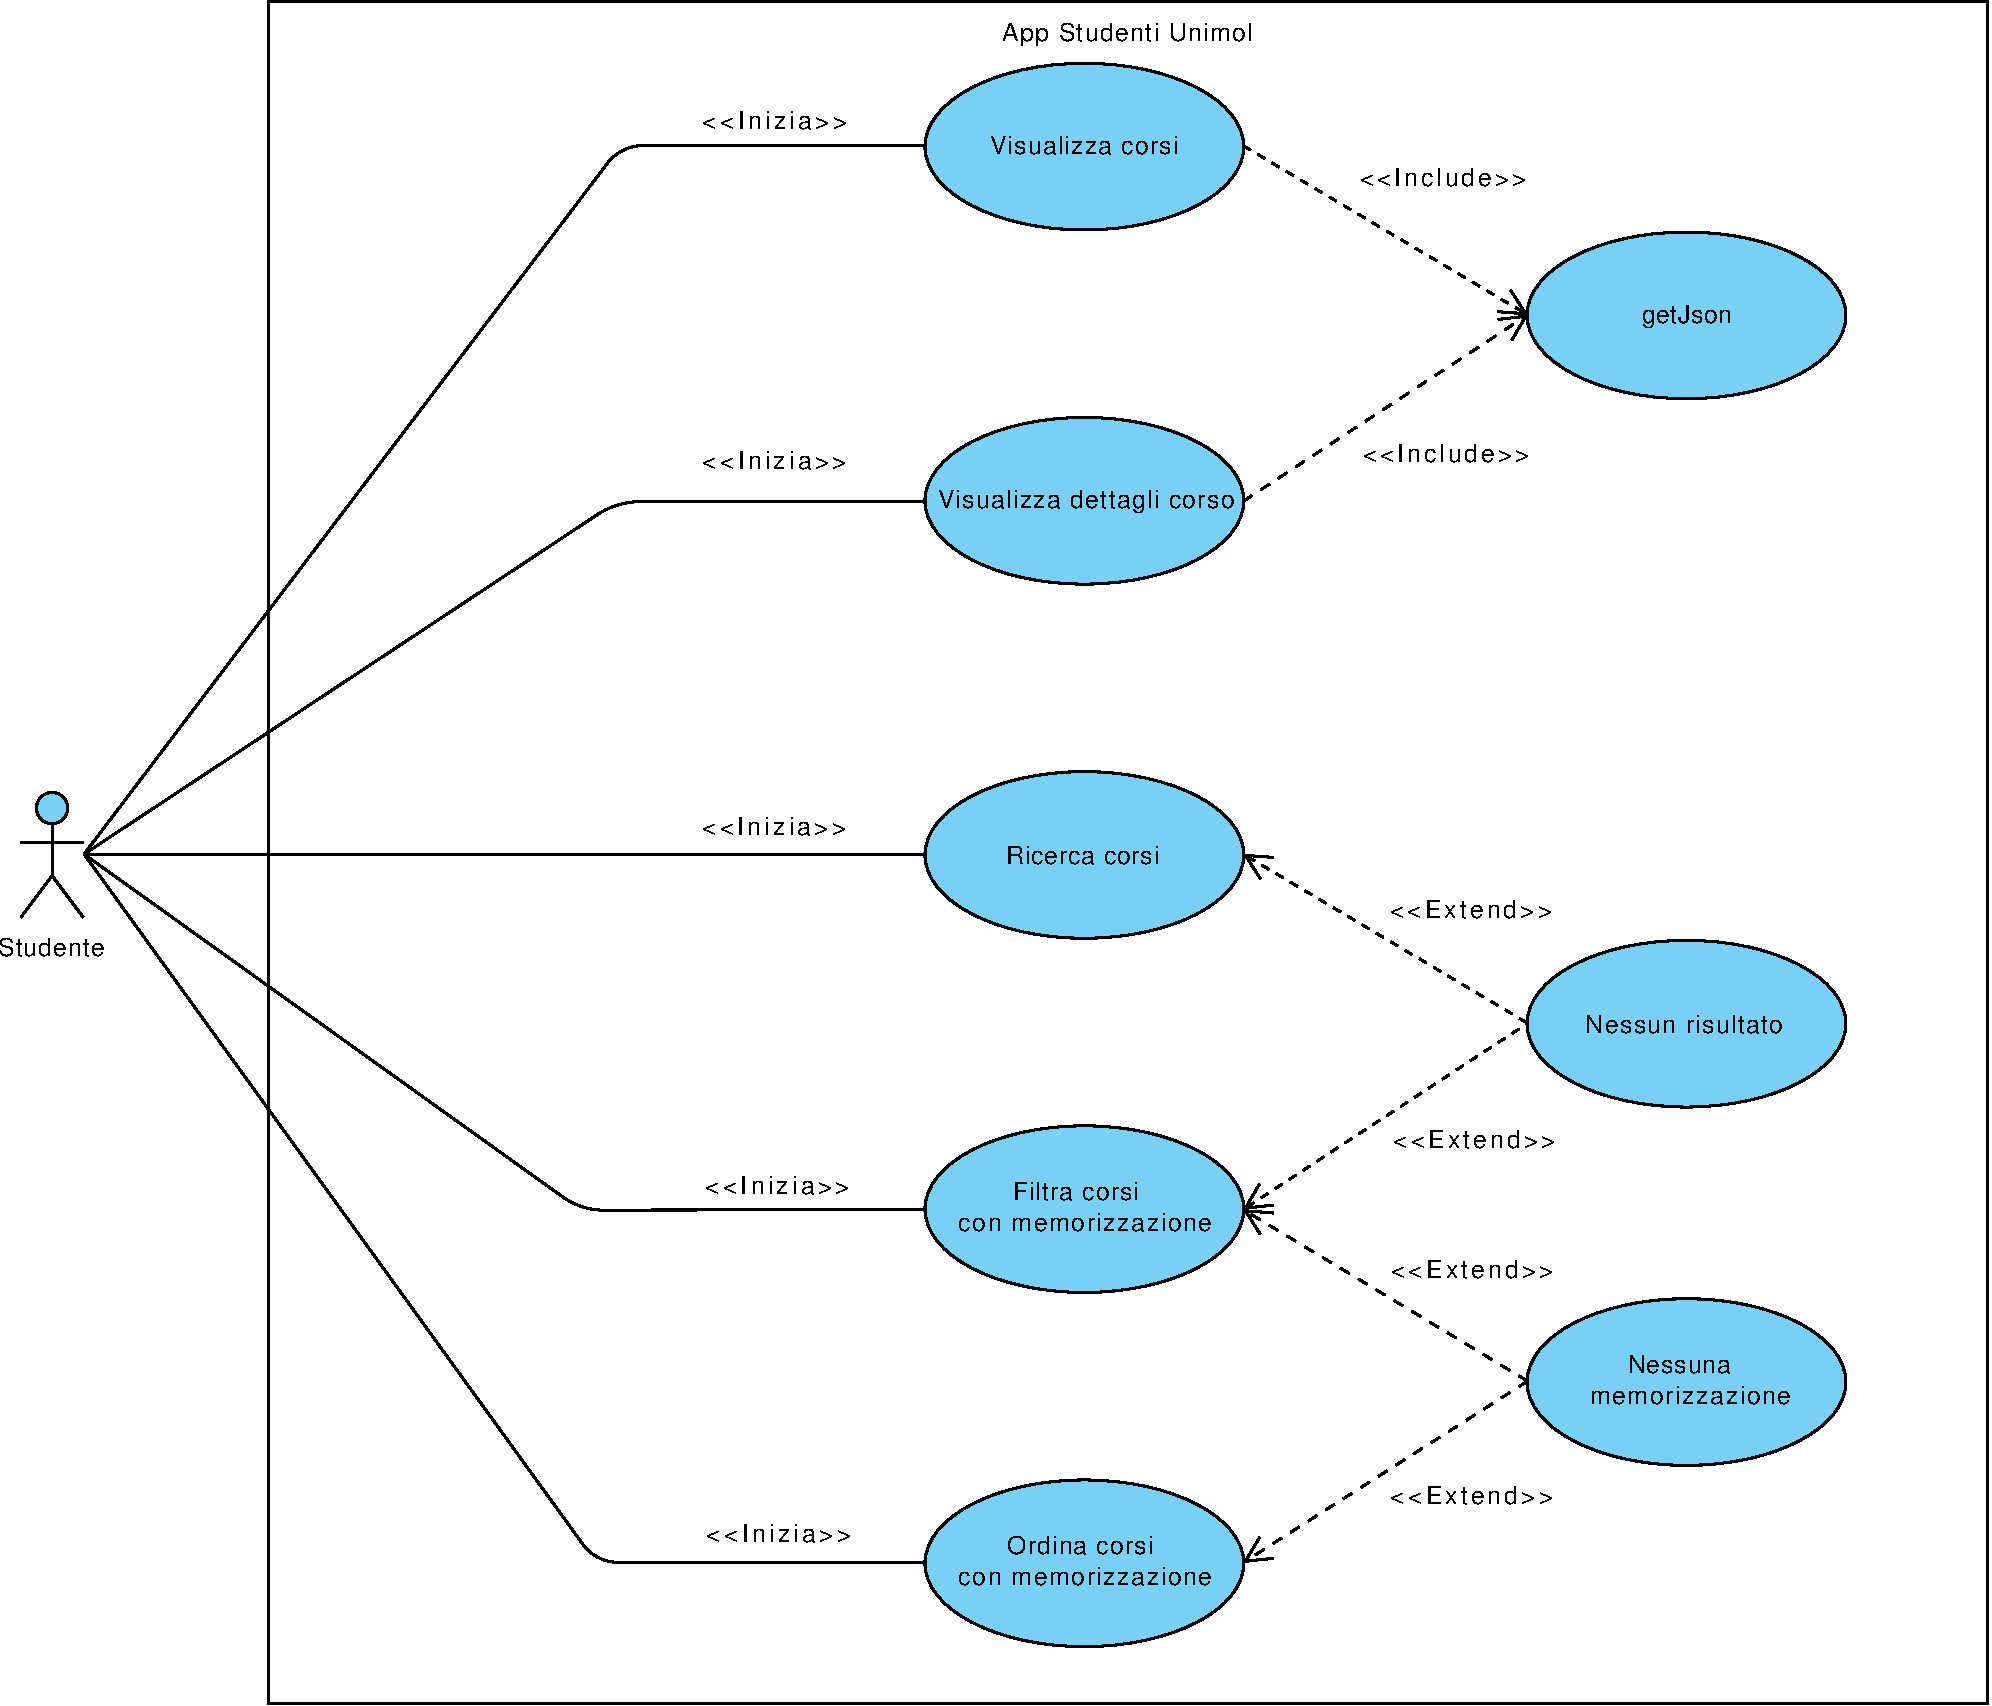
\includegraphics[width=6.5in]{imgs/gruppo1/use_case_diagrams/UCD1-gestione_piano_di_studio.pdf}
\end{center}
\newpage

%% 8.3.2 Appelli %%
\subsection{Gestione appelli}
\begin{center}
	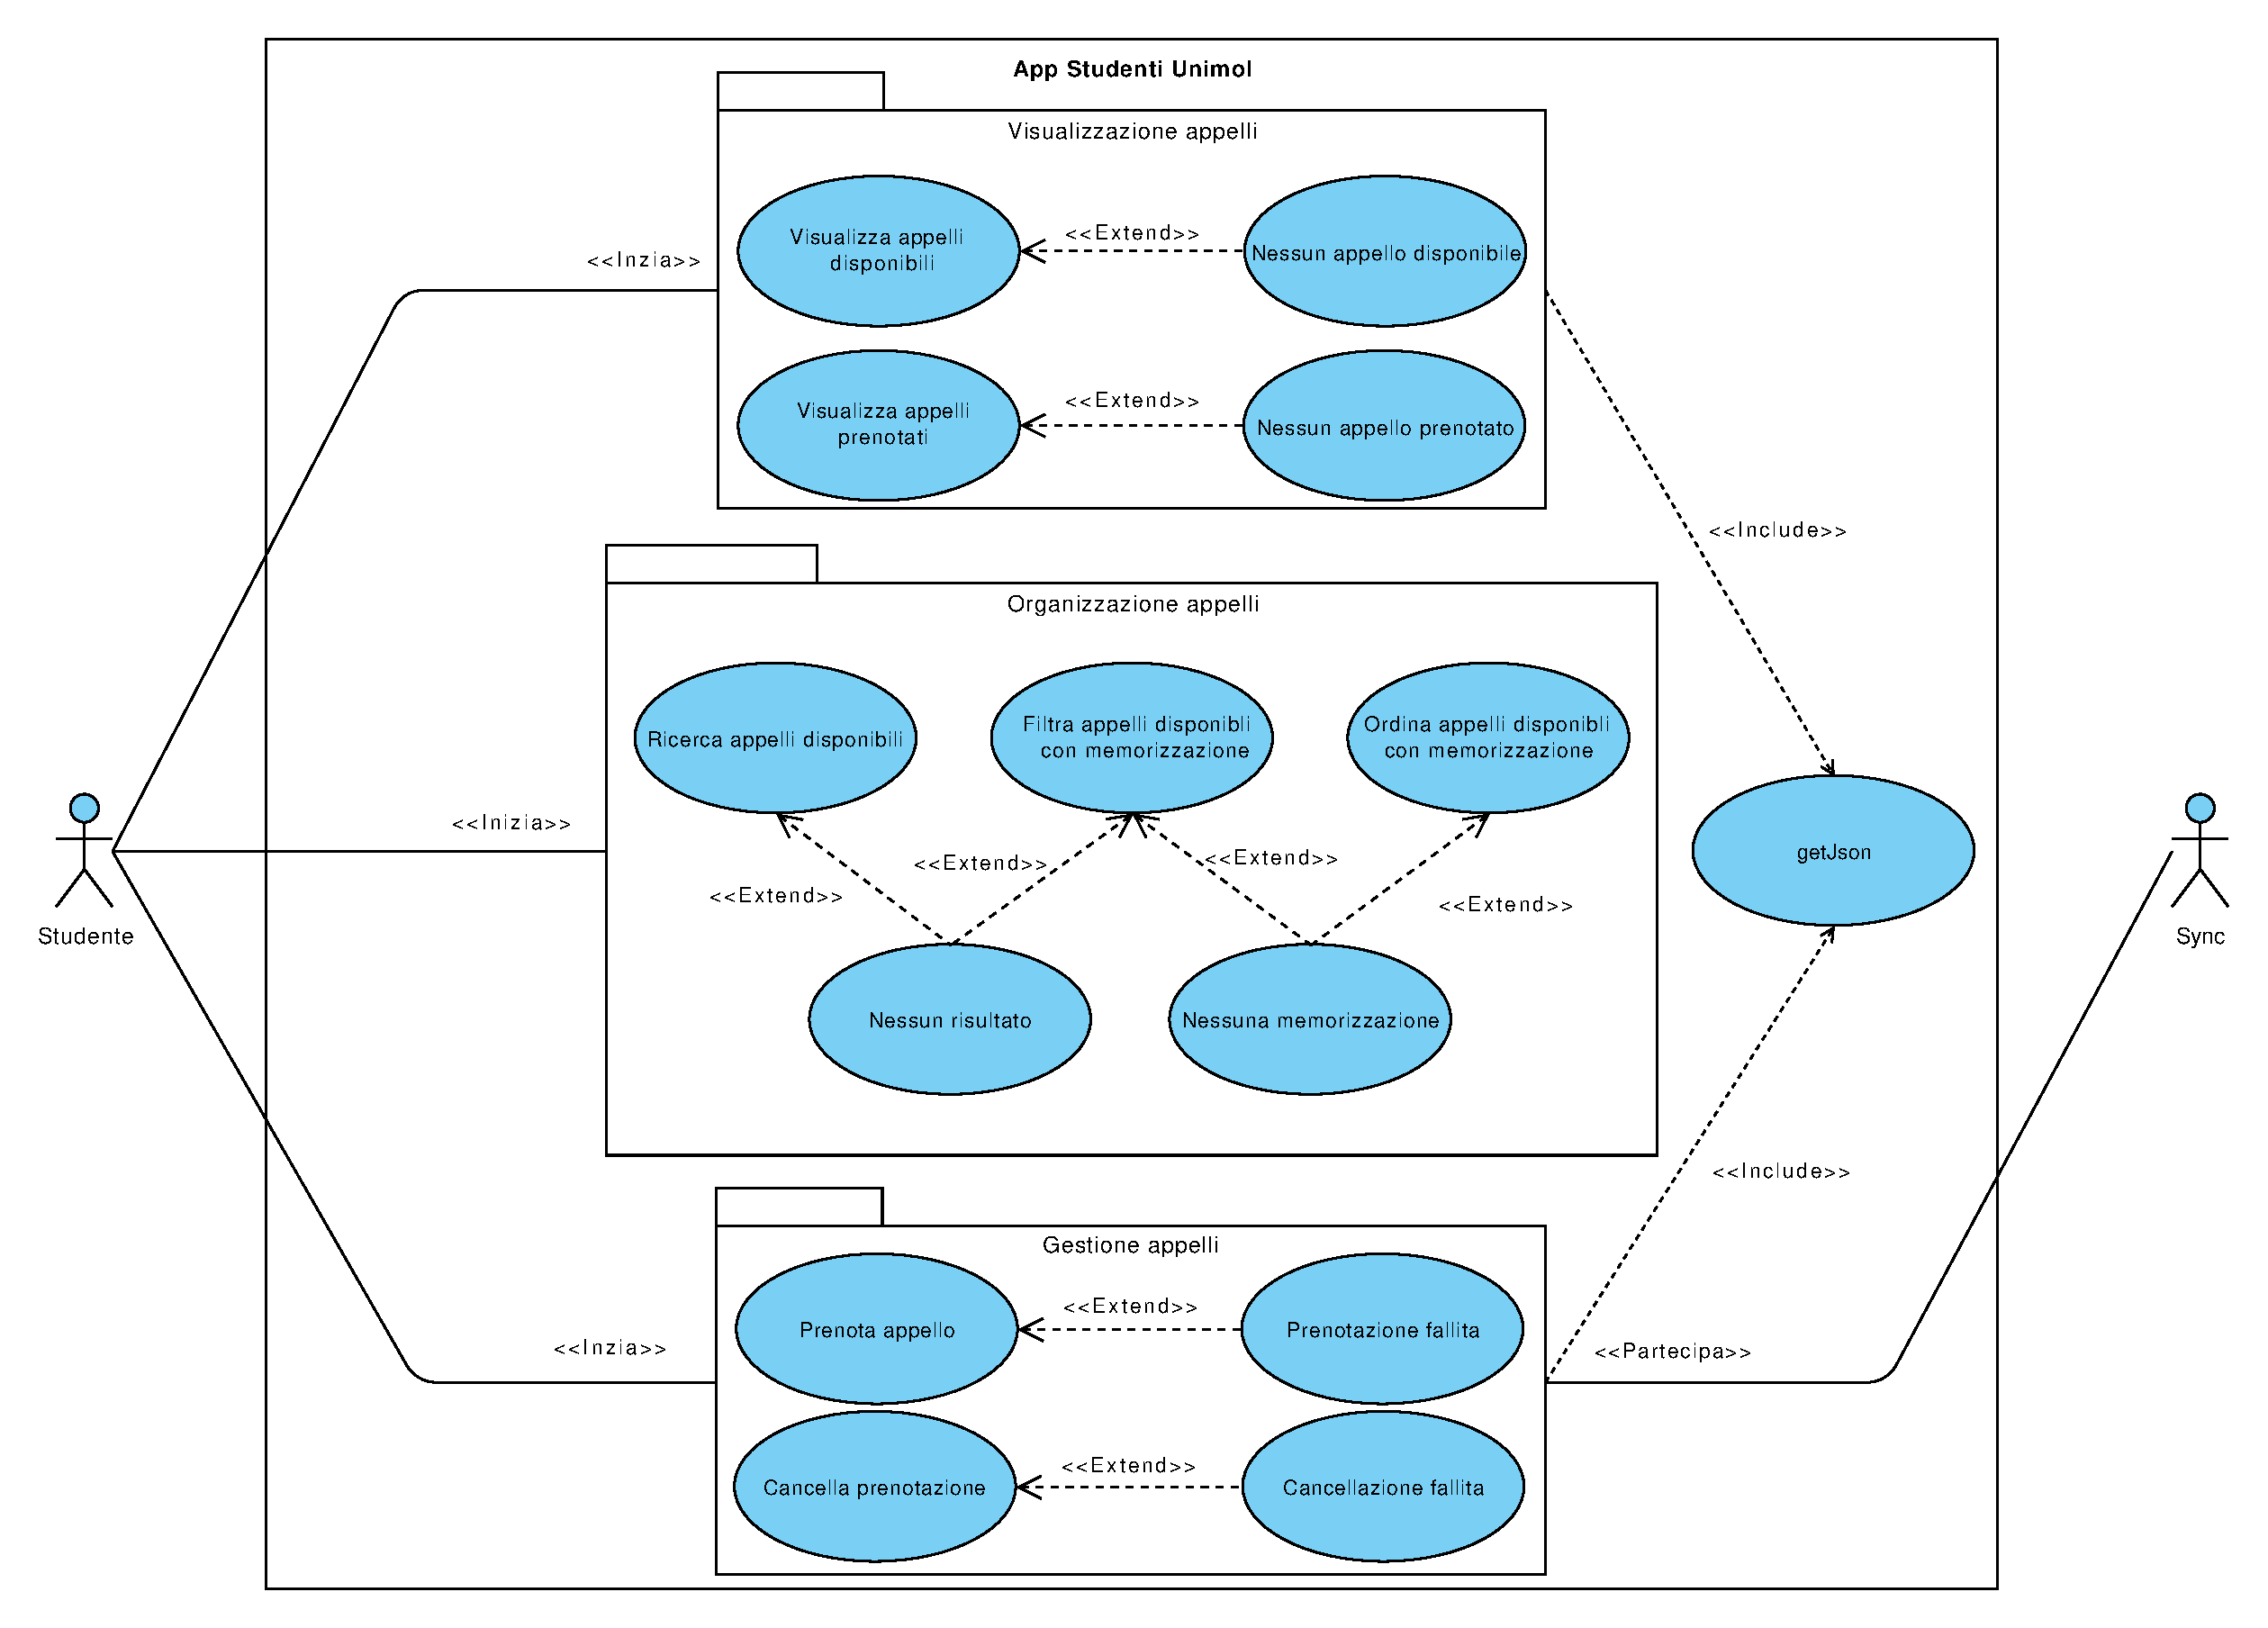
\includegraphics[width=6.5in]{imgs/gruppo1/use_case_diagrams/UCD2-gestione_appelli.pdf}
\end{center}
\newpage

%% 8.3.3 Gestione Materiale Didattico %%
\subsection{Gestione Materiale Didattico}
\begin{center}
	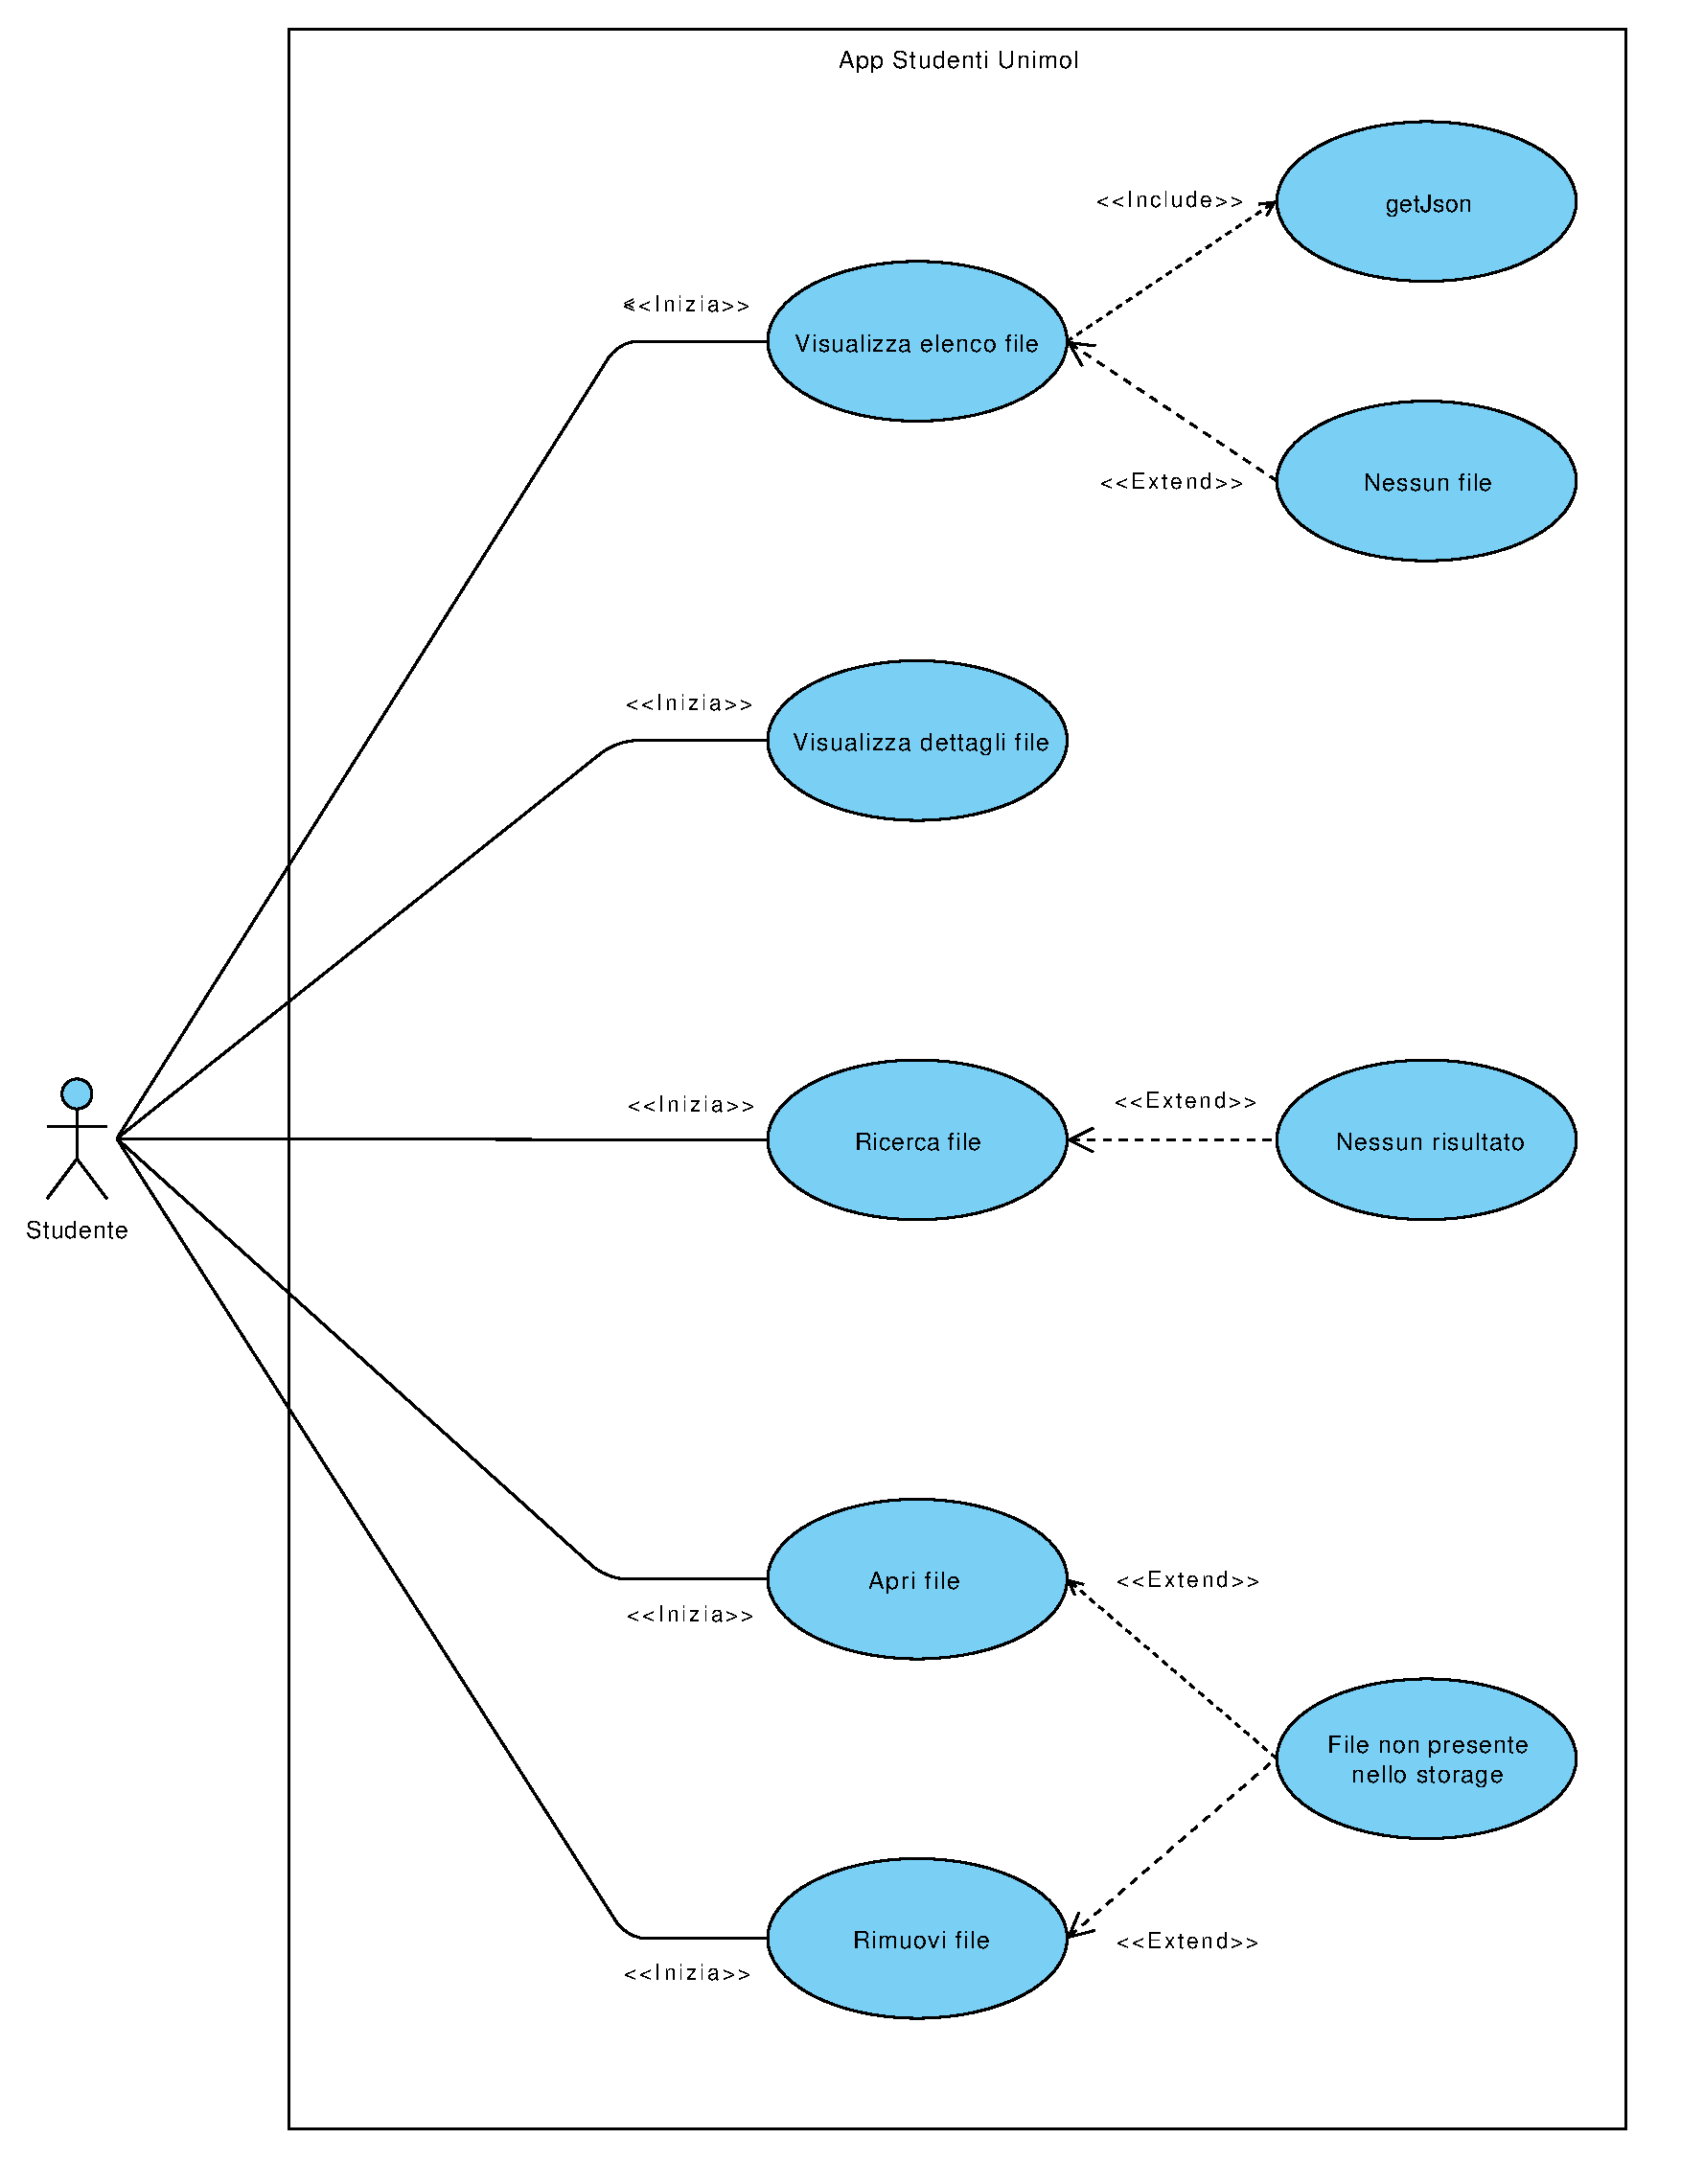
\includegraphics[width=6.5in]{imgs/gruppo1/use_case_diagrams/UCD3-materiale_didattico.pdf}
\end{center}
\newpage




\section{Diagrammi di sequenza}


%%8.5.1 - Visualizza corsi%%
\subsection{Visualizza corsi}
\begin{center}
	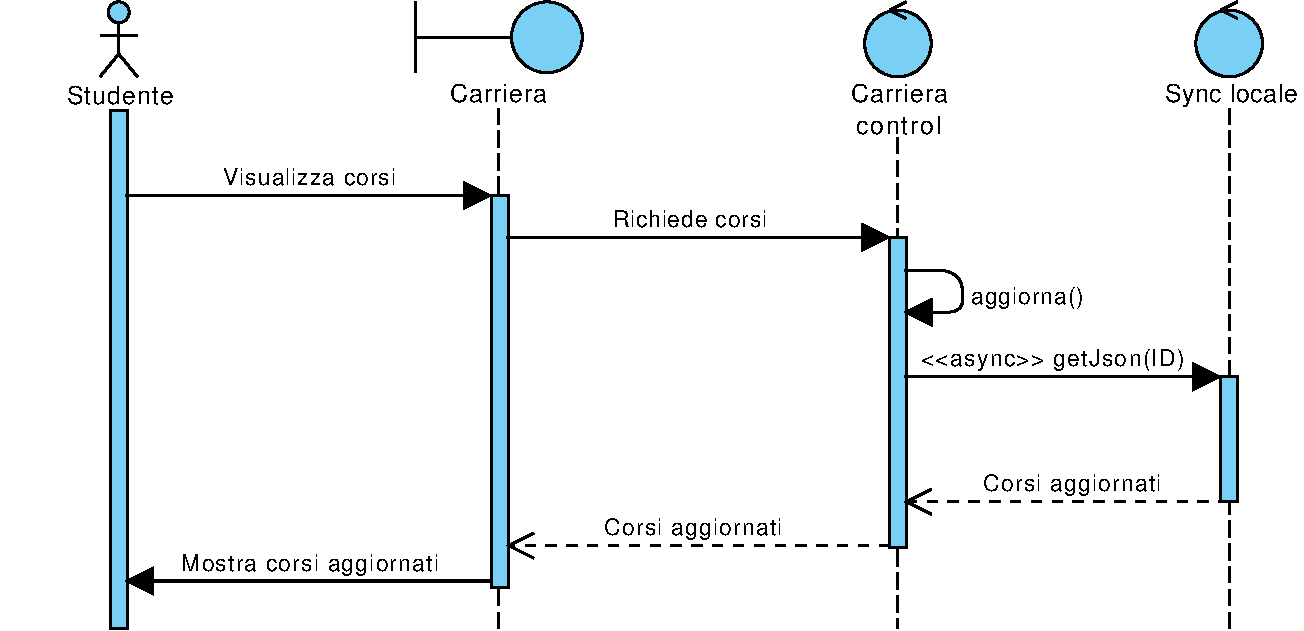
\includegraphics[width=6.5in]{imgs/gruppo1/sequence_diagrams/SD1_visualizza_corsi.pdf}
\end{center}
%%8.5.2 - Ricerca corsi%%
\subsection{Ricerca corsi}
\begin{center}
	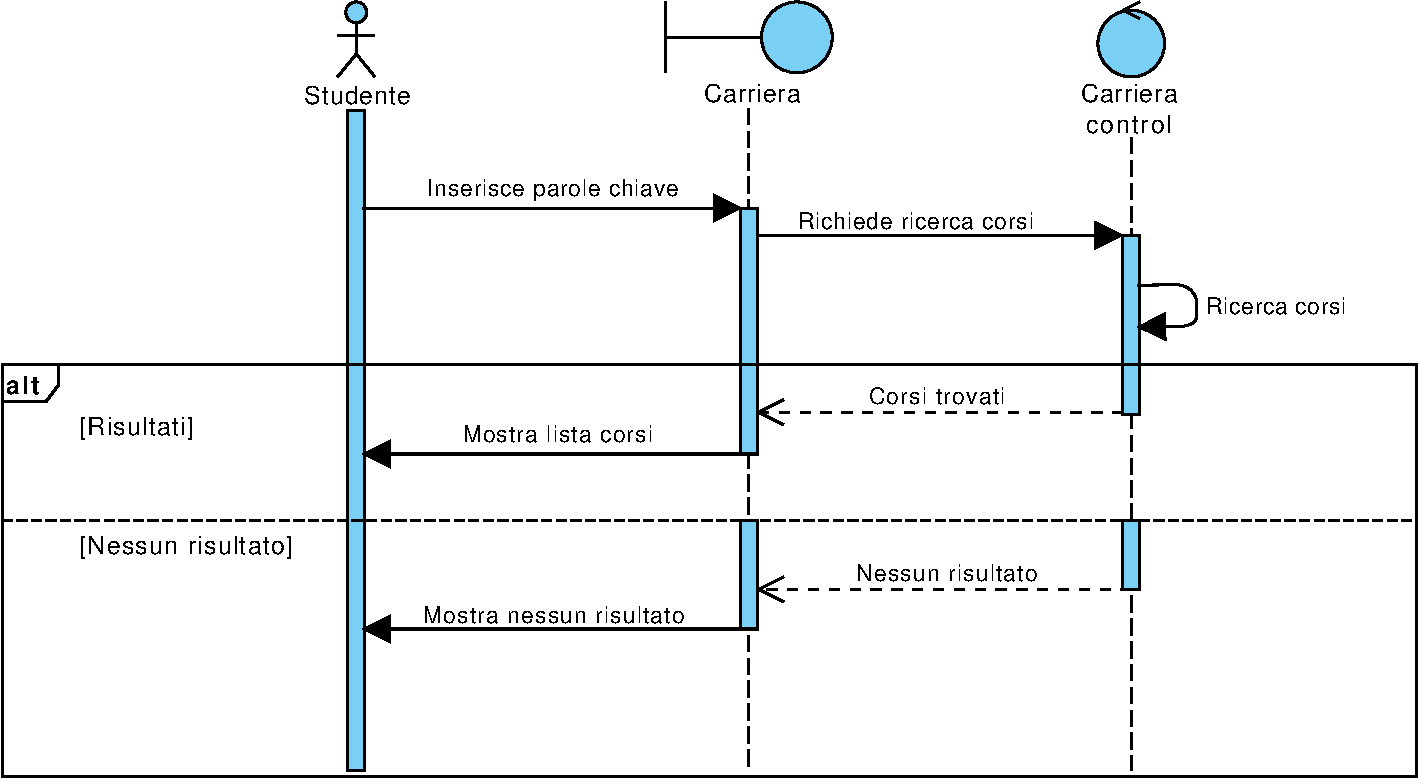
\includegraphics[width=6.5in]{imgs/gruppo1/sequence_diagrams/SD2_ricerca_corsi.pdf}
\end{center}
\newpage


%%8.5.3 - Filtra corsi con memorizzazione%%
\subsection{Filtra corsi con memorizzazione}
\begin{center}
	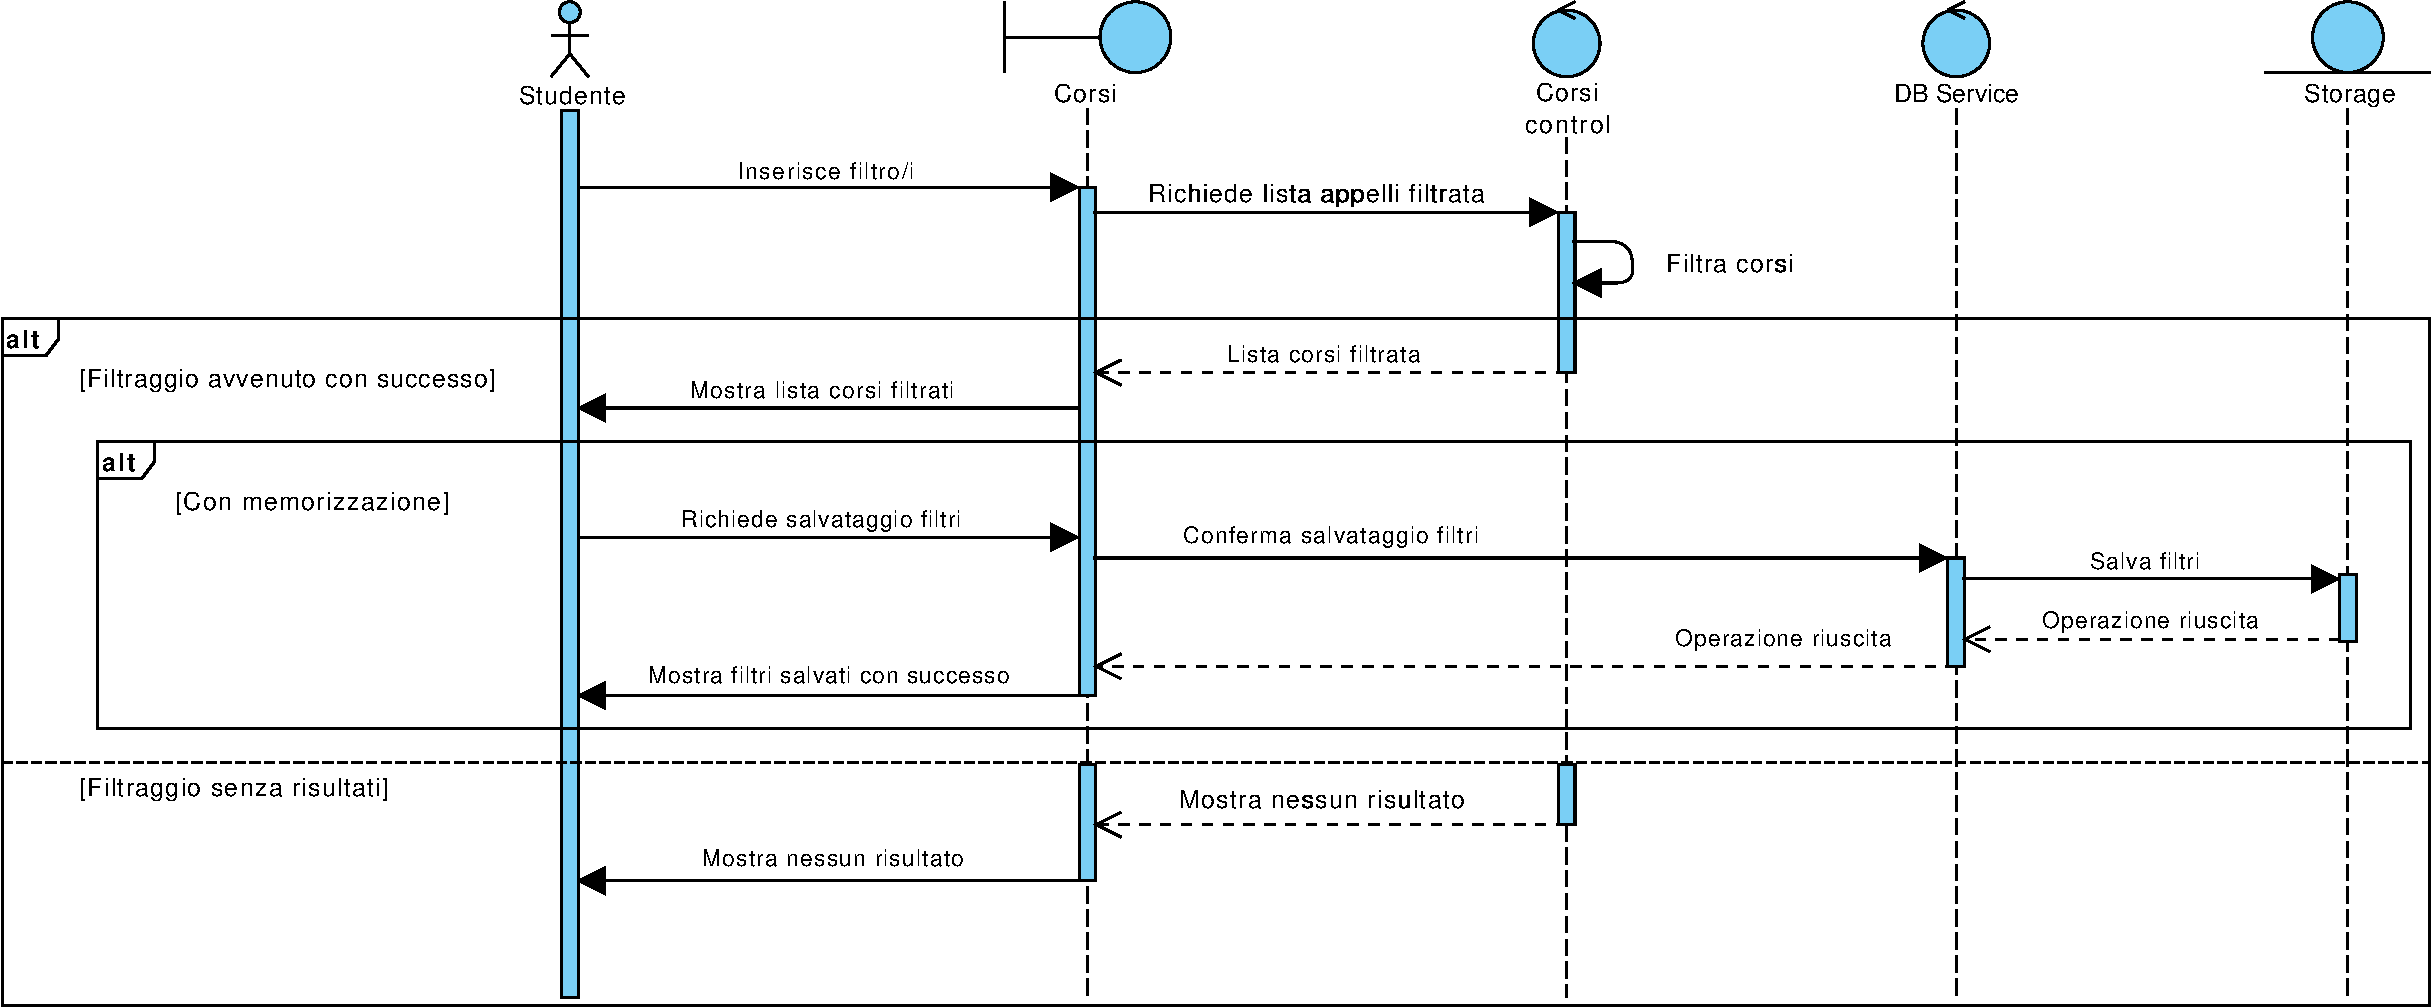
\includegraphics[width=6.5in]{imgs/gruppo1/sequence_diagrams/SD3_filtra_corsi_con_memorizzazione.pdf}
\end{center}
%%8.5.4 - Ordina corsi con memorizzazione%%
\subsection{Ordina corsi con memorizzazione}
\begin{center}
	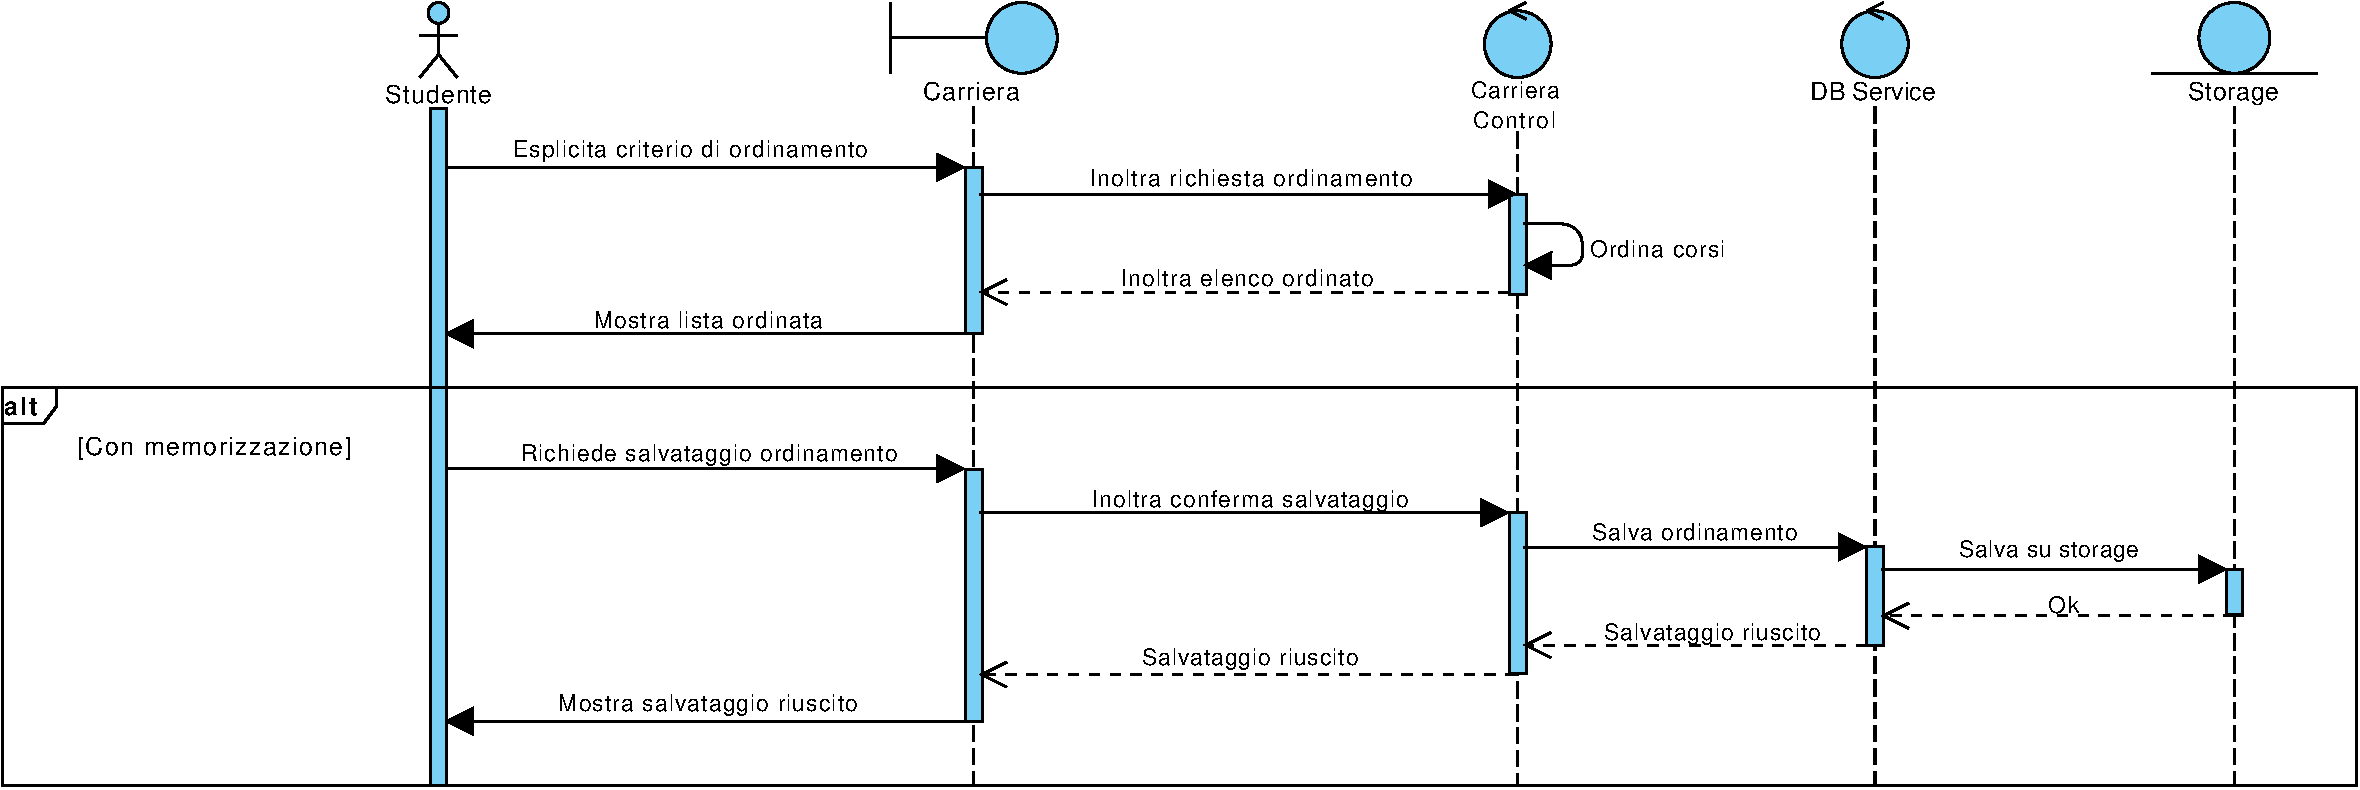
\includegraphics[width=6.5in]{imgs/gruppo1/sequence_diagrams/SD4_ordina_corsi_con_memorizzazione.pdf}
\end{center}
\newpage


%%8.5.5 - Visualizza dettagli corso%%
\subsection{Visualizza dettagli corso}
\begin{center}
	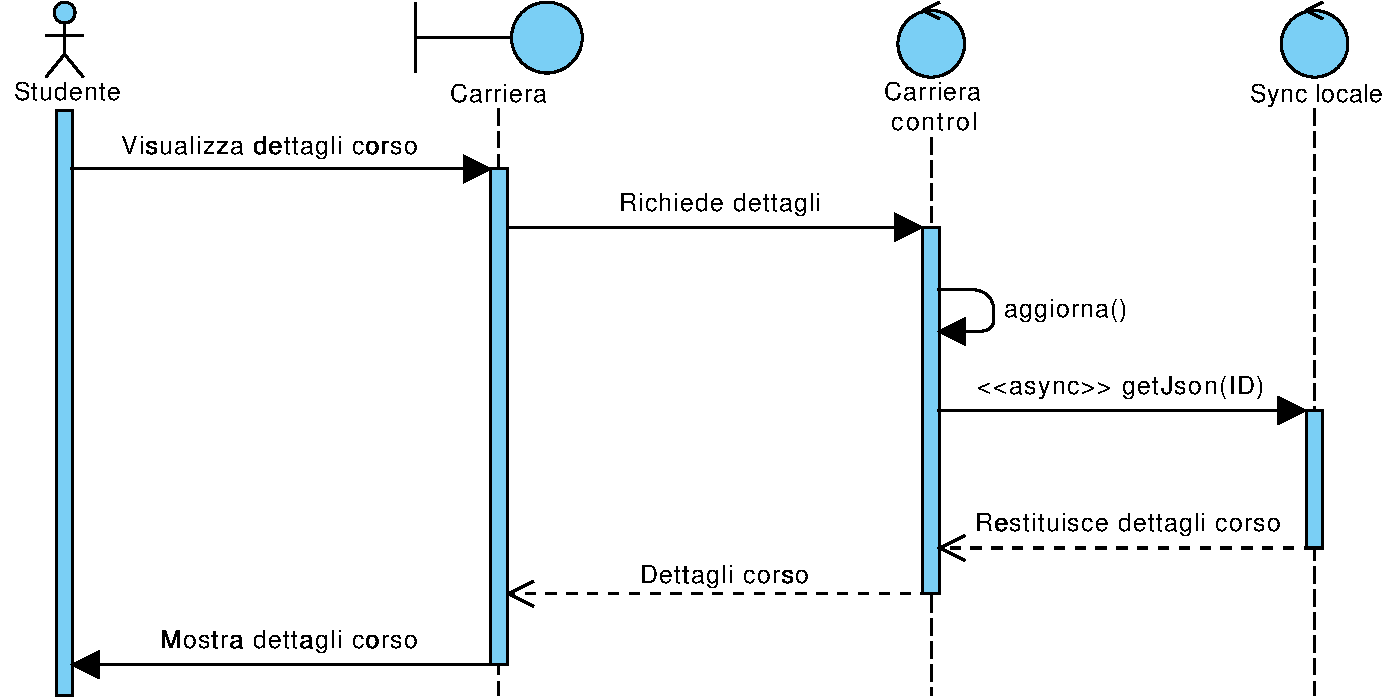
\includegraphics[width=6.5in]{imgs/gruppo1/sequence_diagrams/SD5_visualizza_dettagli_corso.pdf}
\end{center}
%%8.5.6 - Visualizza appelli disponibili %%
\subsection{Visualizza appelli disponibili}
\begin{center}
	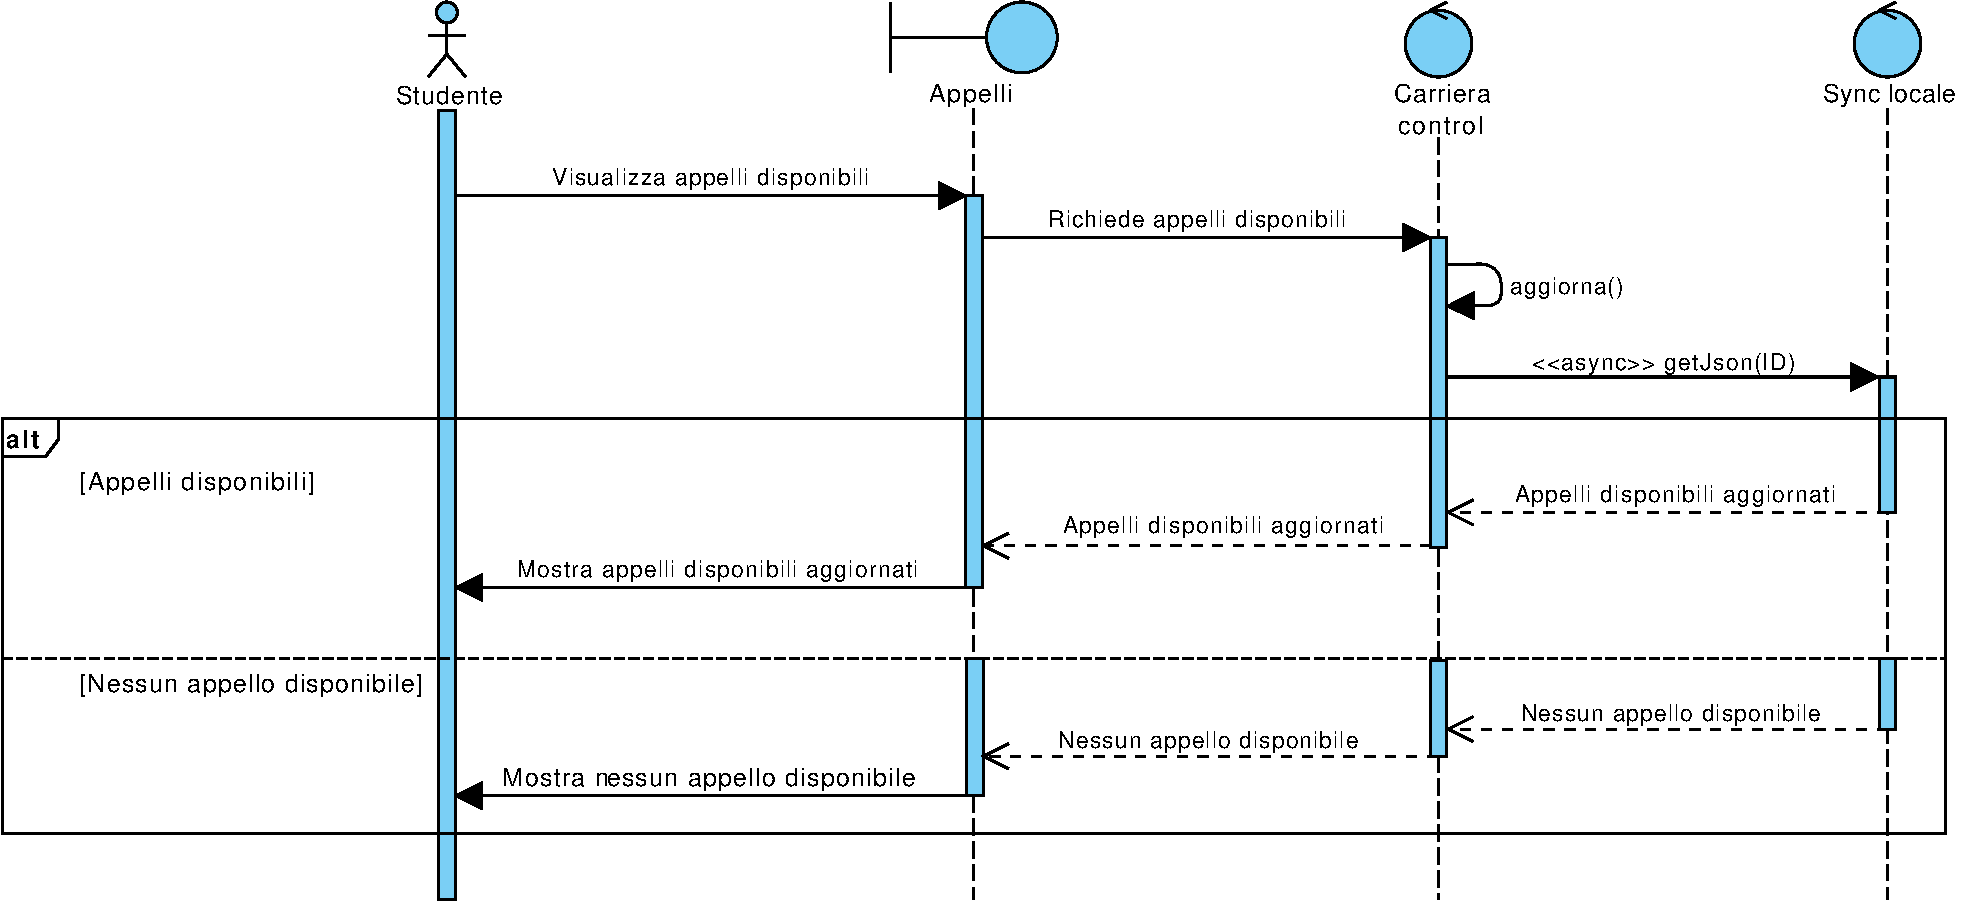
\includegraphics[width=6.5in]{imgs/gruppo1/sequence_diagrams/SD6_visualizza_appelli_disponibili.pdf}
\end{center}
\newpage


%%8.5.7 - Visualizza appelli prenotati  %%
\subsection{Visualizza appelli prenotati}
\begin{center}
	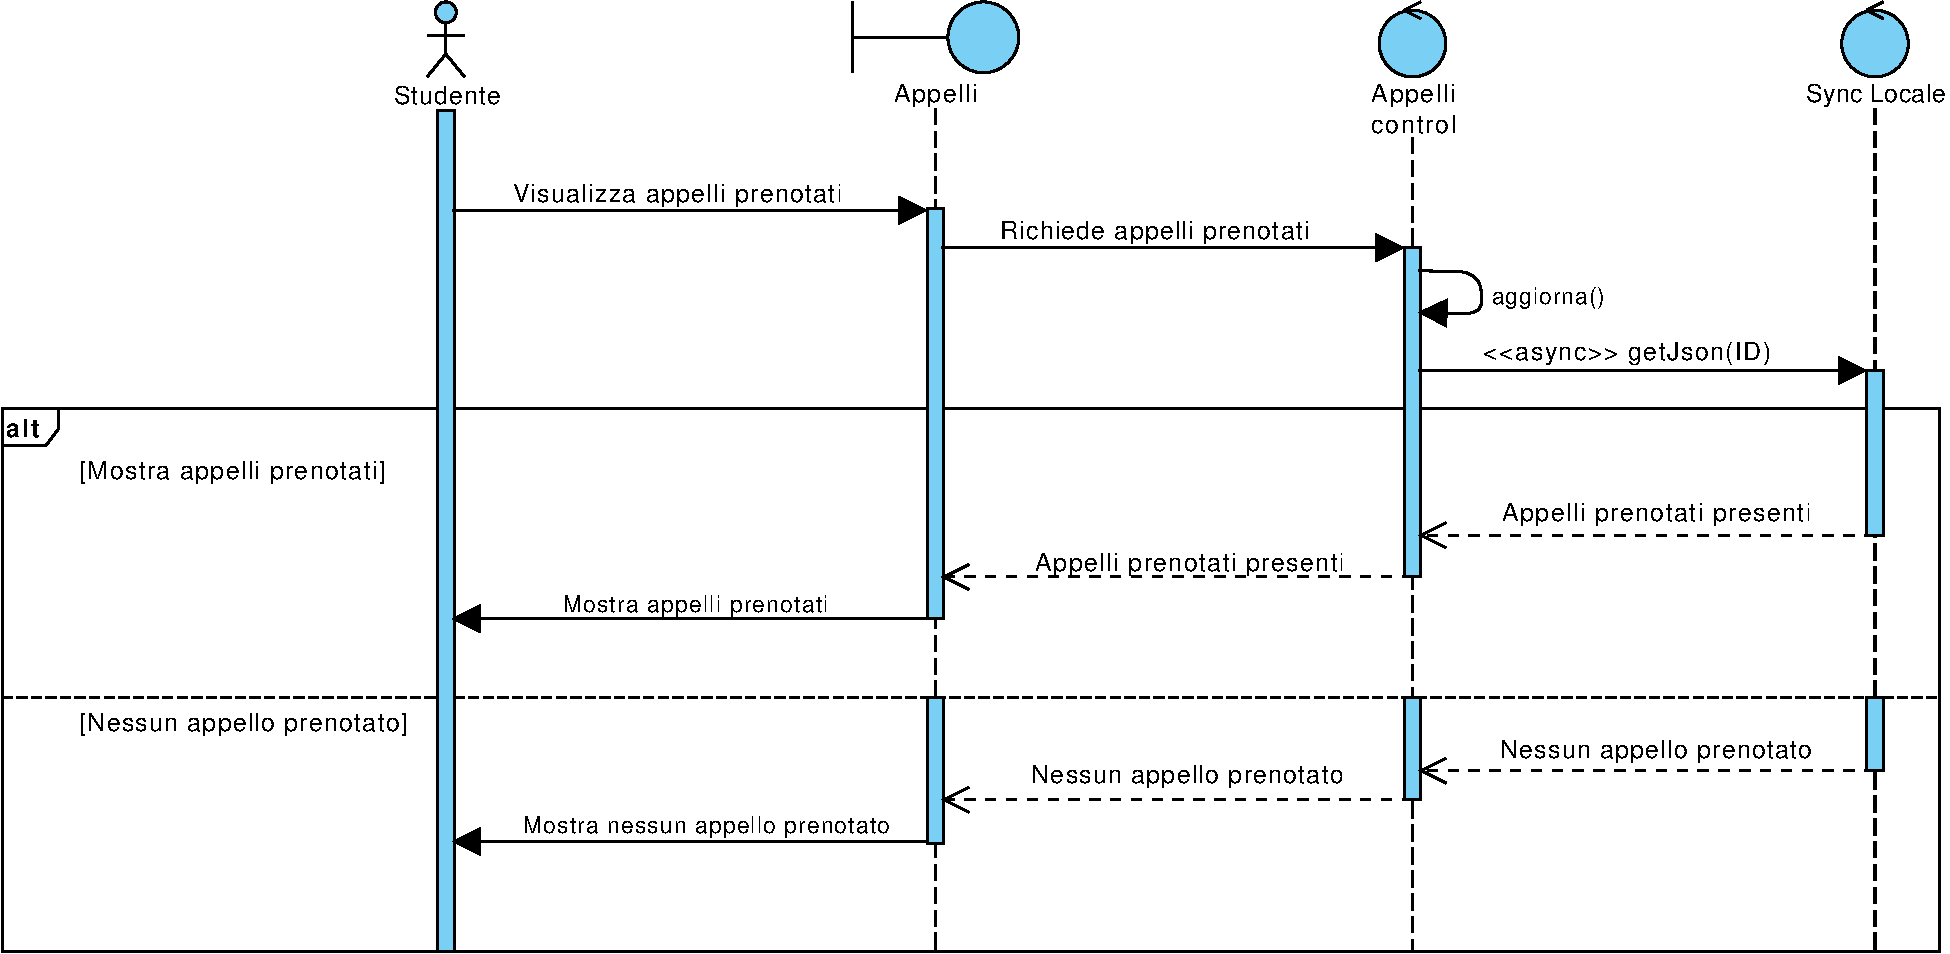
\includegraphics[width=6.5in]{imgs/gruppo1/sequence_diagrams/SD7_visualizza_appelli_prenotati.pdf}
\end{center}
%% 8.5.8 - Ricerca appelli disponibili  %%
\subsection{Ricerca appelli disponibili}
\begin{center}
	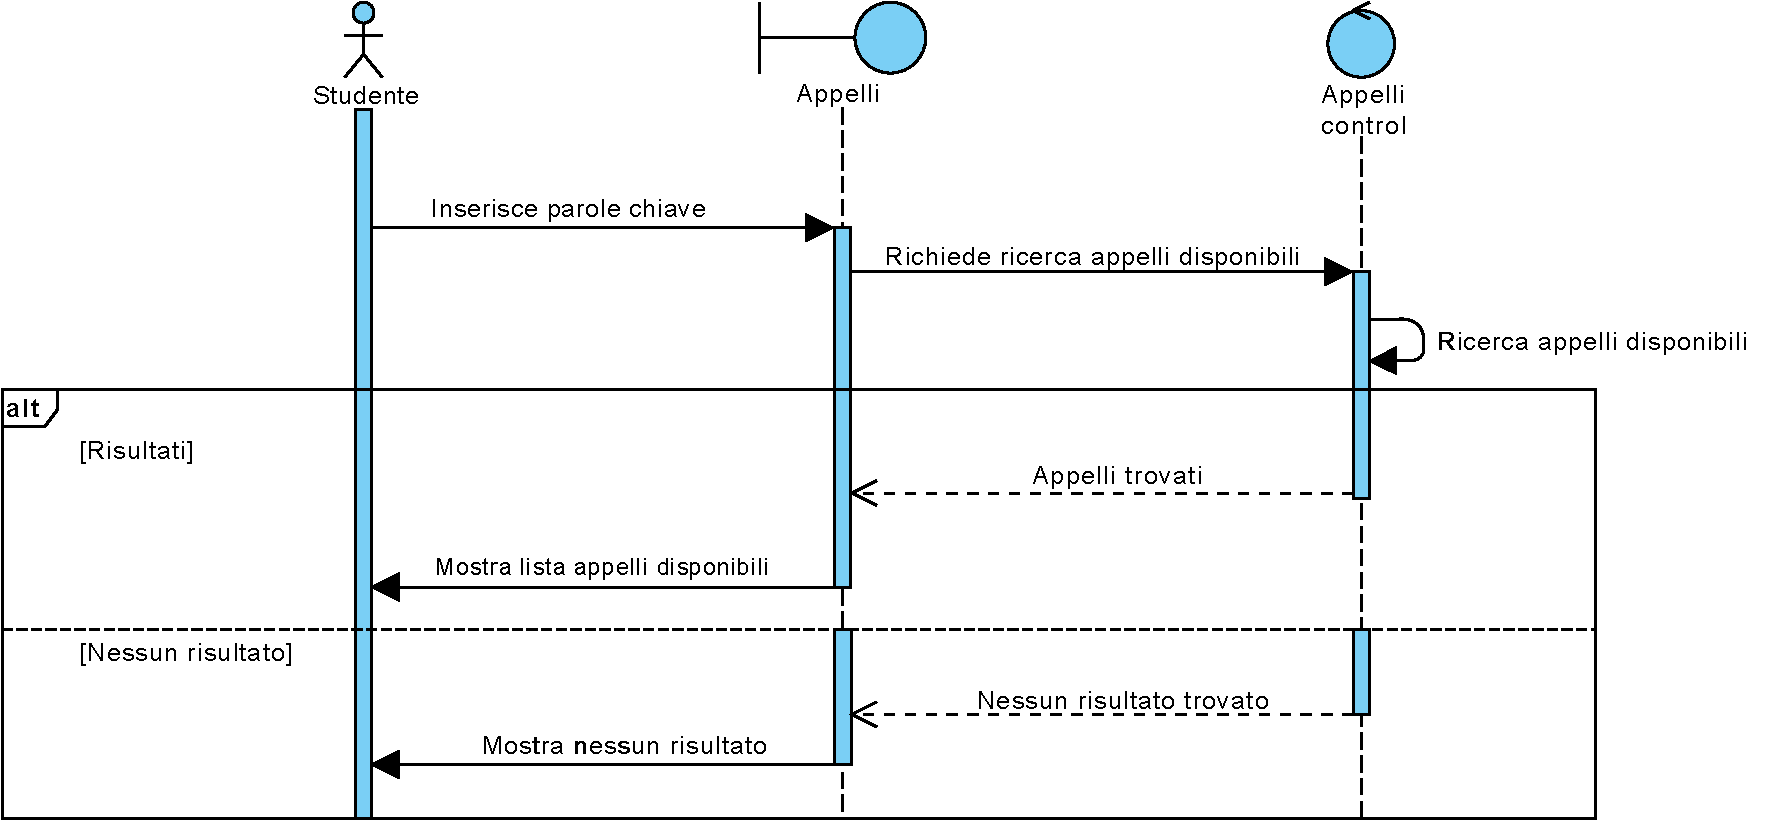
\includegraphics[width=6.5in]{imgs/gruppo1/sequence_diagrams/SD8_ricerca_appelli_disponibili.pdf}
\end{center}
\newpage


%% 8.5.9 - Filtra appelli disponibili con memorizzazione  %%
\subsection{Filtra appelli disponibili con memorizzazione}
\begin{center}
	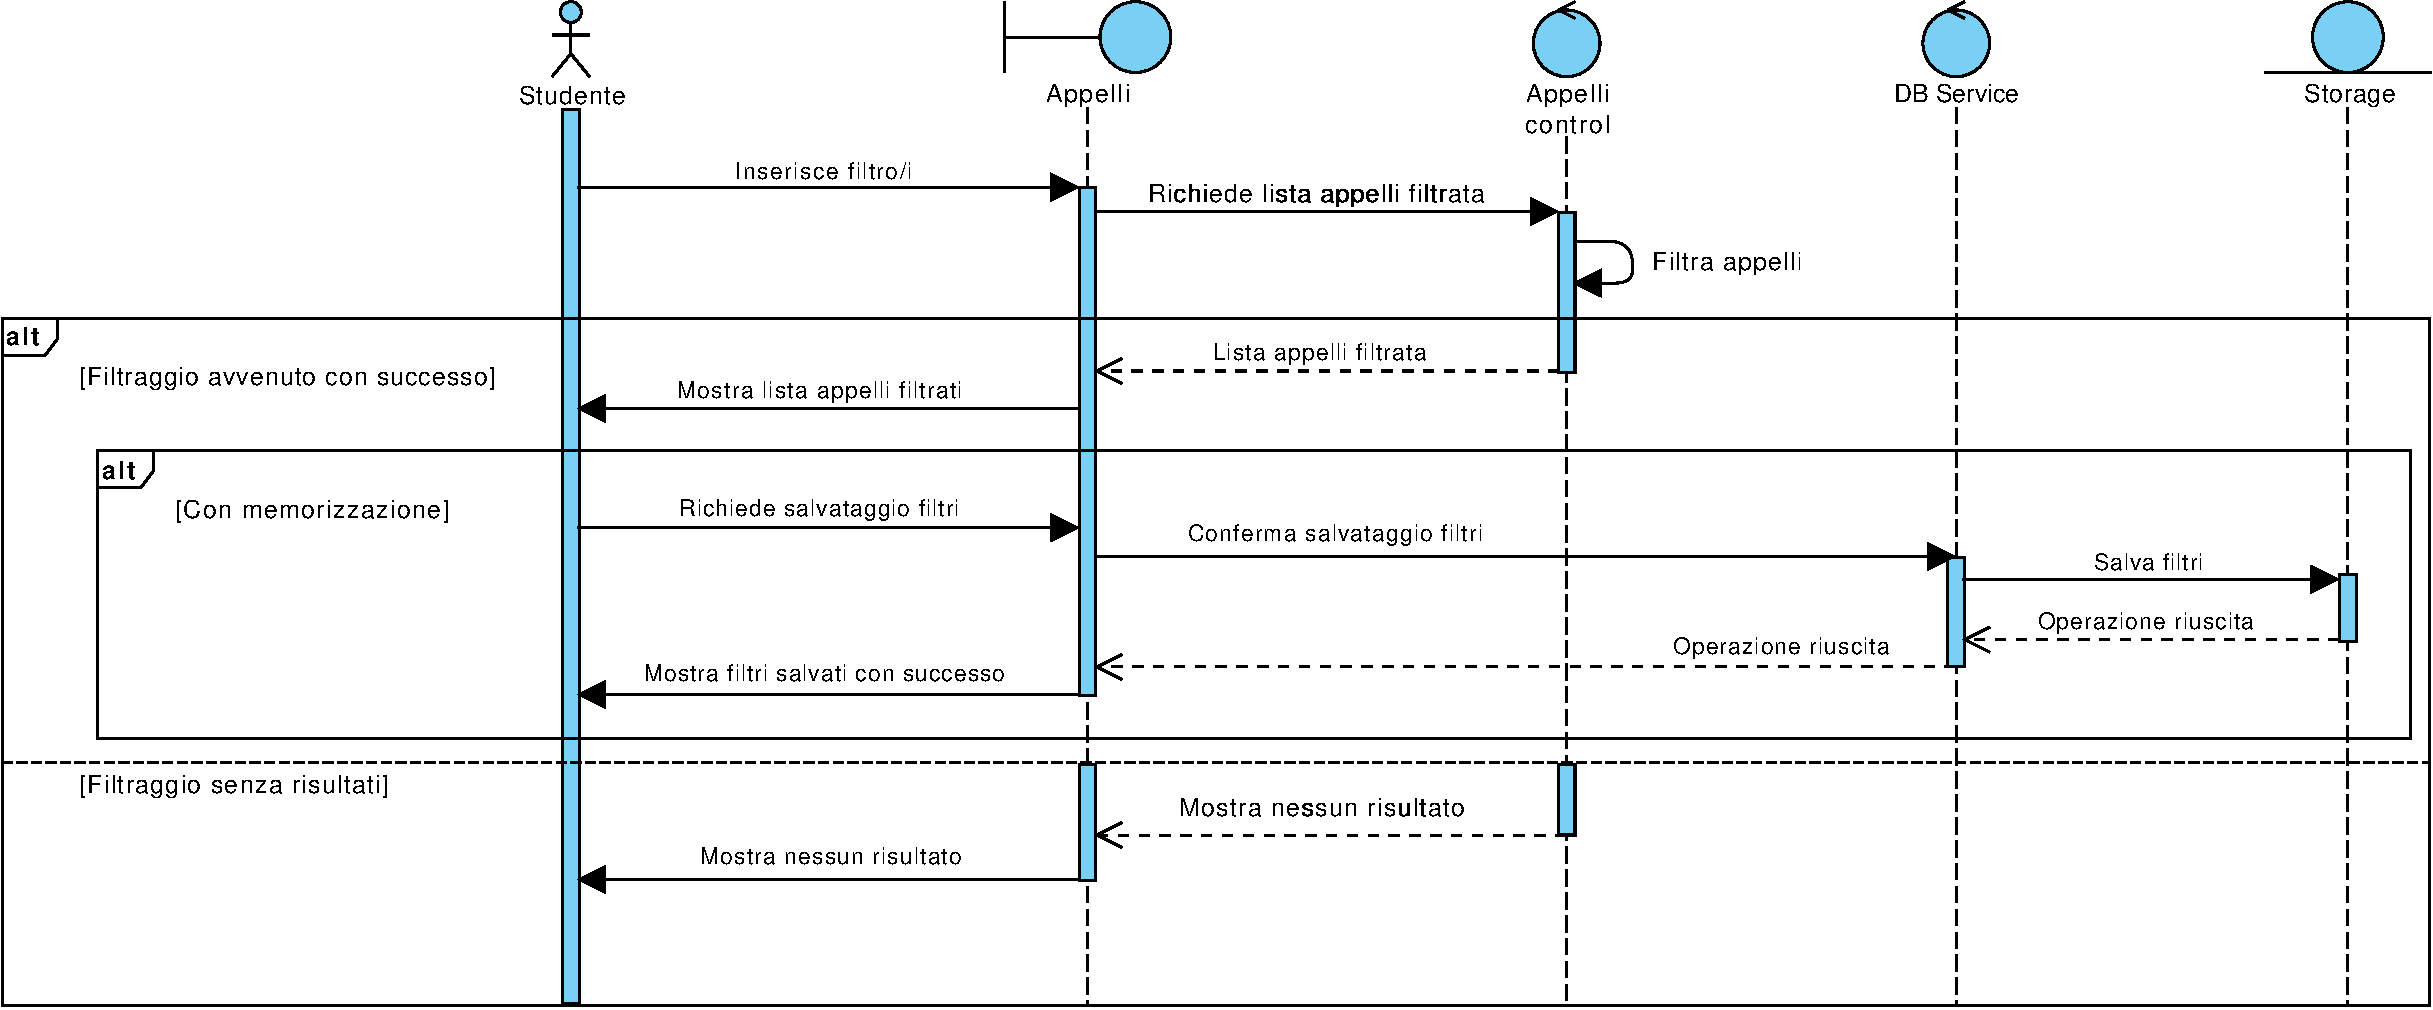
\includegraphics[width=6.5in]{imgs/gruppo1/sequence_diagrams/SD9_filtra_appelli_disponibili_con_memorizzazione.pdf}
\end{center}
%% 8.5.10 - Ordina appelli disponibili con memorizzazione  %%
\subsection{Ordina appelli disponibili con memorizzazione}
\begin{center}
	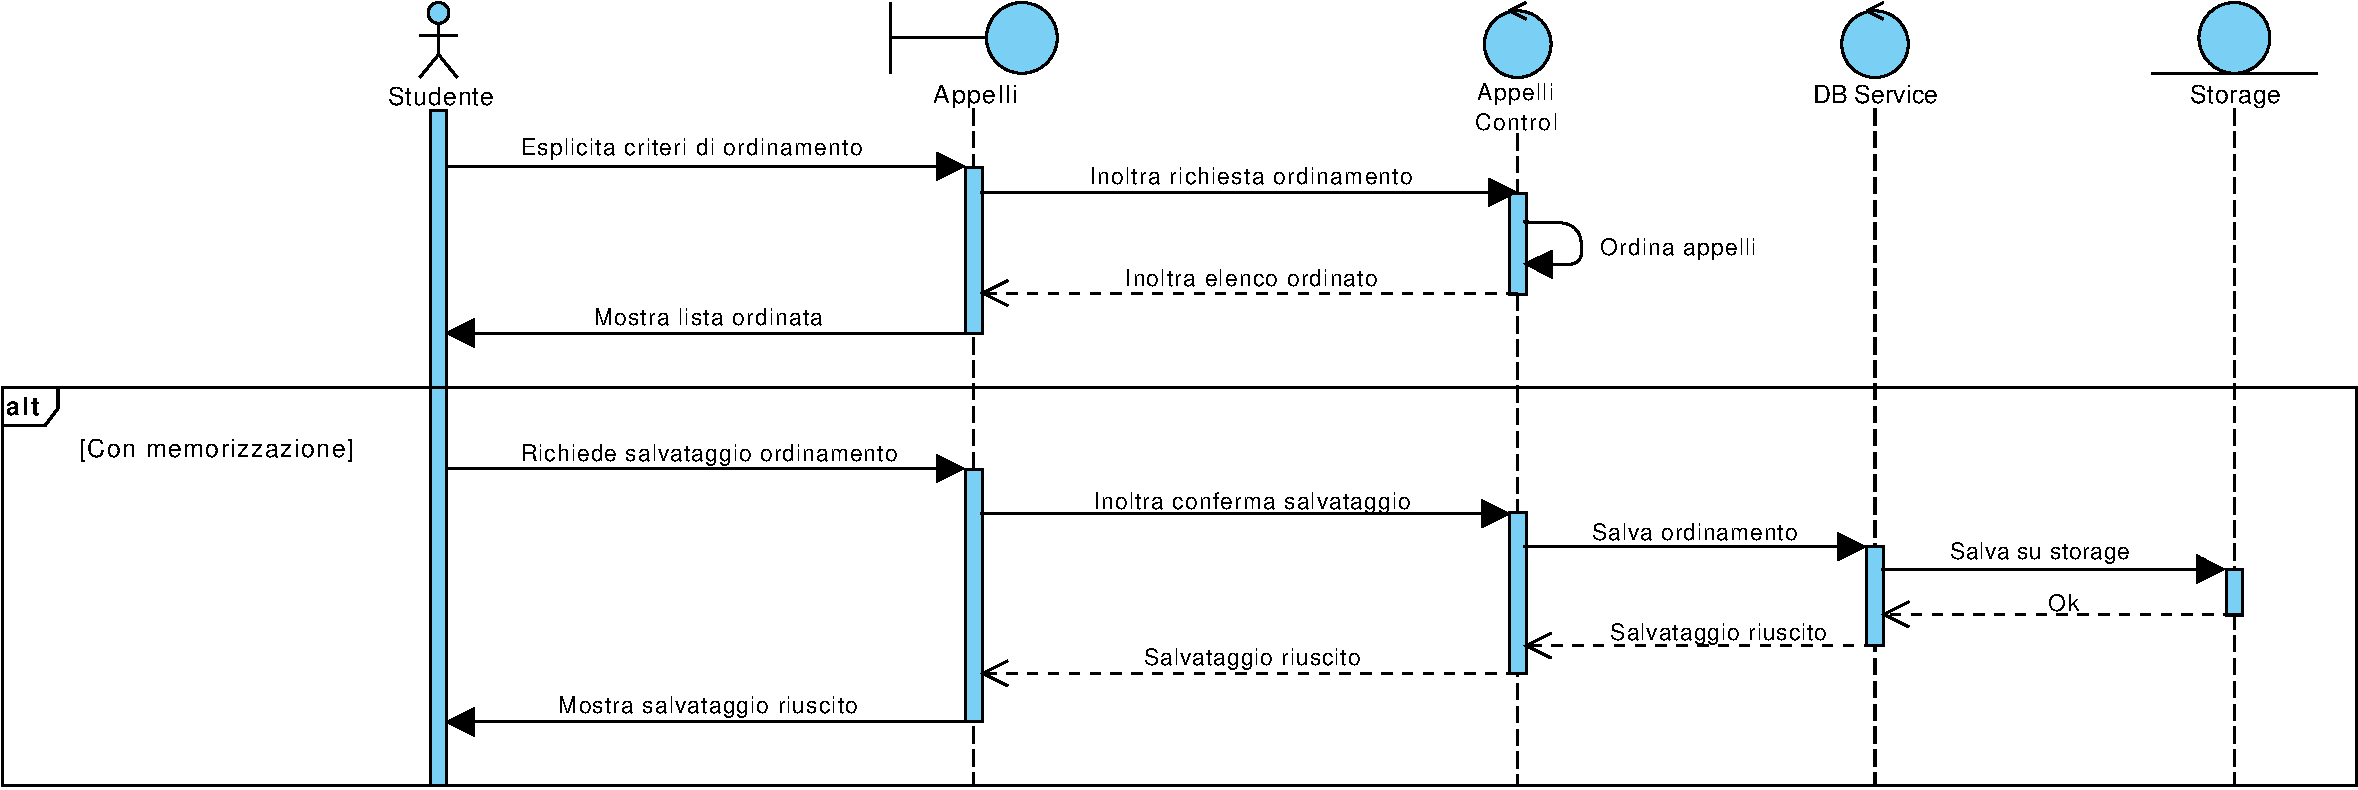
\includegraphics[width=6.5in]{imgs/gruppo1/sequence_diagrams/SD10_ordina_appelli_disponibili_con_memorizzazione.pdf}
\end{center}
\newpage

%%  8.5.11 - Prenota appello  %%
\subsection{Prenota appello}
\begin{center}
	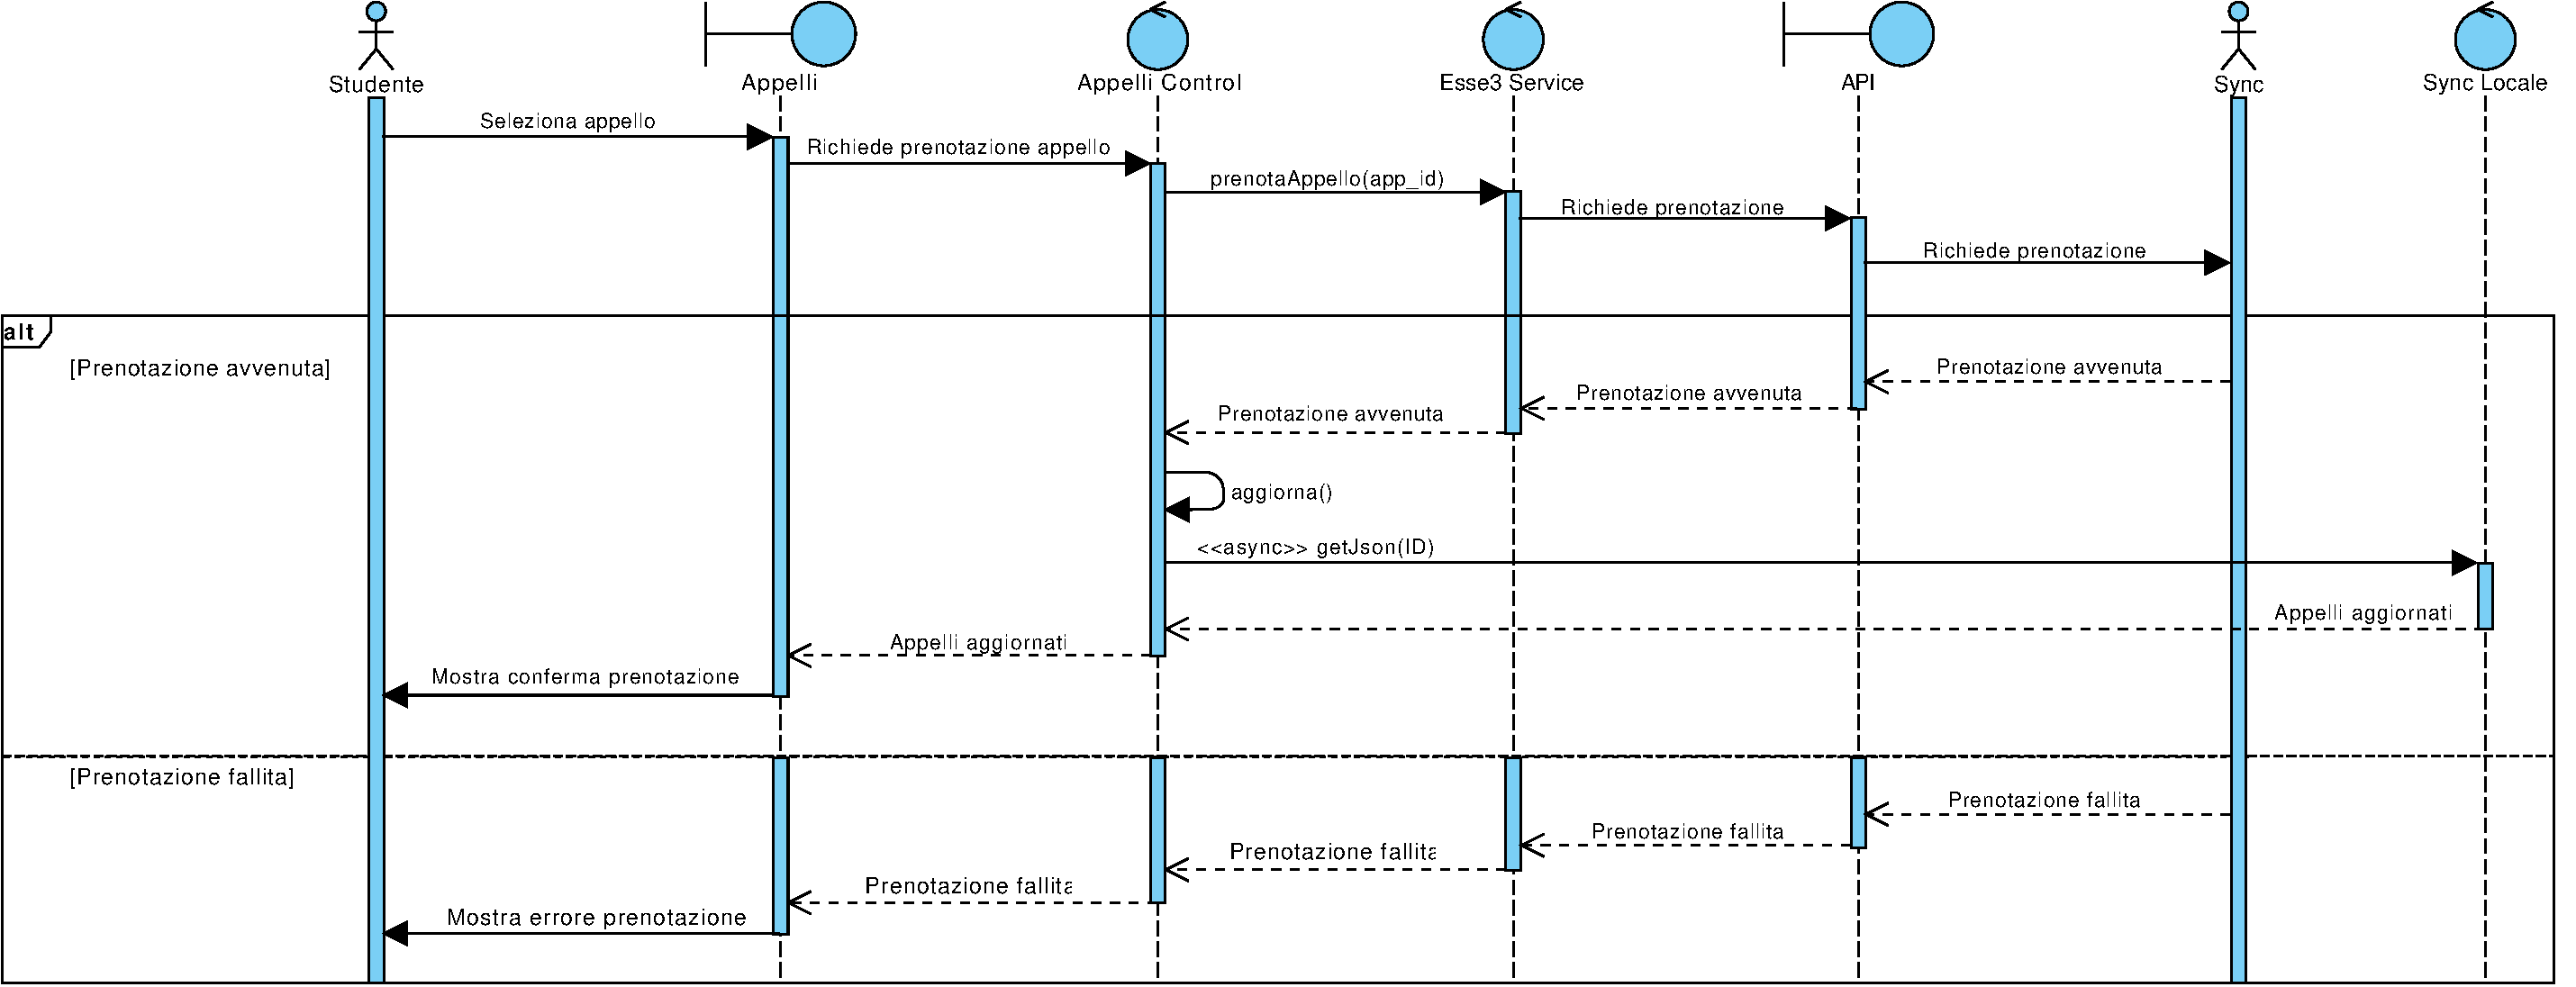
\includegraphics[width=6.5in]{imgs/gruppo1/sequence_diagrams/SD11_prenota_appello.pdf}
\end{center}
%% 8.5.12 - Cancella prenotazione   %%
\subsection{Cancella prenotazione}
\begin{center}
	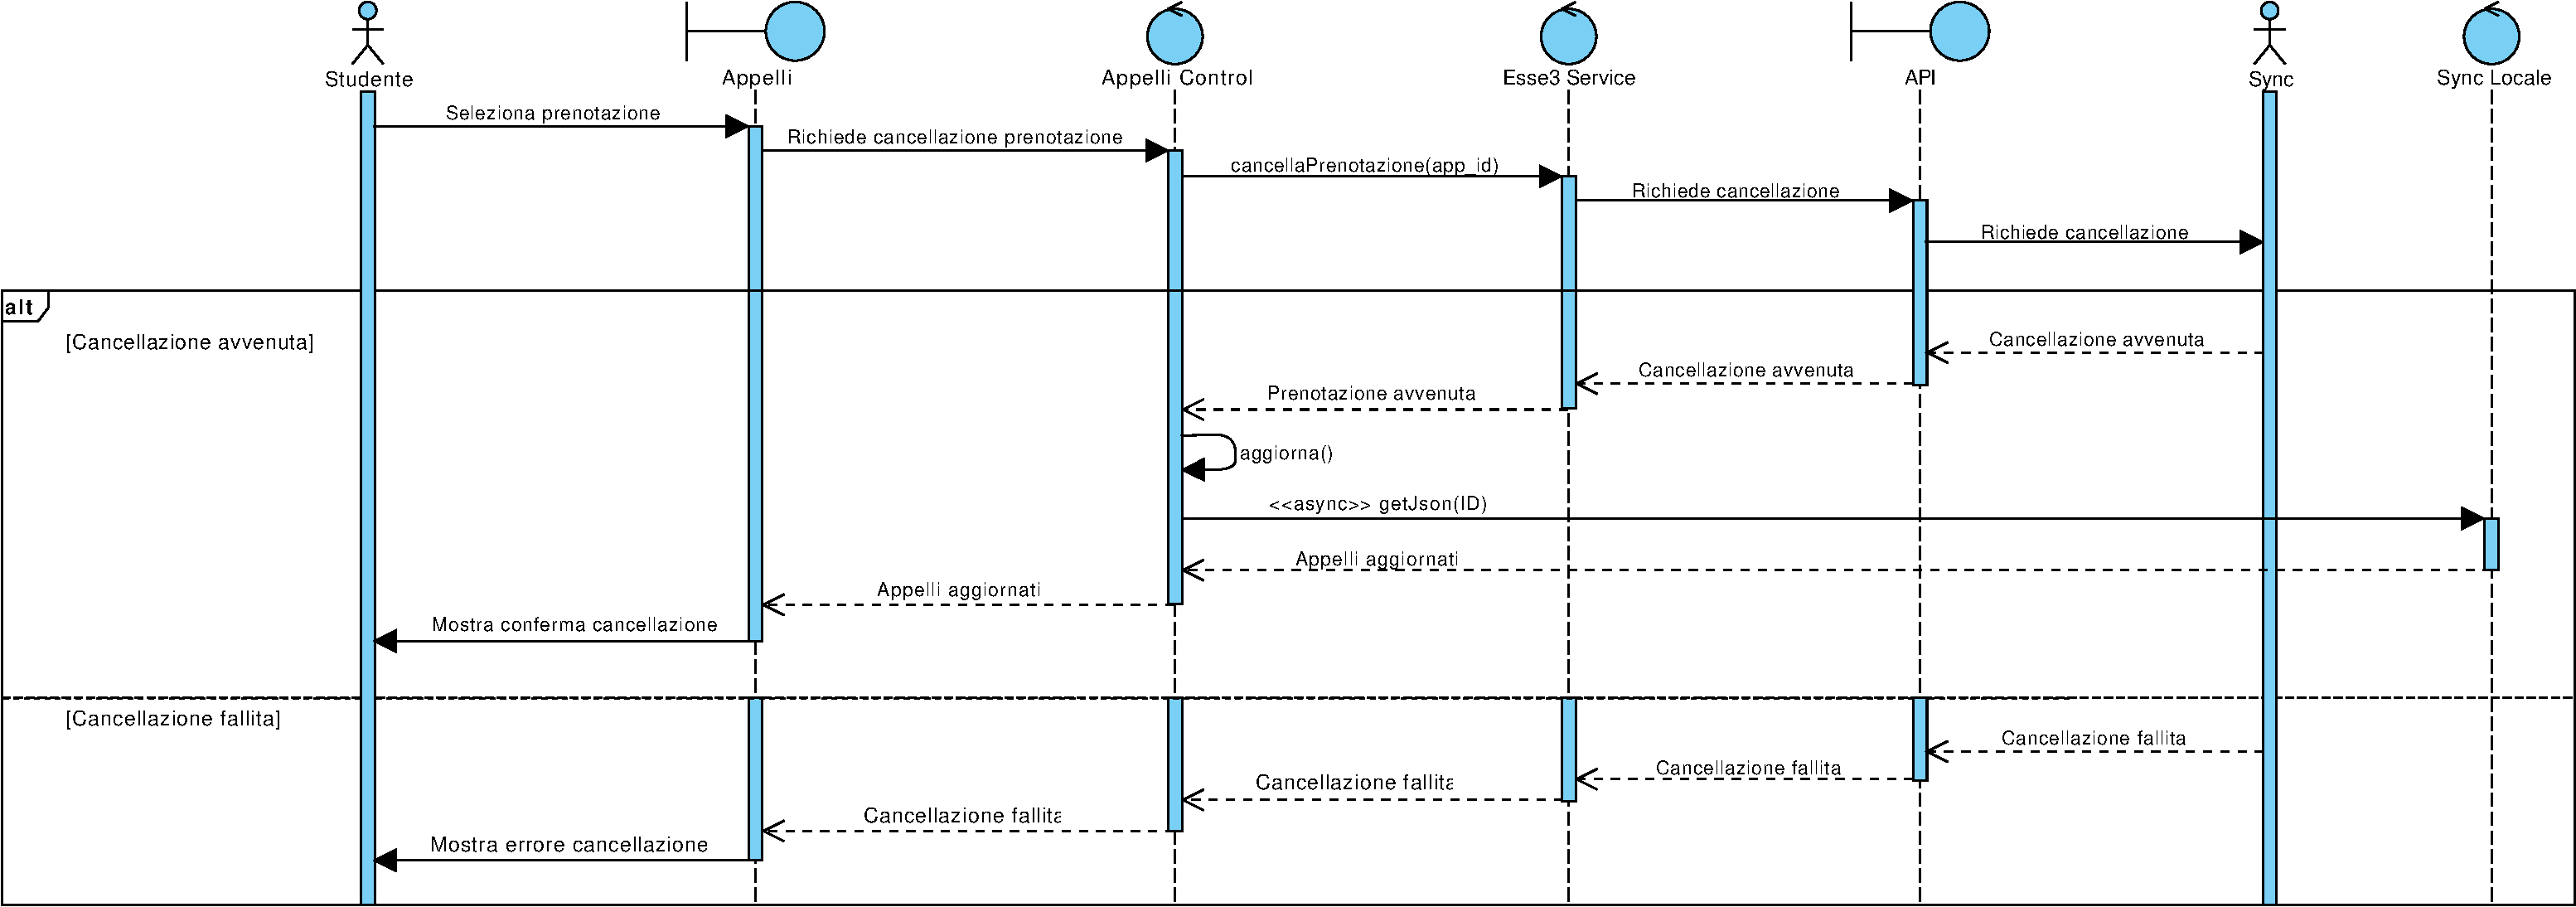
\includegraphics[width=6.5in]{imgs/gruppo1/sequence_diagrams/SD12_cancella_prenotazione.pdf}
\end{center}
\newpage


%%  8.5.13 - Visualizza elenco file  %%
\subsection{Visualizza elenco file}
\begin{center}
	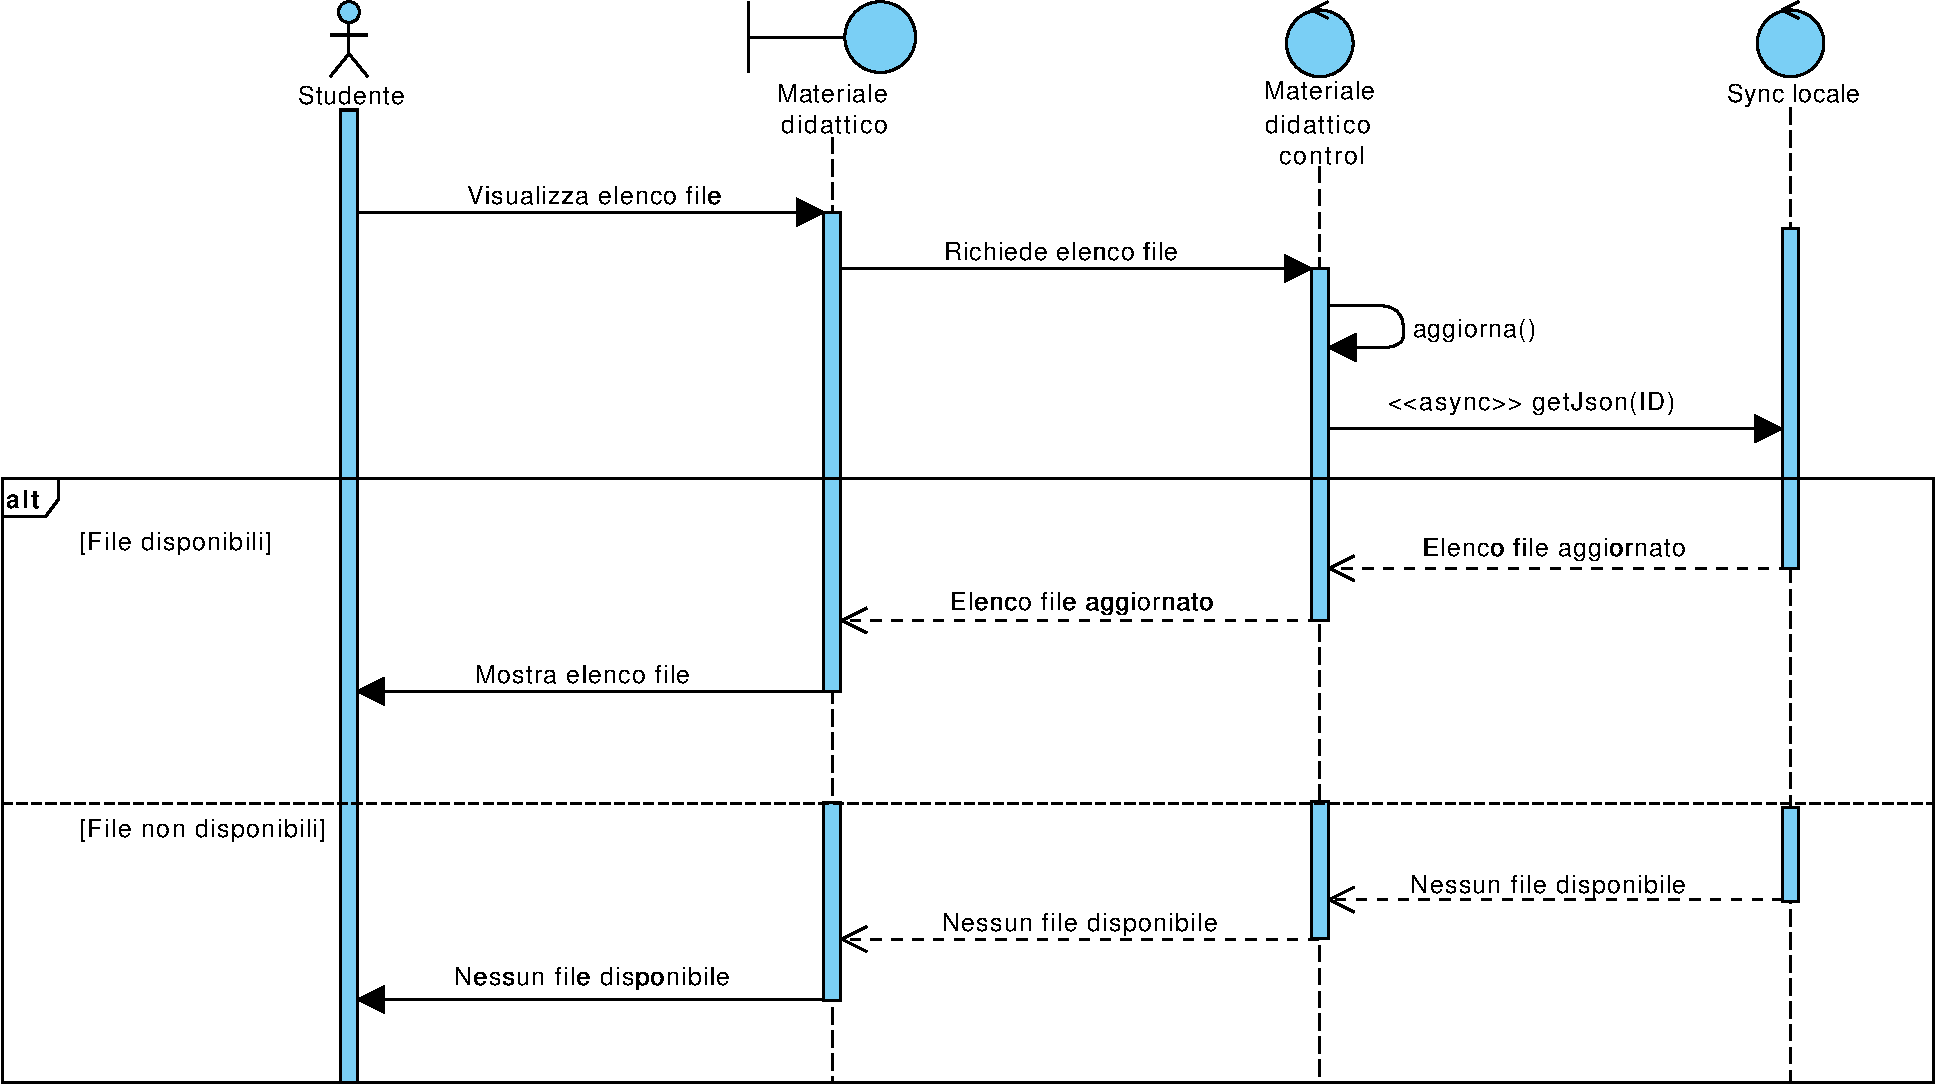
\includegraphics[width=6.5in]{imgs/gruppo1/sequence_diagrams/SD13_visualizza_elenco_file.pdf}
\end{center}
%% 8.5.14 - Ricerca file %
\subsection{Ricerca file}
\begin{center}
	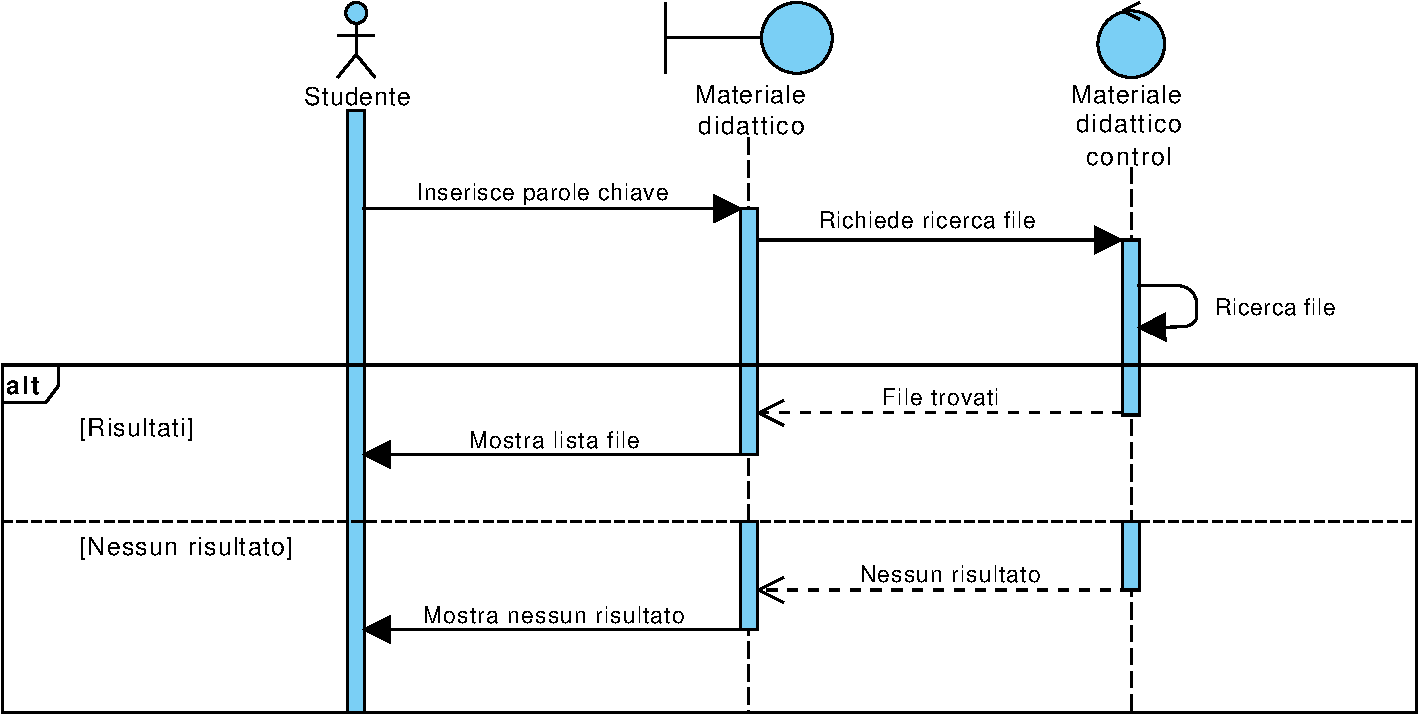
\includegraphics[width=6.5in]{imgs/gruppo1/sequence_diagrams/SD14_ricerca_file.pdf}
\end{center}
\newpage


%% 8.5.15 - Visualizza dettagli file %%
\subsection{Visualizza dettagli file}
\begin{center}
	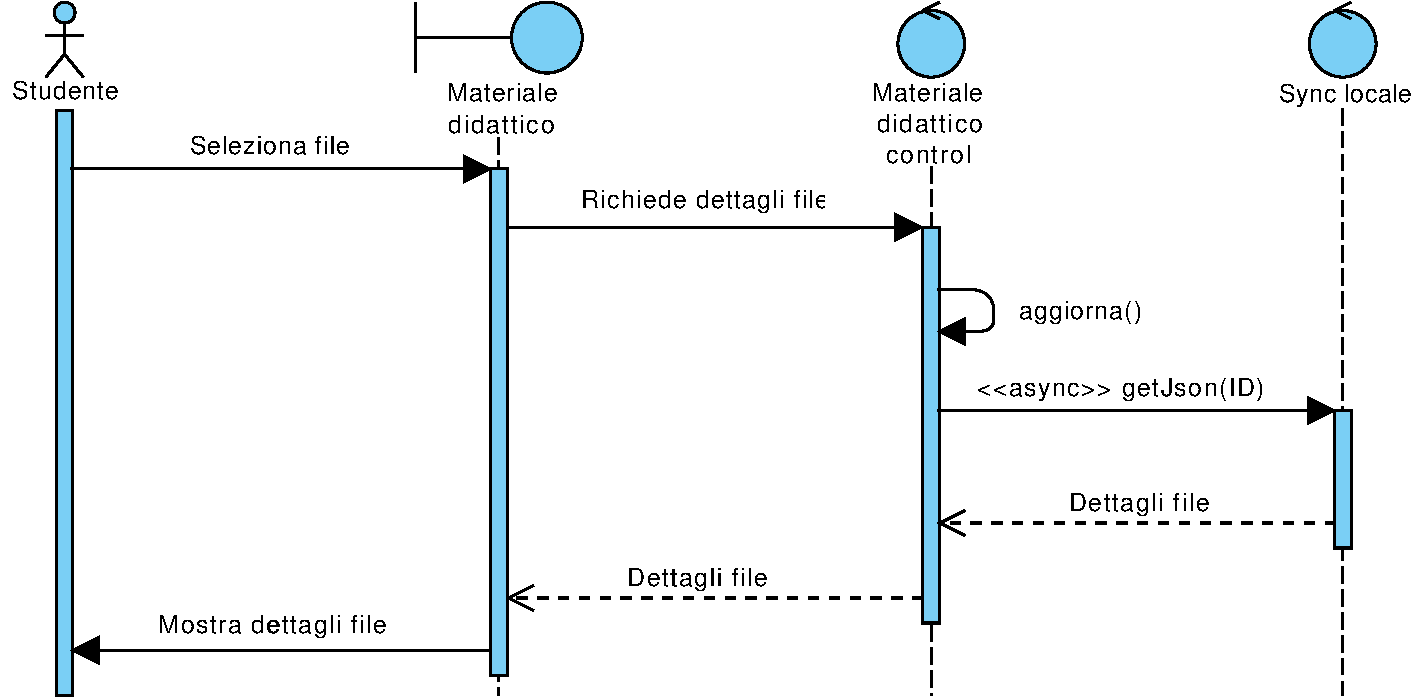
\includegraphics[width=6.5in]{imgs/gruppo1//sequence_diagrams/SD15_visualizza_dettagli_file.pdf}
\end{center}
%% 8.5.16- Apri file  %%
\subsection{Apri file}
\begin{center}
	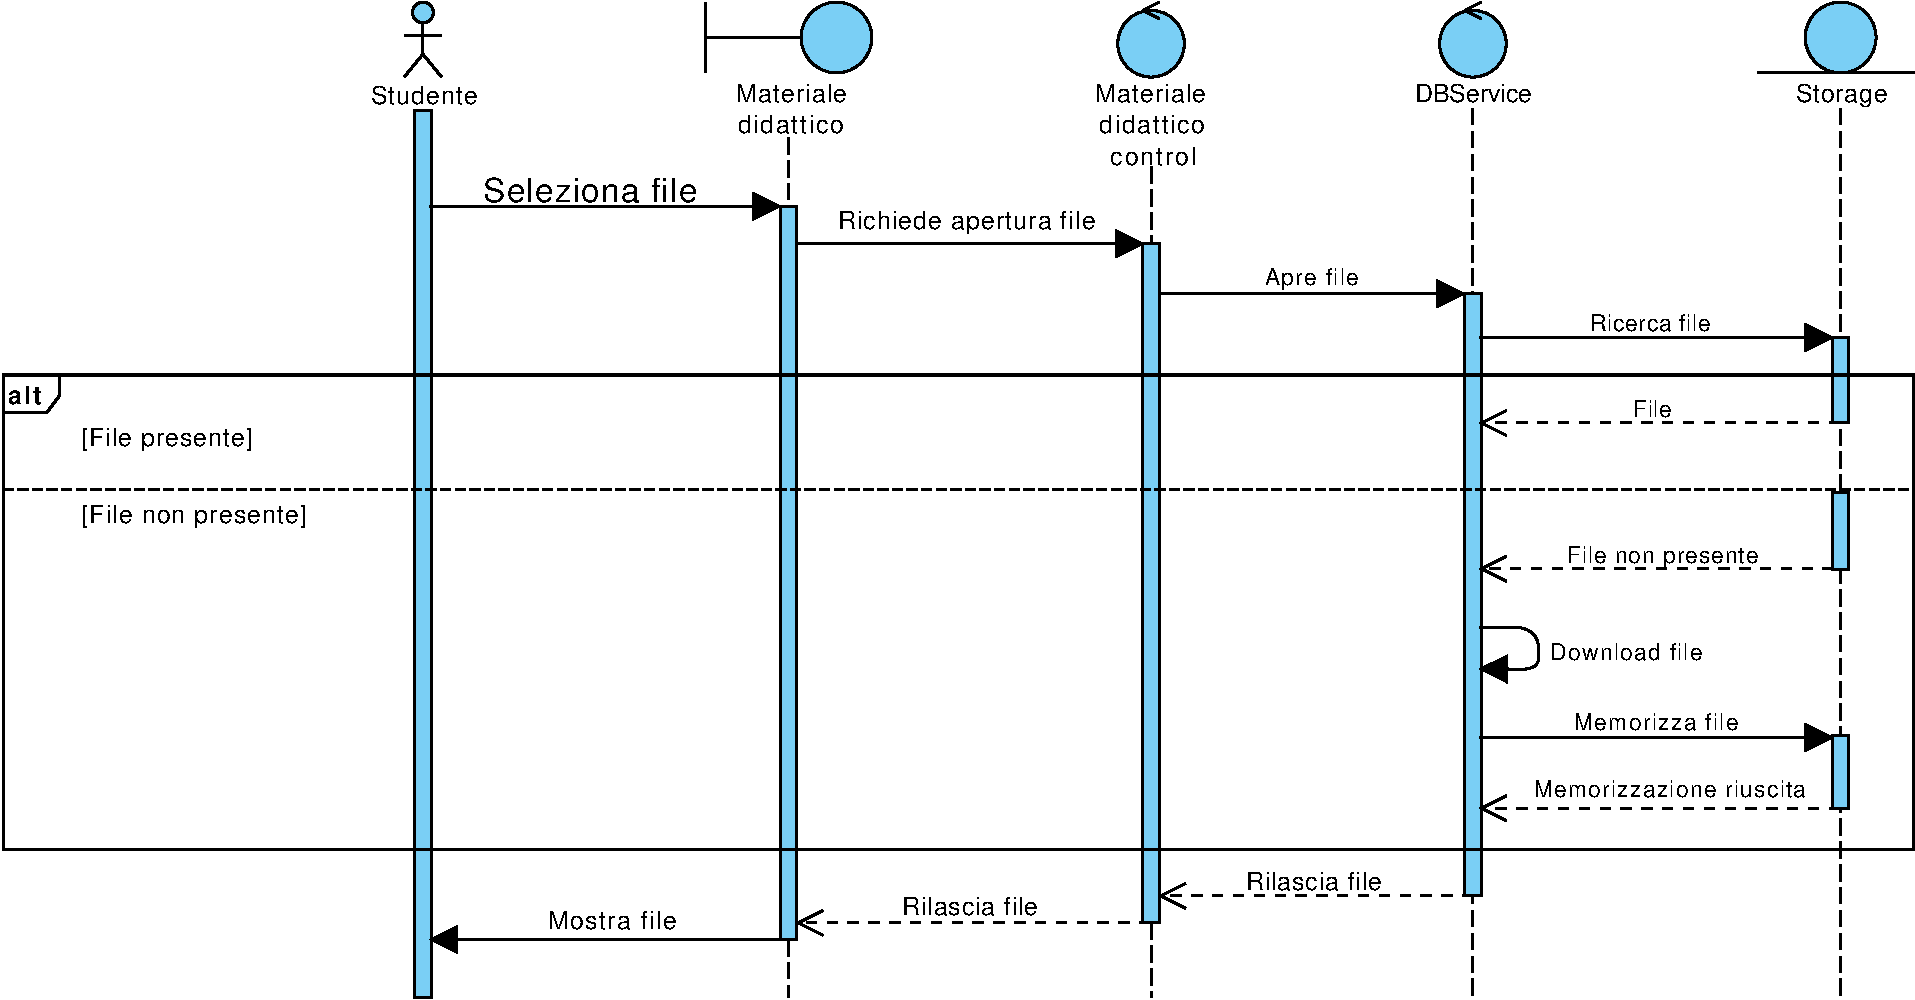
\includegraphics[width=6.5in]{imgs/gruppo1/sequence_diagrams/SD16_apri_file.pdf}
\end{center}
\newpage


%% 8.5.17 - Rimuovi file %%
\subsection{Rimuovi  file}
\begin{center}
	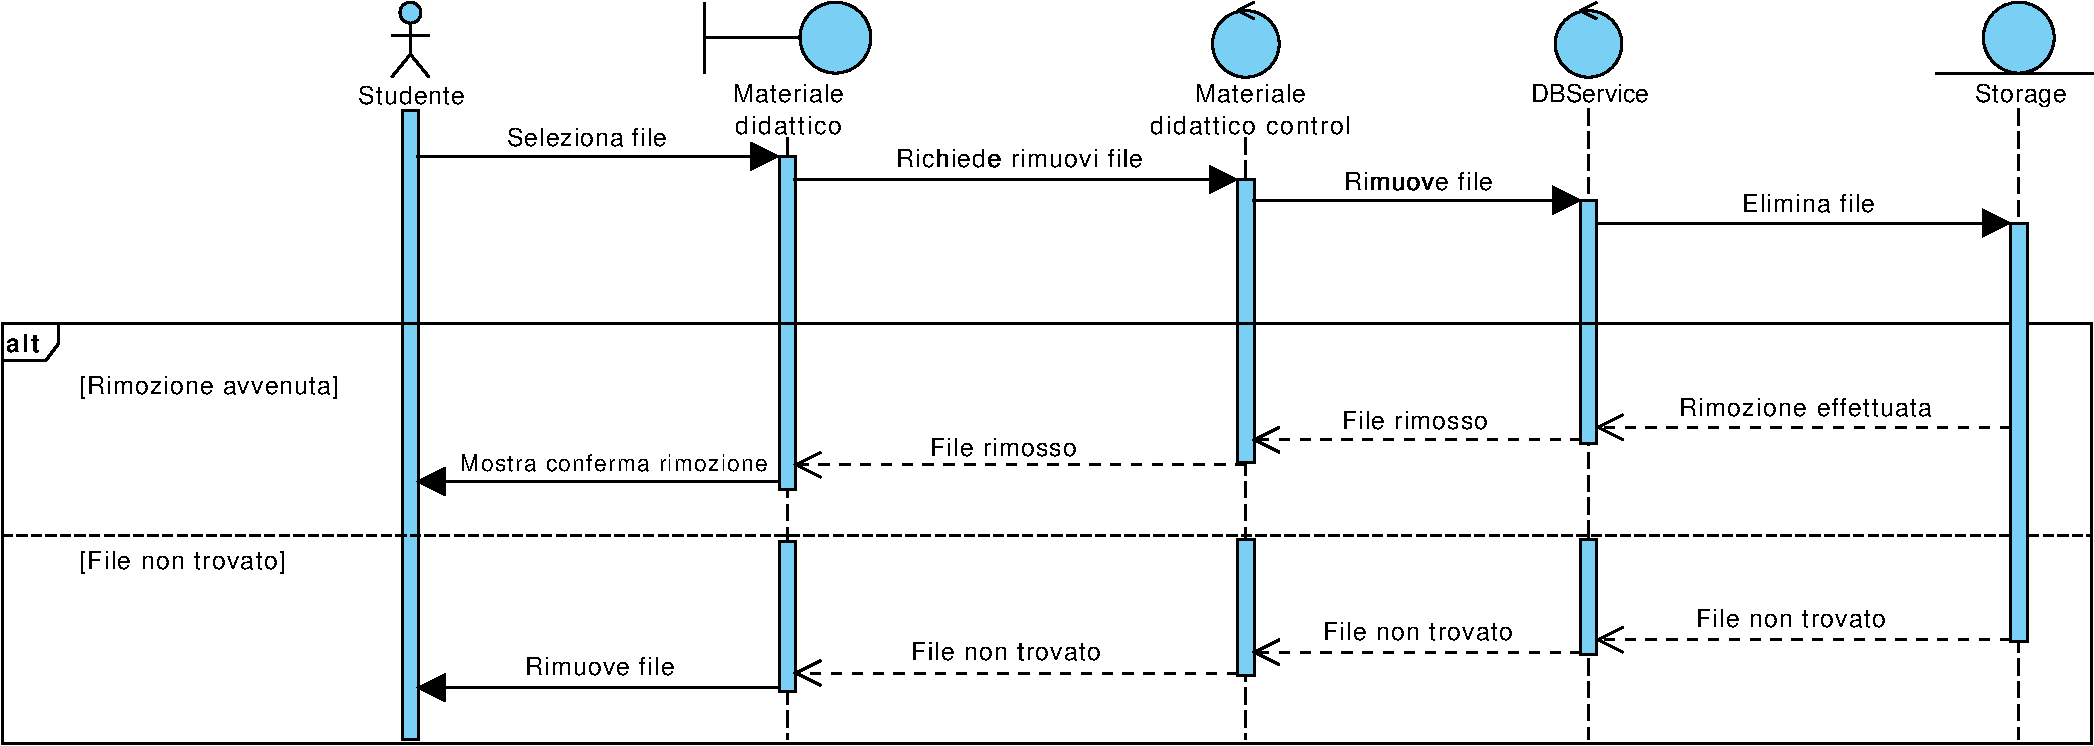
\includegraphics[width=6.5in]{imgs/gruppo1/sequence_diagrams/SD17_rimuovi_file.pdf}
\end{center}
\newpage




\section{Diagrammi delle attività}

%% 8.6.1 - Visualizza corsi %%
\subsection{Visualizza corsi}
\begin{center}
	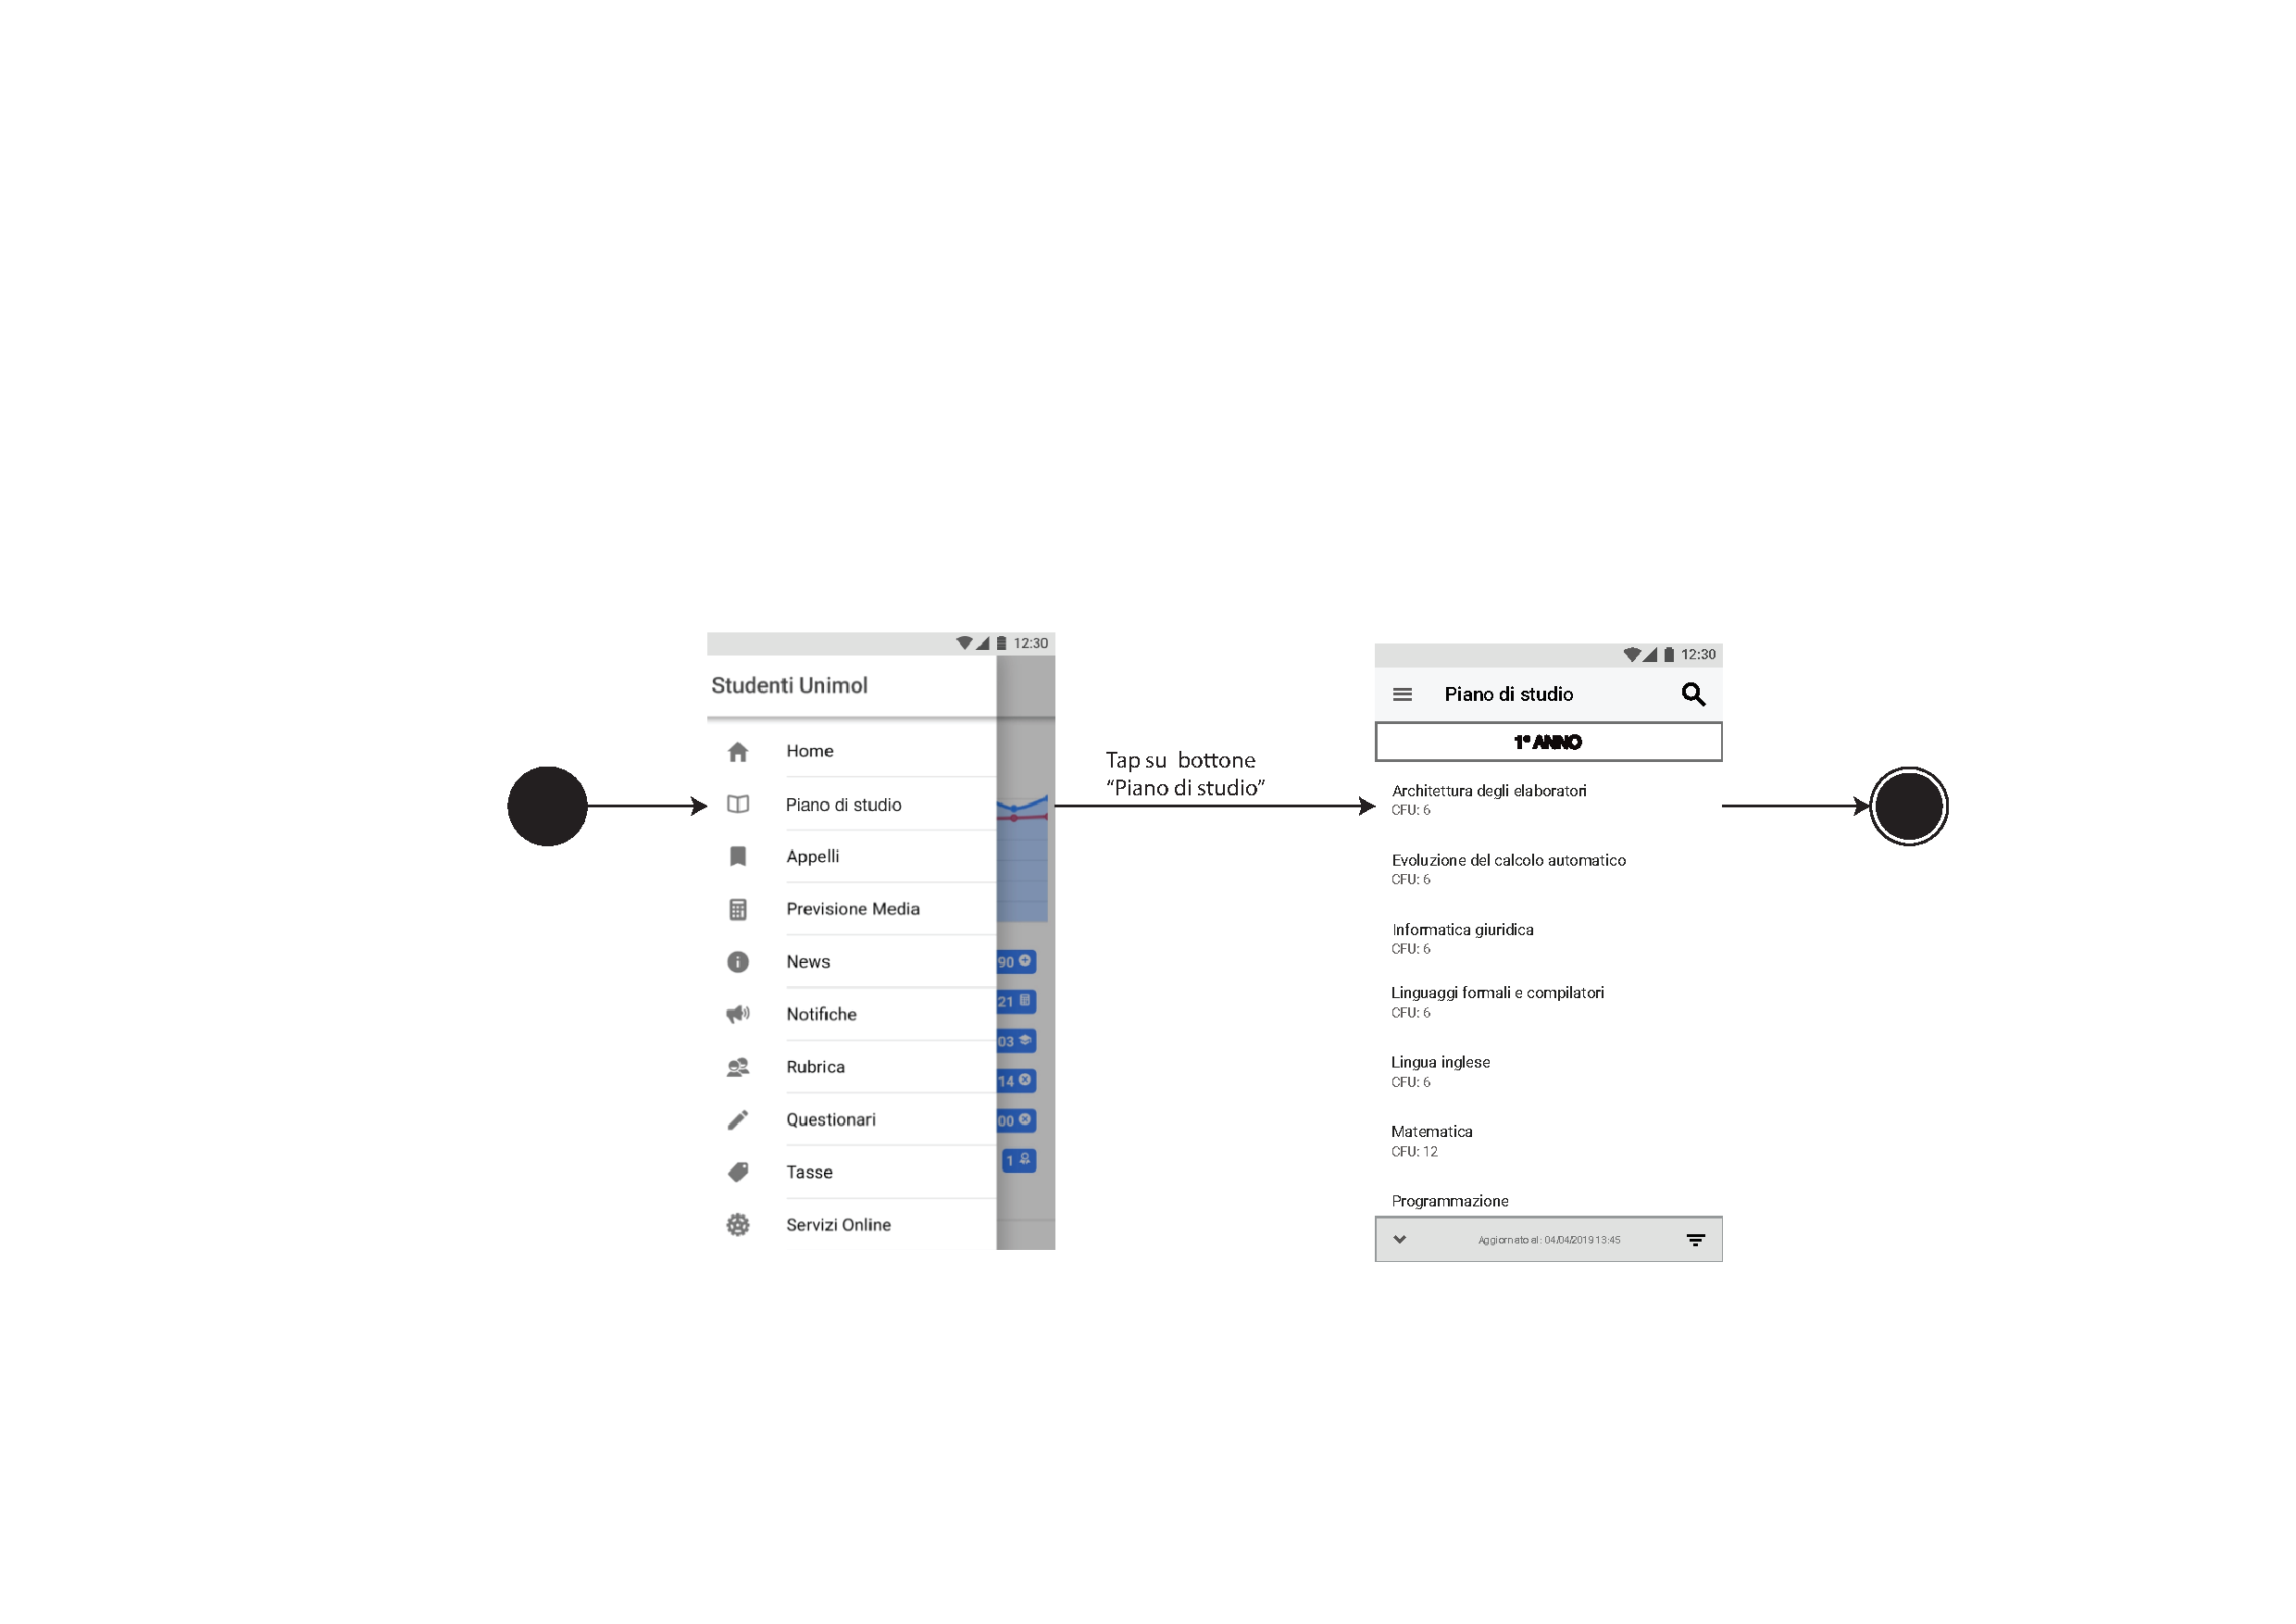
\includegraphics[width=6in]{imgs/gruppo1/activity_diagrams/AD1_Visualizza_corsi.pdf}
\end{center}
\newpage

%%8.6.2 - Ricerca corsi  %%

\subsection{Ricerca corsi }
\begin{center}
	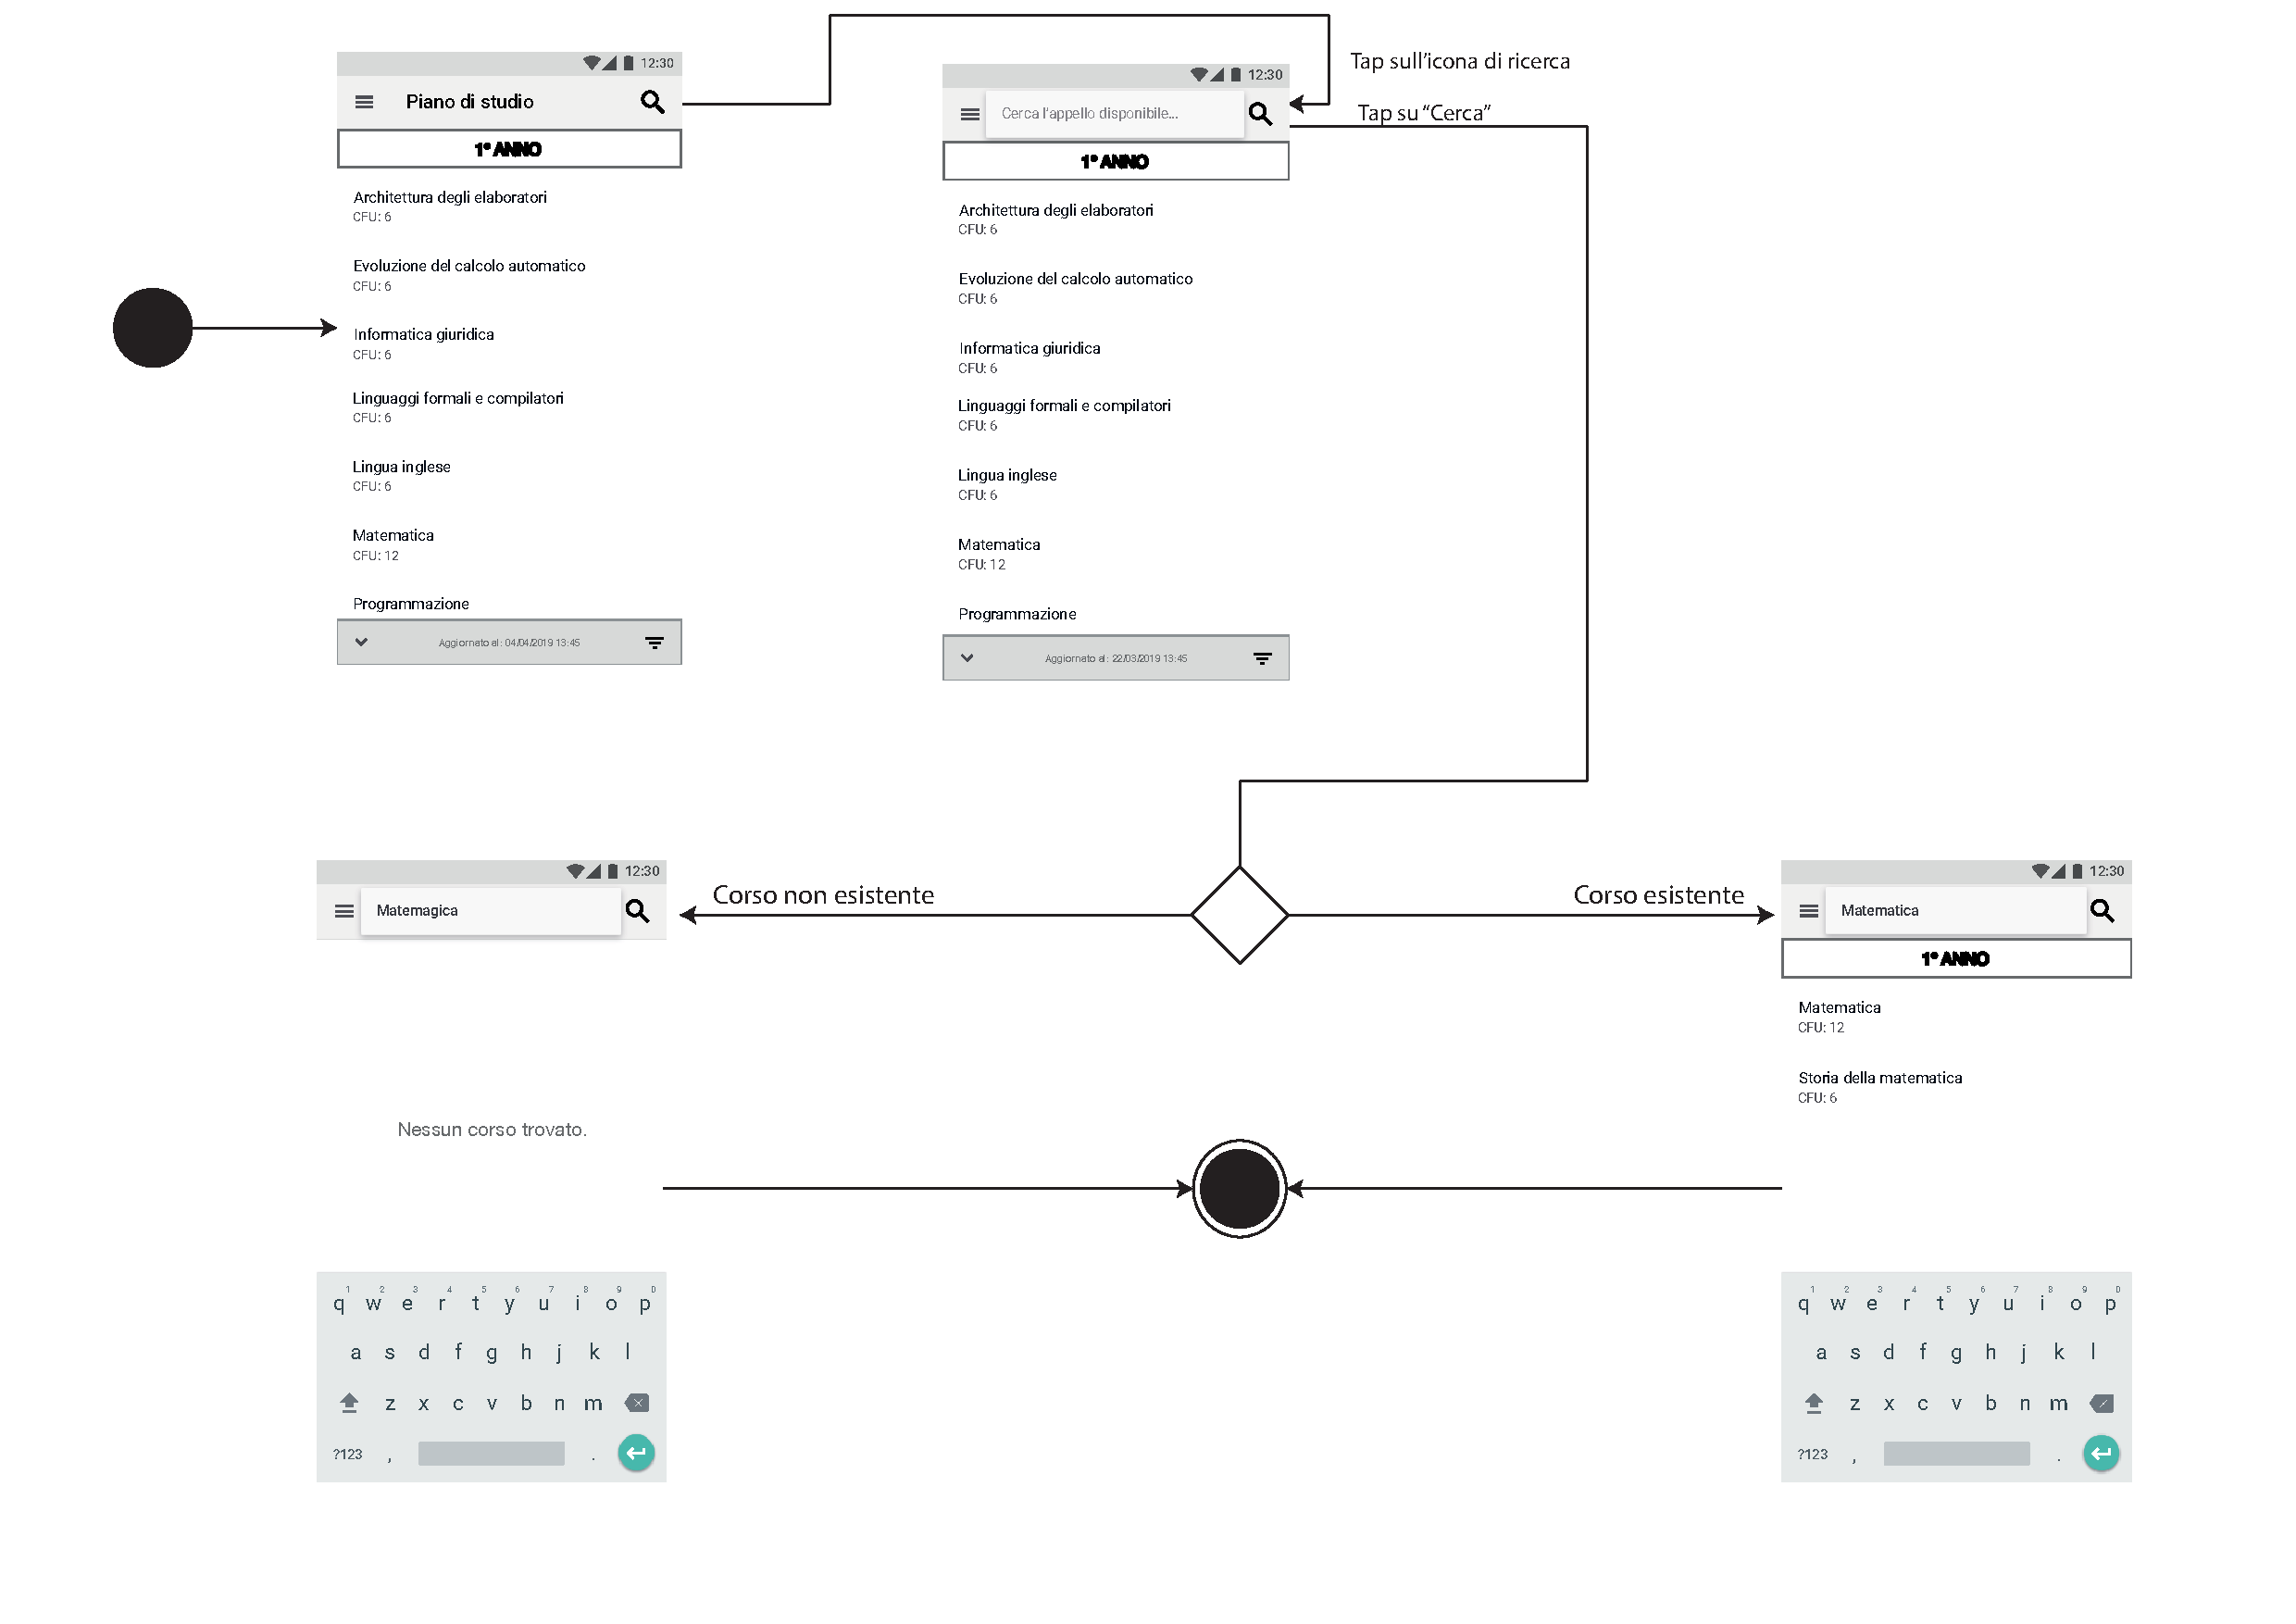
\includegraphics[width=6in]{imgs/gruppo1/activity_diagrams/AD2_ricerca_corsi.pdf}
\end{center}
\newpage

%%8.6.3 - Filtra corsi con memorizzazione %%

\subsection{Filtra corsi con memorizzazione  }
\begin{center}
	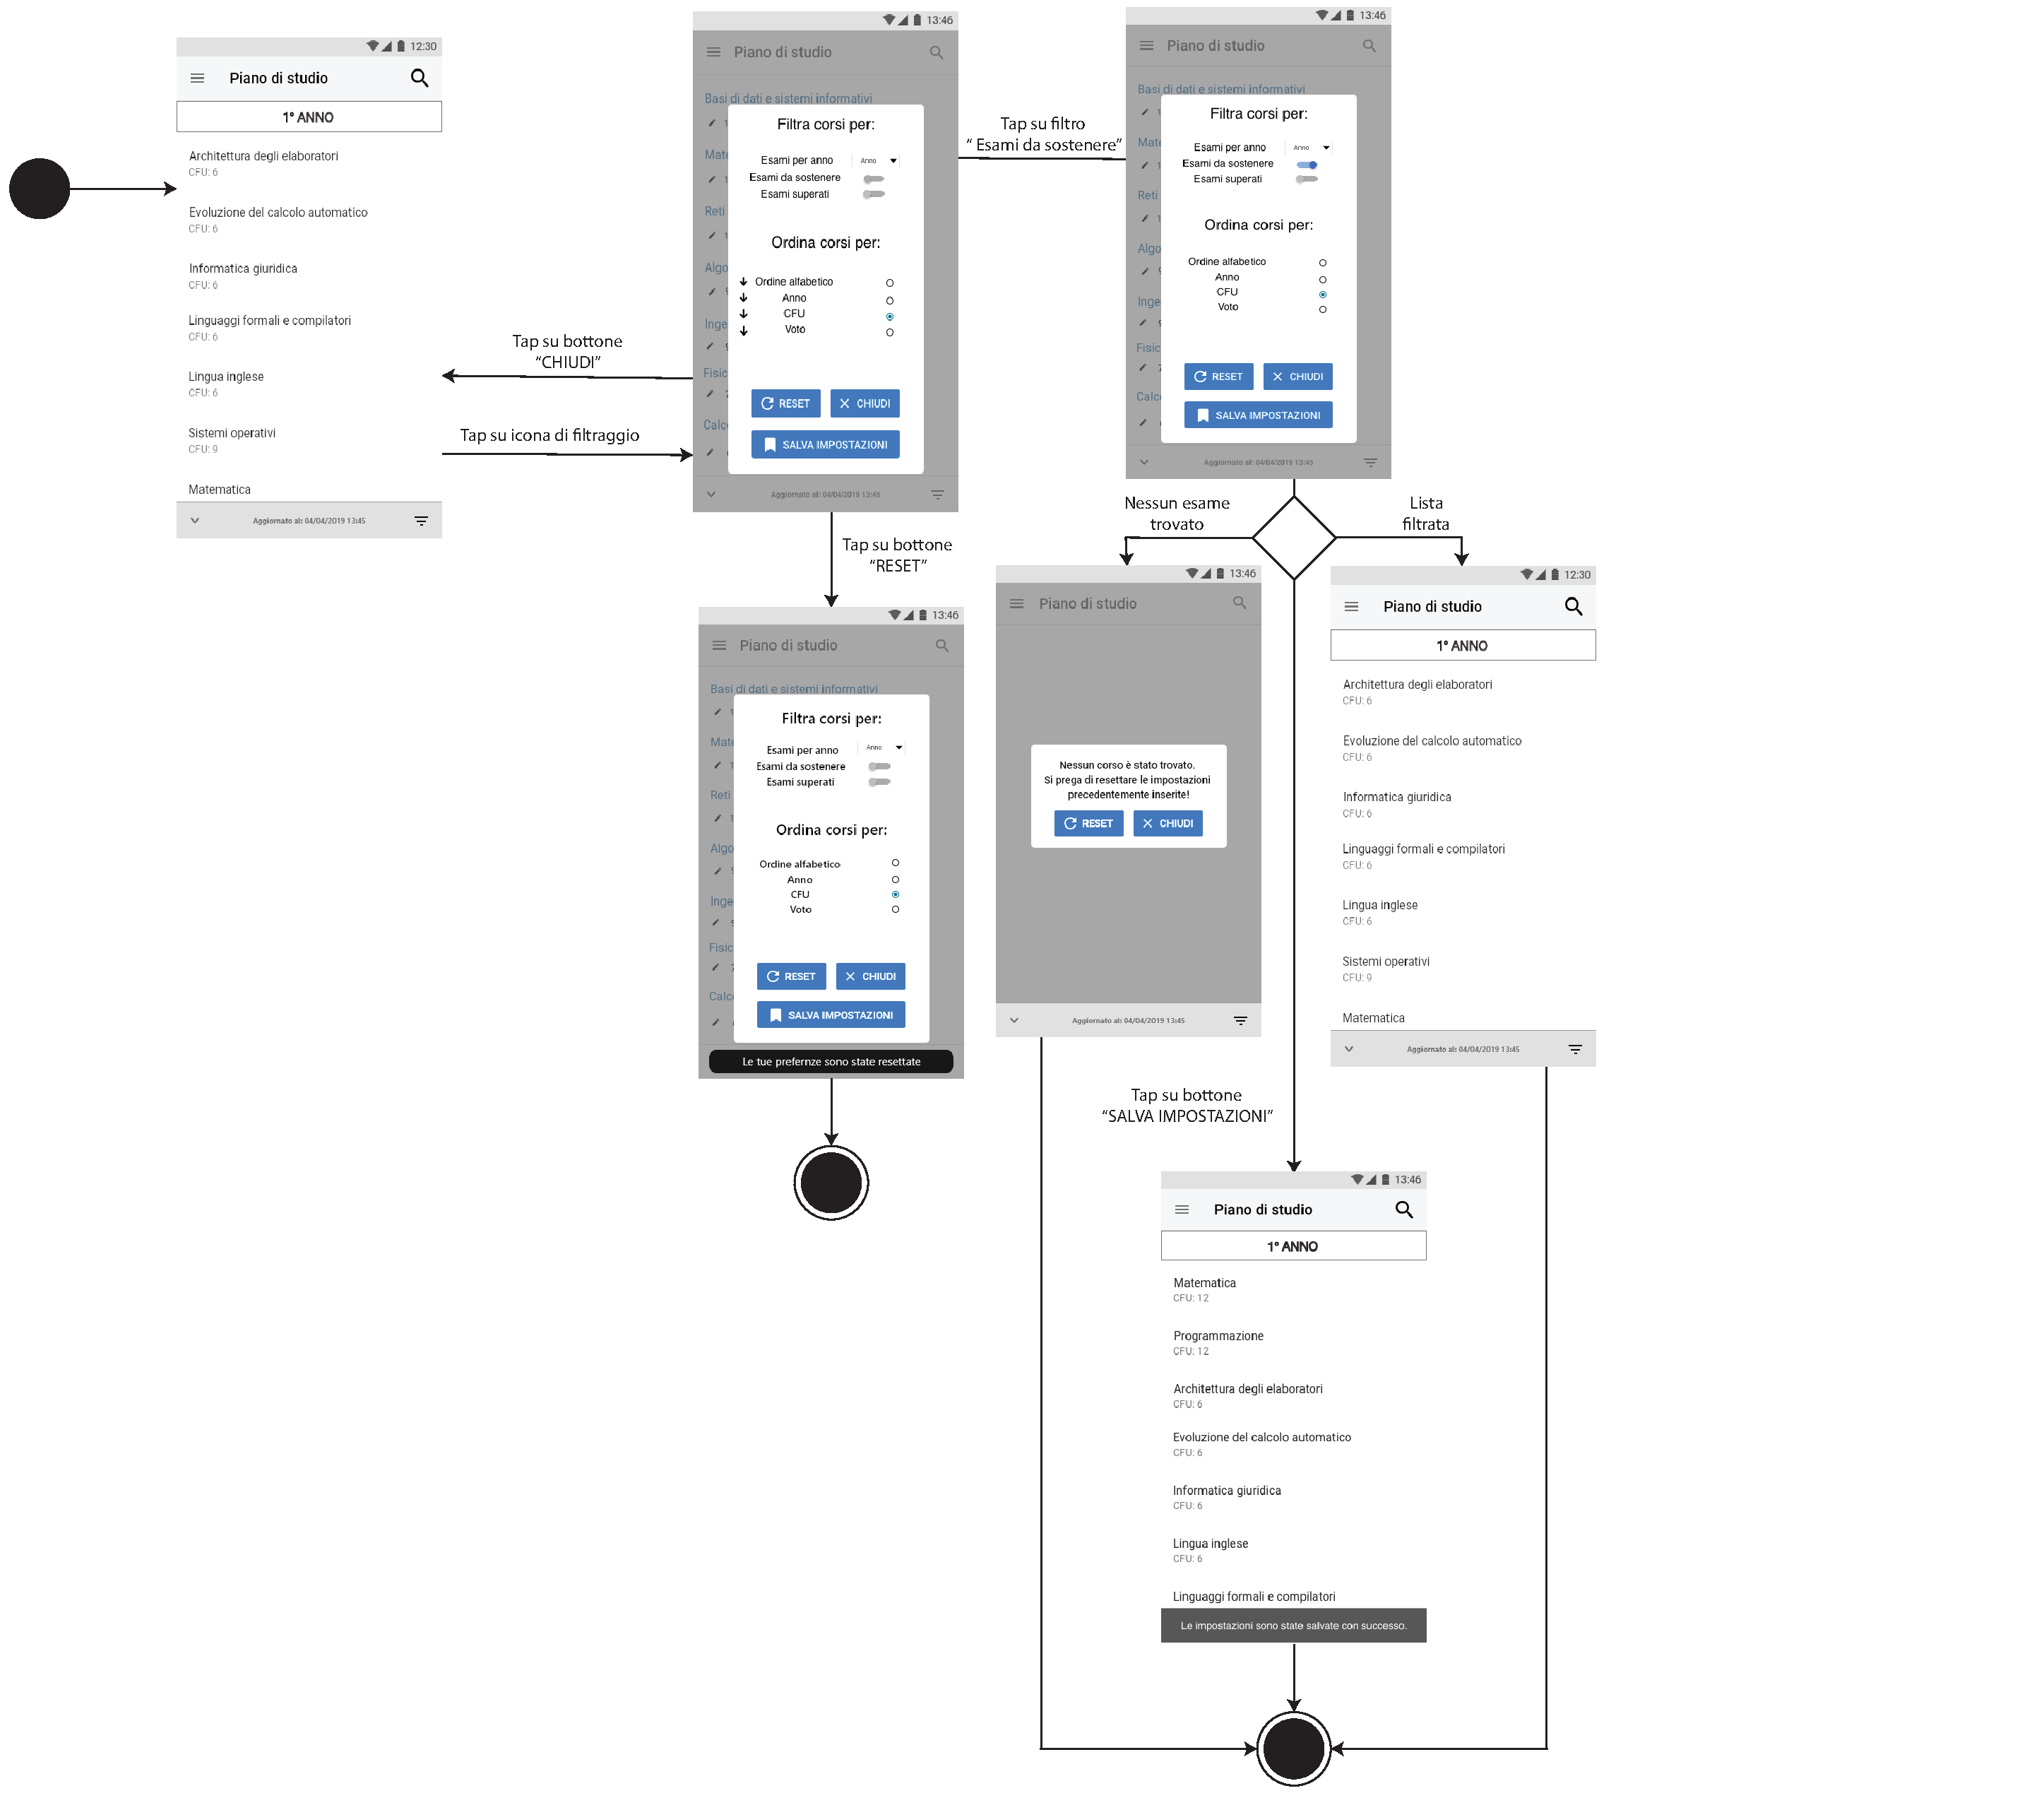
\includegraphics[width=6in]{imgs/gruppo1/activity_diagrams/AD3_filtra_corsi.pdf}
\end{center}
\newpage

%%8.6.4 - Ordina corsi con memorizzazione %%

\subsection{Ordina corsi con memorizzazione}
\begin{center}
	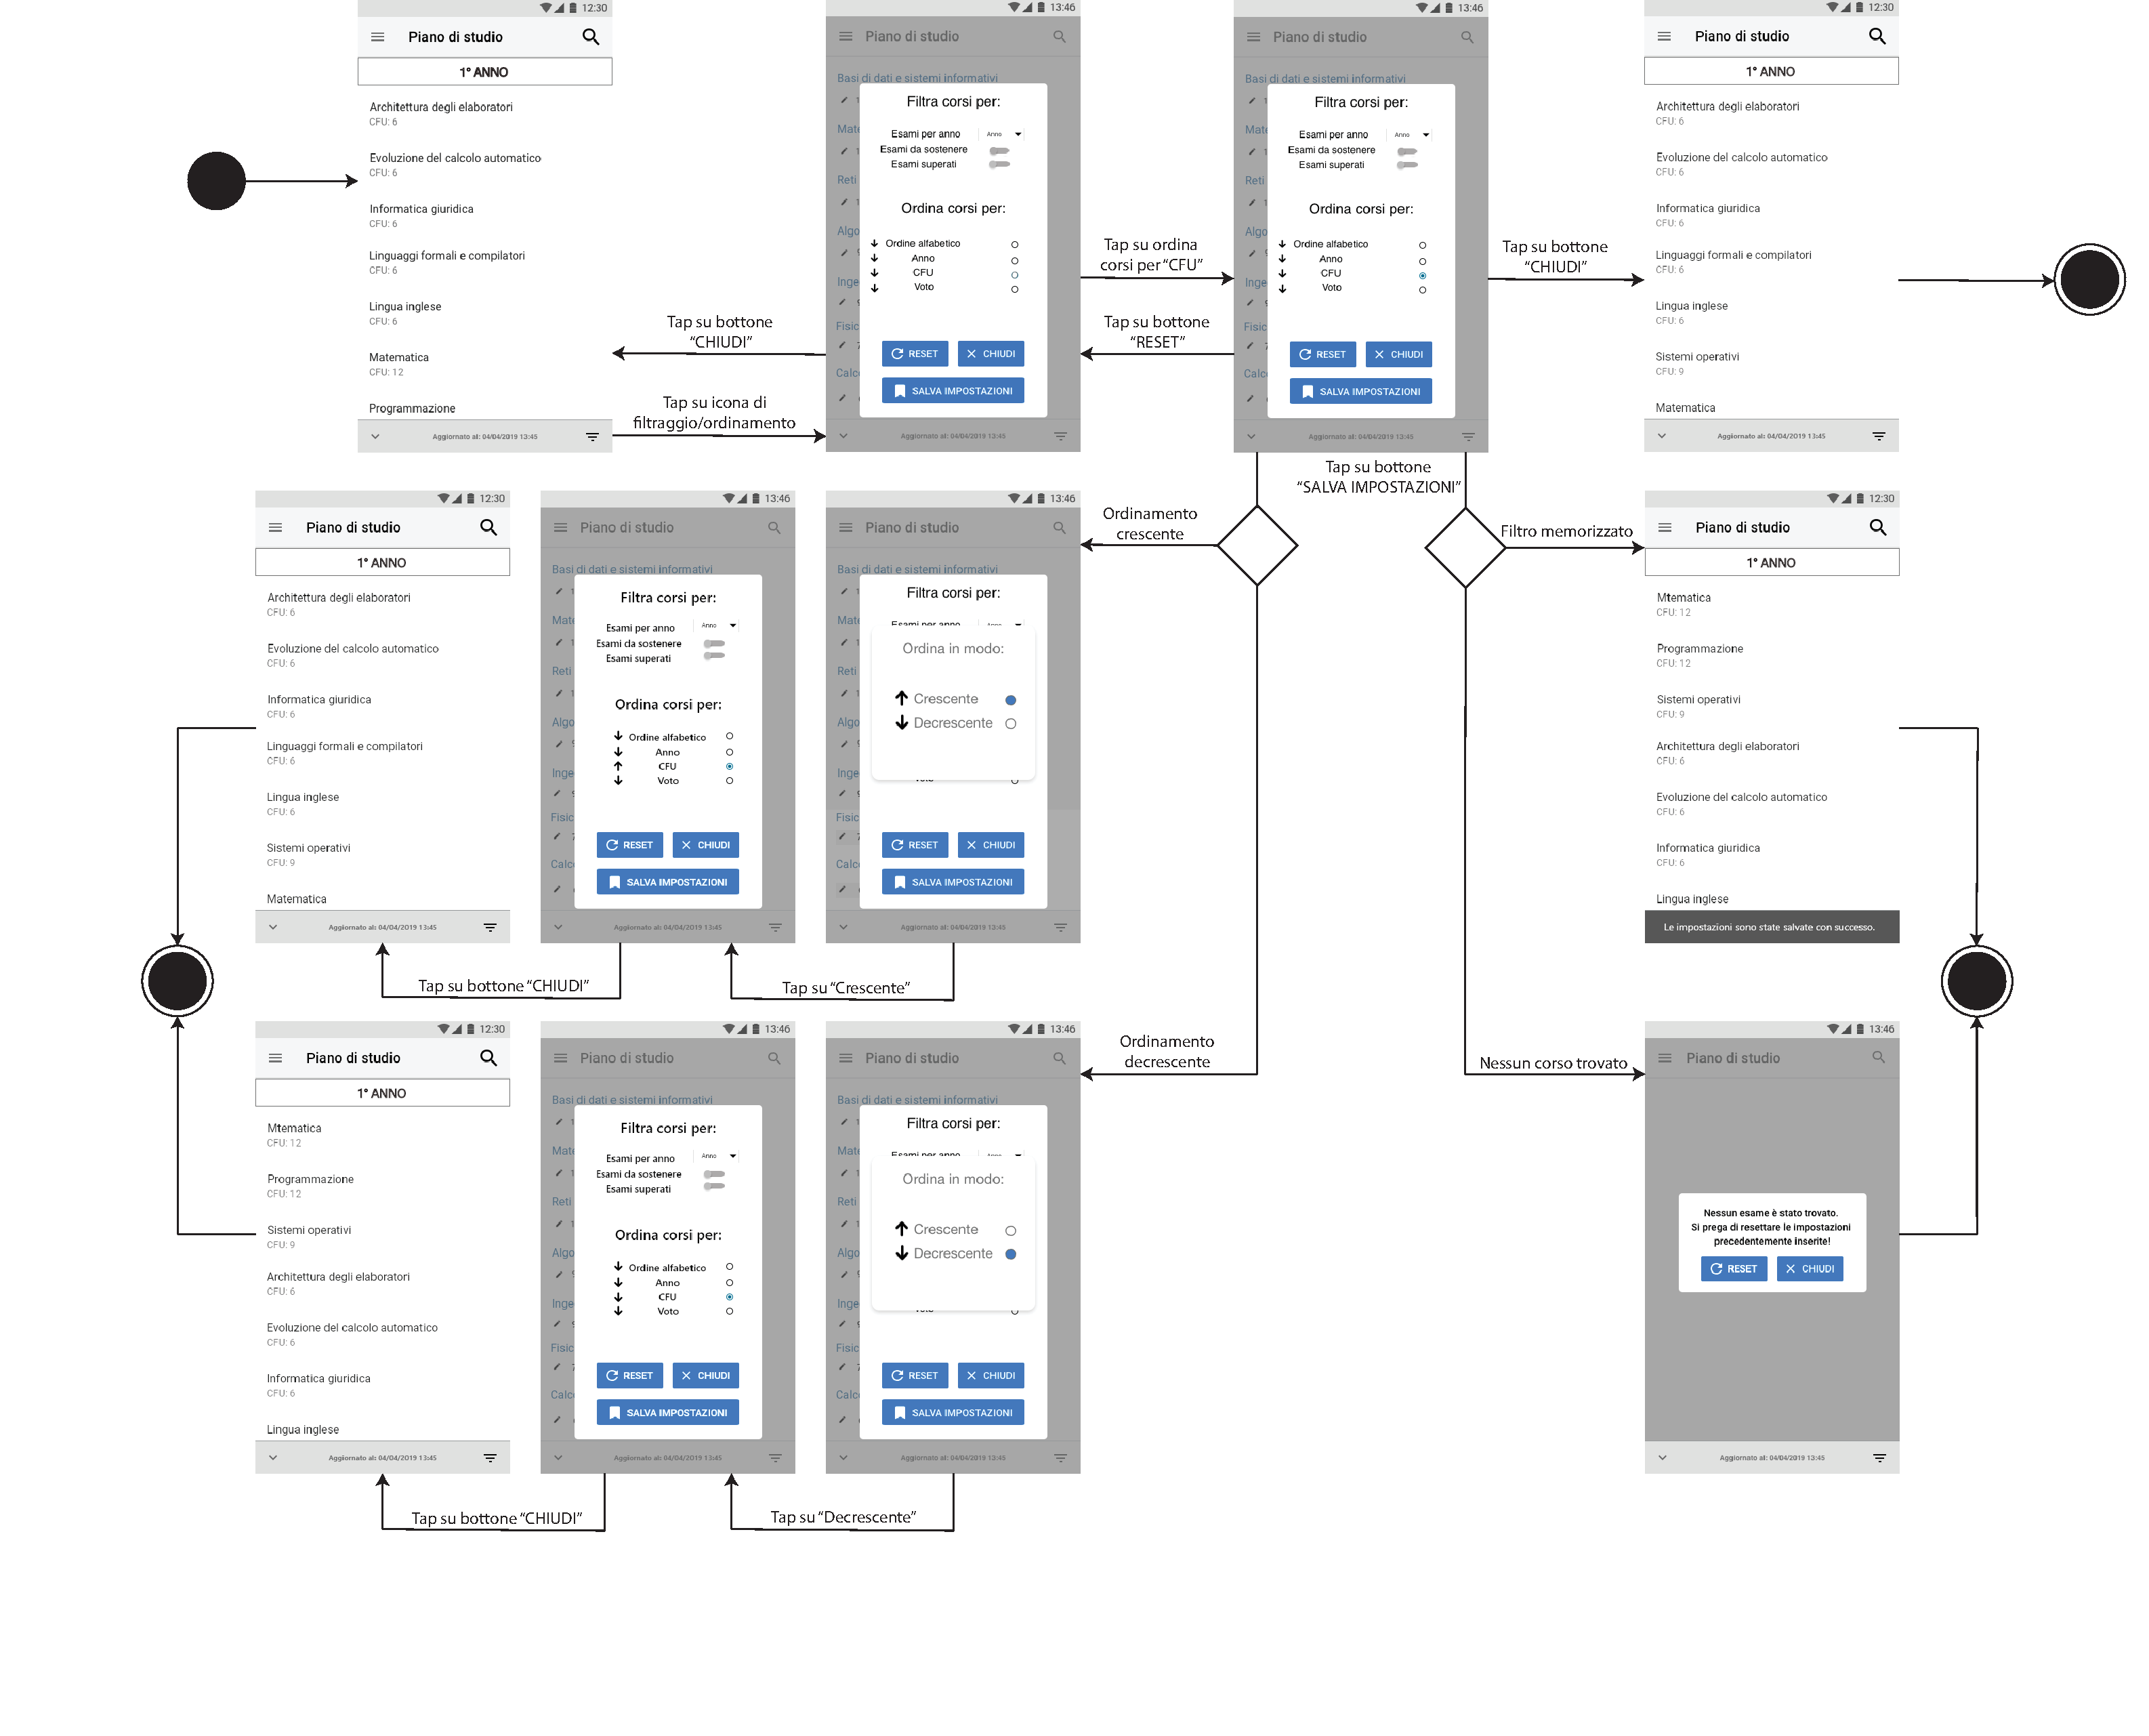
\includegraphics[width=6in]{imgs/gruppo1/activity_diagrams/AD4_ordina_corsi.pdf}
\end{center}
\newpage

%%8.6.5 - Visualizza dettagli corso%%

\subsection{Visualizza dettagli corso}
\begin{center}
	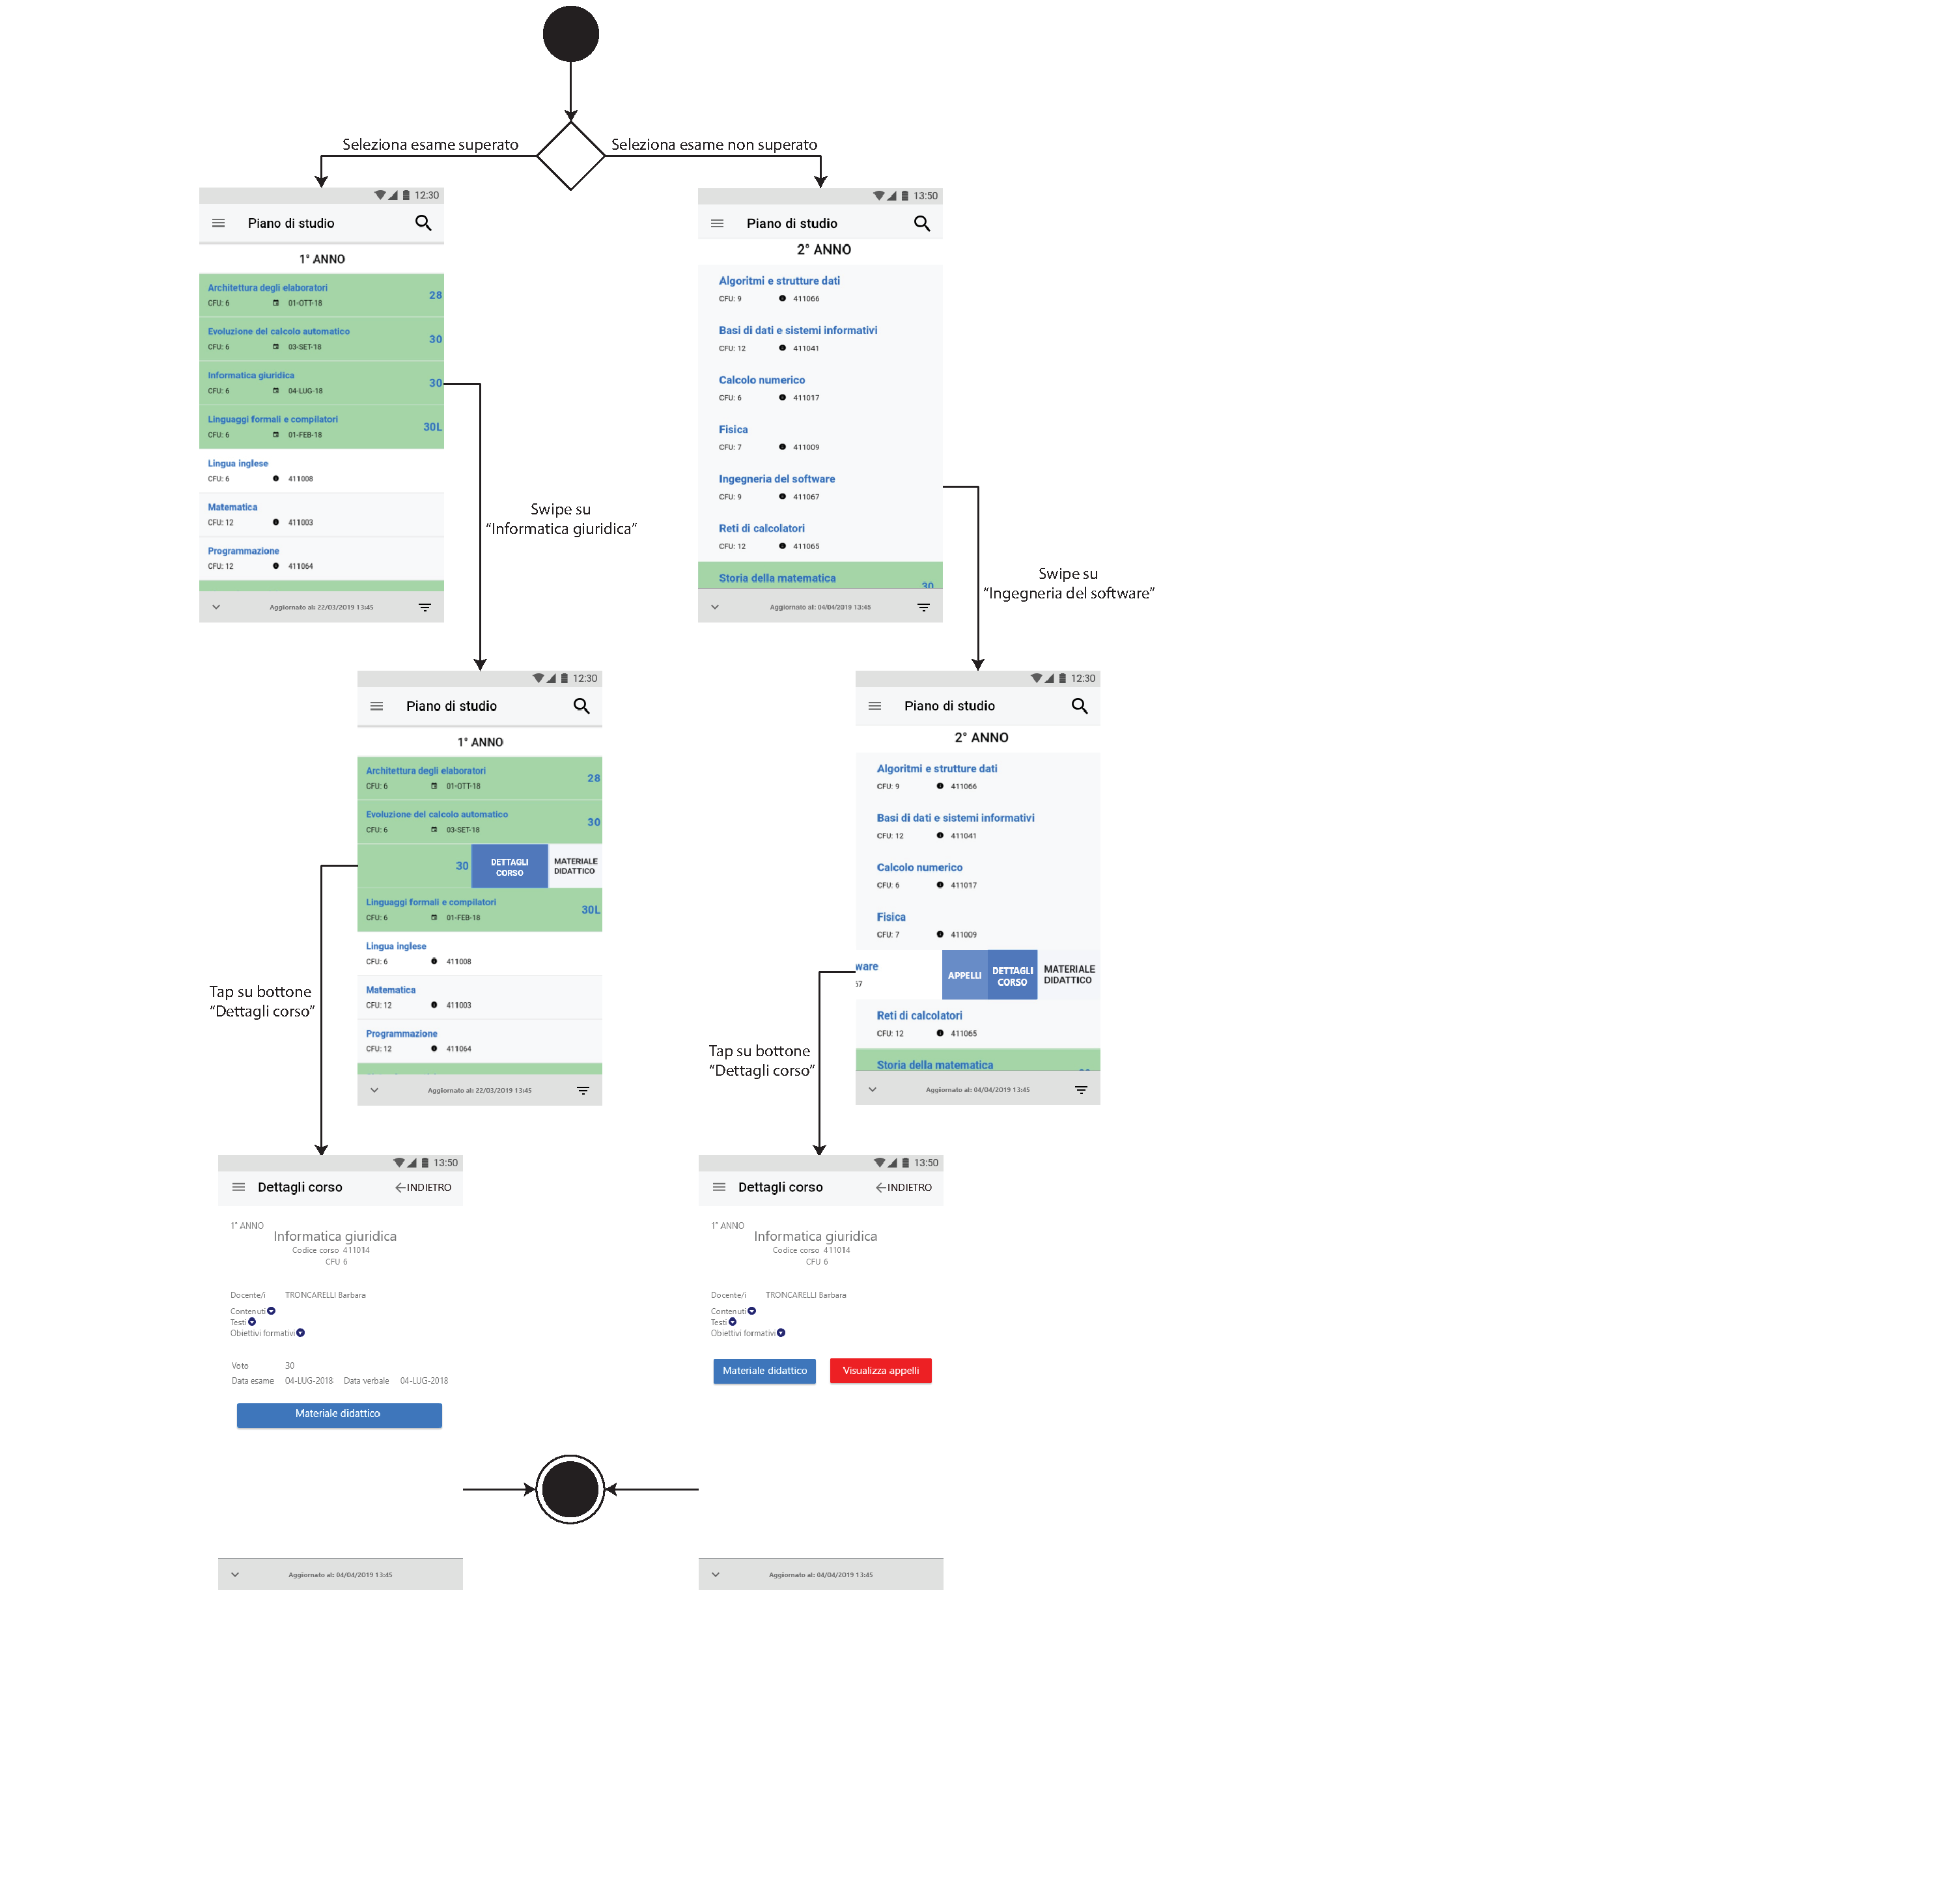
\includegraphics[width=7in]{imgs/gruppo1/activity_diagrams/AD5_visualizza_dettagli_corso.pdf}
\end{center}
\newpage

%%8.6.6 - Visualizza appelli disponibili%%

\subsection{Visualizza appelli disponibil}
\begin{center}
	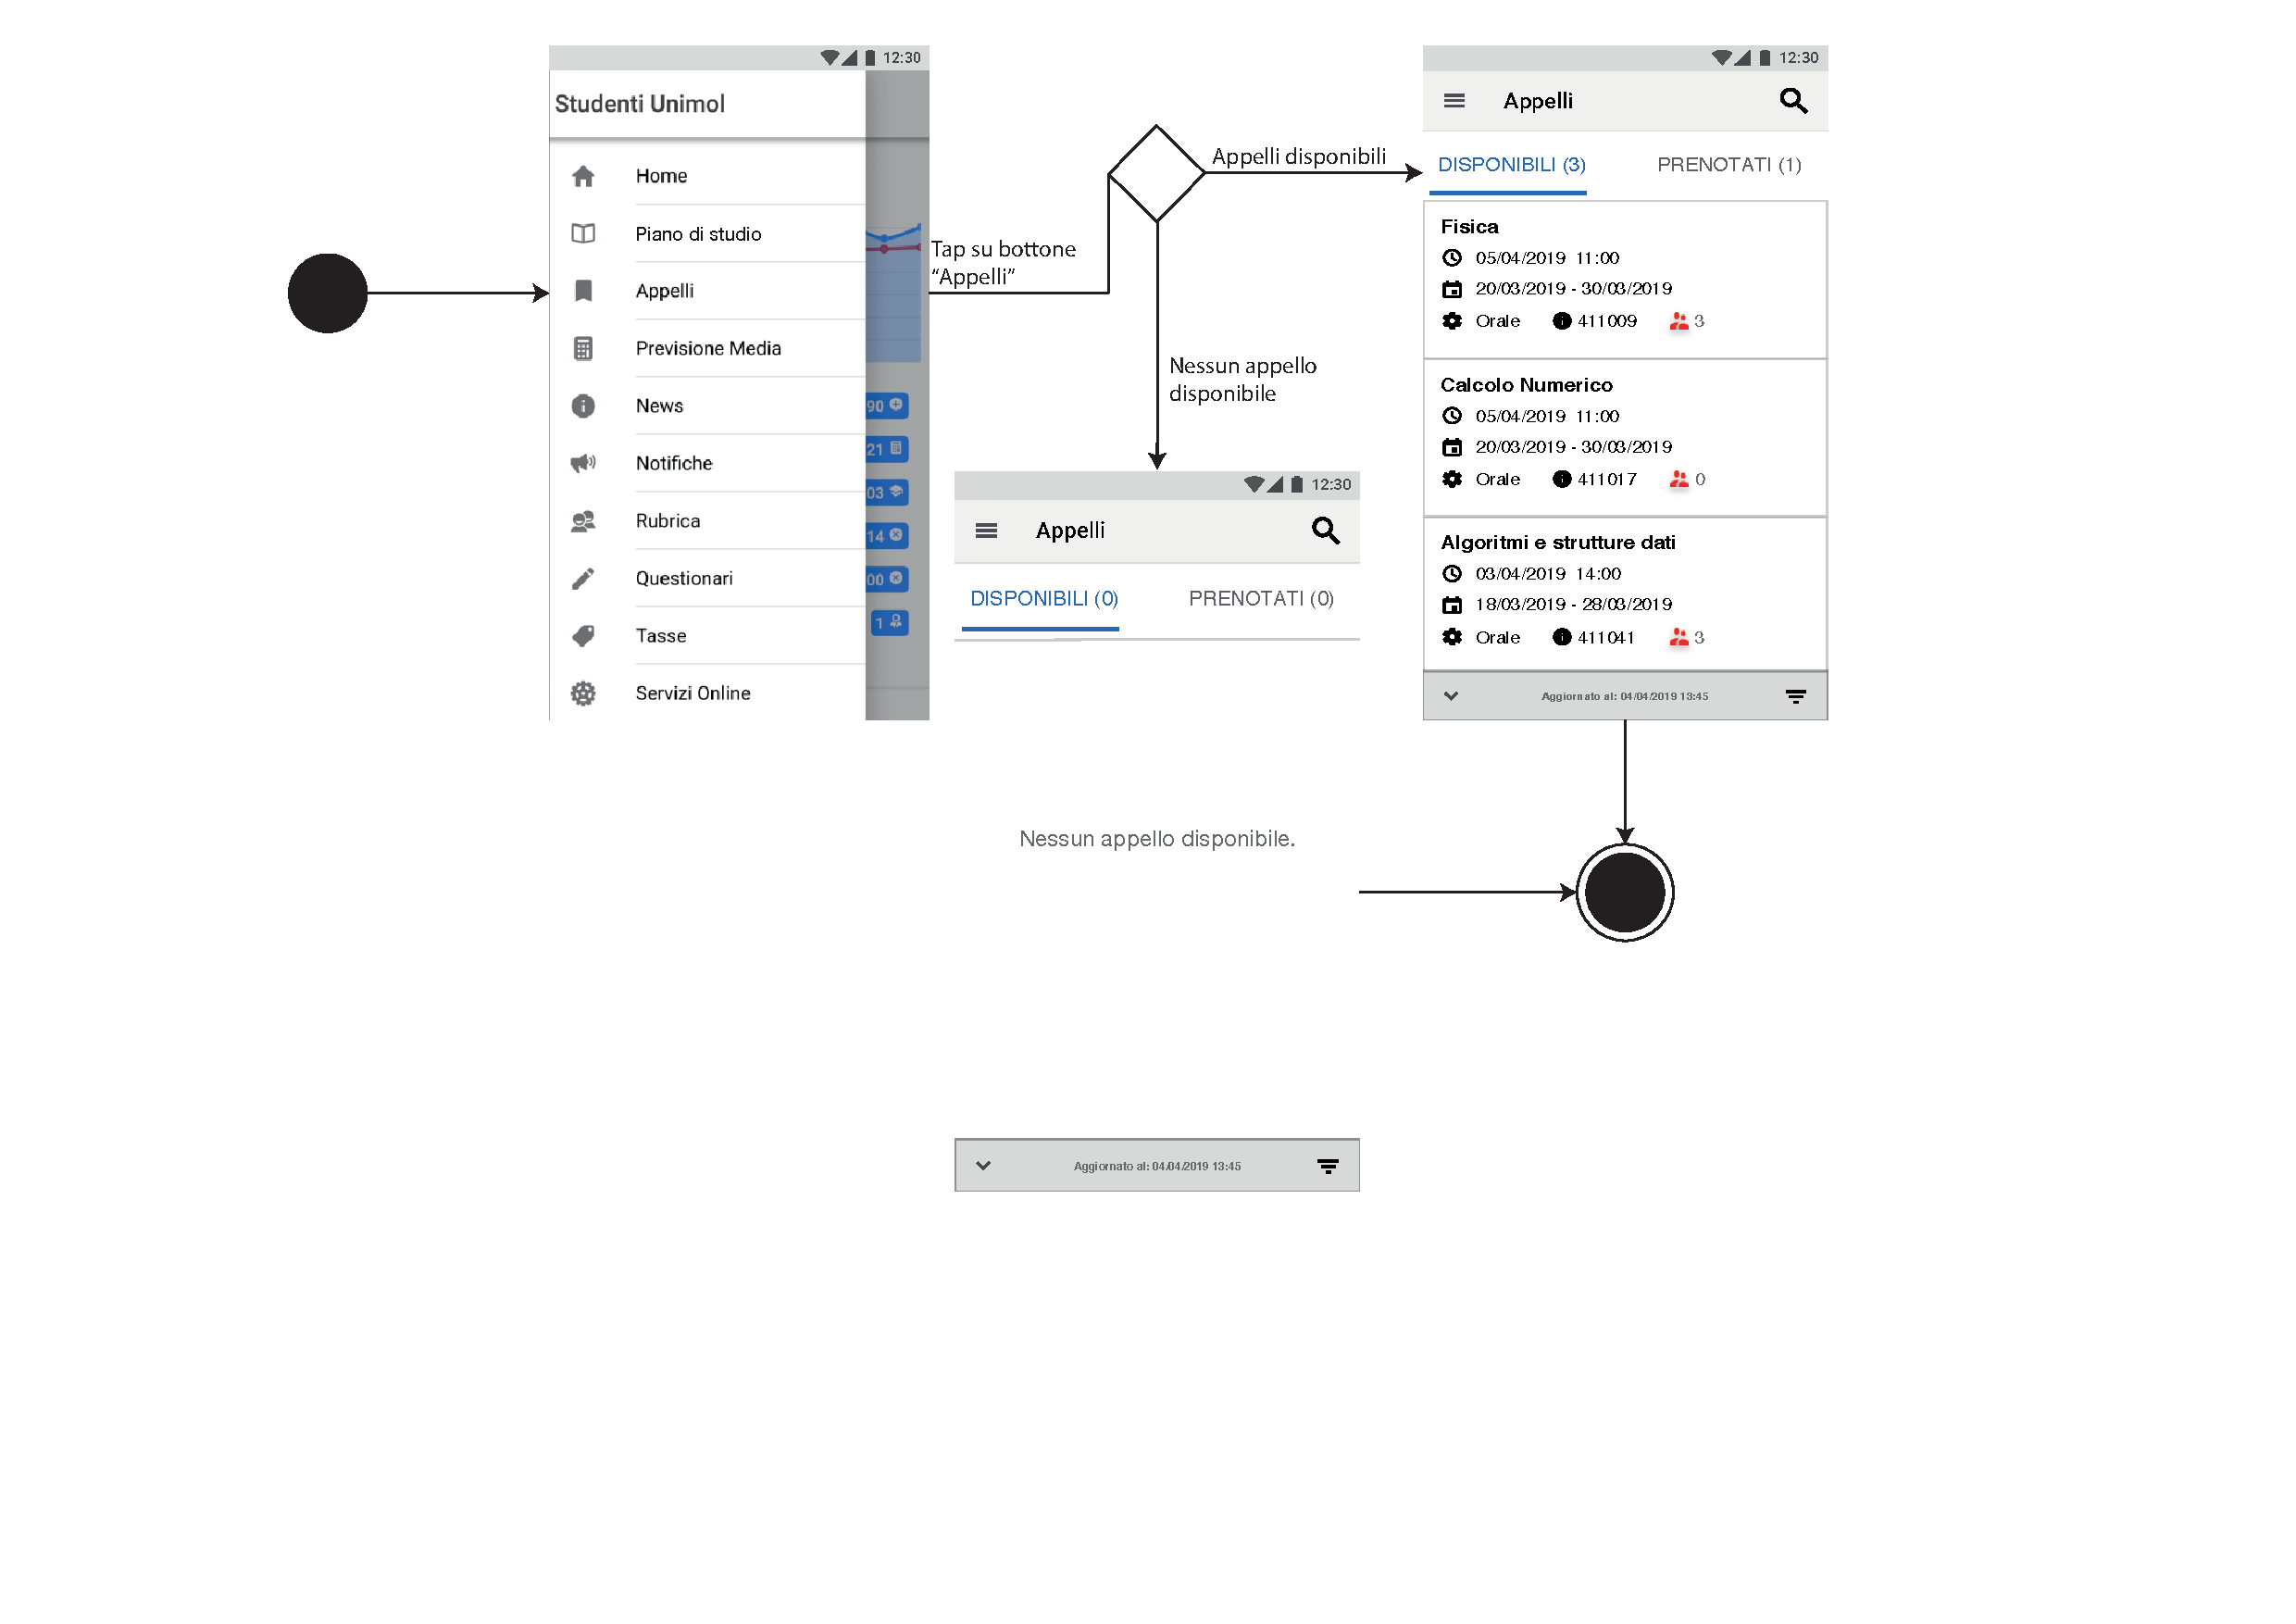
\includegraphics[width=6in]{imgs/gruppo1/activity_diagrams/AD6_visualizza_appelli_disponibili.pdf}
\end{center}
\newpage

%%8.6.7 - Visualizza appelli prenotati%%

\subsection{Visualizza appelli prenotati}
\begin{center}
	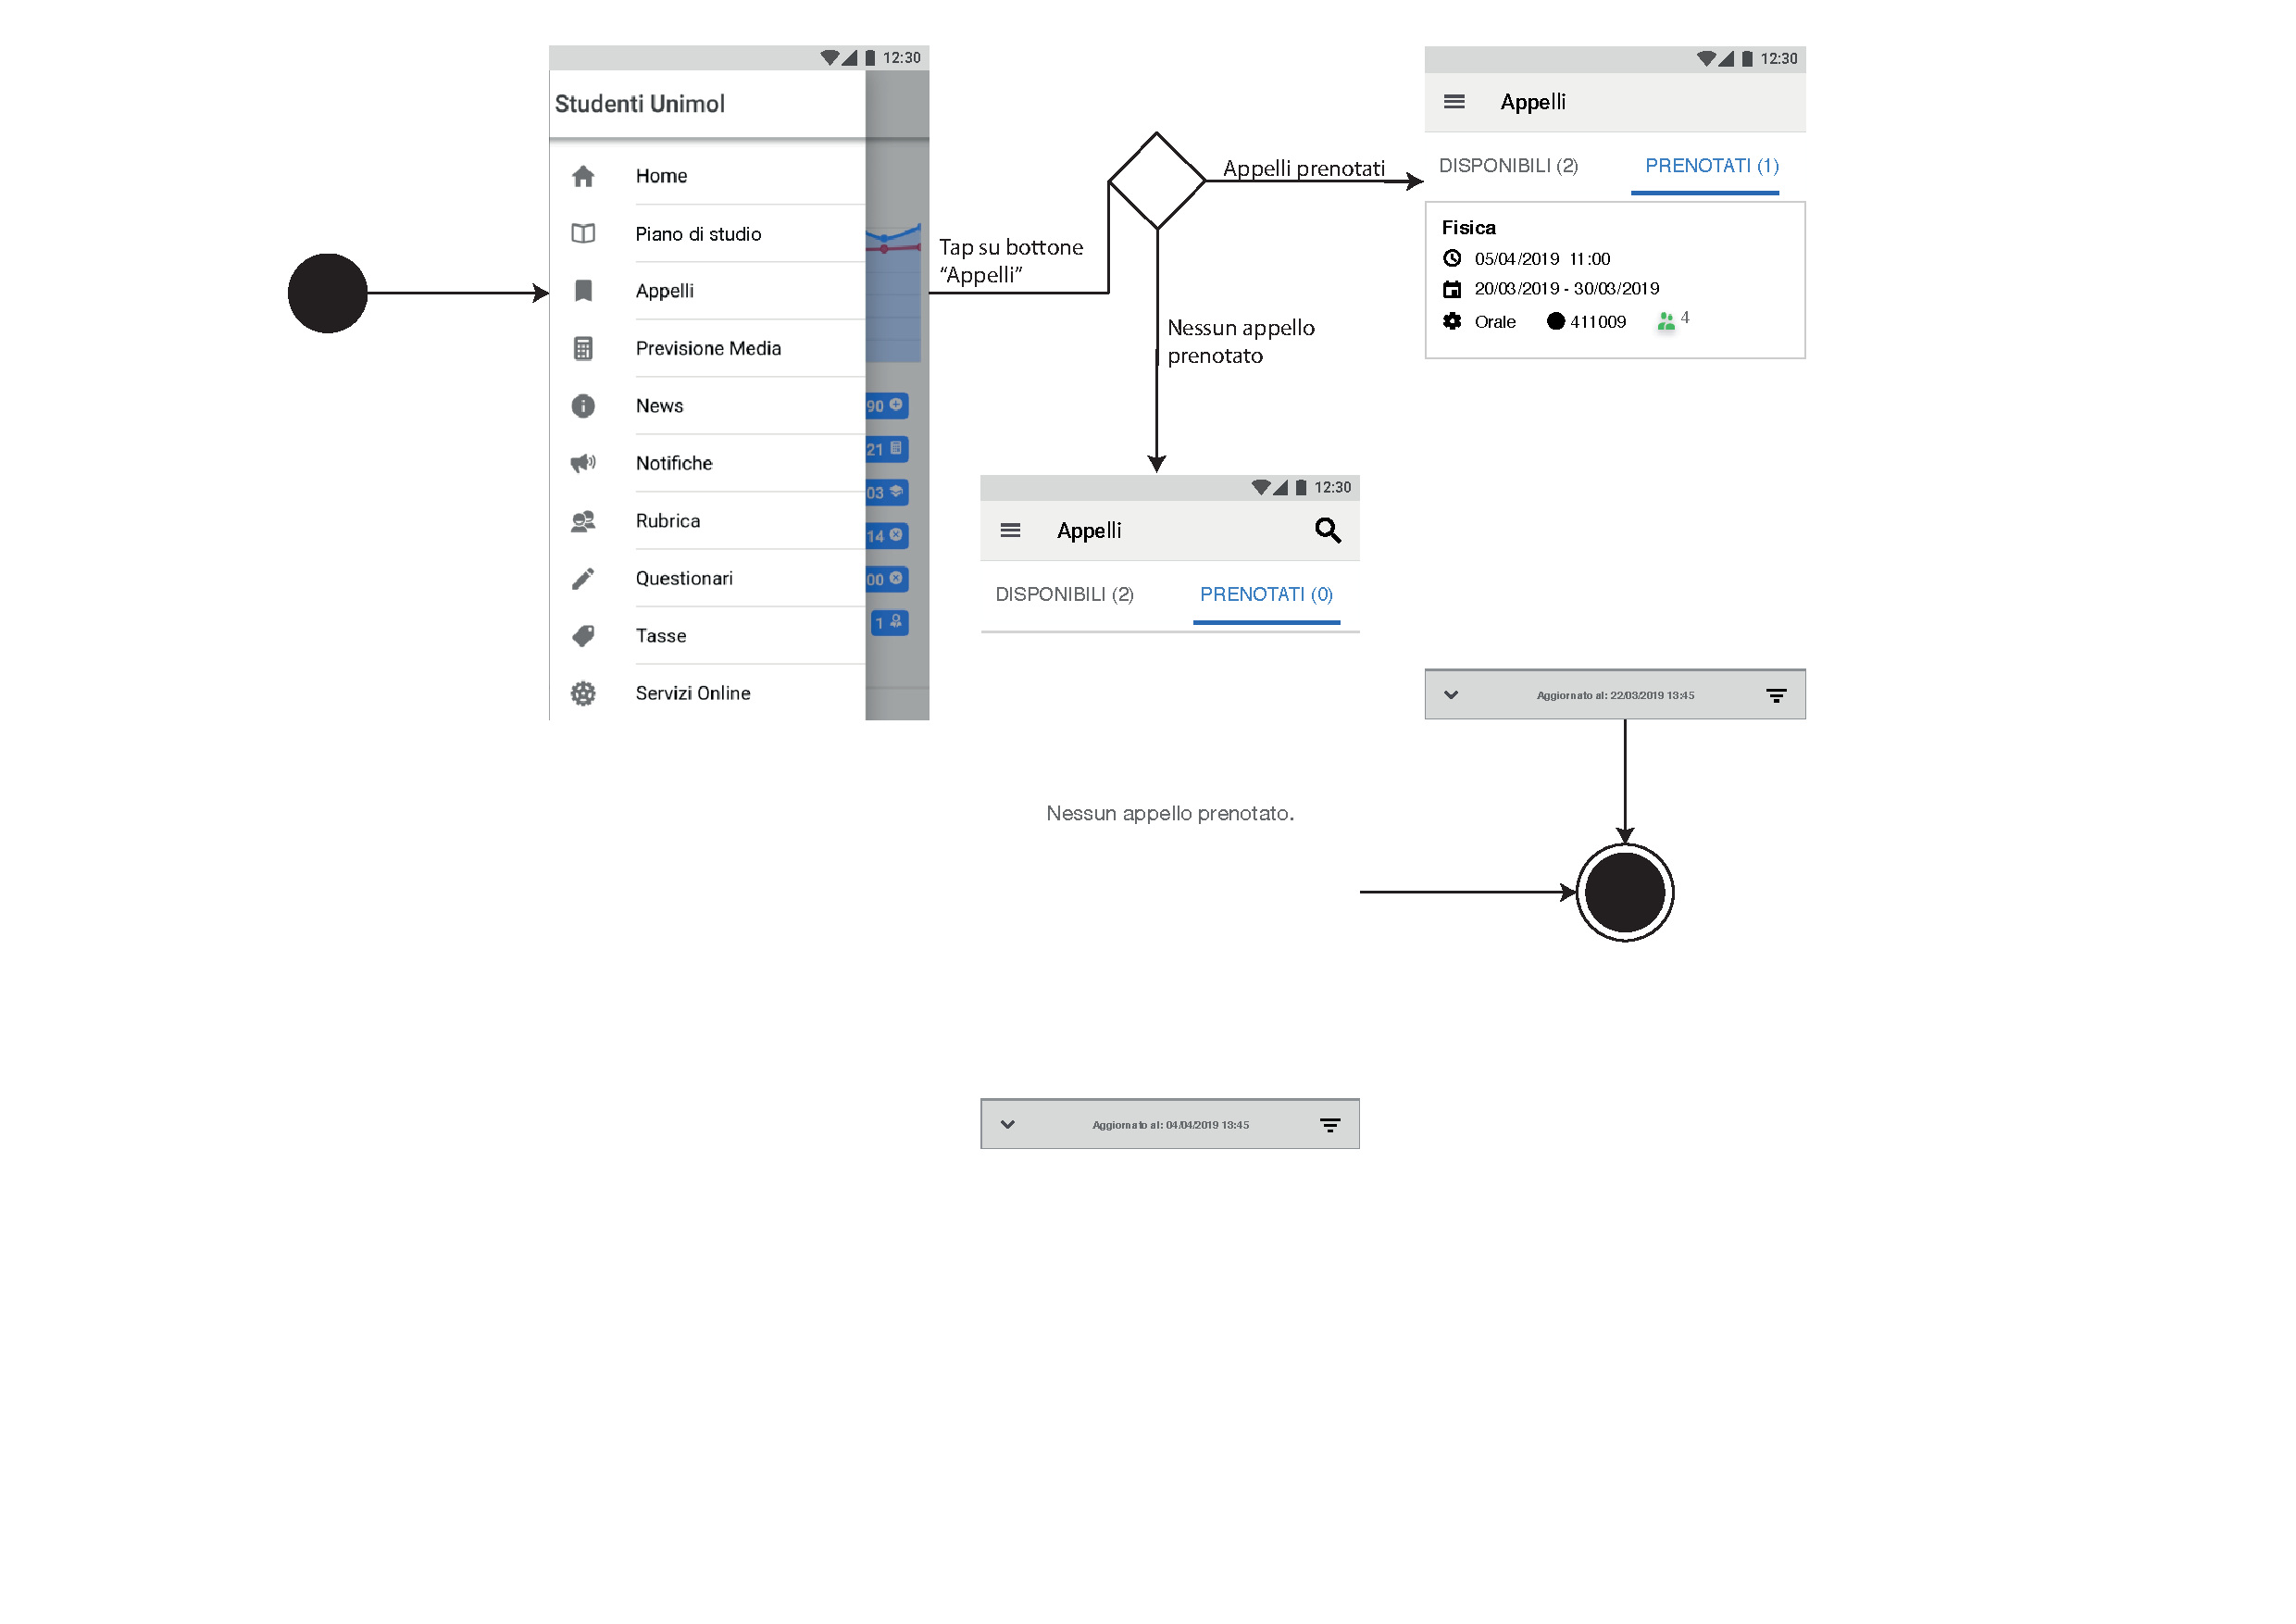
\includegraphics[width=6in]{imgs/gruppo1/activity_diagrams/AD7_visualizza_appelli_prenotati.pdf}
\end{center}
\newpage

%%8.6.8 - Ricerca appelli disponibili %%

\subsection{Ricerca appelli disponibili}
\begin{center}
	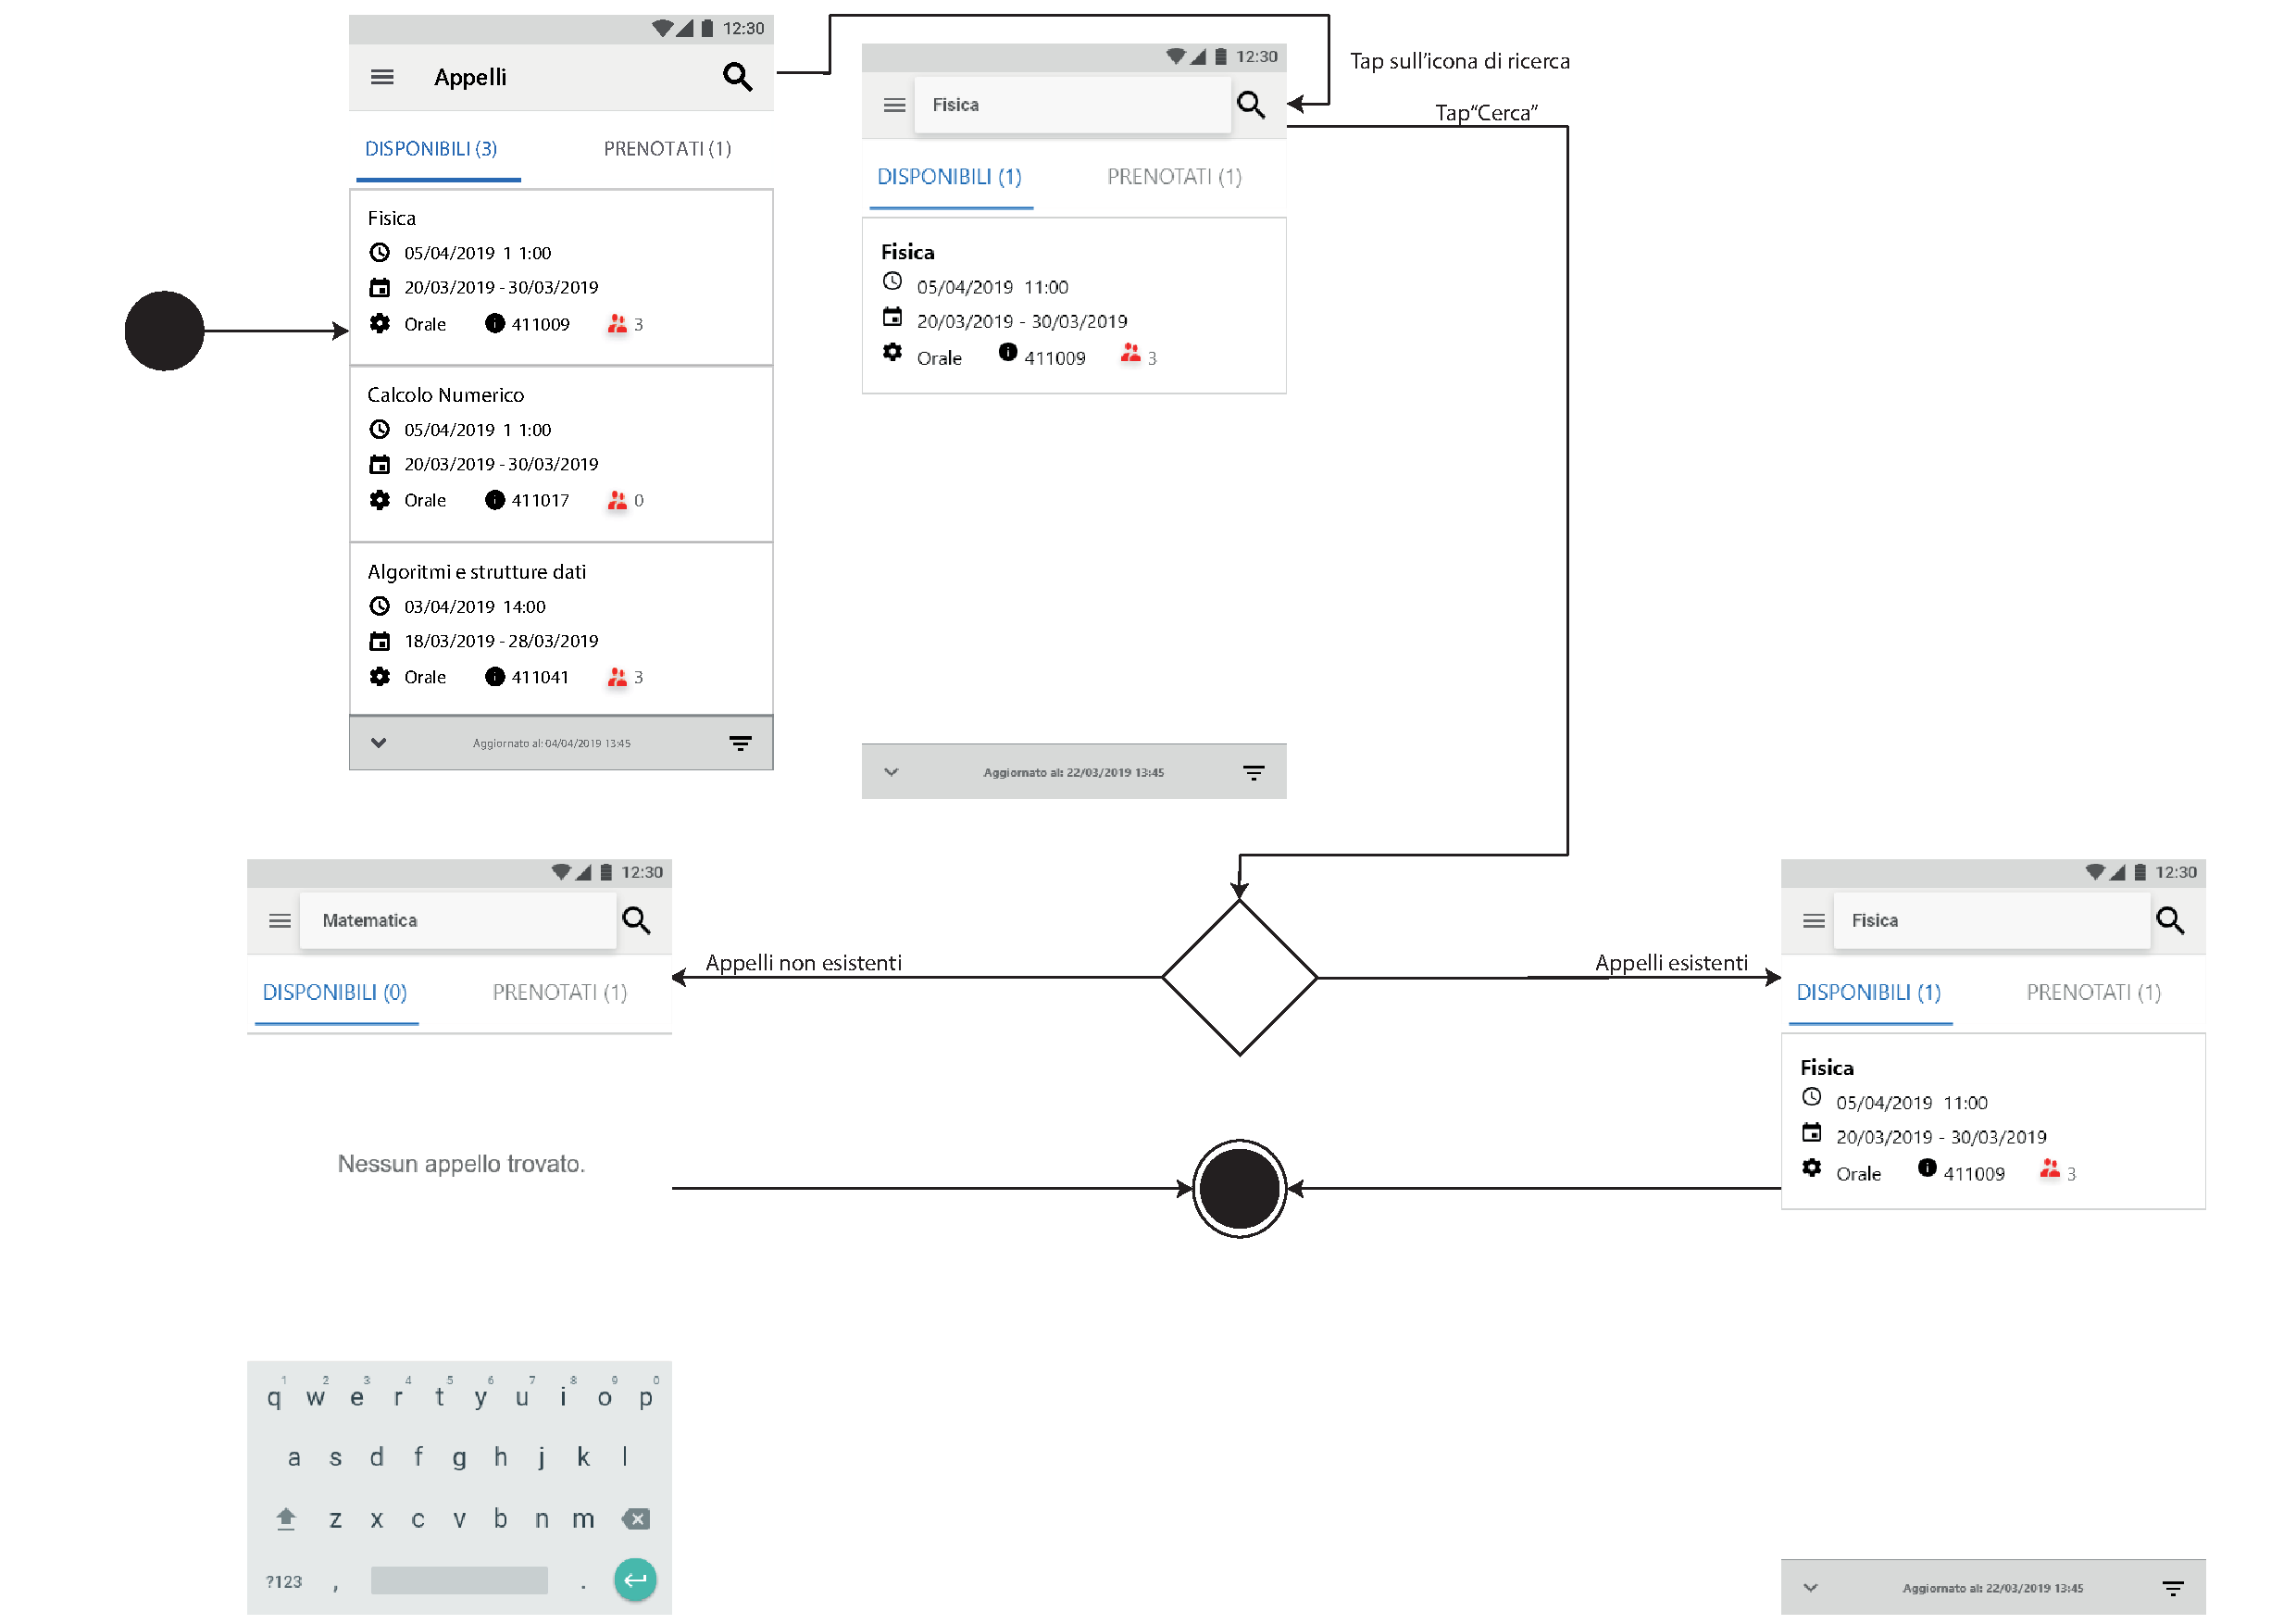
\includegraphics[width=6in]{imgs/gruppo1/activity_diagrams/AD8_Ricerca_appelli.pdf}
\end{center}
\newpage

%%8.6.9 - Filtra appelli disponibili con memorizzazione %%

\subsection{Filtra appelli disponibili con memorizzazione }
\begin{center}
	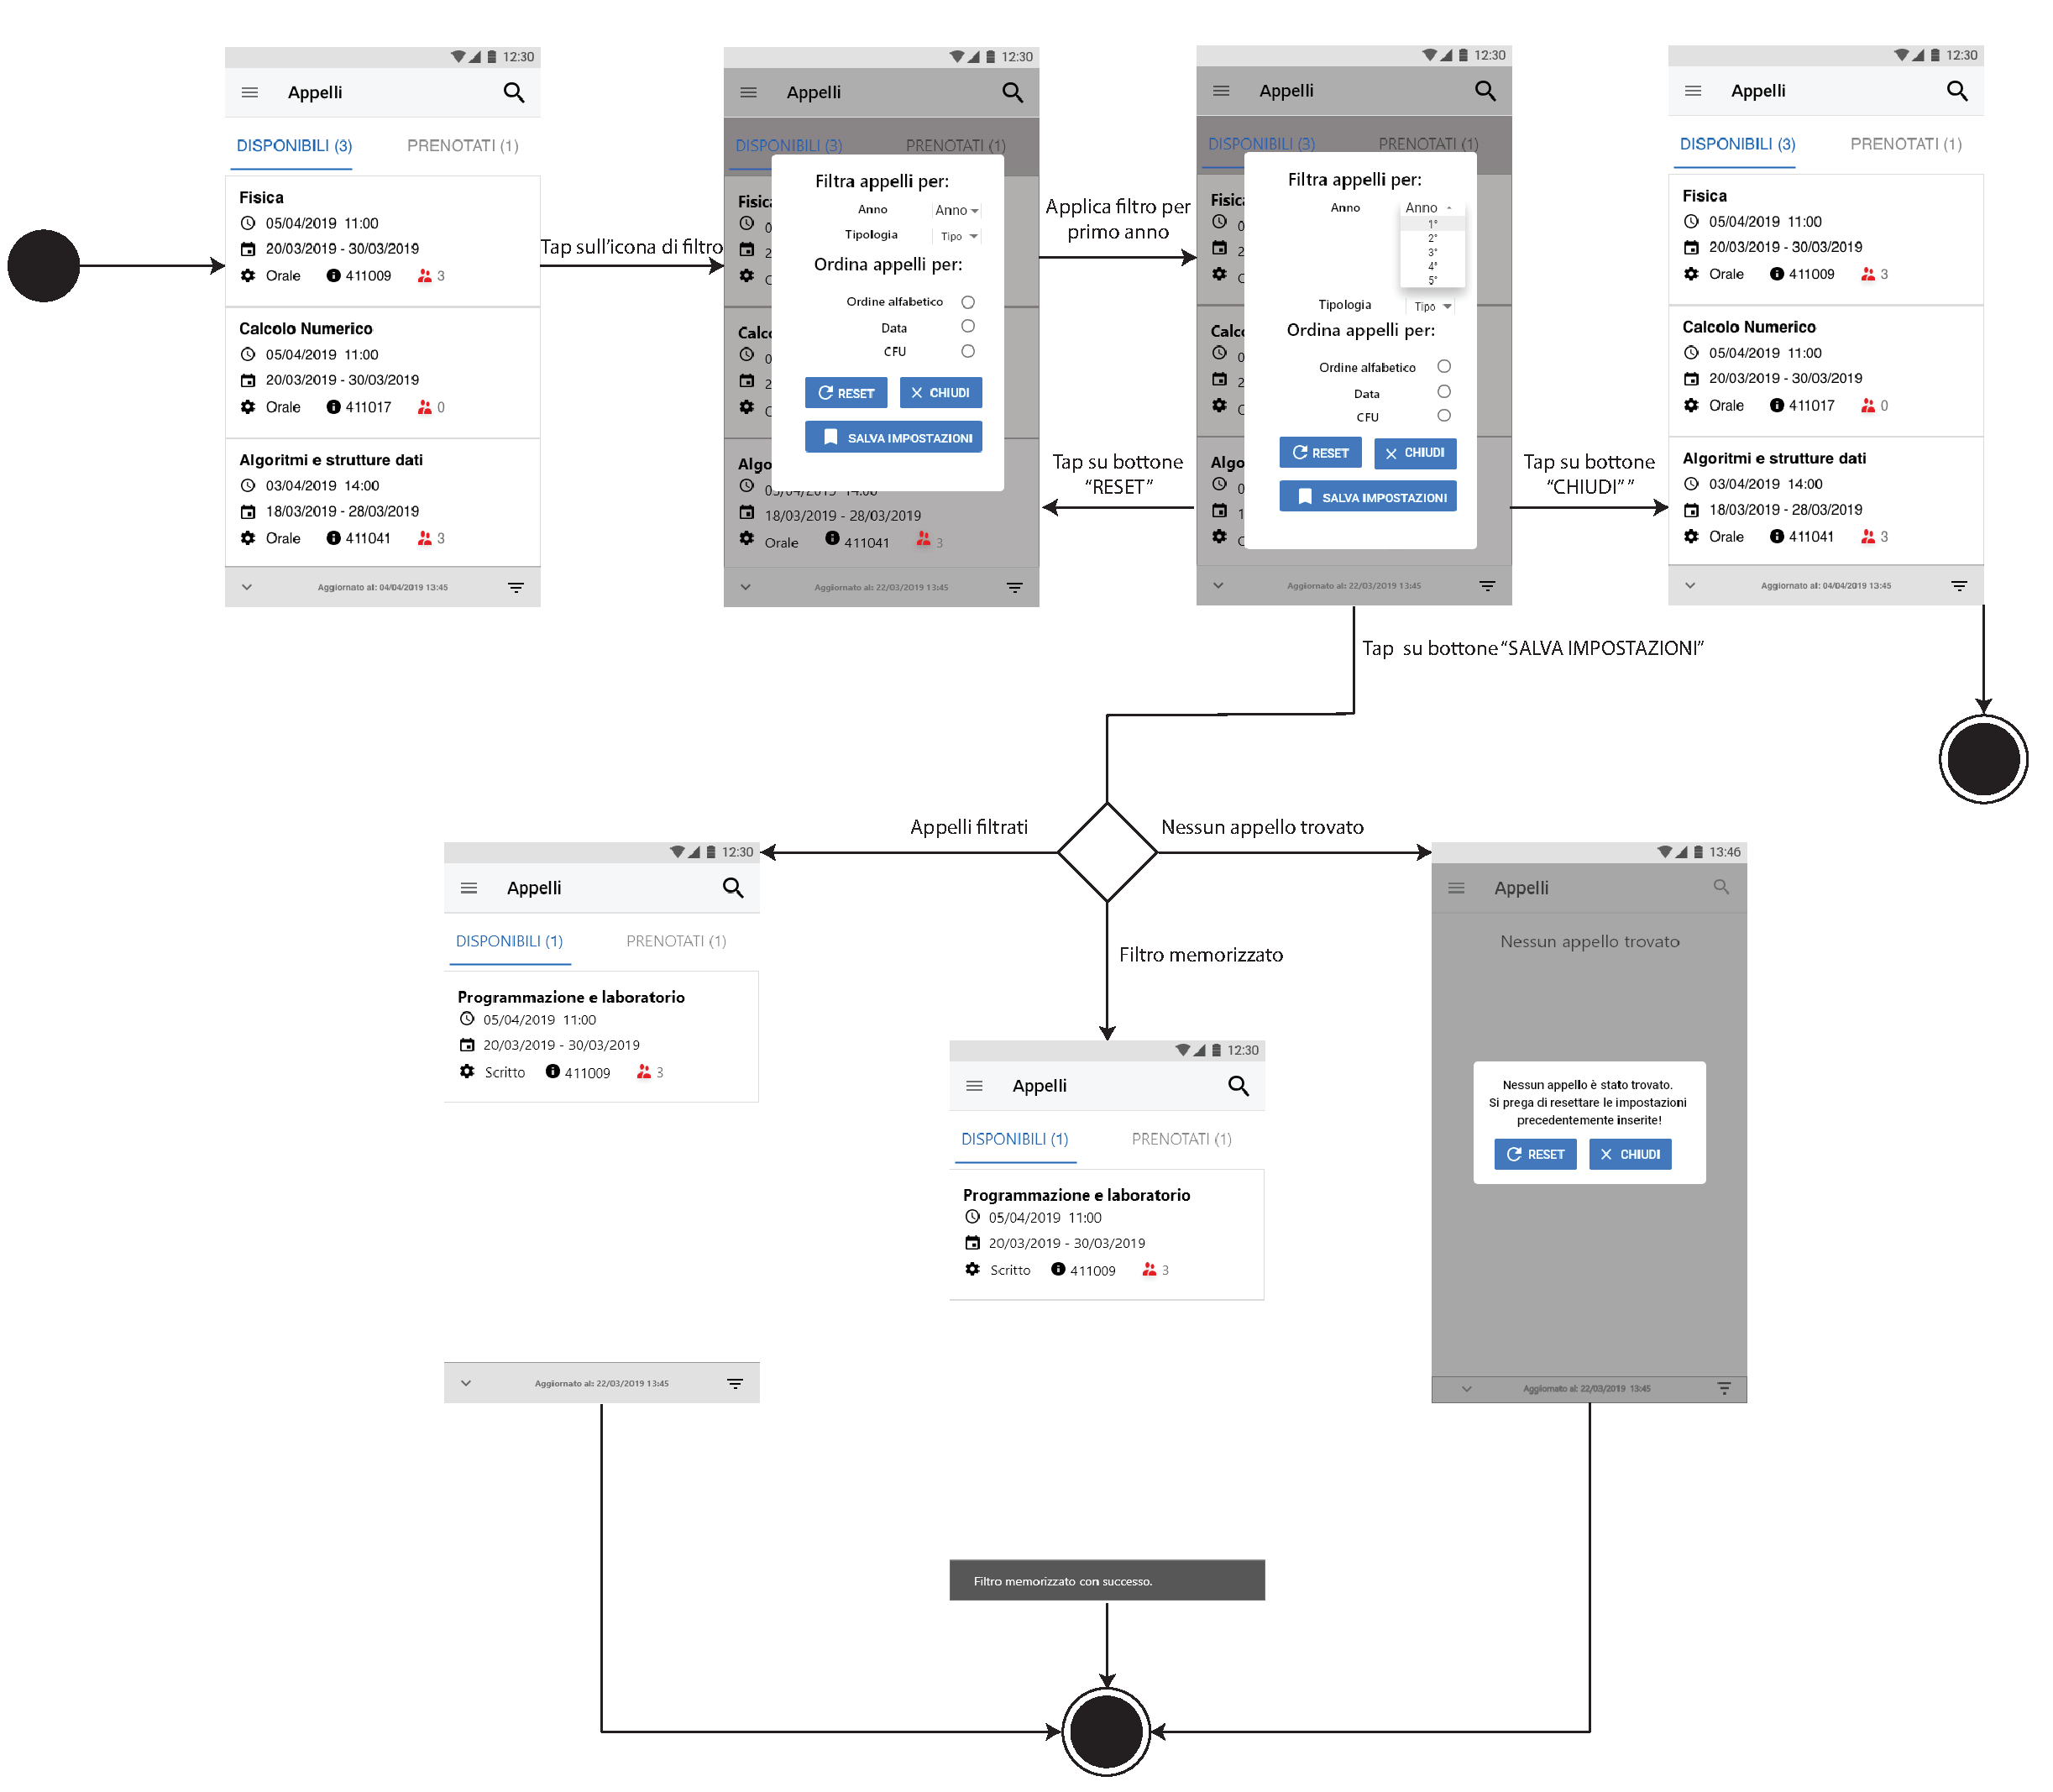
\includegraphics[width=6in]{imgs/gruppo1/activity_diagrams/AD9_filtrati_appelli.pdf}
\end{center}
\newpage

%%8.6.10 - Ordina appelli disponibili con memorizzazione%%

\subsection{Ordina appelli disponibili con memorizzazione }
\begin{center}
	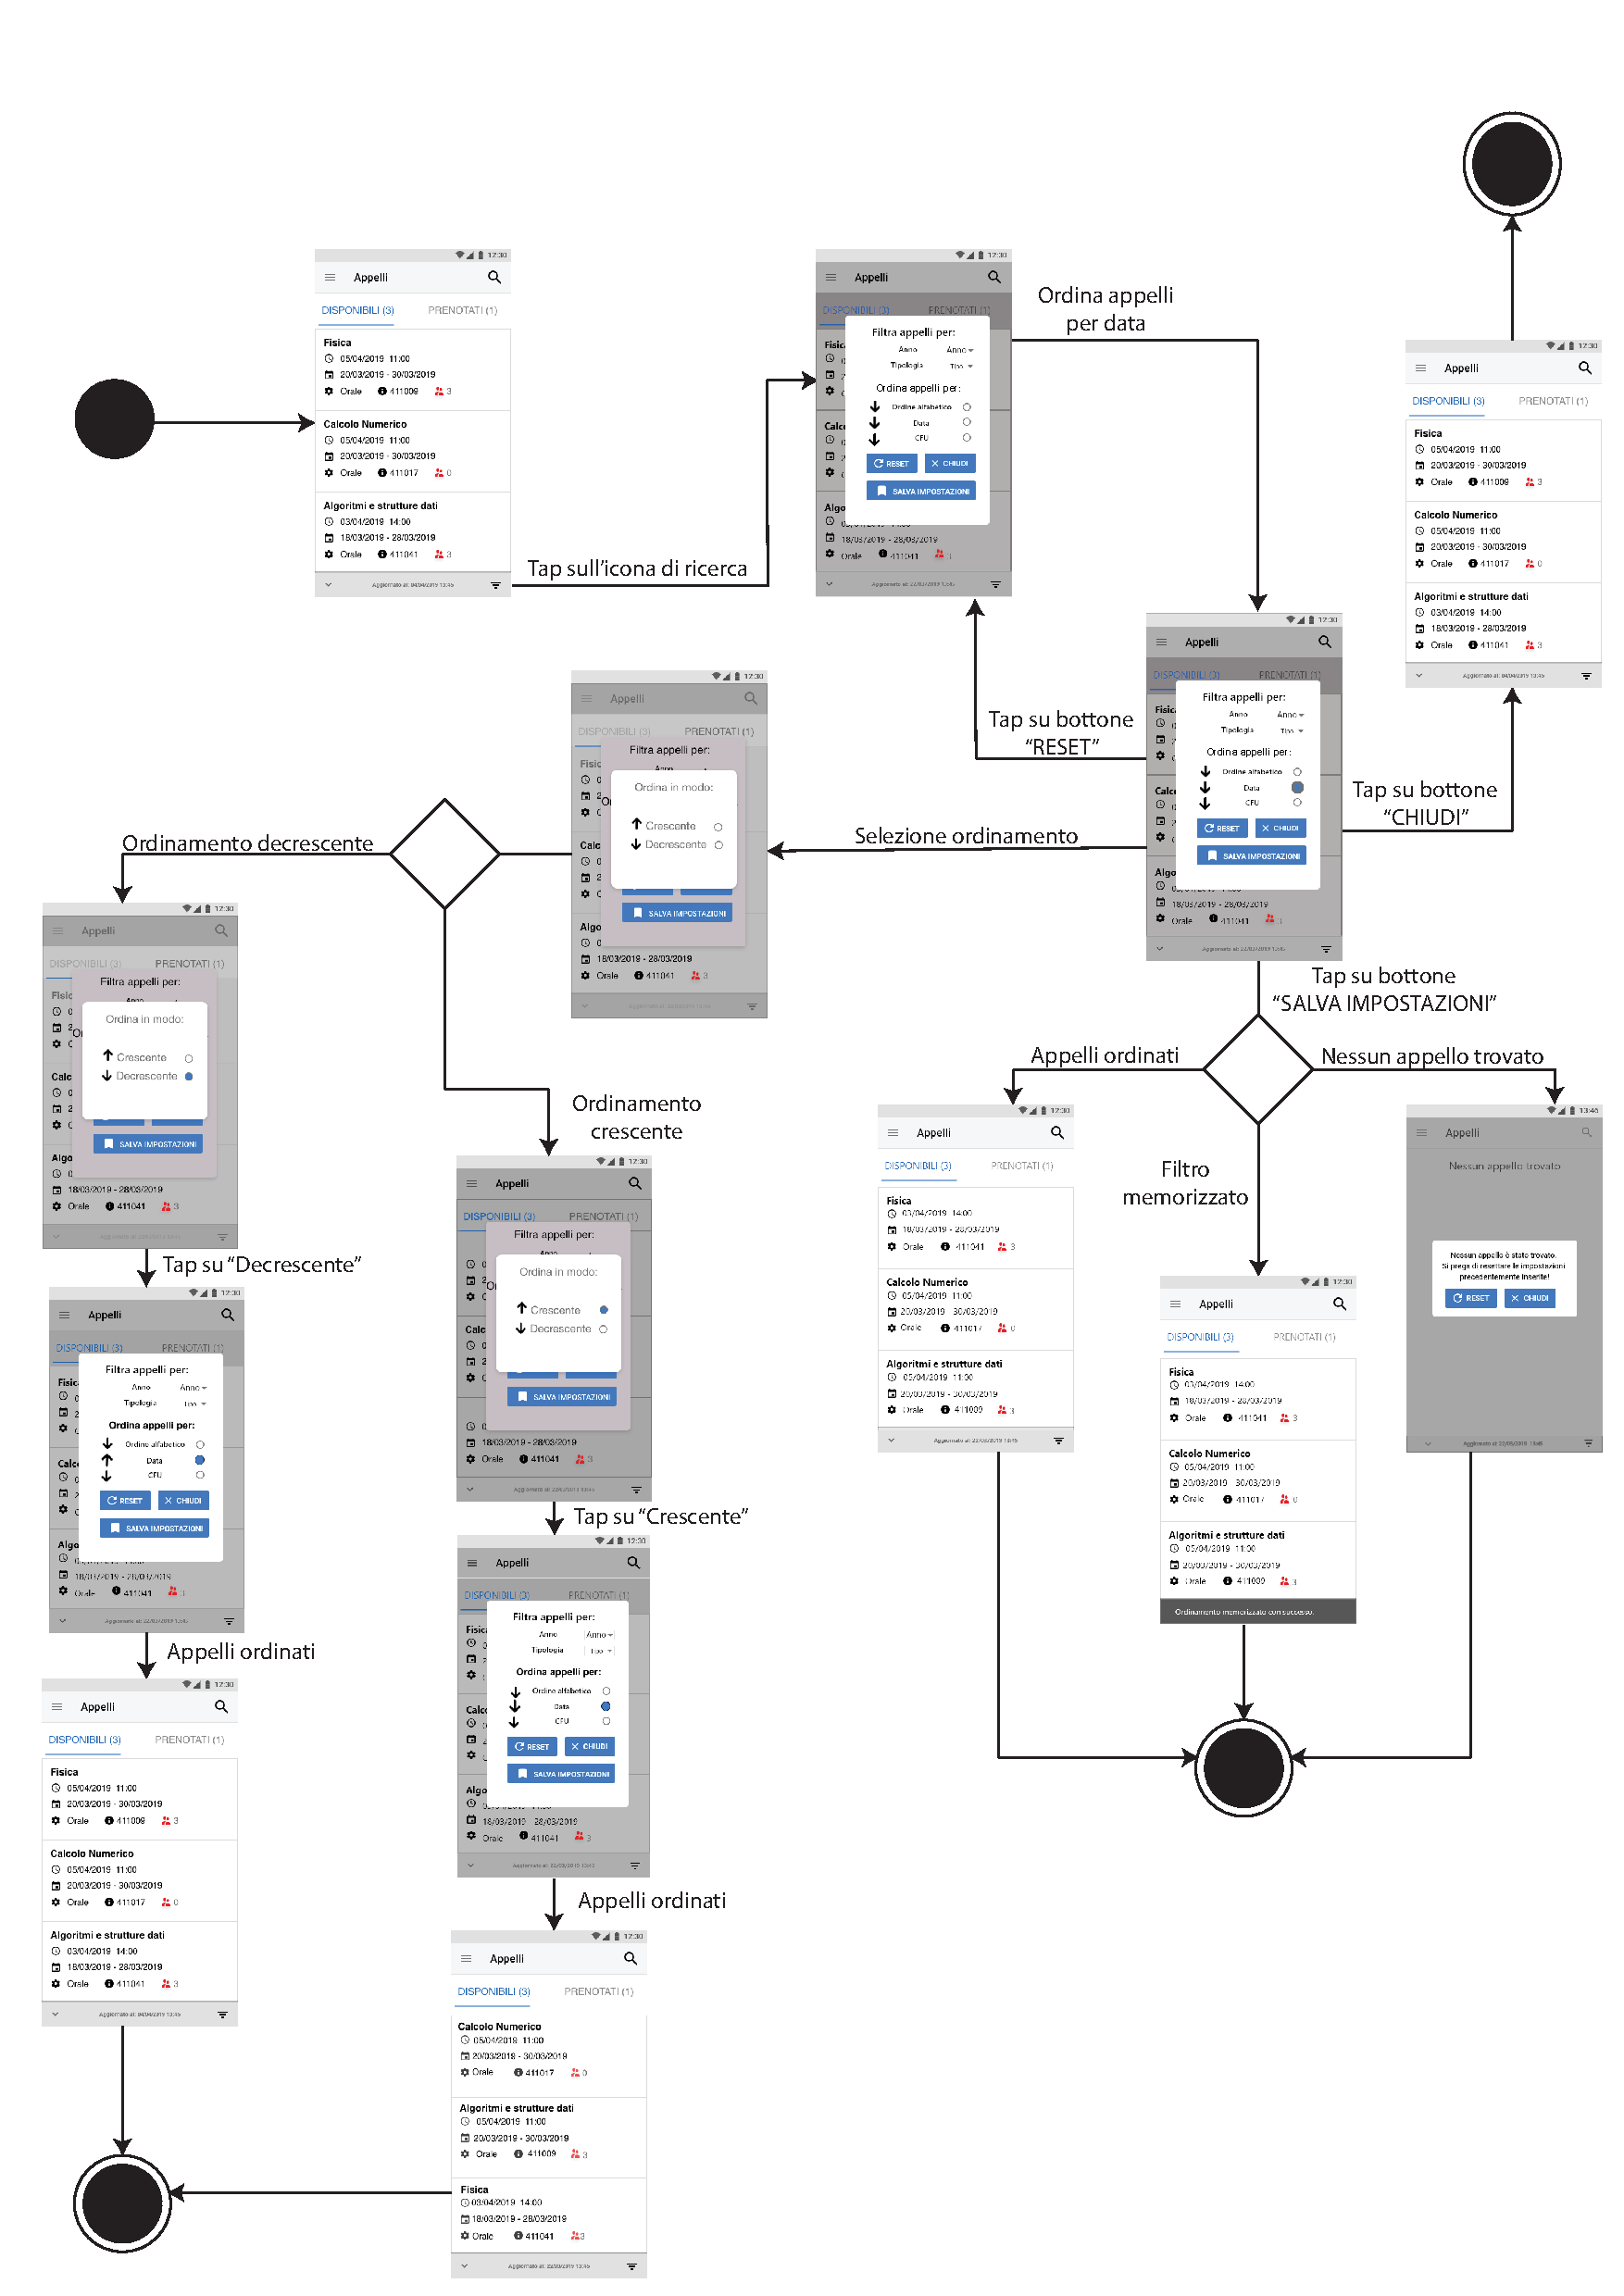
\includegraphics[width=6in]{imgs/gruppo1/activity_diagrams/AD10_ordina_appelli.pdf}
\end{center}
\newpage

%%8.6.11 - Prenota appello%%

\subsection{Prenota appello }
\begin{center}
	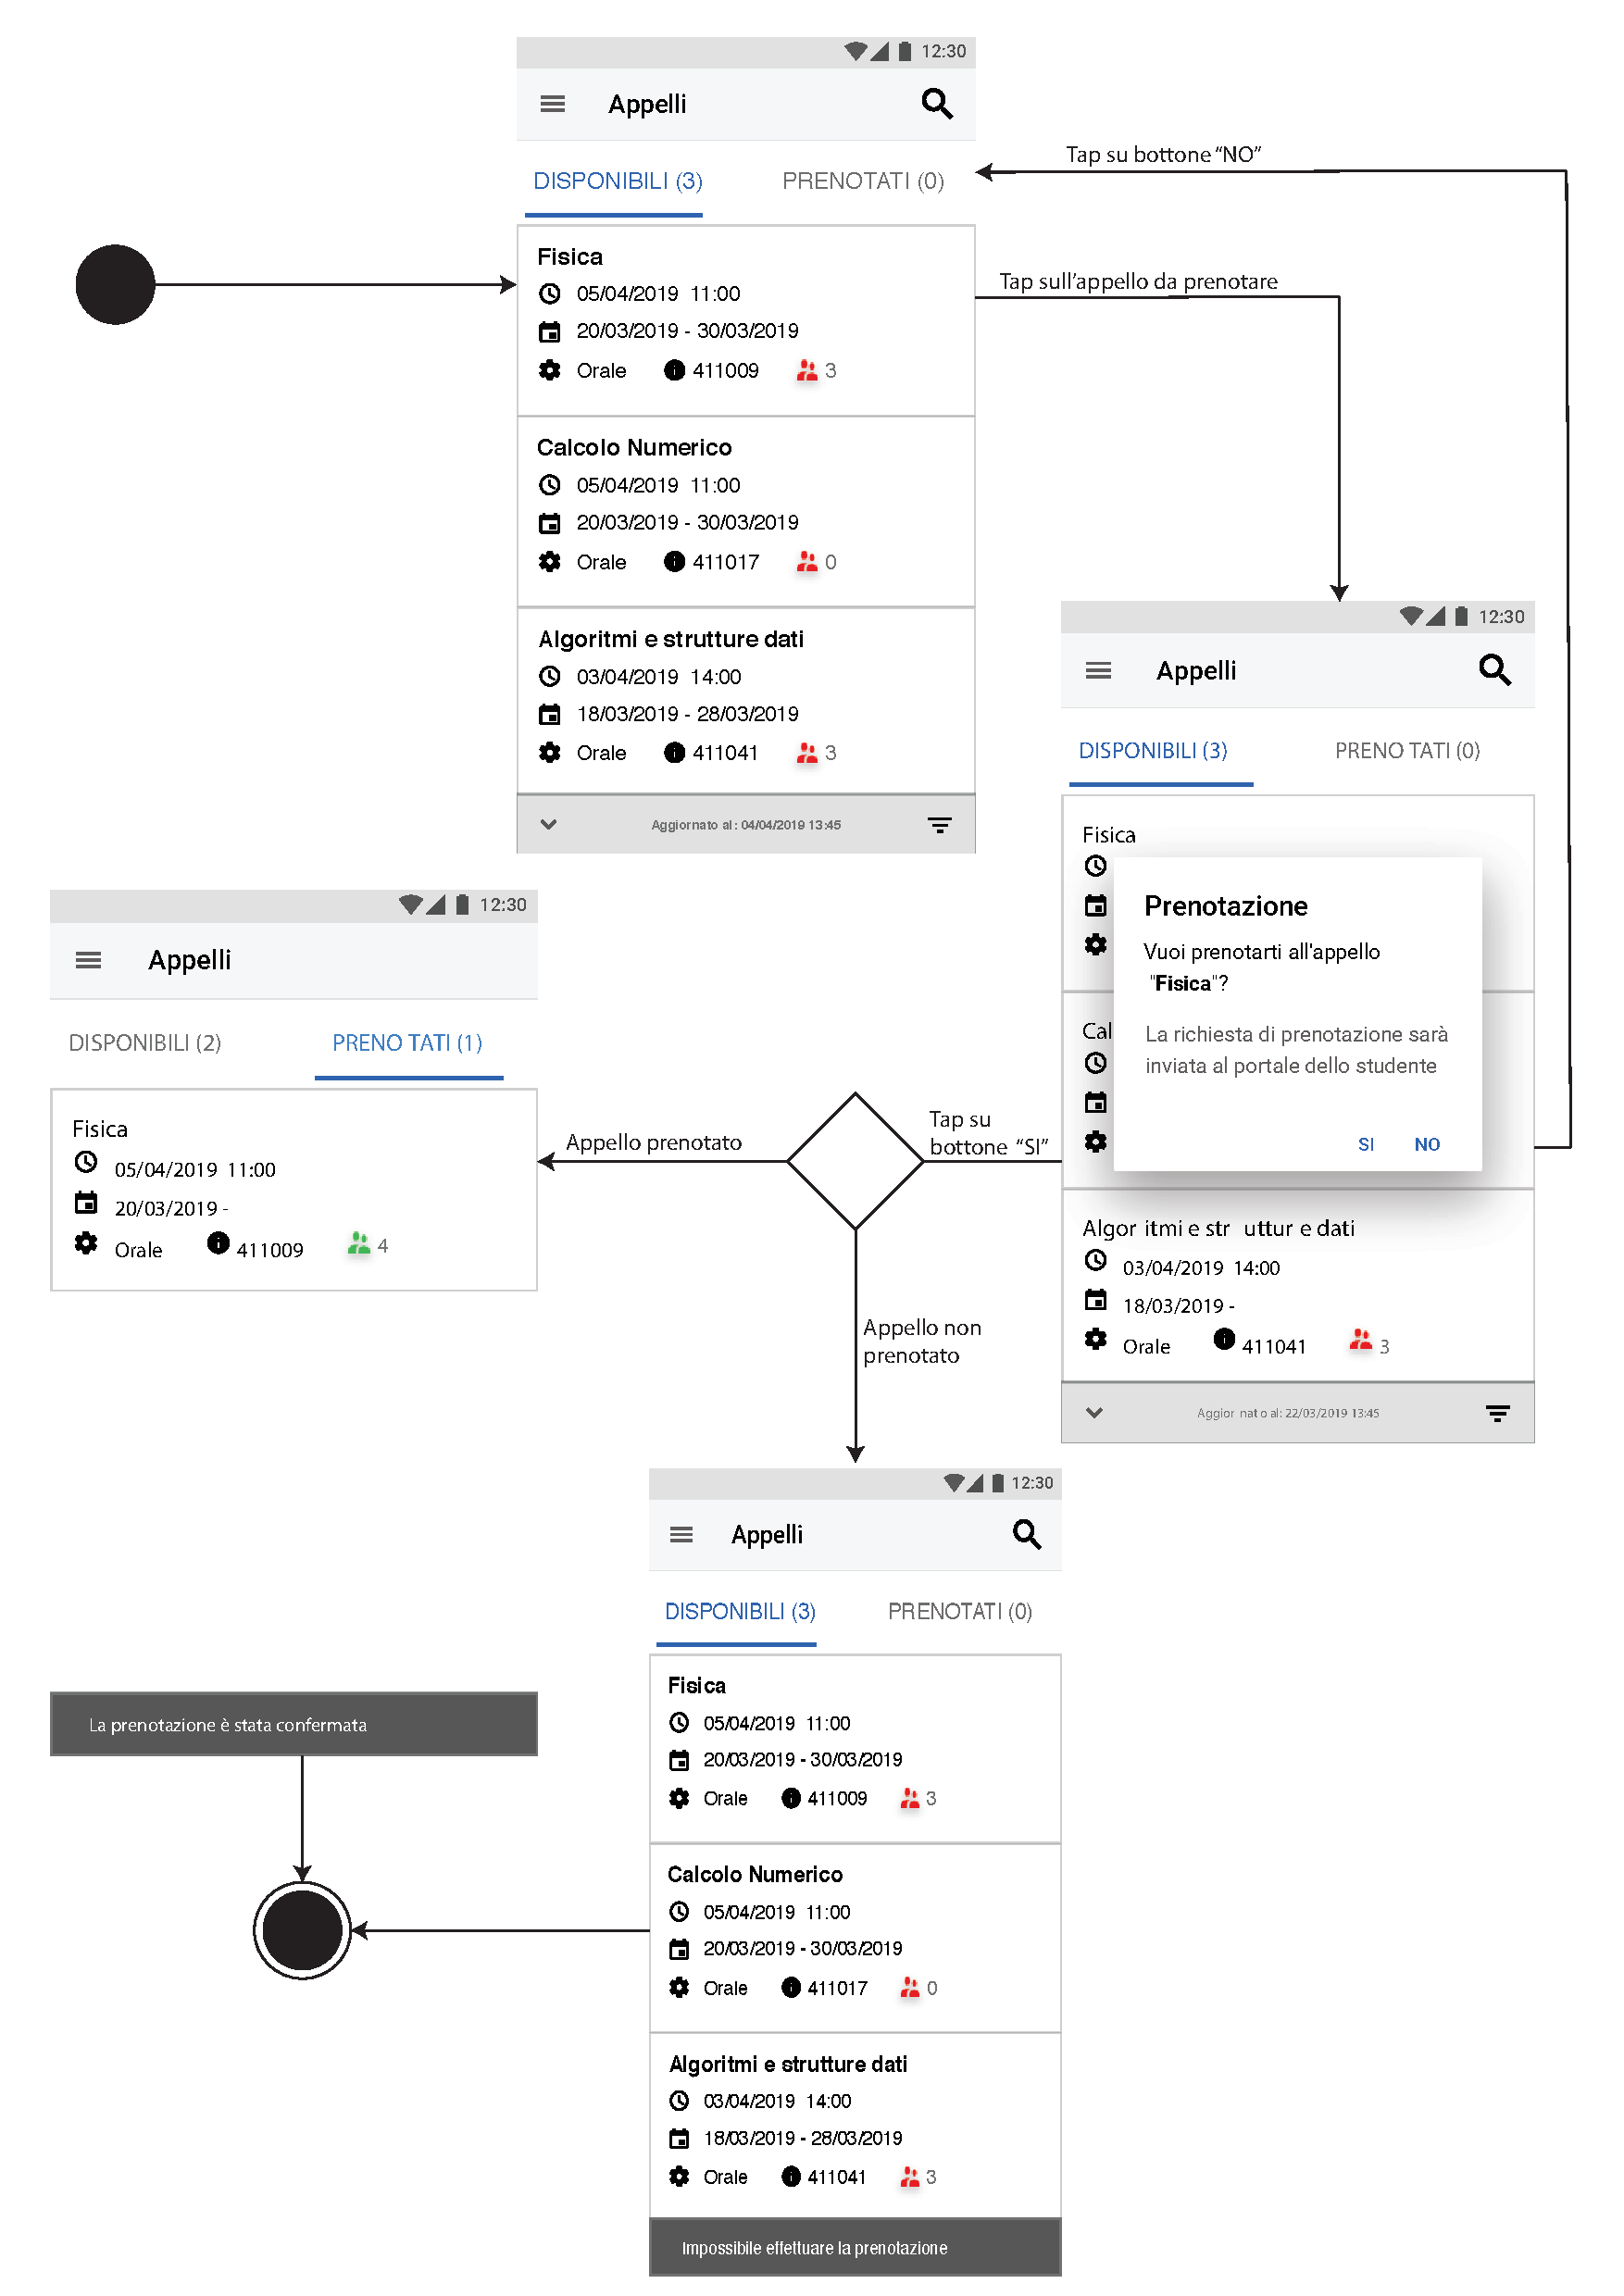
\includegraphics[width=6in]{imgs/gruppo1/activity_diagrams/AD11_prenota_apppello.pdf}
\end{center}
\newpage

%%8.6.12 - Cancella prenotazione%%

\subsection{Cancella prenotazione}
\begin{center}
	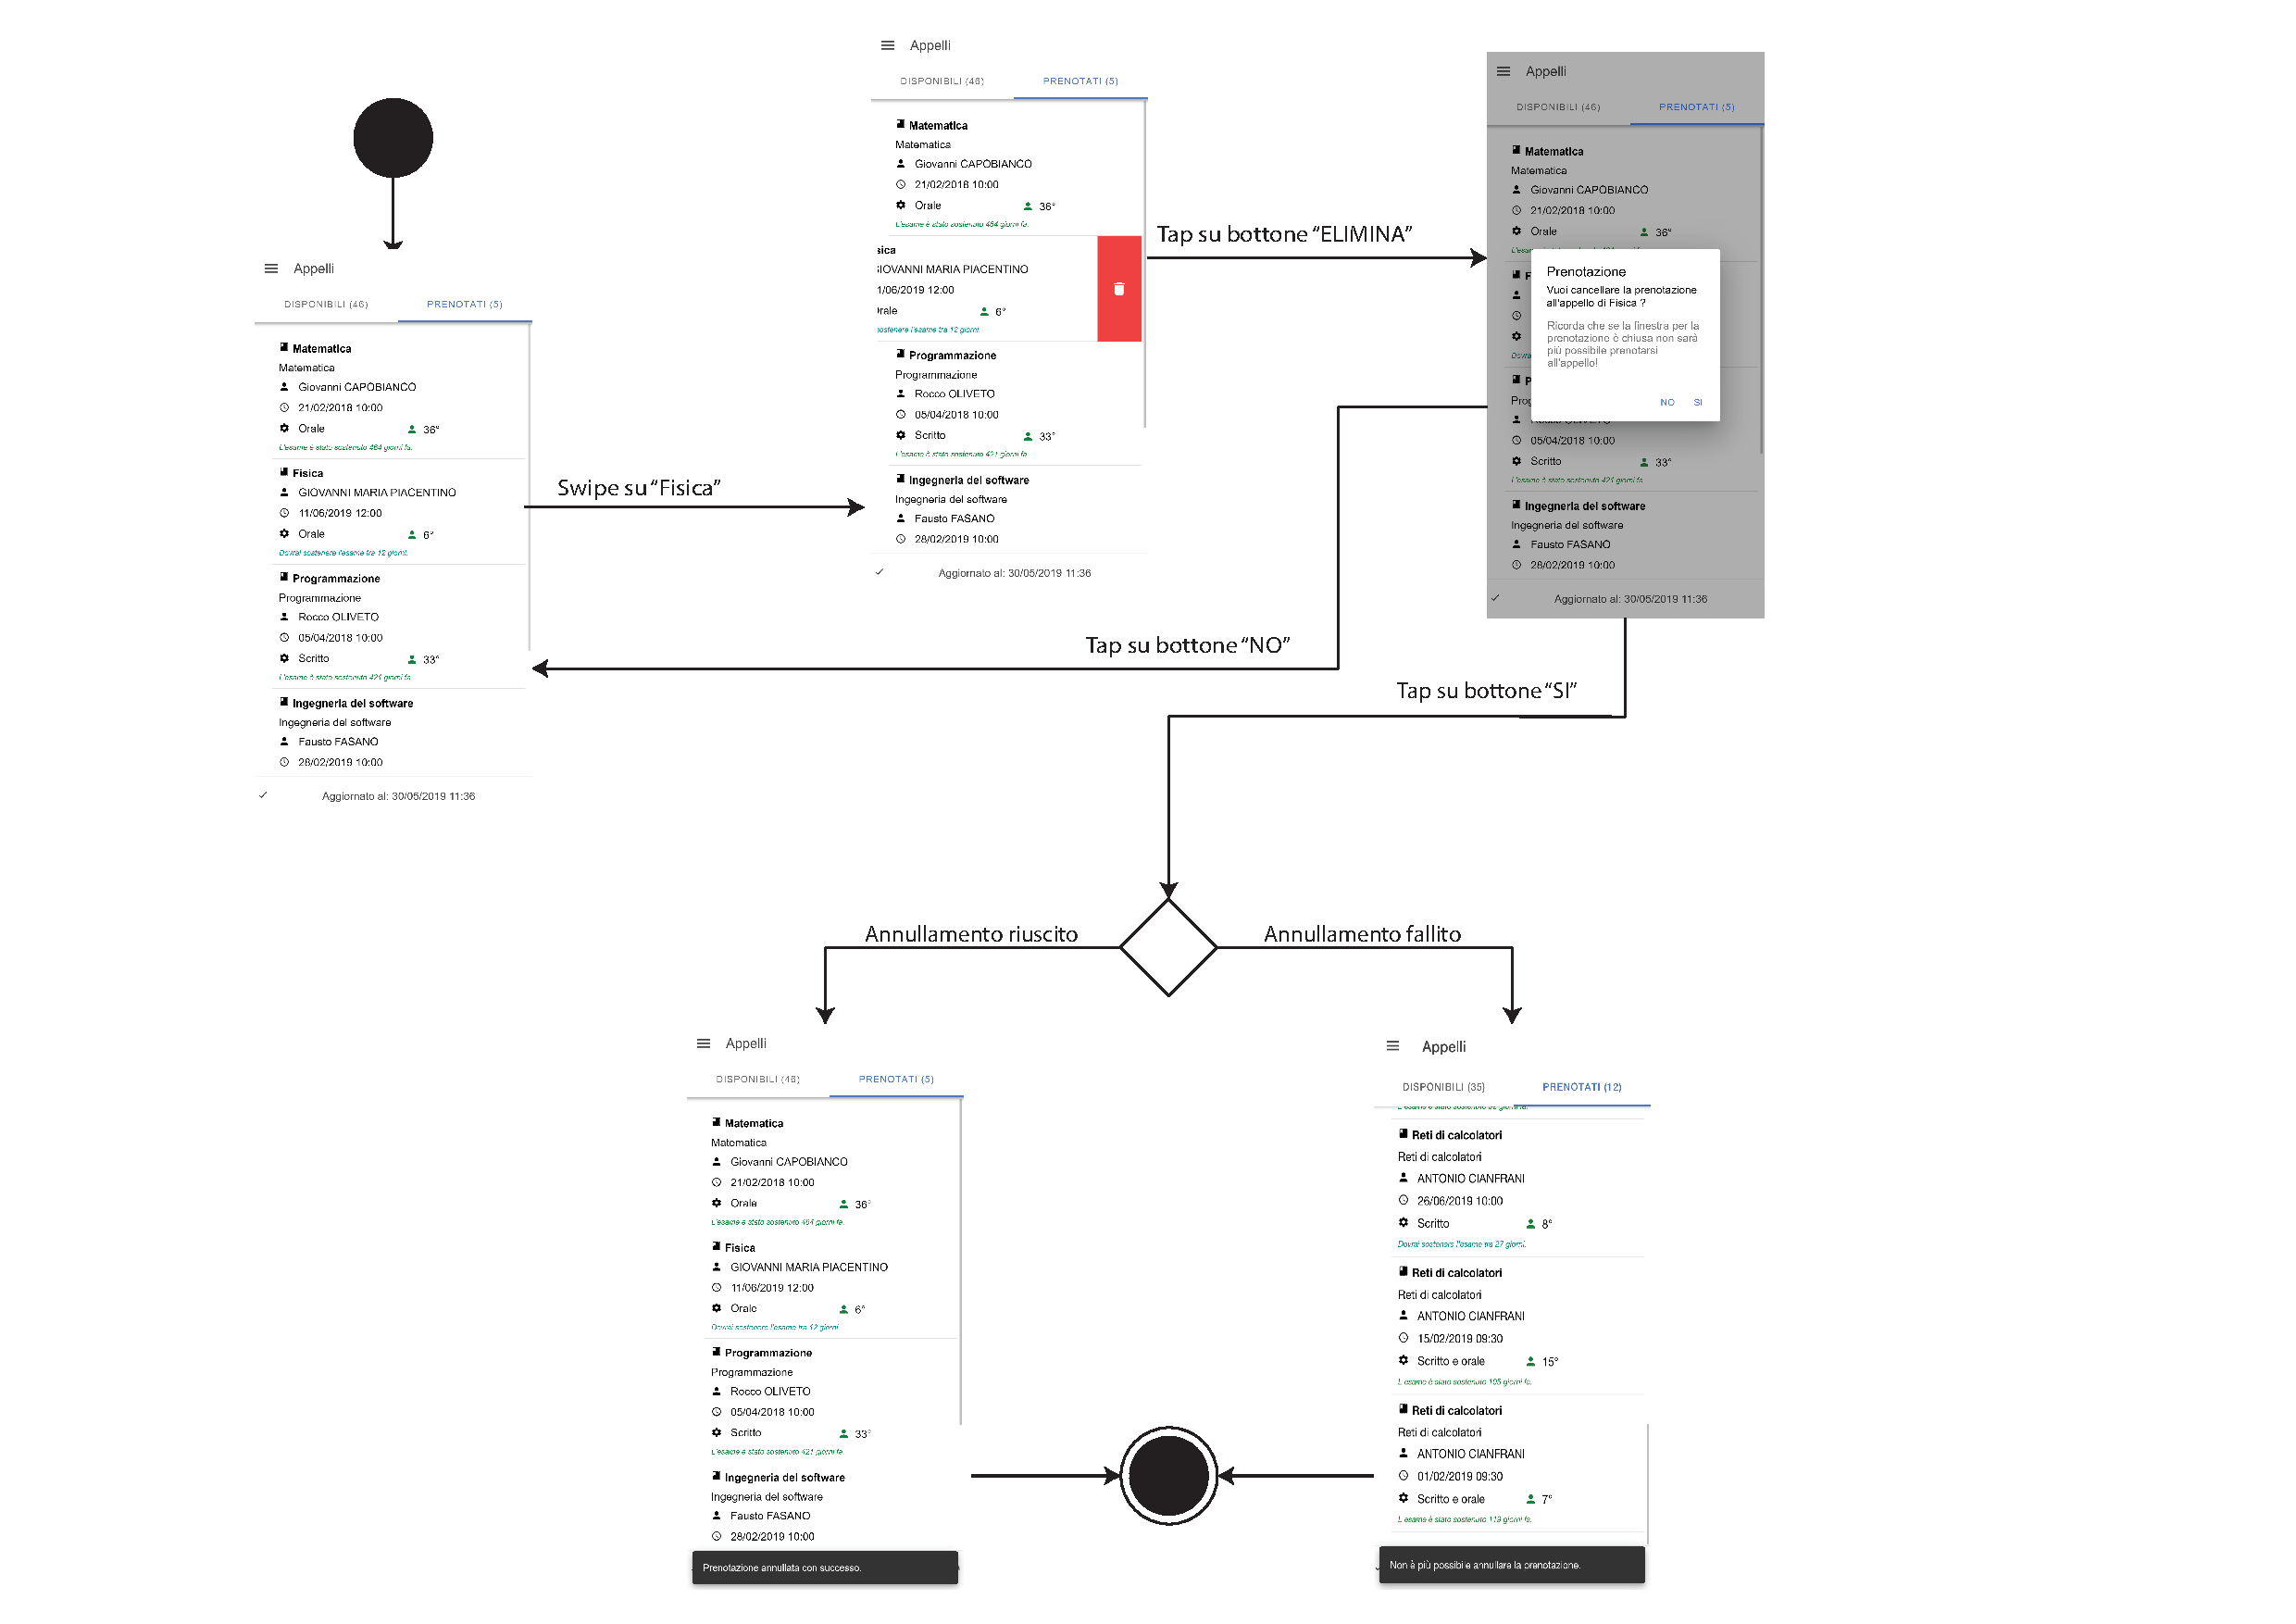
\includegraphics[width=6in]{imgs/gruppo1/activity_diagrams/AD12_cancella_prenotazione.pdf}
\end{center}
\newpage

%%8.6.13 - Visualizza elenco file%%

\subsection{Visualizza elenco file}
\begin{center}
	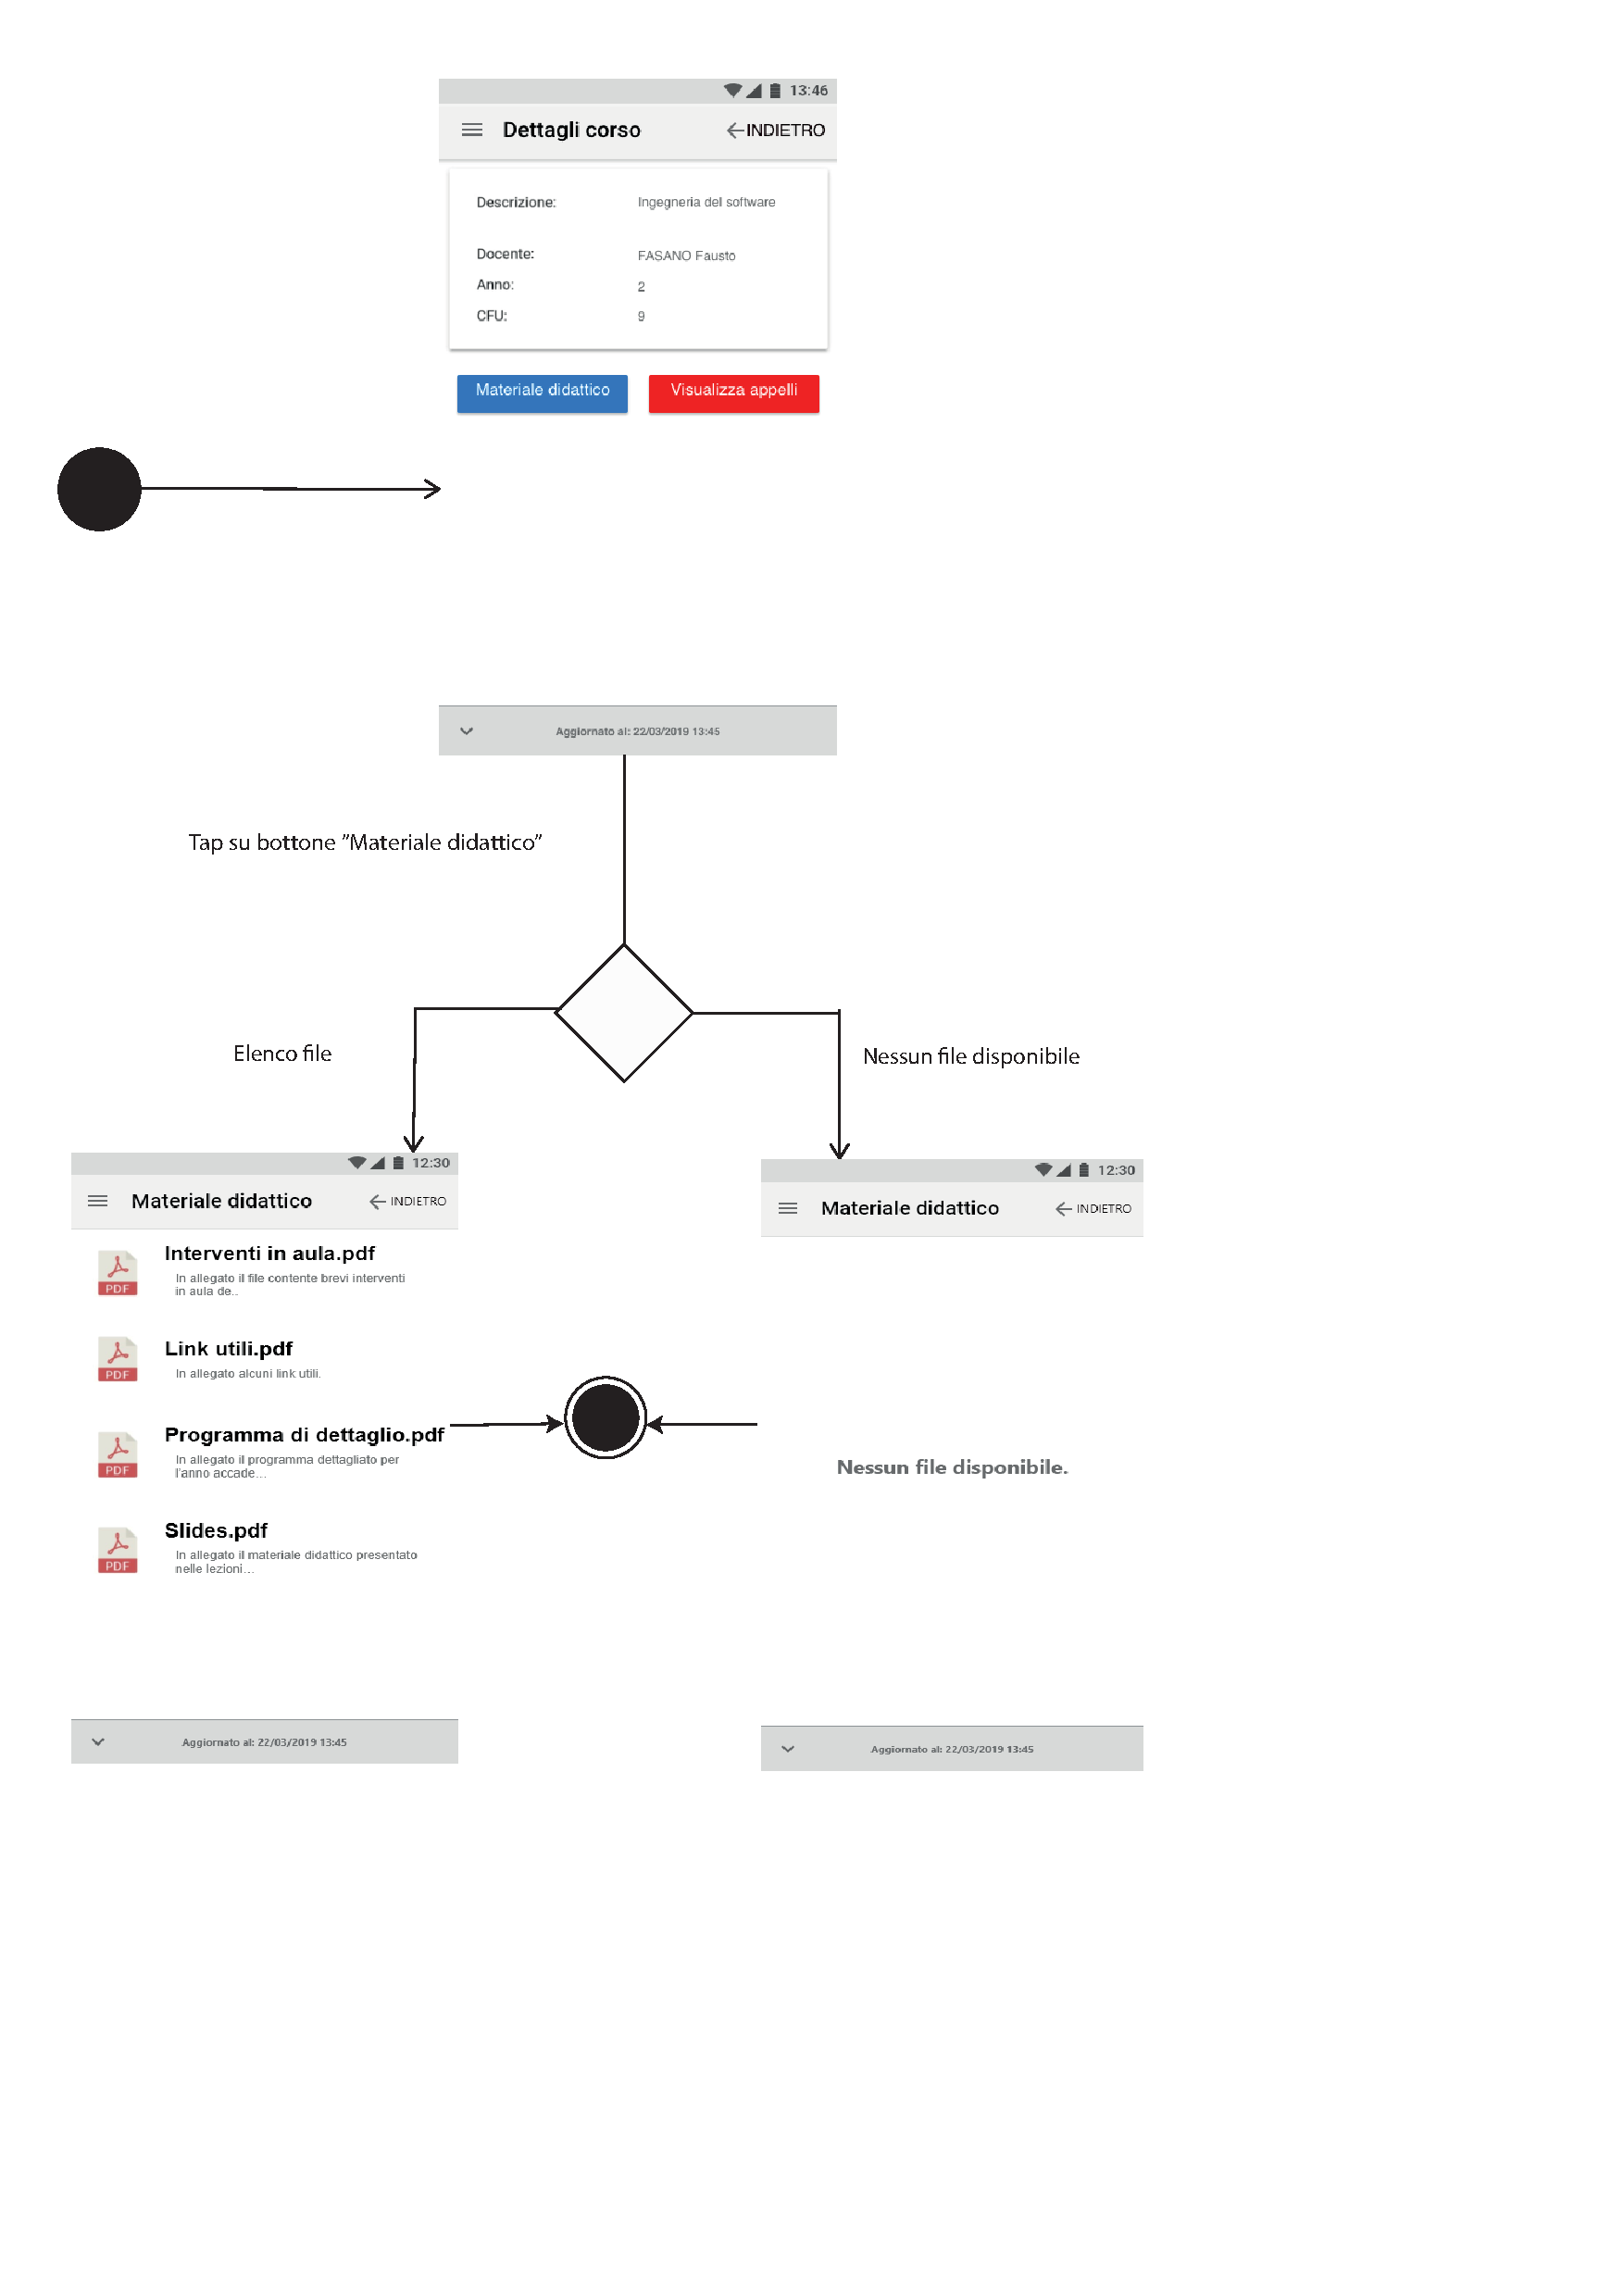
\includegraphics[width=6in]{imgs/gruppo1/activity_diagrams/AD13_viasualizza_elenco_file.pdf}
\end{center}
\newpage

%%8.6.14 - Ricerca files%%

\subsection{Ricerca files}
\begin{center}
	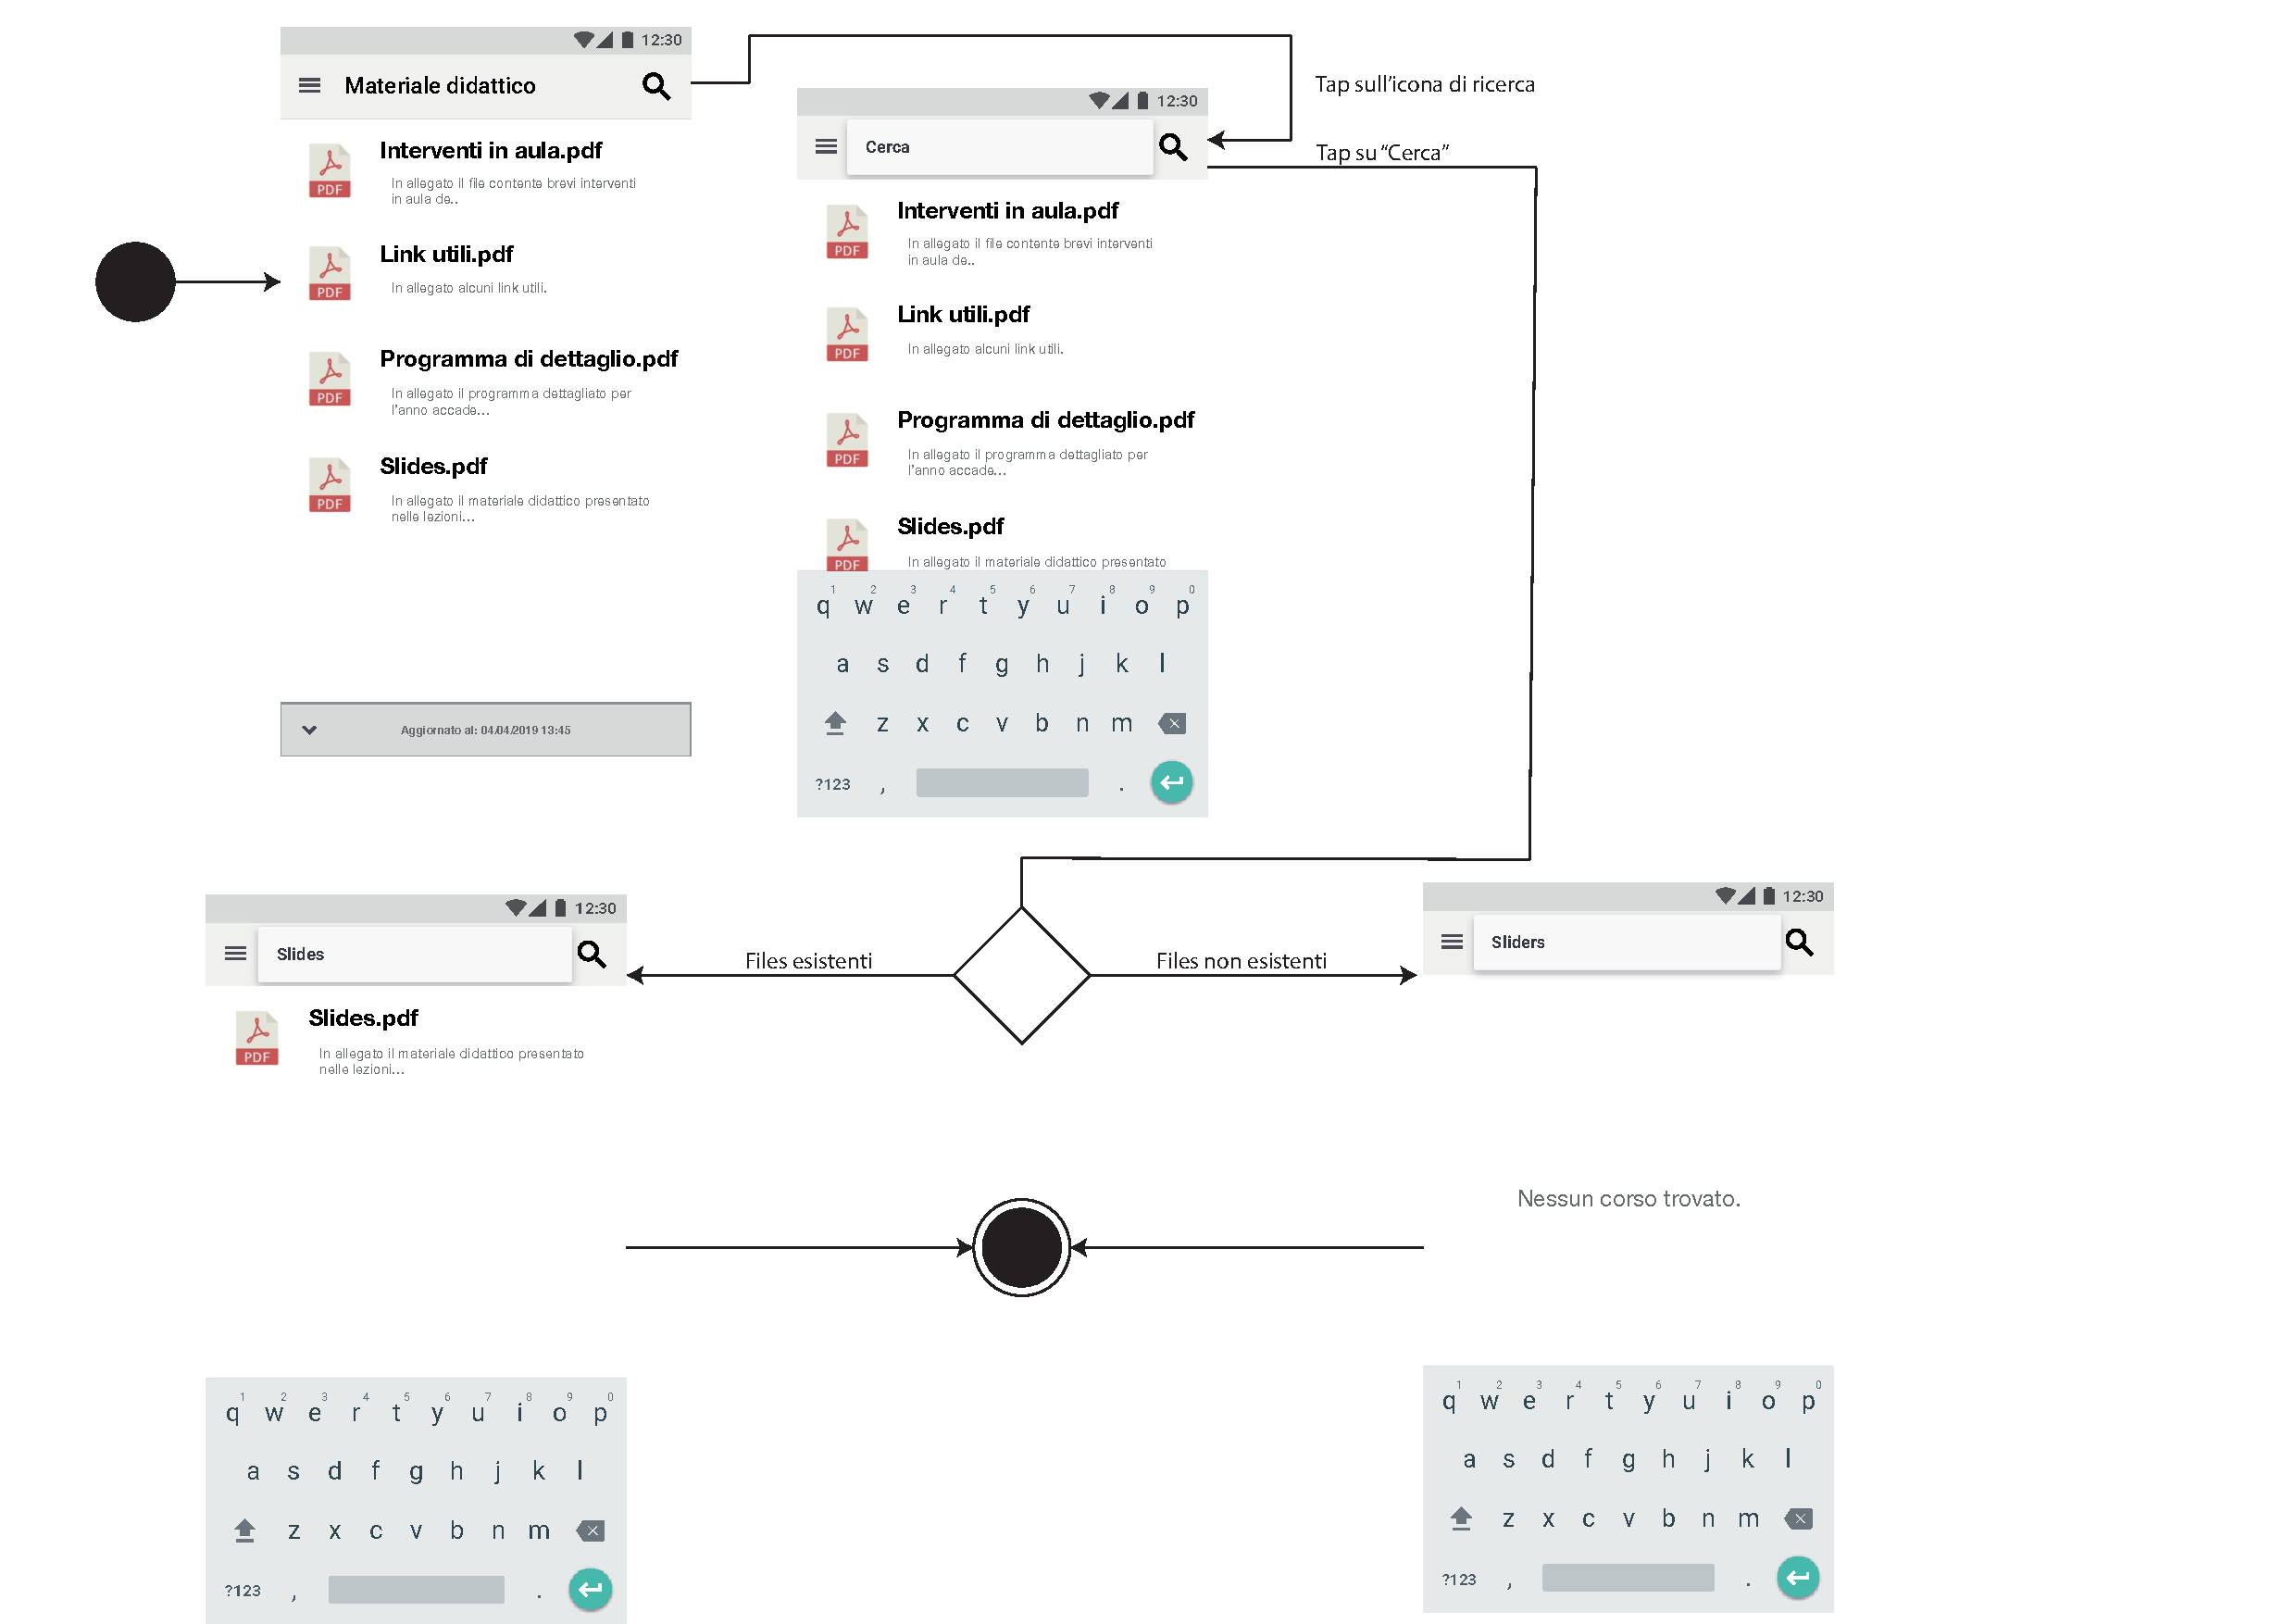
\includegraphics[width=6in]{imgs/gruppo1/activity_diagrams/AD14_ricerca_file.pdf}
\end{center}
\newpage

%%8.6.15 - Visualizza dettagli file%%

\subsection{Visualizza dettagli file}
\begin{center}
	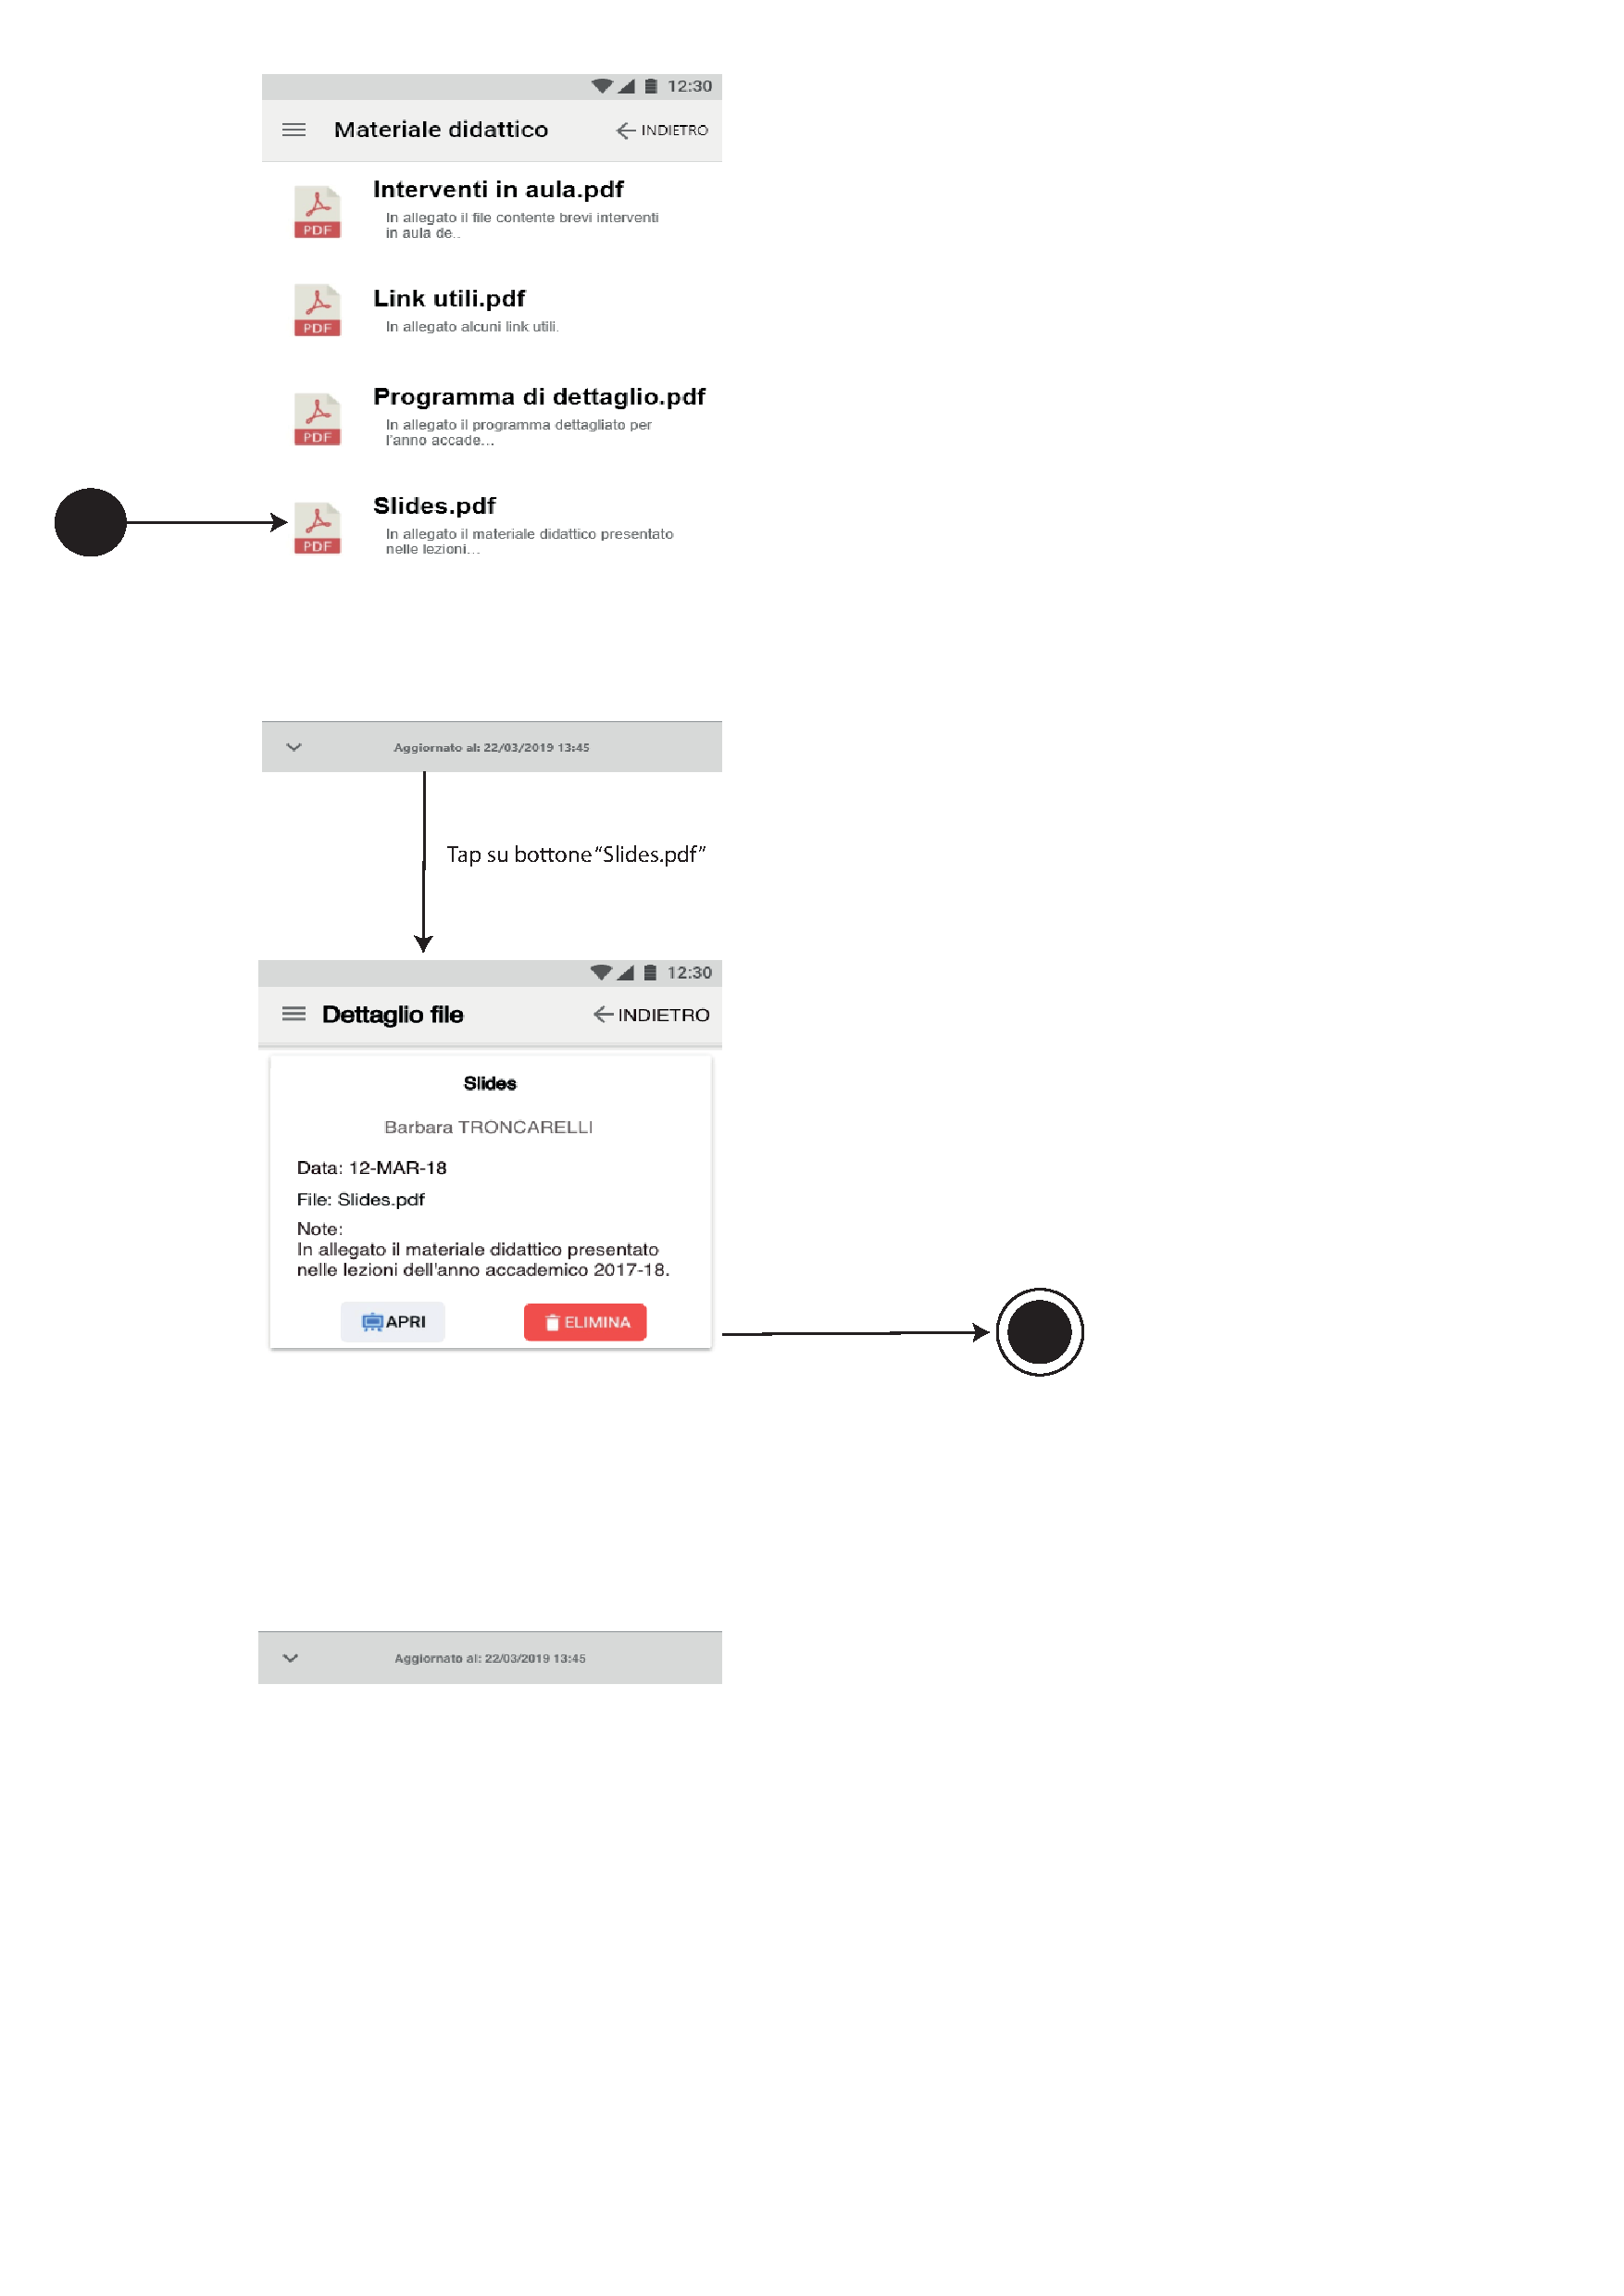
\includegraphics[width=6in]{imgs/gruppo1/activity_diagrams/AD15_dettagli_file.pdf}
\end{center}
\newpage

%%8.6.16 - Apri file%%

\subsection{Apri file}
\begin{center}
	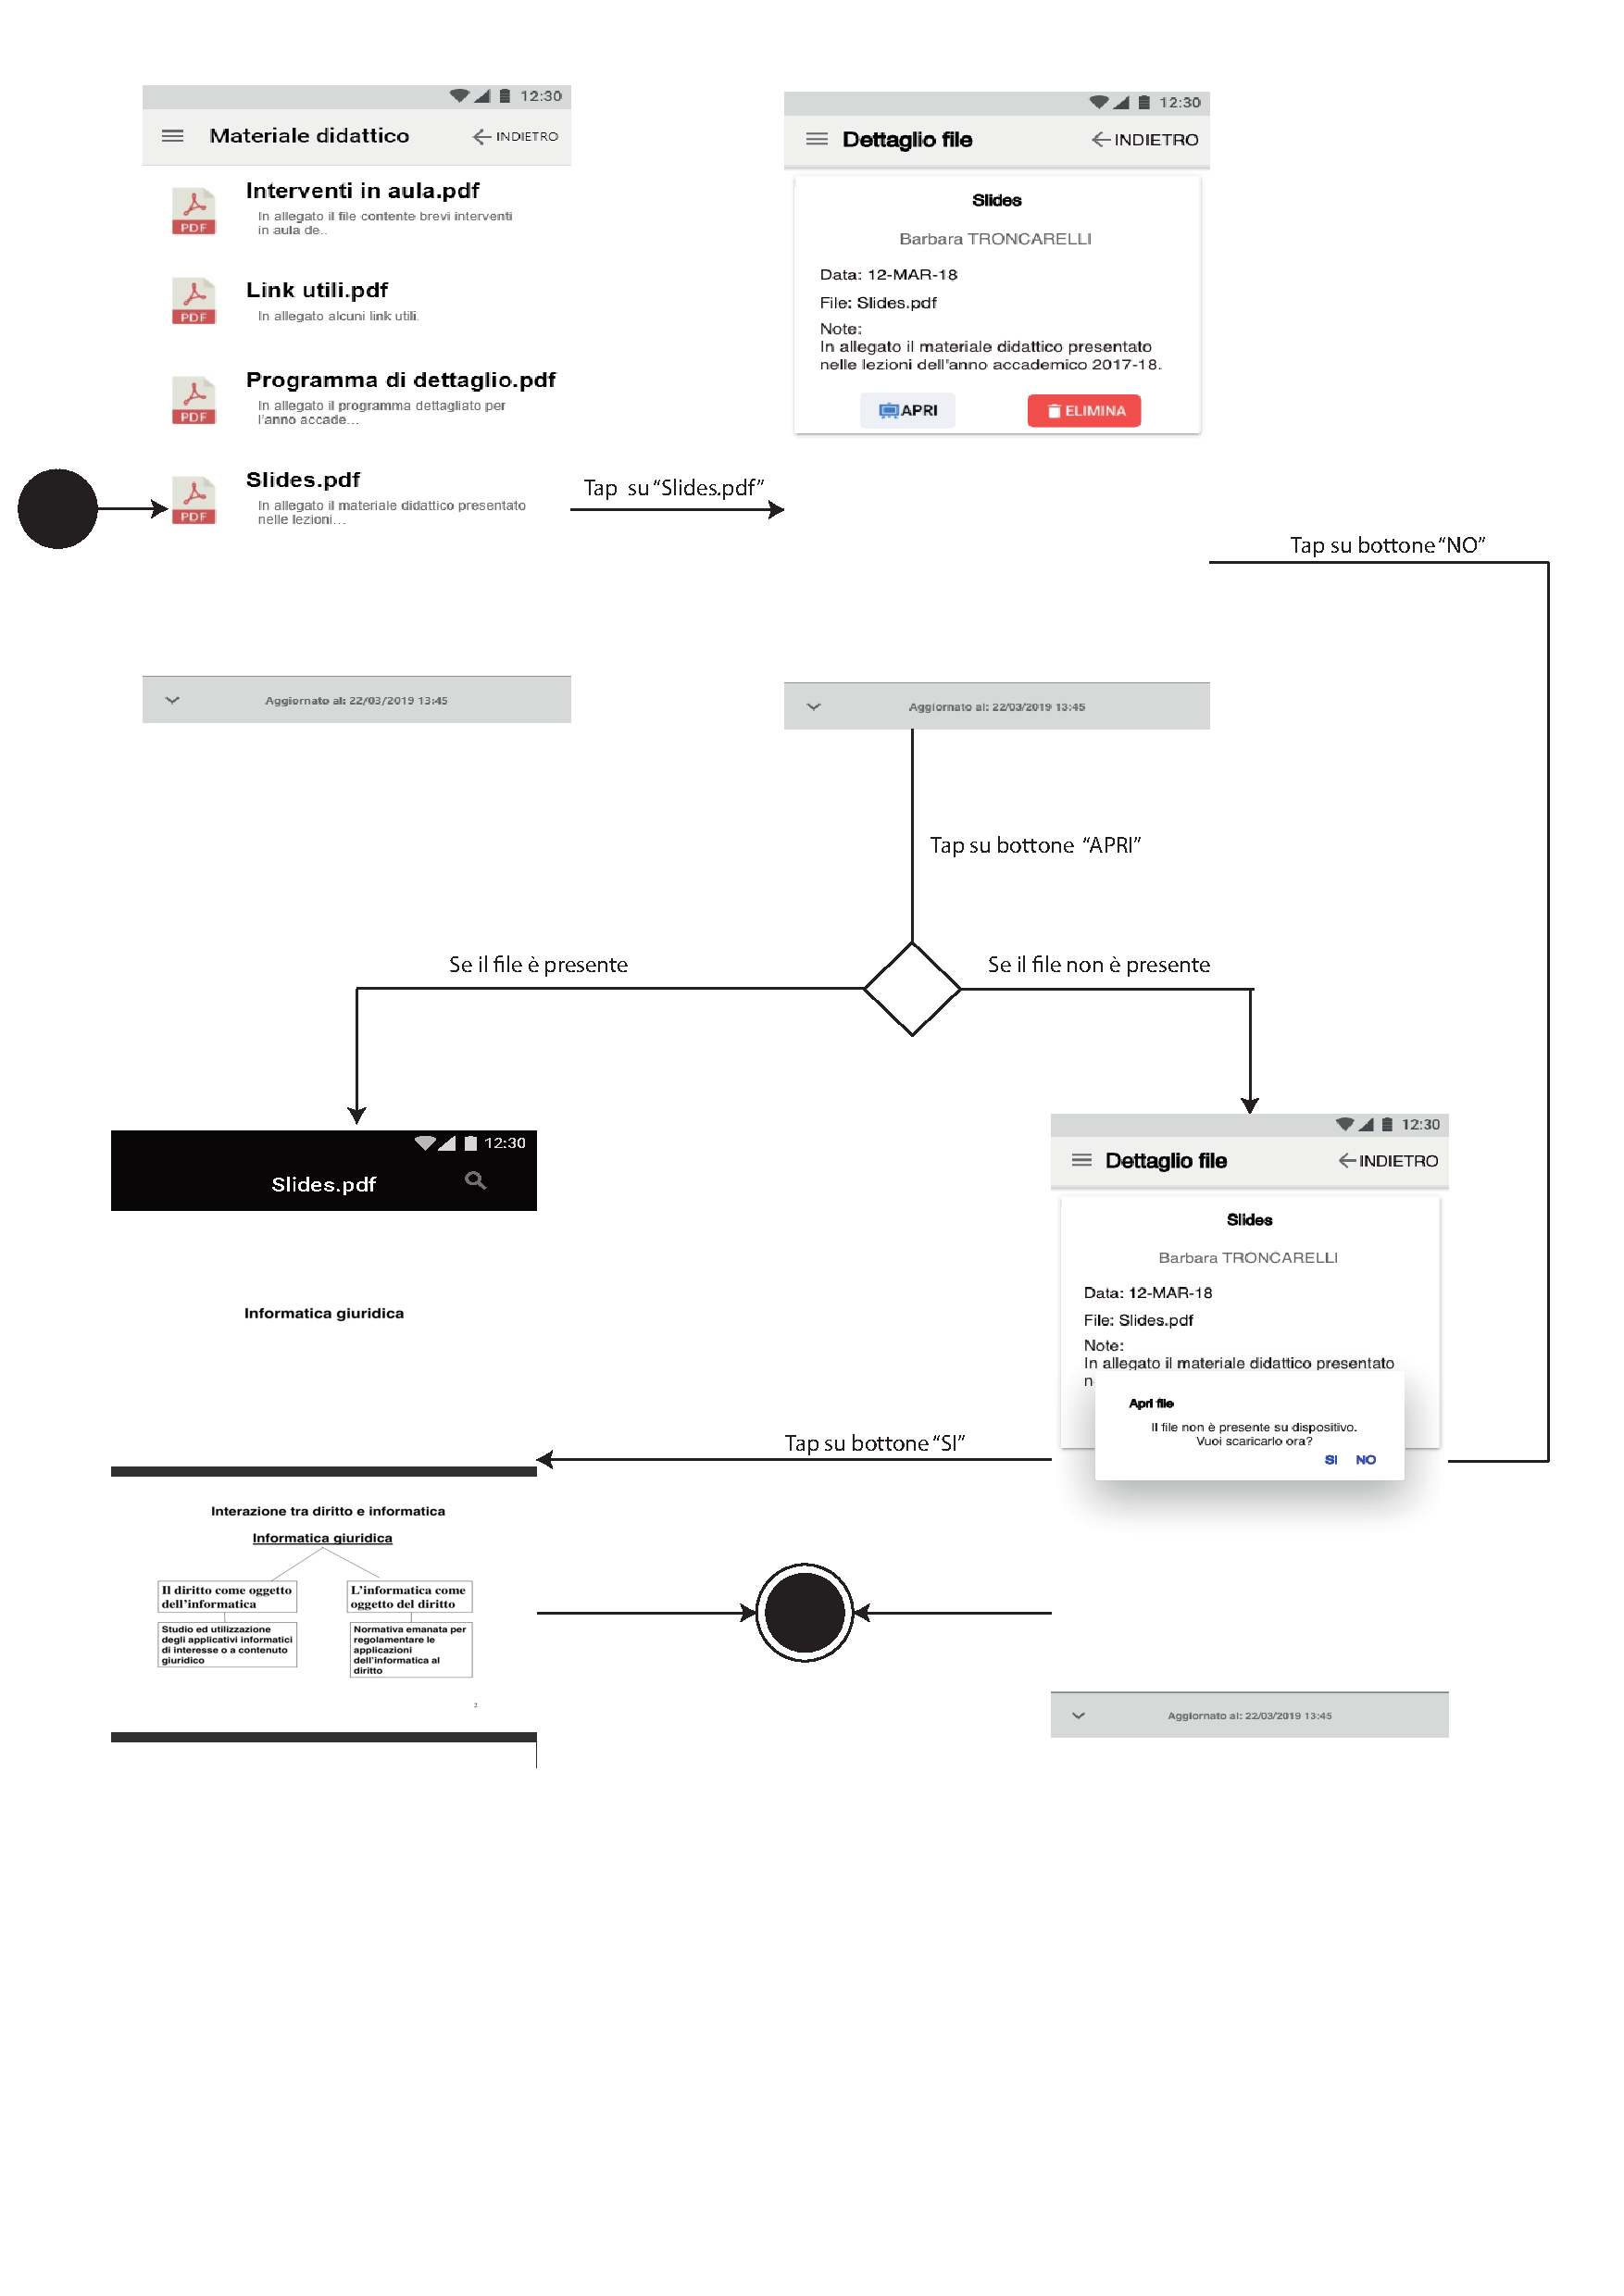
\includegraphics[width=6in]{imgs/gruppo1/activity_diagrams/AD16_apri_file.pdf}
\end{center}
\newpage

%%8.6.17 - Rimuovi file%%

\subsection{Rimuovi file}
\begin{center}
	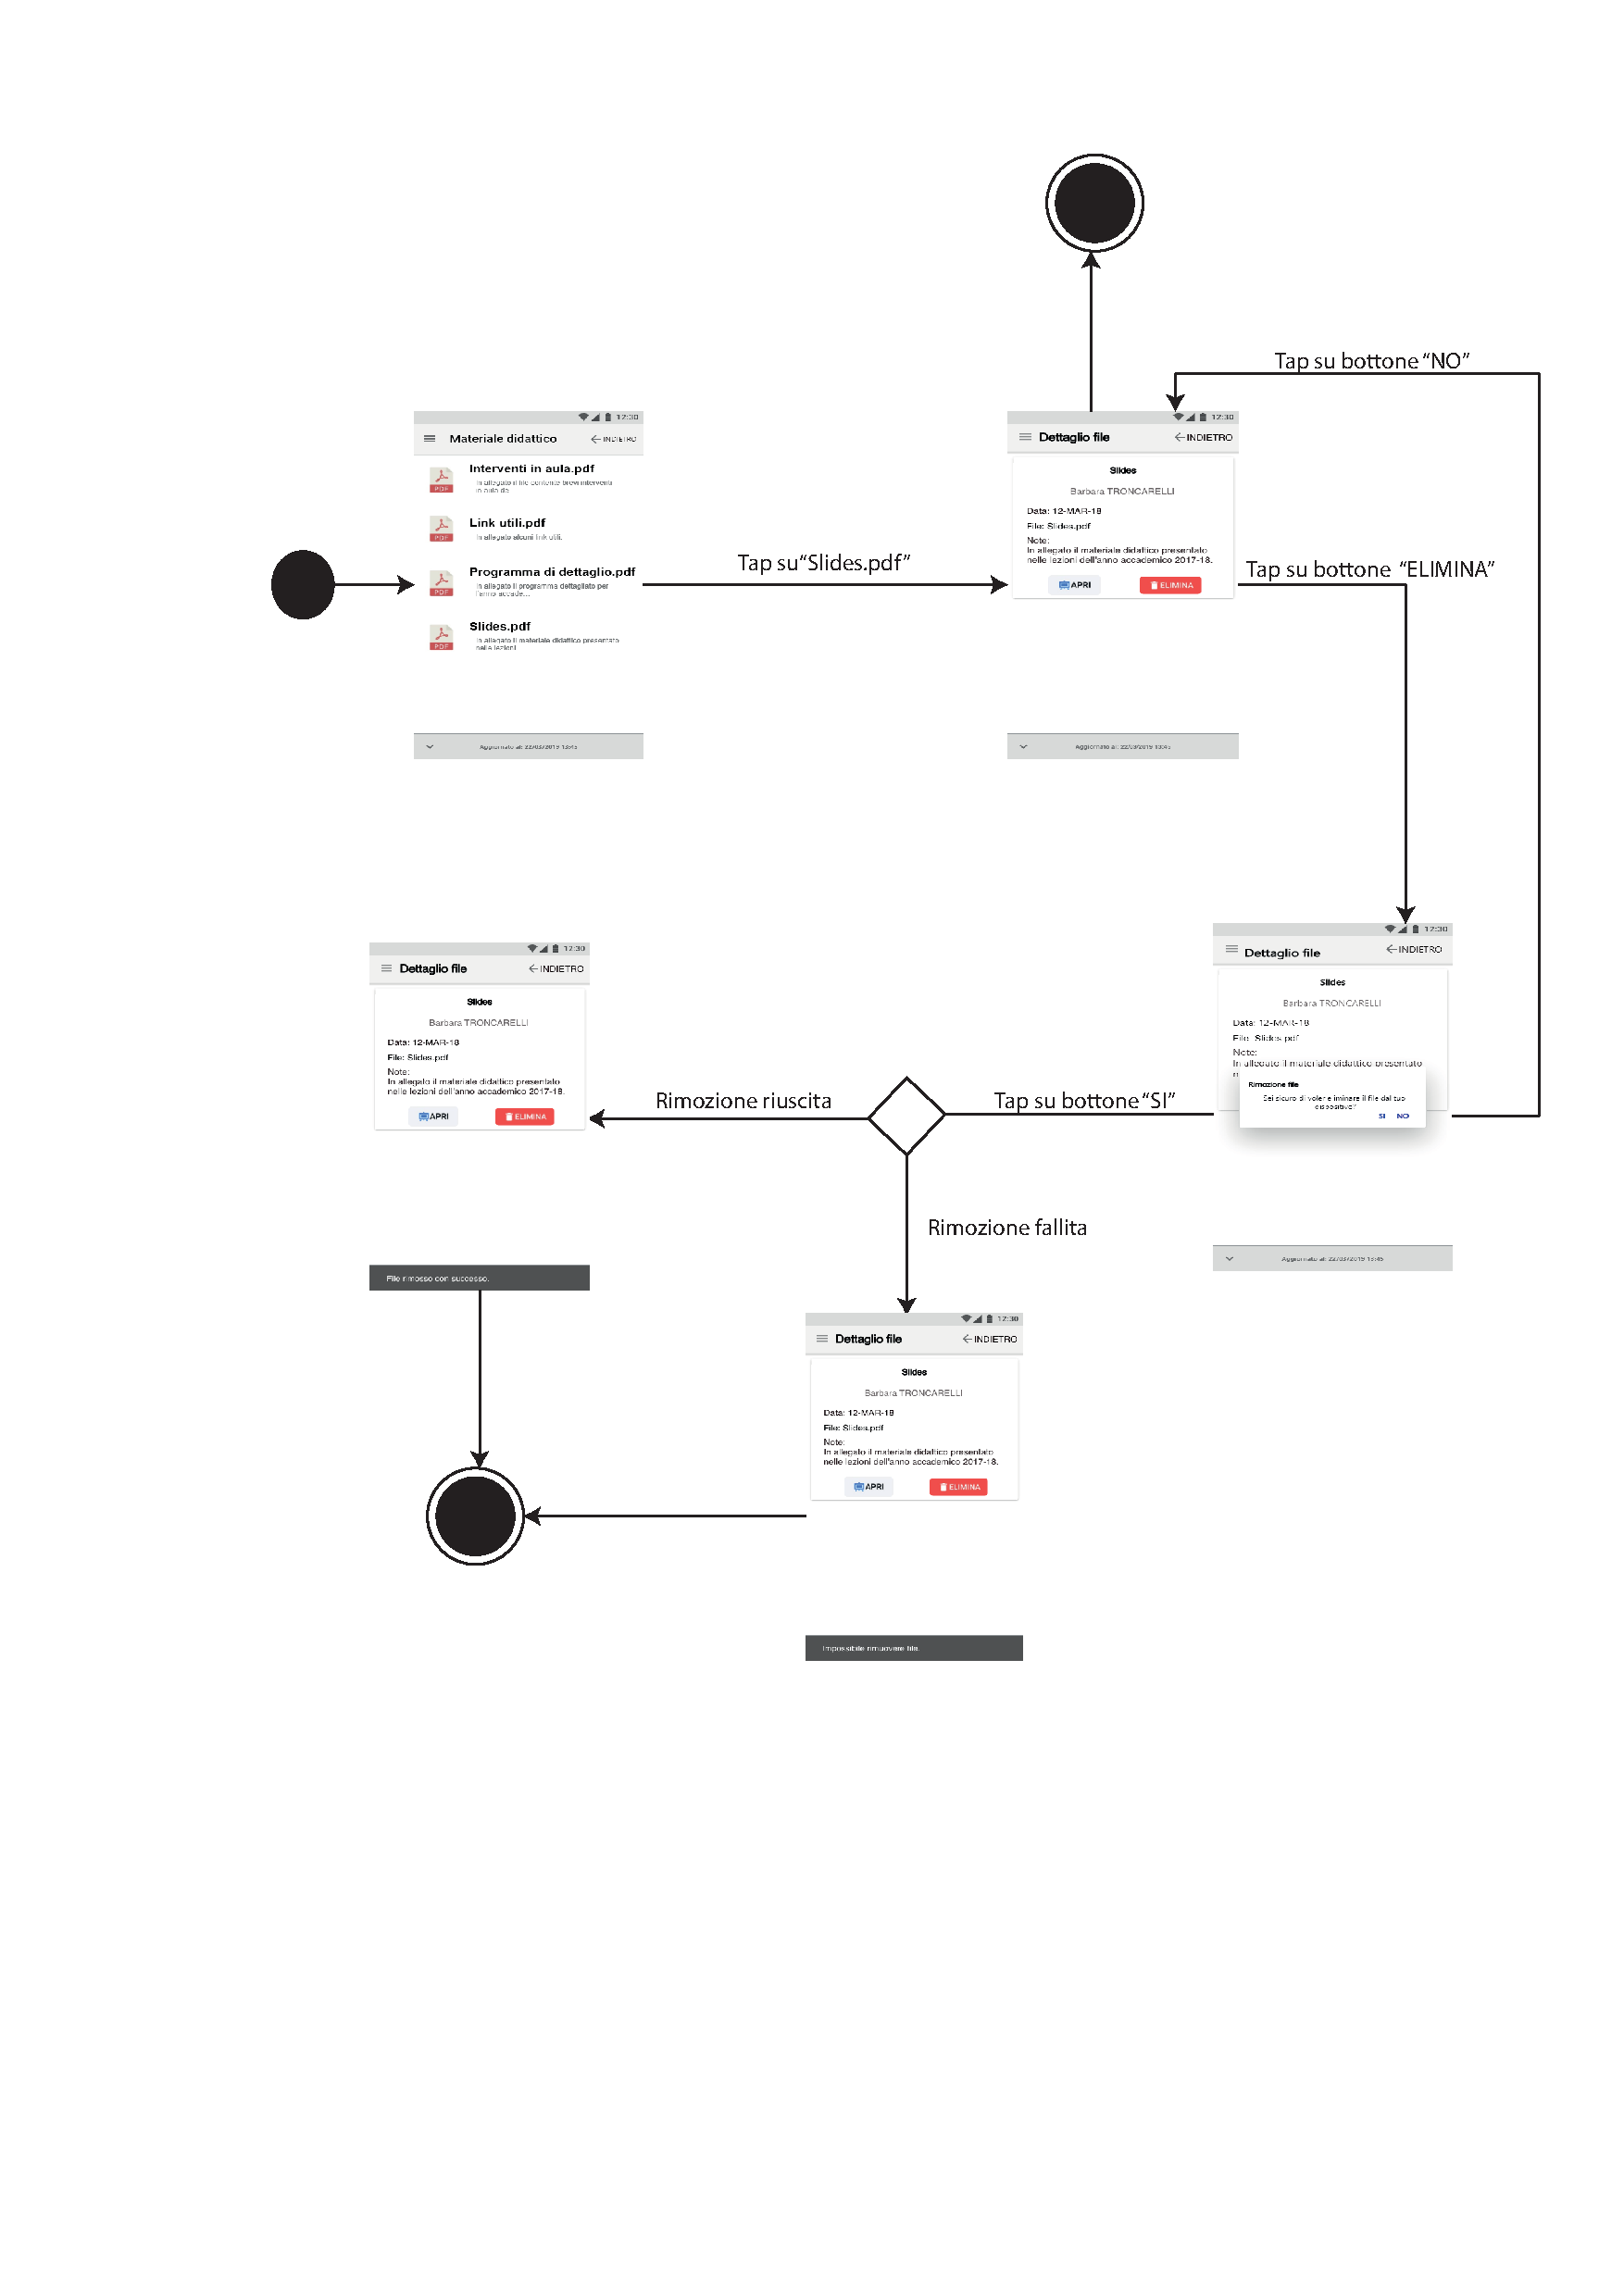
\includegraphics[width=6in]{imgs/gruppo1/activity_diagrams/AD17_rimuovi_file.pdf}
\end{center}
\newpage

	%%%%%%%%%%%%%%%%%%%%%%%%%%%%%%%%%%%%%%%%%%%%%%%%%%%%%%%%%%%

\chapter{Modello del sistema - gruppo 2}
\label{ref:modSistemaGruppo2}

%%% Il gruppo 2 scriverà il suo modello del sistema. Esso dovrà includere: attori, casi d'uso (descrizione e tabella), scenari, diagrammi dei casi d'uso, diagrammi di sequenza, diagramma delle attività, screen mockups della funzionalità %%%

\section{Attori}
Descrivere gli attori che partecipano ai seguenti caso d'uso.

\section{Scenari}
Inserire qui gli scenari che sono un'istanza dei casi d'uso: gli scenari danno dei valori al flusso degli eventi dei casi d'uso. Esempio di caso d'uso "visualizza libretto": l'utente Antonio - che ha effettuato il login con username "Antonio" e password "antonioilmigliore" - accede alla sezione "libretto" e visualizza gli esami sostenuti Programmazione e Inglese con le votazioni rispettive di 25 e 30.

\section{Casi d'uso}
Per ogni caso d'uso inserire descrizione e tabella. Se il tuo caso d'uso prevede più attori di quelli che sono nella tabella sottostante di esempio, aggiungi una colonna nella sezione flusso degli eventi!

\paragraph{Caso d'uso 1 (sostituire con nome caso d'uso) \\} 
Lorem ipsum dolor sit amet... (sostituire con descrizione caso d'uso)

\begin{table}[tb]
%\normalsize % Dimensione testo normale
\small % Dimensione testo piccola
%\footnotesize % Dimensione testo piccolissima
%\scriptsize % Dimensione del testo ulteriormente più piccola
%\caption{} % Didascalia tabella
%\label{} % Etichetta per riferimenti incrociati
\begin{tabular}{| p{\useCaseLeft} | p{\useCaseNum} | p{\useCaseTwoCol} | p{\useCaseTwoCol} |}
	\hline
	\textbf{Nome caso d'uso} & \multicolumn{3}{p{\useCaseMulticol} |}{\textbf{Login}} \\
	\hline
	\textbf{Attori partecipanti} & \multicolumn{3}{p{\useCaseMulticol} |}{Inizializzato da \textbf{Utente}.} \\
	\hline
	\textbf{Condizioni d'ingresso} & \multicolumn{3}{p{\useCaseMulticol} |}{L'utente ha cliccato sul bottone di login.} \\
	\hline
	\textbf{Flusso degli eventi} & \textbf{\#} & \textbf{Utente} & \textbf{Sistema} \\
	\hline
	\textbf{} & \textbf{1} & \textbf{} & Propone una schermata per l'inserimento dei dati necessari per il login, e-mail e password dell'utente \\
	\hline
	\textbf{} & \textbf{2} & Inserisce i dati e sottomette la richiesta & \textbf{} \\
	\hline
	\textbf{} & \textbf{3} & \textbf{} & Controlla che siano stati inseriti entrambi i campi e avvia le operazioni di visualizzazione \\
	\hline
	\textbf{Eccezioni} & \multicolumn{3}{p{\useCaseMulticol} |}{3.1 Uno o entrambi i campi sono vuoti.\newline 3.2 Le credenziali inserite non sono valide (una o entrambe).} \\
	\hline
	\textbf{Condizioni d'uscita} & \multicolumn{3}{p{\useCaseMulticol} |}{Il sistema completa la login e dà accesso all'app o, in caso contrario, visualizza un messaggio di errore se non sono stati inseriti tutti i dati obbligatori, se le credenziali non sono corrette o se si verifica un insuccesso dell'operazione.} \\
	\hline
\end{tabular}
\end{table}

\section{Diagramma dei casi d'uso}

Inserire immagine del diagramma. Le immagini vanno caricate nella cartella imgs, va inserito il path corrispondente (nomefile.estensione) dopo il tag includegraphics e va cambiata la descrizione dell'immagine (caption) con un'etichetta opportuna. Sostituire l'immagine file-comuni-ai-gruppi/useCaseEsempio.png con quella desiderata.

\begin{figure}
	\centering
	\includegraphics[height=3in]{imgs/file-comuni-ai-gruppi/useCaseEsempio.png}
	\caption{Inserire descrizione}
	\label{fig:prova}
\end{figure}

\section{Diagramma di sequenza}

Inserire immagine del diagramma. Le immagini vanno caricate nella cartella imgs, va inserito il path corrispondente (nomefile.estensione) dopo il tag includegraphics e va cambiata la descrizione dell'immagine (caption) con un'etichetta opportuna. Sostituire l'immagine file-comuni-ai-gruppi/useCaseEsempio.png con quella desiderata.

\begin{figure}
	\centering
	\includegraphics[height=3in,width=5in]{imgs/file-comuni-ai-gruppi/SequenceDgEsempio.png}
	\caption{Inserire descrizione}
	\label{fig:prova}
\end{figure}

\section{Diagramma delle attività}

Inserire immagine del diagramma. Le immagini vanno caricate nella cartella imgs, va inserito il path corrispondente (nomefile.estensione) dopo il tag includegraphics e va cambiata la descrizione dell'immagine (caption) con un'etichetta opportuna. Sostituire l'immagine file-comuni-ai-gruppi/useCaseEsempio.png con quella desiderata.

\begin{figure}
	\centering
	\includegraphics[height=3in,width=5in]{imgs/file-comuni-ai-gruppi/ActivityDgEsempio.png}
	\caption{Inserire descrizione}
	\label{fig:prova}
\end{figure}

\clearpage
	%%%%%%%%%%%%%%%%%%%%%%%%%%%%%%%%%%%%%%%%%%%%%%%%%%%%%%%%%%%

\chapter{Modello del sistema - gruppo 3}
\label{ref:modSistemaGruppo3}

%%% Il gruppo 3 scriverà il suo modello del sistema. Esso dovrà includere: attori, casi d'uso (descrizione e tabella), scenari, diagrammi dei casi d'uso, diagrammi di sequenza, diagramma delle attività, screen mockups della funzionalità %%%

\section{Attori}
Descrivere gli attori che partecipano ai seguenti caso d'uso.

\section{Casi d'uso}
Per ogni caso d'uso inserire descrizione e tabella. Se il tuo caso d'uso prevede più attori di quelli che sono nella tabella sottostante di esempio, aggiungi una colonna nella sezione flusso degli eventi!

\paragraph{Caso d'uso 1 (sostituire con nome caso d'uso) \\} 
Lorem ipsum dolor sit amet... (sostituire con descrizione caso d'uso)

\begin{table}[tb]
%\normalsize % Dimensione testo normale
\small % Dimensione testo piccola
%\footnotesize % Dimensione testo piccolissima
%\scriptsize % Dimensione del testo ulteriormente più piccola
%\caption{} % Didascalia tabella
%\label{} % Etichetta per riferimenti incrociati
\begin{tabular}{| p{\useCaseLeft} | p{\useCaseNum} | p{\useCaseTwoCol} | p{\useCaseTwoCol} |}
	\hline
	\textbf{Nome caso d'uso} & \multicolumn{3}{p{\useCaseMulticol} |}{\textbf{Login}} \\
	\hline
	\textbf{Attori partecipanti} & \multicolumn{3}{p{\useCaseMulticol} |}{Inizializzato da \textbf{Utente}.} \\
	\hline
	\textbf{Condizioni d'ingresso} & \multicolumn{3}{p{\useCaseMulticol} |}{L'utente ha cliccato sul bottone di login.} \\
	\hline
	\textbf{Flusso degli eventi} & \textbf{\#} & \textbf{Utente} & \textbf{Sistema} \\
	\hline
	\textbf{} & \textbf{1} & \textbf{} & Propone una schermata per l'inserimento dei dati necessari per il login, e-mail e password dell'utente \\
	\hline
	\textbf{} & \textbf{2} & Inserisce i dati e sottomette la richiesta & \textbf{} \\
	\hline
	\textbf{} & \textbf{3} & \textbf{} & Controlla che siano stati inseriti entrambi i campi e avvia le operazioni di visualizzazione \\
	\hline
	\textbf{Eccezioni} & \multicolumn{3}{p{\useCaseMulticol} |}{3.1 Uno o entrambi i campi sono vuoti.\newline 3.2 Le credenziali inserite non sono valide (una o entrambe).} \\
	\hline
	\textbf{Condizioni d'uscita} & \multicolumn{3}{p{\useCaseMulticol} |}{Il sistema completa la login e dà accesso all'app o, in caso contrario, visualizza un messaggio di errore se non sono stati inseriti tutti i dati obbligatori, se le credenziali non sono corrette o se si verifica un insuccesso dell'operazione.} \\
	\hline
\end{tabular}
\end{table}

\section{Diagramma dei casi d'uso}

Inserire immagine del diagramma. Le immagini vanno caricate nella cartella imgs, va inserito il path corrispondente (nomefile.estensione) dopo il tag includegraphics e va cambiata la descrizione dell'immagine (caption) con un'etichetta opportuna. Sostituire l'immagine file-comuni-ai-gruppi/useCaseEsempio.png con quella desiderata.

\begin{figure}
	\centering
	\includegraphics[height=3in]{imgs/file-comuni-ai-gruppi/useCaseEsempio.png}
	\caption{Inserire descrizione}
	\label{fig:prova}
\end{figure}

\section{Scenari}
Inserire qui gli scenari che sono un'istanza dei casi d'uso: gli scenari danno dei valori al flusso degli eventi dei casi d'uso. Esempio di caso d'uso "visualizza libretto": l'utente Antonio - che ha effettuato il login con username "Antonio" e password "antonioilmigliore" - accede alla sezione "libretto" e visualizza gli esami sostenuti Programmazione e Inglese con le votazioni rispettive di 25 e 30.

\section{Diagramma di sequenza}

Inserire immagine del diagramma. Le immagini vanno caricate nella cartella imgs, va inserito il path corrispondente (nomefile.estensione) dopo il tag includegraphics e va cambiata la descrizione dell'immagine (caption) con un'etichetta opportuna. Sostituire l'immagine file-comuni-ai-gruppi/useCaseEsempio.png con quella desiderata.

\begin{figure}
	\centering
	\includegraphics[height=3in,width=5in]{imgs/file-comuni-ai-gruppi/SequenceDgEsempio.png}
	\caption{Inserire descrizione}
	\label{fig:prova}
\end{figure}

\section{Diagramma delle attività}

Inserire immagine del diagramma. Le immagini vanno caricate nella cartella imgs, va inserito il path corrispondente (nomefile.estensione) dopo il tag includegraphics e va cambiata la descrizione dell'immagine (caption) con un'etichetta opportuna. Sostituire l'immagine file-comuni-ai-gruppi/useCaseEsempio.png con quella desiderata.

\begin{figure}
	\centering
	\includegraphics[height=3in,width=5in]{imgs/file-comuni-ai-gruppi/ActivityDgEsempio.png}
	\caption{Inserire descrizione}
	\label{fig:prova}
\end{figure}

\section{Screen mockups}

Inserire immagine degli screen della funzionalità. Le immagini vanno caricate nella cartella imgs, va inserito il path corrispondente (nomefile.estensione) dopo il tag includegraphics e va cambiata la descrizione dell'immagine (caption) con un'etichetta opportuna. Sostituire l'immagine file-comuni-ai-gruppi/useCaseEsempio.png con quella desiderata.

\begin{figure}
	\centering
	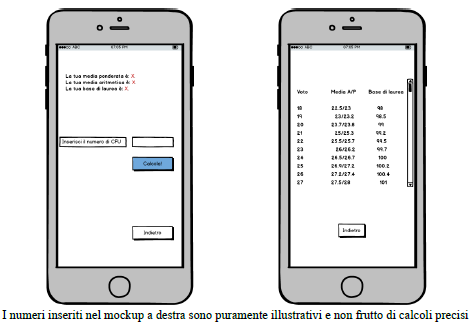
\includegraphics[height=3in]{imgs/file-comuni-ai-gruppi/MockupEsempio.png}
	\caption{Inserire descrizione}
	\label{fig:prova}
\end{figure}

\clearpage
	%%%%%%%%%%%%%%%%%%%%%%%%%%%%%%%%%%%%%%%%%%%%%%%%%%%%%%%%%%%

\chapter{Modello del sistema - gruppo 4}
\label{ref:modSistemaGruppo4}

%%% Il gruppo 4 scriverà il suo modello del sistema. Esso dovrà includere: attori, casi d'uso (descrizione e tabella), scenari, diagrammi dei casi d'uso, diagrammi di sequenza, diagramma delle attività, screen mockups della funzionalità %%%

\section{Attori}
Descrivere gli attori che partecipano ai seguenti caso d'uso.

\section{Casi d'uso}
Per ogni caso d'uso inserire descrizione e tabella. Se il tuo caso d'uso prevede più attori di quelli che sono nella tabella sottostante di esempio, aggiungi una colonna nella sezione flusso degli eventi!

\paragraph{Caso d'uso 1 (sostituire con nome caso d'uso) \\} 
Lorem ipsum dolor sit amet... (sostituire con descrizione caso d'uso)

\begin{table}[tb]
\normalsize % Dimensione testo normale
%\small % Dimensione testo piccola
%\footnotesize % Dimensione testo piccolissima
%\caption{} % Didascalia tabella
%\label{} % Etichetta per riferimenti incrociati
\begin{tabular}{| p{0.20\textwidth} | p{0.05\textwidth} | p{0.35\textwidth} | p{0.35\textwidth} |}
	\hline
	\textbf{Nome caso d'uso} & \multicolumn{3}{| p{0.75\textwidth} |}{\textbf{Login}} \\
	\hline
	\textbf{Attori partecipanti} & \multicolumn{3}{| p{0.75\textwidth} |}{Inizializzato da \textbf{Utente}.} \\
	\hline
	\textbf{Condizioni d'ingresso} & \multicolumn{3}{| p{0.75\textwidth} |}{L'utente ha cliccato sul bottone di login.} \\
	\hline
	\textbf{Flusso degli eventi} & \textbf{\#} & \textbf{Utente} & \textbf{Sistema} \\
	\hline
	\textbf{} & \textbf{1} & \textbf{} & Propone una schermata per l'inserimento dei dati necessari per il login, e-mail e password dell'utente \\
	\hline
	\textbf{} & \textbf{2} & Inserisce i dati e sottomette la richiesta & \textbf{} \\
	\hline
	\textbf{} & \textbf{3} & \textbf{} & Controlla che siano stati inseriti entrambi i campi e avvia le operazioni di visualizzazione \\
	\hline
	\textbf{Eccezioni} & \multicolumn{3}{| p{0.75\textwidth} |}{3.1 Uno o entrambi i campi sono vuoti.\newline 3.2 Le credenziali inserite non sono valide (una o entrambe).} \\
	\hline
	\textbf{Condizioni d'uscita} & \multicolumn{3}{| p{0.75\textwidth} |}{Il sistema completa la login e d\`{a} accesso all'app o, in caso contrario, visualizza un messaggio di errore se non sono stati inseriti tutti i dati obbligatori, se le credenziali non sono corrette o se si verifica un insuccesso dell'operazione.} \\
	\hline
\end{tabular}
\end{table}

\section{Diagramma dei casi d'uso}

Inserire immagine del diagramma. Le immagini vanno caricate nella cartella imgs, va inserito il path corrispondente (nomefile.estensione) dopo il tag includegraphics e va cambiata la descrizione dell'immagine (caption) con un'etichetta opportuna. Sostituire l'immagine useCaseEsempio.PNG con quella desiderata.

\begin{figure}[H]
	\centering
	\includegraphics[height=3in]{imgs/useCaseEsempio.PNG}
	\caption{Inserire descrizione}
	\label{fig:prova}
\end{figure}

\section{Scenari}
Inserire qui gli scenari che sono un'istanza dei casi d'uso: gli scenari danno dei valori al flusso degli eventi dei casi d'uso. Esempio di caso d'uso "visualizza libretto": l'utente Antonio - che ha effettuato il login con username "Antonio" e password "antonioilmigliore" - accede alla sezione "libretto" e visualizza gli esami sostenuti Programmazione e Inglese con le votazioni rispettive di 25 e 30.

\section{Diagramma di sequenza}

Inserire immagine del diagramma. Le immagini vanno caricate nella cartella imgs, va inserito il path corrispondente (nomefile.estensione) dopo il tag includegraphics e va cambiata la descrizione dell'immagine (caption) con un'etichetta opportuna. Sostituire l'immagine useCaseEsempio.PNG con quella desiderata.

\begin{figure}[H]
	\centering
	\includegraphics[height=3in,width=5in]{imgs/SequenceDgEsempio.PNG}
	\caption{Inserire descrizione}
	\label{fig:prova}
\end{figure}

\section{Diagramma delle attività}

Inserire immagine del diagramma. Le immagini vanno caricate nella cartella imgs, va inserito il path corrispondente (nomefile.estensione) dopo il tag includegraphics e va cambiata la descrizione dell'immagine (caption) con un'etichetta opportuna. Sostituire l'immagine useCaseEsempio.PNG con quella desiderata.

\begin{figure}[H]
	\centering
	\includegraphics[height=3in,width=5in]{imgs/ActivityDgEsempio.PNG}
	\caption{Inserire descrizione}
	\label{fig:prova}
\end{figure}

\section{Screen mockups}

Inserire immagine degli screen della funzionalità. Le immagini vanno caricate nella cartella imgs, va inserito il path corrispondente (nomefile.estensione) dopo il tag includegraphics e va cambiata la descrizione dell'immagine (caption) con un'etichetta opportuna. Sostituire l'immagine useCaseEsempio.PNG con quella desiderata.

\begin{figure}[H]
	\centering
	\includegraphics[height=3in]{imgs/MockupEsempio.PNG}
	\caption{Inserire descrizione}
	\label{fig:prova}
\end{figure}

\newpage
	%%%%%%%%%%%%%%%%%%%%%%%%%%%%%%%%%%%%%%%%%%%%%%%%%%%%%%%%%%%

\chapter{Modello del sistema - gruppo 5}
\label{ref:modSistemaGruppo5}

%%% Il gruppo 5 scriverà il suo modello del sistema. Esso dovrà includere: attori, casi d'uso (descrizione e tabella), scenari, diagrammi dei casi d'uso, diagrammi di sequenza, diagramma delle attività, screen mockups della funzionalità %%%

\section{Attori}
Descrivere gli attori che partecipano ai seguenti caso d'uso.

\section{Casi d'uso}
Per ogni caso d'uso inserire descrizione e tabella. Se il tuo caso d'uso prevede più attori di quelli che sono nella tabella sottostante di esempio, aggiungi una colonna nella sezione flusso degli eventi!

\paragraph{Caso d'uso 1 (sostituire con nome caso d'uso) \\} 
Lorem ipsum dolor sit amet... (sostituire con descrizione caso d'uso)

\begin{table}[tb]
\normalsize % Dimensione testo normale
%\small % Dimensione testo piccola
%\footnotesize % Dimensione testo piccolissima
%\caption{} % Didascalia tabella
%\label{} % Etichetta per riferimenti incrociati
\begin{tabular}{| p{0.20\textwidth} | p{0.05\textwidth} | p{0.35\textwidth} | p{0.35\textwidth} |}
	\hline
	\textbf{Nome caso d'uso} & \multicolumn{3}{| p{0.75\textwidth} |}{\textbf{Login}} \\
	\hline
	\textbf{Attori partecipanti} & \multicolumn{3}{| p{0.75\textwidth} |}{Inizializzato da \textbf{Utente}.} \\
	\hline
	\textbf{Condizioni d'ingresso} & \multicolumn{3}{| p{0.75\textwidth} |}{L'utente ha cliccato sul bottone di login.} \\
	\hline
	\textbf{Flusso degli eventi} & \textbf{\#} & \textbf{Utente} & \textbf{Sistema} \\
	\hline
	\textbf{} & \textbf{1} & \textbf{} & Propone una schermata per l'inserimento dei dati necessari per il login, e-mail e password dell'utente \\
	\hline
	\textbf{} & \textbf{2} & Inserisce i dati e sottomette la richiesta & \textbf{} \\
	\hline
	\textbf{} & \textbf{3} & \textbf{} & Controlla che siano stati inseriti entrambi i campi e avvia le operazioni di visualizzazione \\
	\hline
	\textbf{Eccezioni} & \multicolumn{3}{| p{0.75\textwidth} |}{3.1 Uno o entrambi i campi sono vuoti.\newline 3.2 Le credenziali inserite non sono valide (una o entrambe).} \\
	\hline
	\textbf{Condizioni d'uscita} & \multicolumn{3}{| p{0.75\textwidth} |}{Il sistema completa la login e d\`{a} accesso all'app o, in caso contrario, visualizza un messaggio di errore se non sono stati inseriti tutti i dati obbligatori, se le credenziali non sono corrette o se si verifica un insuccesso dell'operazione.} \\
	\hline
\end{tabular}
\end{table}

\section{Diagramma dei casi d'uso}

Inserire immagine del diagramma. Le immagini vanno caricate nella cartella imgs, va inserito il path corrispondente (nomefile.estensione) dopo il tag includegraphics e va cambiata la descrizione dell'immagine (caption) con un'etichetta opportuna. Sostituire l'immagine file-comuni-ai-gruppi/useCaseEsempio.png con quella desiderata.

\begin{figure}[H]
	\centering
	\includegraphics[height=3in]{imgs/file-comuni-ai-gruppi/useCaseEsempio.png}
	\caption{Inserire descrizione}
	\label{fig:prova}
\end{figure}

\section{Scenari}
Inserire qui gli scenari che sono un'istanza dei casi d'uso: gli scenari danno dei valori al flusso degli eventi dei casi d'uso. Esempio di caso d'uso "visualizza libretto": l'utente Antonio - che ha effettuato il login con username "Antonio" e password "antonioilmigliore" - accede alla sezione "libretto" e visualizza gli esami sostenuti Programmazione e Inglese con le votazioni rispettive di 25 e 30.

\section{Diagramma di sequenza}

Inserire immagine del diagramma. Le immagini vanno caricate nella cartella imgs, va inserito il path corrispondente (nomefile.estensione) dopo il tag includegraphics e va cambiata la descrizione dell'immagine (caption) con un'etichetta opportuna. Sostituire l'immagine file-comuni-ai-gruppi/useCaseEsempio.png con quella desiderata.

\begin{figure}[H]
	\centering
	\includegraphics[height=3in,width=5in]{imgs/file-comuni-ai-gruppi/SequenceDgEsempio.png}
	\caption{Inserire descrizione}
	\label{fig:prova}
\end{figure}

\section{Diagramma delle attività}

Inserire immagine del diagramma. Le immagini vanno caricate nella cartella imgs, va inserito il path corrispondente (nomefile.estensione) dopo il tag includegraphics e va cambiata la descrizione dell'immagine (caption) con un'etichetta opportuna. Sostituire l'immagine file-comuni-ai-gruppi/useCaseEsempio.png con quella desiderata.

\begin{figure}[H]
	\centering
	\includegraphics[height=3in,width=5in]{imgs/file-comuni-ai-gruppi/ActivityDgEsempio.png}
	\caption{Inserire descrizione}
	\label{fig:prova}
\end{figure}

\section{Screen mockups}

Inserire immagine degli screen della funzionalità. Le immagini vanno caricate nella cartella imgs, va inserito il path corrispondente (nomefile.estensione) dopo il tag includegraphics e va cambiata la descrizione dell'immagine (caption) con un'etichetta opportuna. Sostituire l'immagine file-comuni-ai-gruppi/useCaseEsempio.png con quella desiderata.

\begin{figure}[H]
	\centering
	\includegraphics[height=3in]{imgs/file-comuni-ai-gruppi/MockupEsempio.png}
	\caption{Inserire descrizione}
	\label{fig:prova}
\end{figure}

\newpage
	%%%%%%%%%%%%%%%%%%%%%%%%%%%%%%%%%%%%%%%%%%%%%%%%%%%%%%%%%%%

\chapter{Modello del sistema - gruppo 6}
\label{ref:modSistemaGruppo6}

%%% Il gruppo 6 scriverà il suo modello del sistema. Esso dovrà includere: attori, casi d'uso (descrizione e tabella), scenari, diagrammi dei casi d'uso, diagrammi di sequenza, diagramma delle attività, screen mockups della funzionalità %%%

\section{Attori}
Descrivere gli attori che partecipano ai seguenti caso d'uso.

%%%%%%%%%%%%%%%PER QUANTO RIGUARDA IL NOSTRO ATTORE STUDENTE, VERRà INTEGRATO CON QUELLO DI TUTTI FACENDO UNA REF AD UNA LABEL
%N.B.:
%Per quanto riguarda la funzionalità chat \ref{nome-label} l'attore %studente ha in aggiunta le seguenti caratteristiche: ...

\section{Scenari}
Inserire qui gli scenari che sono un'istanza dei casi d'uso: gli scenari danno dei valori al flusso degli eventi dei casi d'uso. Esempio di caso d'uso "visualizza libretto": l'utente Antonio - che ha effettuato il login con username "Antonio" e password "antonioilmigliore" - accede alla sezione "libretto" e visualizza gli esami sostenuti Programmazione e Inglese con le votazioni rispettive di 25 e 30.

\section{Casi d'uso}
Per ogni caso d'uso inserire descrizione e tabella. Se il tuo caso d'uso prevede più attori di quelli che sono nella tabella sottostante di esempio, aggiungi una colonna nella sezione flusso degli eventi!

\paragraph{Caso d'uso 1 (sostituire con nome caso d'uso) \\} 

%%%%%%%%%%%%%% METTERE LABEL AI NOSTRI CASI D'USO
%\label{nome-label}

Lorem ipsum dolor sit amet... (sostituire con descrizione caso d'uso)

\begin{table}
%\normalsize % Dimensione testo normale
\small % Dimensione testo piccola
%\footnotesize % Dimensione testo piccolissima
%\scriptsize % Dimensione del testo ulteriormente più piccola
%\caption{} % Didascalia tabella
%\label{} % Etichetta per riferimenti incrociati
\begin{tabular}{| p{\useCaseLeft} | p{\useCaseNum} | p{\useCaseTwoCol} | p{\useCaseTwoCol} |}
	\hline
	\textbf{Nome caso d'uso} & \multicolumn{3}{p{\useCaseMulticol} |}{\textbf{Login}} \\
	\hline
	\textbf{Attori partecipanti} & \multicolumn{3}{p{\useCaseMulticol} |}{Inizializzato da \textbf{Utente}.} \\
	\hline
	\textbf{Condizioni d'ingresso} & \multicolumn{3}{p{\useCaseMulticol} |}{L'utente ha cliccato sul bottone di login.} \\
	\hline
	\textbf{Flusso degli eventi} & \textbf{\#} & \textbf{Utente} & \textbf{Sistema} \\
	\hline
	\textbf{} & \textbf{1} & \textbf{} & Propone una schermata per l'inserimento dei dati necessari per il login, e-mail e password dell'utente \\
	\hline
	\textbf{} & \textbf{2} & Inserisce i dati e sottomette la richiesta & \textbf{} \\
	\hline
	\textbf{} & \textbf{3} & \textbf{} & Controlla che siano stati inseriti entrambi i campi e avvia le operazioni di visualizzazione \\
	\hline
	\textbf{Eccezioni} & \multicolumn{3}{p{\useCaseMulticol} |}{3.1 Uno o entrambi i campi sono vuoti.\newline 3.2 Le credenziali inserite non sono valide (una o entrambe).} \\
	\hline
	\textbf{Condizioni d'uscita} & \multicolumn{3}{p{\useCaseMulticol} |}{Il sistema completa la login e dà accesso all'app o, in caso contrario, visualizza un messaggio di errore se non sono stati inseriti tutti i dati obbligatori, se le credenziali non sono corrette o se si verifica un insuccesso dell'operazione.} \\
	\hline
\end{tabular}
\end{table}

\section{Diagramma dei casi d'uso}

Inserire immagine del diagramma. Le immagini vanno caricate nella cartella imgs, va inserito il path corrispondente (nomefile.estensione) dopo il tag includegraphics e va cambiata la descrizione dell'immagine (caption) con un'etichetta opportuna. Sostituire l'immagine file-comuni-ai-gruppi/useCaseEsempio.png con quella desiderata.

\begin{figure}
	\centering
	\includegraphics[height=3in]{imgs/file-comuni-ai-gruppi/useCaseEsempio.png}
	\caption{Inserire descrizione}
	\label{fig:prova}
\end{figure}

\section{Diagramma di sequenza}

Inserire immagine del diagramma. Le immagini vanno caricate nella cartella imgs, va inserito il path corrispondente (nomefile.estensione) dopo il tag includegraphics e va cambiata la descrizione dell'immagine (caption) con un'etichetta opportuna. Sostituire l'immagine file-comuni-ai-gruppi/useCaseEsempio.png con quella desiderata.

\begin{figure}
	\centering
	\includegraphics[height=3in,width=5in]{imgs/file-comuni-ai-gruppi/SequenceDgEsempio.png}
	\caption{Inserire descrizione}
	\label{fig:prova}
\end{figure}

\section{Diagramma delle attività}

Inserire immagine del diagramma. Le immagini vanno caricate nella cartella imgs, va inserito il path corrispondente (nomefile.estensione) dopo il tag includegraphics e va cambiata la descrizione dell'immagine (caption) con un'etichetta opportuna. Sostituire l'immagine file-comuni-ai-gruppi/useCaseEsempio.png con quella desiderata.

\begin{figure}
	\centering
	\includegraphics[height=3in,width=5in]{imgs/file-comuni-ai-gruppi/ActivityDgEsempio.png}
	\caption{Inserire descrizione}
	\label{fig:prova}
\end{figure}

\clearpage

\end{document}

%%%%%%%%%%%%%%%%%%%%%%%%%%%%%%%%%%%%%%%%%%%%%%%%%%%%%%%%%%%
